%%%%%%%%%%%%%%%%%%%%%%%%%%%%%%%%%%%%%%%%%
% The Legrand Orange Book
% LaTeX Template
% Version 2.1.1 (14/07/16)
%
% This template has been downloaded from:
% http://www.LaTeXTemplates.com
%
% Mathias Legrand (legrand.mathias@gmail.com) with modifications by:
% Vel (vel@latextemplates.com)
% Alexander Wolf (alex.v.wolf@gmail.com)
% Georg Zotti (georg.zotti@univie.ac.at)
%
% License:
% CC BY-NC-SA 3.0 (http://creativecommons.org/licenses/by-nc-sa/3.0/)
%
% Compiling this template:
% This template uses biber for its bibliography and makeindex for its index.
% When you first open the template, compile it from the command line with the 
% commands below to make sure your LaTeX distribution is configured correctly:
%
% 1) pdflatex guide
% 2) makeindex guide.idx -s StyleInd.ist
% 3) biber guide
% 4) pdflatex guide x 2
%
% After this, when you wish to update the bibliography/index use the appropriate
% command above and make sure to compile with pdflatex several times 
% afterwards to propagate your changes to the document.
%
% This template also uses a number of packages which may need to be
% updated to the newest versions for the template to compile. It is strongly
% recommended you update your LaTeX distribution if you have any
% compilation errors.
%
% Important note:
% Chapter heading images should have a 2:1 width:height ratio,
% e.g. 920px width and 460px height.
%
%%%%%%%%%%%%%%%%%%%%%%%%%%%%%%%%%%%%%%%%%

%----------------------------------------------------------------------------------------
%	PACKAGES AND OTHER DOCUMENT CONFIGURATIONS
%----------------------------------------------------------------------------------------

\documentclass[12pt,fleqn]{book} % Default font size and left-justified equations

%----------------------------------------------------------------------------------------

%%%%%%%%%%%%%%%%%%%%%%%%%%%%%%%%%%%%%%%%%
% The Legrand Orange Book
% Structural Definitions File
% Version 2.0 (9/2/15)
%
% Original author:
% Mathias Legrand (legrand.mathias@gmail.com) with modifications by:
% Vel (vel@latextemplates.com)
% 
% This file has been downloaded from:
% http://www.LaTeXTemplates.com
%
% License:
% CC BY-NC-SA 3.0 (http://creativecommons.org/licenses/by-nc-sa/3.0/)
%
%%%%%%%%%%%%%%%%%%%%%%%%%%%%%%%%%%%%%%%%%

%----------------------------------------------------------------------------------------
%	VARIOUS REQUIRED PACKAGES AND CONFIGURATIONS
%----------------------------------------------------------------------------------------

\usepackage[top=3cm,bottom=3cm,left=3cm,right=3cm,headsep=10pt,a4paper]{geometry} % Page margins

\usepackage{graphicx} % Required for including pictures
\graphicspath{{pictures/}} % Specifies the directory where pictures are stored

\usepackage{tikz} % Required for drawing custom shapes
\usepackage{longtable}
\usepackage{gensymb}
\usepackage[english]{babel} % English language/hyphenation

\usepackage{enumitem} % Customize lists
\setlist{nolistsep} % Reduce spacing between bullet points and numbered lists

\usepackage{booktabs} % Required for nicer horizontal rules in tables

\usepackage{xcolor} % Required for specifying colors by name
\definecolor{ocre}{RGB}{51,153,255} % Define the color used for highlighting throughout the book

\usepackage{newunicodechar}
\newunicodechar{°}{\degree}

%----------------------------------------------------------------------------------------
%	FONTS
%----------------------------------------------------------------------------------------

\usepackage{avant} % Use the Avantgarde font for headings
%\usepackage{times} % Use the Times font for headings
\usepackage{mathptmx} % Use the Adobe Times Roman as the default text font together with math symbols from the Sym­bol, Chancery and Com­puter Modern fonts

\usepackage{microtype} % Slightly tweak font spacing for aesthetics
\usepackage[utf8]{inputenc} % Required for including letters with accents
\usepackage[T1]{fontenc} % Use 8-bit encoding that has 256 glyphs

%----------------------------------------------------------------------------------------
%	BIBLIOGRAPHY AND INDEX
%----------------------------------------------------------------------------------------

\usepackage[style=alphabetic,citestyle=numeric,sorting=nyt,sortcites=true,autopunct=true,babel=hyphen,hyperref=true,abbreviate=false,backref=true,backend=biber]{biblatex}
\addbibresource{bibliography.bib} % BibTeX bibliography file
\defbibheading{bibempty}{}

\usepackage{calc} % For simpler calculation - used for spacing the index letter headings correctly
\usepackage{makeidx} % Required to make an index
\makeindex % Tells LaTeX to create the files required for indexing

%----------------------------------------------------------------------------------------
%	MAIN TABLE OF CONTENTS
%----------------------------------------------------------------------------------------

\usepackage{titletoc} % Required for manipulating the table of contents

\contentsmargin{0cm} % Removes the default margin

% Part text styling
\titlecontents{part}[0cm]
{\addvspace{20pt}\centering\large\bfseries}
{}
{}
{}

% Chapter text styling
\titlecontents{chapter}[1.25cm] % Indentation
{\addvspace{12pt}\large\sffamily\bfseries} % Spacing and font options for chapters
{\color{ocre!60}\contentslabel[\Large\thecontentslabel]{1.25cm}\color{ocre}} % Chapter number
{\color{ocre}}  
{\color{ocre!60}\normalsize\;\titlerule*[.5pc]{.}\;\thecontentspage} % Page number

% Section text styling
\titlecontents{section}[1.25cm] % Indentation
{\addvspace{3pt}\sffamily\bfseries} % Spacing and font options for sections
{\contentslabel[\thecontentslabel]{1.25cm}} % Section number
{}
{\hfill\color{black}\thecontentspage} % Page number
[]

% Subsection text styling
\titlecontents{subsection}[1.25cm] % Indentation
{\addvspace{1pt}\sffamily\small} % Spacing and font options for subsections
{\contentslabel[\thecontentslabel]{1.25cm}} % Subsection number
{}
{\ \titlerule*[.5pc]{.}\;\thecontentspage} % Page number
[]

% List of figures
\titlecontents{figure}[0em]
{\addvspace{-5pt}\sffamily}
{\thecontentslabel\hspace*{1em}}
{}
{\ \titlerule*[.5pc]{.}\;\thecontentspage}
[]

% List of tables
\titlecontents{table}[0em]
{\addvspace{-5pt}\sffamily}
{\thecontentslabel\hspace*{1em}}
{}
{\ \titlerule*[.5pc]{.}\;\thecontentspage}
[]

%----------------------------------------------------------------------------------------
%	MINI TABLE OF CONTENTS IN PART HEADS
%----------------------------------------------------------------------------------------

% Chapter text styling
\titlecontents{lchapter}[0em] % Indenting
{\addvspace{15pt}\large\sffamily\bfseries} % Spacing and font options for chapters
{\color{ocre}\contentslabel[\Large\thecontentslabel]{1.25cm}\color{ocre}} % Chapter number
{}  
{\color{ocre}\normalsize\sffamily\bfseries\;\titlerule*[.5pc]{.}\;\thecontentspage} % Page number

% Section text styling
\titlecontents{lsection}[0em] % Indenting
{\sffamily\small} % Spacing and font options for sections
{\contentslabel[\thecontentslabel]{1.25cm}} % Section number
{}
{}

% Subsection text styling
\titlecontents{lsubsection}[.5em] % Indentation
{\normalfont\footnotesize\sffamily} % Font settings
{}
{}
{}

%----------------------------------------------------------------------------------------
%	PAGE HEADERS
%----------------------------------------------------------------------------------------

\usepackage{fancyhdr} % Required for header and footer configuration

\pagestyle{fancy}
\renewcommand{\chaptermark}[1]{\markboth{\sffamily\normalsize\bfseries\chaptername\ \thechapter.\ #1}{}} % Chapter text font settings
\renewcommand{\sectionmark}[1]{\markright{\sffamily\normalsize\thesection\hspace{5pt}#1}{}} % Section text font settings
\fancyhf{} \fancyhead[LE,RO]{\sffamily\normalsize\thepage} % Font setting for the page number in the header
\fancyhead[LO]{\rightmark} % Print the nearest section name on the left side of odd pages
\fancyhead[RE]{\leftmark} % Print the current chapter name on the right side of even pages
\renewcommand{\headrulewidth}{0.5pt} % Width of the rule under the header
\addtolength{\headheight}{2.5pt} % Increase the spacing around the header slightly
\renewcommand{\footrulewidth}{0pt} % Removes the rule in the footer
\fancypagestyle{plain}{\fancyhead{}\renewcommand{\headrulewidth}{0pt}} % Style for when a plain pagestyle is specified

% Removes the header from odd empty pages at the end of chapters
\makeatletter
\renewcommand{\cleardoublepage}{
\clearpage\ifodd\c@page\else
\hbox{}
\vspace*{\fill}
\thispagestyle{empty}
\newpage
\fi}

%----------------------------------------------------------------------------------------
%	THEOREM STYLES
%----------------------------------------------------------------------------------------

\usepackage{amsmath,amsfonts,amssymb,amsthm} % For math equations, theorems, symbols, etc

\newcommand{\intoo}[2]{\mathopen{]}#1\,;#2\mathclose{[}}
\newcommand{\ud}{\mathop{\mathrm{{}d}}\mathopen{}}
\newcommand{\intff}[2]{\mathopen{[}#1\,;#2\mathclose{]}}
\newtheorem{notation}{Notation}[chapter]

% Boxed/framed environments
\newtheoremstyle{ocrenumbox}% % Theorem style name
{0pt}% Space above
{0pt}% Space below
{\normalfont}% % Body font
{}% Indent amount
{\small\bf\sffamily\color{ocre}}% % Theorem head font
{\;}% Punctuation after theorem head
{0.25em}% Space after theorem head
{\small\sffamily\color{ocre}\thmname{#1}\nobreakspace\thmnumber{\@ifnotempty{#1}{}\@upn{#2}}% Theorem text (e.g. Theorem 2.1)
\thmnote{\nobreakspace\the\thm@notefont\sffamily\bfseries\color{black}---\nobreakspace#3.}} % Optional theorem note
\renewcommand{\qedsymbol}{$\blacksquare$}% Optional qed square

\newtheoremstyle{blacknumex}% Theorem style name
{5pt}% Space above
{5pt}% Space below
{\normalfont}% Body font
{} % Indent amount
{\small\bf\sffamily}% Theorem head font
{\;}% Punctuation after theorem head
{0.25em}% Space after theorem head
{\small\sffamily{\tiny\ensuremath{\blacksquare}}\nobreakspace\thmname{#1}\nobreakspace\thmnumber{\@ifnotempty{#1}{}\@upn{#2}}% Theorem text (e.g. Theorem 2.1)
\thmnote{\nobreakspace\the\thm@notefont\sffamily\bfseries---\nobreakspace#3.}}% Optional theorem note

\newtheoremstyle{blacknumbox} % Theorem style name
{0pt}% Space above
{0pt}% Space below
{\normalfont}% Body font
{}% Indent amount
{\small\bf\sffamily}% Theorem head font
{\;}% Punctuation after theorem head
{0.25em}% Space after theorem head
{\small\sffamily\thmname{#1}\nobreakspace\thmnumber{\@ifnotempty{#1}{}\@upn{#2}}% Theorem text (e.g. Theorem 2.1)
\thmnote{\nobreakspace\the\thm@notefont\sffamily\bfseries---\nobreakspace#3.}}% Optional theorem note

% Non-boxed/non-framed environments
\newtheoremstyle{ocrenum}% % Theorem style name
{5pt}% Space above
{5pt}% Space below
{\normalfont}% % Body font
{}% Indent amount
{\small\bf\sffamily\color{ocre}}% % Theorem head font
{\;}% Punctuation after theorem head
{0.25em}% Space after theorem head
{\small\sffamily\color{ocre}\thmname{#1}\nobreakspace\thmnumber{\@ifnotempty{#1}{}\@upn{#2}}% Theorem text (e.g. Theorem 2.1)
\thmnote{\nobreakspace\the\thm@notefont\sffamily\bfseries\color{black}---\nobreakspace#3.}} % Optional theorem note
\renewcommand{\qedsymbol}{$\blacksquare$}% Optional qed square
\makeatother

% Defines the theorem text style for each type of theorem to one of the three styles above
\newcounter{dummy} 
\numberwithin{dummy}{section}
\theoremstyle{ocrenumbox}
\newtheorem{theoremeT}[dummy]{Theorem}
\newtheorem{problem}{Problem}[chapter]
\newtheorem{exerciseT}{Exercise}[chapter]
\theoremstyle{blacknumex}
\newtheorem{exampleT}{Example}[chapter]
\theoremstyle{blacknumbox}
\newtheorem{vocabulary}{Vocabulary}[chapter]
\newtheorem{definitionT}{Definition}[section]
\newtheorem{corollaryT}[dummy]{Corollary}
\theoremstyle{ocrenum}
\newtheorem{proposition}[dummy]{Proposition}

%----------------------------------------------------------------------------------------
%	DEFINITION OF COLORED BOXES
%----------------------------------------------------------------------------------------

\RequirePackage[framemethod=default]{mdframed} % Required for creating the theorem, definition, exercise and corollary boxes

% Theorem box
\newmdenv[skipabove=7pt,
skipbelow=7pt,
backgroundcolor=black!5,
linecolor=ocre,
innerleftmargin=5pt,
innerrightmargin=5pt,
innertopmargin=5pt,
leftmargin=0cm,
rightmargin=0cm,
innerbottommargin=5pt]{tBox}

% Exercise box	  
\newmdenv[skipabove=7pt,
skipbelow=7pt,
rightline=false,
leftline=true,
topline=false,
bottomline=false,
backgroundcolor=ocre!10,
linecolor=ocre,
innerleftmargin=5pt,
innerrightmargin=5pt,
innertopmargin=5pt,
innerbottommargin=5pt,
leftmargin=0cm,
rightmargin=0cm,
linewidth=4pt]{eBox}	

% Definition box
\newmdenv[skipabove=7pt,
skipbelow=7pt,
rightline=false,
leftline=true,
topline=false,
bottomline=false,
linecolor=ocre,
innerleftmargin=5pt,
innerrightmargin=5pt,
innertopmargin=0pt,
leftmargin=0cm,
rightmargin=0cm,
linewidth=4pt,
innerbottommargin=0pt]{dBox}	

% Corollary box
\newmdenv[skipabove=7pt,
skipbelow=7pt,
rightline=false,
leftline=true,
topline=false,
bottomline=false,
linecolor=gray,
backgroundcolor=black!5,
innerleftmargin=5pt,
innerrightmargin=5pt,
innertopmargin=5pt,
leftmargin=0cm,
rightmargin=0cm,
linewidth=4pt,
innerbottommargin=5pt]{cBox}

% Creates an environment for each type of theorem and assigns it a theorem text style from the "Theorem Styles" section above and a colored box from above
\newenvironment{theorem}{\begin{tBox}\begin{theoremeT}}{\end{theoremeT}\end{tBox}}
\newenvironment{exercise}{\begin{eBox}\begin{exerciseT}}{\hfill{\color{ocre}\tiny\ensuremath{\blacksquare}}\end{exerciseT}\end{eBox}}				  
\newenvironment{definition}{\begin{dBox}\begin{definitionT}}{\end{definitionT}\end{dBox}}	
\newenvironment{example}{\begin{exampleT}}{\hfill{\tiny\ensuremath{\blacksquare}}\end{exampleT}}		
\newenvironment{corollary}{\begin{cBox}\begin{corollaryT}}{\end{corollaryT}\end{cBox}}	

%----------------------------------------------------------------------------------------
%	REMARK ENVIRONMENT
%----------------------------------------------------------------------------------------

\newenvironment{remark}{\par\vspace{10pt}\small % Vertical white space above the remark and smaller font size
\begin{list}{}{
\leftmargin=35pt % Indentation on the left
\rightmargin=25pt}\item\ignorespaces % Indentation on the right
\makebox[-2.5pt]{\begin{tikzpicture}[overlay]
\node[draw=ocre!60,line width=1pt,circle,fill=ocre!25,font=\sffamily\bfseries,inner sep=2pt,outer sep=0pt] at (-15pt,0pt){\textcolor{ocre}{R}};\end{tikzpicture}} % Orange R in a circle
\advance\baselineskip -1pt}{\end{list}\vskip5pt} % Tighter line spacing and white space after remark

%----------------------------------------------------------------------------------------
%	SECTION NUMBERING IN THE MARGIN
%----------------------------------------------------------------------------------------

\makeatletter
\renewcommand{\@seccntformat}[1]{\llap{\textcolor{ocre}{\csname the#1\endcsname}\hspace{1em}}}                    
\renewcommand{\section}{\@startsection{section}{1}{\z@}
{-4ex \@plus -1ex \@minus -.4ex}
{1ex \@plus.2ex }
{\normalfont\large\sffamily\bfseries}}
\renewcommand{\subsection}{\@startsection {subsection}{2}{\z@}
{-3ex \@plus -0.1ex \@minus -.4ex}
{0.5ex \@plus.2ex }
{\normalfont\sffamily\bfseries}}
\renewcommand{\subsubsection}{\@startsection {subsubsection}{3}{\z@}
{-2ex \@plus -0.1ex \@minus -.2ex}
{.2ex \@plus.2ex }
{\normalfont\small\sffamily\bfseries}}                        
\renewcommand\paragraph{\@startsection{paragraph}{4}{\z@}
{-2ex \@plus-.2ex \@minus .2ex}
{.1ex}
{\normalfont\small\sffamily\bfseries}}

%----------------------------------------------------------------------------------------
%	PART HEADINGS
%----------------------------------------------------------------------------------------

% numbered part in the table of contents
\newcommand{\@mypartnumtocformat}[2]{%
\setlength\fboxsep{0pt}%
\noindent\colorbox{ocre!20}{\strut\parbox[c][.7cm]{\ecart}{\color{ocre!70}\Large\sffamily\bfseries\centering#1}}\hskip\esp\colorbox{ocre!40}{\strut\parbox[c][.7cm]{\linewidth-\ecart-\esp}{\Large\sffamily\centering#2}}}%
%%%%%%%%%%%%%%%%%%%%%%%%%%%%%%%%%%
% unnumbered part in the table of contents
\newcommand{\@myparttocformat}[1]{%
\setlength\fboxsep{0pt}%
\noindent\colorbox{ocre!40}{\strut\parbox[c][.7cm]{\linewidth}{\Large\sffamily\centering#1}}}%
%%%%%%%%%%%%%%%%%%%%%%%%%%%%%%%%%%
\newlength\esp
\setlength\esp{4pt}
\newlength\ecart
\setlength\ecart{1.2cm-\esp}
\newcommand{\thepartimage}{}%
\newcommand{\partimage}[1]{\renewcommand{\thepartimage}{#1}}%
\def\@part[#1]#2{%
\ifnum \c@secnumdepth >-2\relax%
\refstepcounter{part}%
\addcontentsline{toc}{part}{\texorpdfstring{\protect\@mypartnumtocformat{\thepart}{#1}}{\partname~\thepart\ ---\ #1}}
\else%
\addcontentsline{toc}{part}{\texorpdfstring{\protect\@myparttocformat{#1}}{#1}}%
\fi%
\startcontents%
\markboth{}{}%
{\thispagestyle{empty}%
\begin{tikzpicture}[remember picture,overlay]%
\node at (current page.north west){\begin{tikzpicture}[remember picture,overlay]%	
\fill[ocre!20](0cm,0cm) rectangle (\paperwidth,-\paperheight);
\node[anchor=north] at (4cm,-3.25cm){\color{ocre!40}\fontsize{220}{100}\sffamily\bfseries\@Roman\c@part}; 
\node[anchor=south east] at (\paperwidth-1cm,-\paperheight+1cm){\parbox[t][][t]{8.5cm}{
\printcontents{l}{0}{\setcounter{tocdepth}{1}}%
}};
\node[anchor=north east] at (\paperwidth-1.5cm,-3.25cm){\parbox[t][][t]{15cm}{\strut\raggedleft\color{white}\fontsize{30}{30}\sffamily\bfseries#2}};
\end{tikzpicture}};
\end{tikzpicture}}%
\@endpart}
\def\@spart#1{%
\startcontents%
\phantomsection
{\thispagestyle{empty}%
\begin{tikzpicture}[remember picture,overlay]%
\node at (current page.north west){\begin{tikzpicture}[remember picture,overlay]%	
\fill[ocre!20](0cm,0cm) rectangle (\paperwidth,-\paperheight);
\node[anchor=north east] at (\paperwidth-1.5cm,-3.25cm){\parbox[t][][t]{15cm}{\strut\raggedleft\color{white}\fontsize{30}{30}\sffamily\bfseries#1}};
\end{tikzpicture}};
\end{tikzpicture}}
\addcontentsline{toc}{part}{\texorpdfstring{%
\setlength\fboxsep{0pt}%
\noindent\protect\colorbox{ocre!40}{\strut\protect\parbox[c][.7cm]{\linewidth}{\Large\sffamily\protect\centering #1\quad\mbox{}}}}{#1}}%
\@endpart}
\def\@endpart{\vfil\newpage
\if@twoside
\if@openright
\null
\thispagestyle{empty}%
\newpage
\fi
\fi
\if@tempswa
\twocolumn
\fi}

%----------------------------------------------------------------------------------------
%	CHAPTER HEADINGS
%----------------------------------------------------------------------------------------

\newcommand{\thechapterimage}{}%
\newcommand{\chapterimage}[1]{\renewcommand{\thechapterimage}{#1}}%
\def\@makechapterhead#1{%
{\parindent \z@ \raggedright \normalfont
\ifnum \c@secnumdepth >\m@ne
\if@mainmatter
\begin{tikzpicture}[remember picture,overlay]
\node at (current page.north west)
{\begin{tikzpicture}[remember picture,overlay]
\node[anchor=north west,inner sep=0pt] at (0,0) {\includegraphics[width=\paperwidth]{\thechapterimage}};
\draw[anchor=west] (\Gm@lmargin,-9cm) node [line width=2pt,rounded corners=15pt,draw=ocre,fill=white,fill opacity=0.5,inner sep=15pt]{\strut\makebox[22cm]{}};
\draw[anchor=west] (\Gm@lmargin+.3cm,-9cm) node {\huge\sffamily\bfseries\color{black}\thechapter. #1\strut};
\end{tikzpicture}};
\end{tikzpicture}
\else
\begin{tikzpicture}[remember picture,overlay]
\node at (current page.north west)
{\begin{tikzpicture}[remember picture,overlay]
\node[anchor=north west,inner sep=0pt] at (0,0) {\includegraphics[width=\paperwidth]{\thechapterimage}};
\draw[anchor=west] (\Gm@lmargin,-9cm) node [line width=2pt,rounded corners=15pt,draw=ocre,fill=white,fill opacity=0.5,inner sep=15pt]{\strut\makebox[22cm]{}};
\draw[anchor=west] (\Gm@lmargin+.3cm,-9cm) node {\huge\sffamily\bfseries\color{black}#1\strut};
\end{tikzpicture}};
\end{tikzpicture}
\fi\fi\par\vspace*{270\p@}}}

%-------------------------------------------

\def\@makeschapterhead#1{%
\begin{tikzpicture}[remember picture,overlay]
\node at (current page.north west)
{\begin{tikzpicture}[remember picture,overlay]
\node[anchor=north west,inner sep=0pt] at (0,0) {\includegraphics[width=\paperwidth]{\thechapterimage}};
\draw[anchor=west] (\Gm@lmargin,-9cm) node [line width=2pt,rounded corners=15pt,draw=ocre,fill=white,fill opacity=0.5,inner sep=15pt]{\strut\makebox[22cm]{}};
\draw[anchor=west] (\Gm@lmargin+.3cm,-9cm) node {\huge\sffamily\bfseries\color{black}#1\strut};
\end{tikzpicture}};
\end{tikzpicture}
\par\vspace*{270\p@}}
\makeatother

%----------------------------------------------------------------------------------------
%	HYPERLINKS IN THE DOCUMENTS
%----------------------------------------------------------------------------------------

\usepackage{hyperref}
\hypersetup{hidelinks,backref=true,pagebackref=true,hyperindex=true,colorlinks=false,breaklinks=true,urlcolor= ocre,bookmarks=true,bookmarksopen=false,pdftitle={Title},pdfauthor={Author}}
\usepackage{bookmark}
\bookmarksetup{
open,
numbered,
addtohook={%
\ifnum\bookmarkget{level}=0 % chapter
\bookmarksetup{bold}%
\fi
\ifnum\bookmarkget{level}=-1 % part
\bookmarksetup{color=ocre,bold}%
\fi
}
} % Insert the commands.tex file which contains the majority of the structure behind the template
%\usepackage{fancyvrb}
\usepackage{marvosym}% For the Zodiac symbols, \Aries etc. 
\usepackage{tocvsec2} % Allows fine-tuning TOC depth. (to suppress GPL sections in TOC but have them still numbered)
%\newenvironment{commands}{\begin{wBox}\begin{Verbatim}}{\end{Verbatim}\end{wBox}}
%\DefineVerbatimEnvironment{commands}{\begin{wBox}\begin{Verbatim}}{\end{Verbatim}\end{wBox}}
%\lstnewenvironment{commands}{\begin{wBox}\lstset{basicstyle=\ttfamily}\begin{lstlisting}}{\end{lstlisting}\end{wBox}}

%% GZ Some commands which can be used later, like version number etc.

\newcommand{\StelVersion}{0.15.1}
\newcommand{\DocumentEdition}{1}

\begin{document}
%----------------------------------------------------------------------------------------
%	TITLE PAGE
%----------------------------------------------------------------------------------------

\begingroup
\thispagestyle{empty}
\begin{tikzpicture}[remember picture,overlay]
\coordinate [below=12cm] (midpoint) at (current page.north);
\node at (current page.north west)
{\begin{tikzpicture}[remember picture,overlay]
\node[anchor=north west,inner sep=0pt] at (0,0) {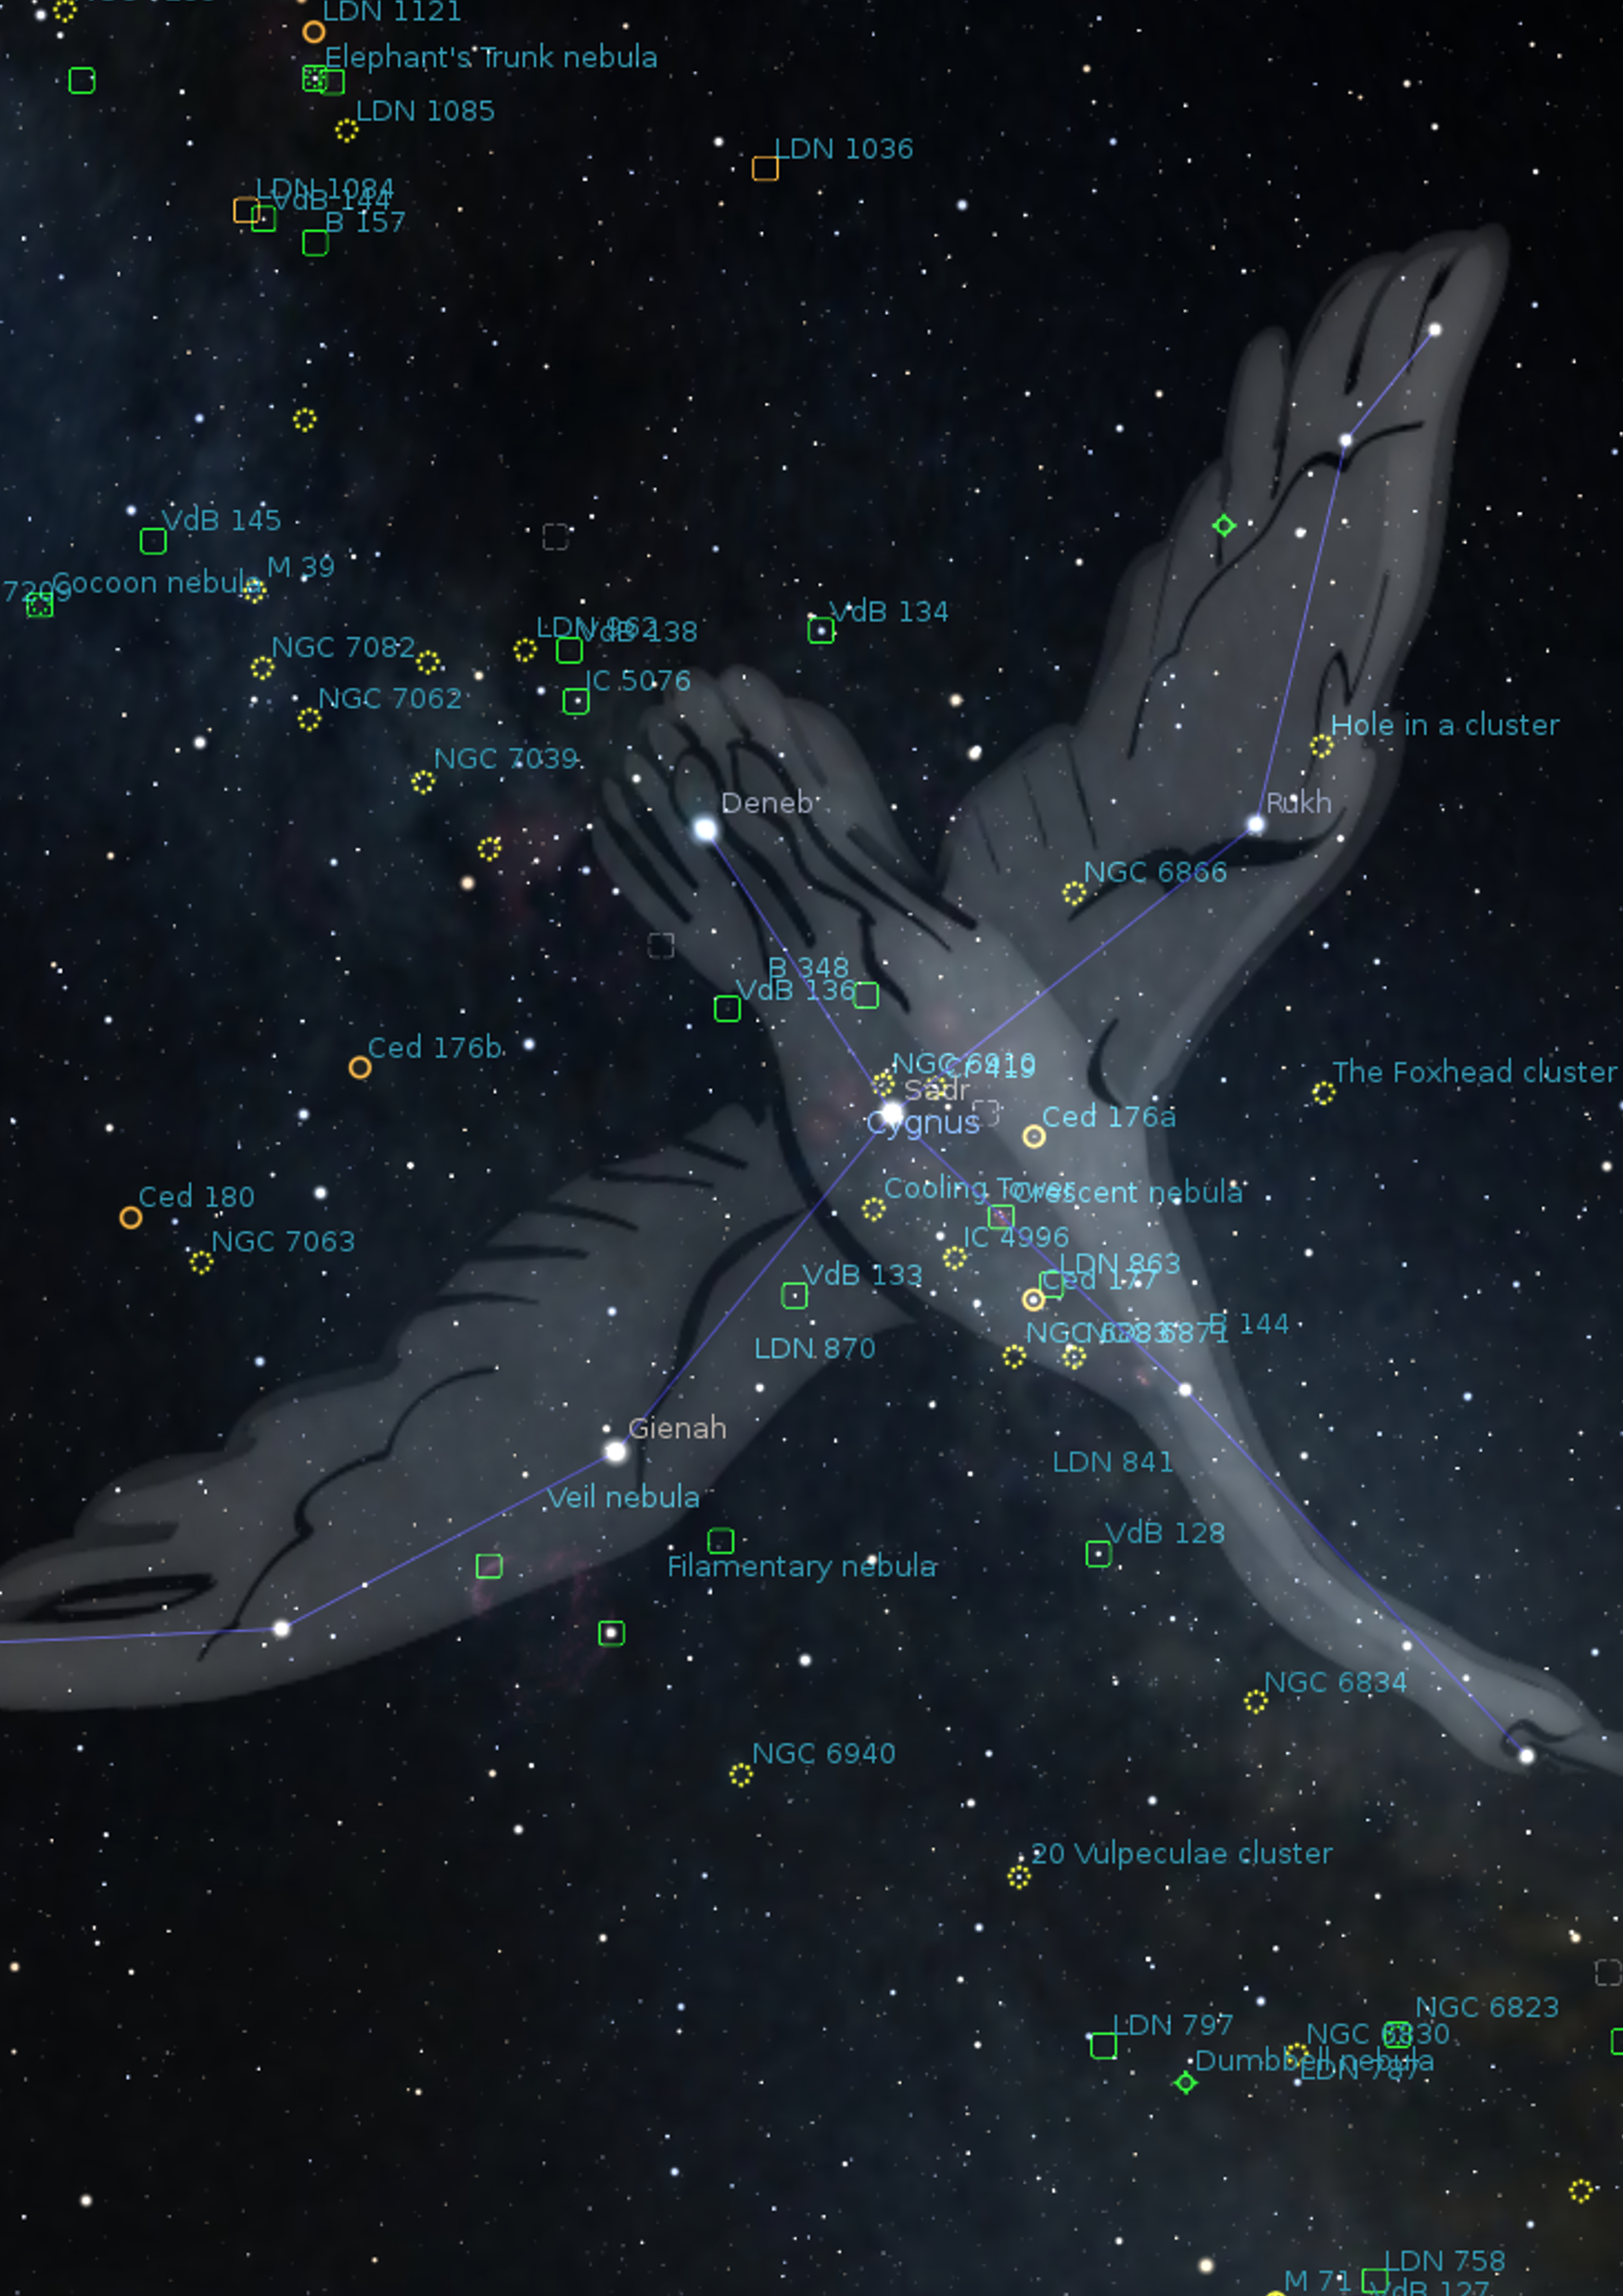
\includegraphics[width=\paperwidth]{bookcover}}; % Background image
\draw[anchor=north] (midpoint) node [fill=ocre!30!white,fill opacity=0.6,text opacity=1,inner sep=1cm]%
     {\Huge\centering\bfseries\sffamily\parbox[c][][t]{\paperwidth}%
                                              {\centering Stellarium User Guide\\[18pt] % Book title
                                              {\Large Matthew Gates, Georg Zotti, Alexander Wolf, Barry Gerdes}\\[15pt]% Author names
                                              {\Large Version \StelVersion-\DocumentEdition}\\[15pt]% Version like 0.15.0-1
                                              {\Large 2016}% Year
                                             }}; % 
\end{tikzpicture}};
\end{tikzpicture}
\vfill
\endgroup

%----------------------------------------------------------------------------------------
%	COPYRIGHT PAGE
%----------------------------------------------------------------------------------------

\newpage
~\vfill
\thispagestyle{empty}

\noindent Copyright \copyright\ 2006-2009 Matthew Gates.\\ % Copyright notice
\noindent Copyright \copyright\ 2014-2016 Georg Zotti.\\ % Copyright notice
\noindent Copyright \copyright\ 2011-2016 Alexander Wolf.\\ % Copyright notice
\noindent Copyright \copyright\ 2013-2014 Barry Gerdes.\\ % Copyright notice

\noindent \fbox{
  \begin{minipage}[t]{0.8\linewidth}
    Stellarium Version 0.15 is dedicated in memory of our team
    member Barry Gerdes (\dag\,2014).
  \end{minipage}
}\\

\noindent \textsc{stellarium.org}\\ % URL

\noindent Permission is granted to copy, distribute and/or modify this
document under the terms of the GNU Free Documentation License,
Version 1.2 or any later version published by the Free Software
Foundation; with no Invariant Sections, no Front-Cover Texts, and no
Back-Cover Texts. A copy of the license is included in
appendix~\ref{ch:License} entitled ``GNU Free Documentation
License''.\\ % License information

\small{\noindent \textit{All trademarks, third party brands, product names, trade names,
corporate names and company names mentioned may be trademarks of their
respective owners or registered trademarks of other companies and are
used for purposes of explanation and to the readers' benefit, without
implying a violation of copyright law.}}\\


\noindent \textit{A version \StelVersion-\DocumentEdition, \today} % Printing/edition date

%----------------------------------------------------------------------------------------
%	TABLE OF CONTENTS
%----------------------------------------------------------------------------------------

\chapterimage{chapter-t1-bg} % Table of contents heading image

\pagestyle{empty} % No headers

\tableofcontents % Print the table of contents itself

\cleardoublepage % Forces the first chapter to start on an odd page so it's on the right

\pagestyle{fancy} % Print headers again


%% There should be one source file per chapter. 
%% Structural changes (chapter images etc.) should be in this main file to better have an overview.
%----------------------------------------------------------------------------------------
%	PART I
%----------------------------------------------------------------------------------------

\part{Basic Use}

%----------------------------------------------------------------------------------------
%	CHAPTER 1 (Introduction)
%----------------------------------------------------------------------------------------
\chapterimage{chapter-t2-bg} % Chapter heading image

% Status info:
% M. Gates	2006-2009
% A. Wolf	2011-2015
% ArdWar	2012
% B. Gerdes	2013
% Additions inserted from wiki 2015-12-26
% Content OK for 0.14+.
% 2016-07: Historical notes added by Fabien.
% TODO: typo&grammar check


\chapter{Introduction}
\label{ch:Introduction}

\emph{Stellarium} is a software project that allows people to use their
home computer as a virtual planetarium. It calculates the positions of
the Sun and Moon, planets and stars, and draws how the sky would look to
an observer depending on their location and the time. It can also draw
the constellations and simulate astronomical phenomena such as meteor
showers or comets, and solar or lunar eclipses.

Stellarium may be used as an educational tool for teaching about the
night sky, as an observational aid for amateur astronomers wishing to
plan a night's observing or even drive their telescopes to observing
targets, or simply as a curiosity (it's fun!). Because of the high
quality of the graphics that Stellarium produces, it is used in some
real planetarium projector products and museum projection setups. Some
amateur astronomy groups use it to create sky maps for describing
regions of the sky in articles for newsletters and magazines, and the
exchangeable sky cultures feature invites its use in the field of
Cultural Astronomy research and outreach.

Stellarium is still under development, and by the time you read
this guide, a newer version may have been released with even more
features than those documented here. Check for updates to Stellarium at
the Stellarium website\footnote{\url{http://stellarium.org}}.

If you have questions and/or comments about this guide, or about
Stellarium itself, visit the Stellarium site at
LaunchPad\footnote{\url{https://launchpad.net/stellarium}} or our
SourceForge
forums\footnote{\url{https://sourceforge.net/p/stellarium/discussion/278769/}}.


\section{Historical notes}
\label{sec:Introduction:HistoricalNotes}

Fabien Ch\'ereau started the project during the summer 2000, and throughout
the years found continuous support by a small team of enthusiastic developers.

Here is a list of past and present major contributors sorted roughly by date of
arrival on the project:
\newpage
\begin{description}
\item[Fabien Ch\'ereau] original creator, maintainer, general development
\item[Matthew Gates] maintainer, original user guide, user support, general development
\item[Johannes Gajdosik] astronomical computations, large star catalogs support
\item[Johan Meuris] GUI design, website creation, drawings of our 88 Western constellations
\item[Nigel Kerr] Mac OSX port
\item[Rob Spearman] funding for planetarium support
\item[Barry Gerdes] user support, tester, Windows support. Barry
  passed away in October 2014 at age 80. He was a major contributor on
  the forums, wiki pages and mailing list where his good will and
  enthusiasm is strongly missed. \ifthenelse{\equal{\StelVersion}{0.15.0}}{Version 0.15 of Stellarium is
  dedicated in his memory.}{} RIP Barry.
\item[Timothy Reaves] ocular plugin
\item[Bogdan Marinov] GUI, telescope control, other plugins
\item[Diego Marcos] SVMT plugin
\item[Guillaume Ch\'ereau] display, optimization, Qt upgrades
\item[Alexander Wolf] maintainer, DSO catalogs, user guide, general development
\item[Georg Zotti] astronomical computations, Scenery 3D and ArchaeoLines plugins, general development, user guide, user support
\item[Marcos Cardinot] MeteorShowers plugin
\item[Florian Schaukowitsch] Scenery 3D plugin, Remote Control plugin, Qt/OpenGL internals
\end{description}

Unfortunately time is evolving, and most members of the original
development team are no longer able to devote most of their spare time
to the project (some are still available for limited work
which requires specific knowledge about the project).

As of 2017, the project's maintainer is Alexander Wolf, doing most maintenance
and regular releases. Major new features are contributed mostly by Georg Zotti
and his team focussing on extensions of Stellarium's applicability in the fields of
historical and cultural astronomy research (which means Stellarium is getting more
accurate), but also on graphic items like comet tails or the Zodiacal Light.

\vspace{1\baselineskip}
\noindent A detailed track of development can be found in the
\file{ChangeLog} file in the installation folder. A few important
milestones for the project:
\begin{description}
\item[2000] first lines of code for the project
\item[2001-06] first public mention (and users feedbacks!) of the
  software on the French newsgroup \texttt{fr.sci.astronomie.amateur} 
  \footnote{\url{https://groups.google.com/d/topic/fr.sci.astronomie.amateur/OT7K8yogRlI/discussion}}
\item[2003-01] Stellarium reviewed by Astronomy magazine
\item[2003-07] funding for developing planetarium features (fisheye projection and other features)
\item[2005-12] use accurate (and fast) planetary model
\item[2006-05] Stellarium ``Project Of the Month'' on SourceForge
\item[2006-08] large stars catalogs
\item[2007-01] funding by ESO for development of professional astronomy extensions (VirGO)
\item[2007-04] developers' meeting near Munich, Germany
\item[2007-05] switch to the Qt library as main GUI and general purpose library
\item[2009-09] plugin system, enabling a lot of new development
\item[2010-07] Stellarium ported on Maemo mobile device
\item[2010-11] artificial satellites plugin
\item[2014-06] high quality satellites and Saturn rings shadows, normal mapping for moon craters
\item[2014-07] V0.13: adapt to OpenGL evolutions in the Qt framework, now requires more modern graphic hardware than earlier versions
\item[2015-04] V0.13.3: Scenery 3D plugin
\item[2015-10] V0.14.0: Accurate precession
\item[2016-07] V0.15: Remote Control plugin
\item[2016-12] V0.15.1: DE430\&DE431, AstroCalc, DSS layer, and Stellarium acting as SpoutSender
\end{description}

Stellarium has been kindly supported by ESA in their Summer of Code in
Space initiatives, which resulted in better planetary rendering
(2012), the Meteor Showers plugin (2013) and the web-based remote
control and an alternative solution for planetary positions based on
the DE430/DE431 ephemeris (2015).


This guide is based on the user guide written by Matthew Gates for
version 0.10 around 2008. The guide was then ported to the Stellarium
wiki and continuously updated by Barry Gerdes and Alexander Wolf up to version 0.12. 

The user documentation has been developed further on the Stellarium
wiki for some time, but without Barry started to fall out of sync with
the actual program.  We (Alexander and Georg) have ported the texts
back to \LaTeX{} and updated and added information where necessary. We
feel now that a single book may be the better format for offline
reading. The PDF version of this guide has a clickable table of
contents and clickable hyperlinks.

This new edition of the guide will not contain notes about using
earlier versions than 0.13 or using very outdated hardware. Some
references to previous version may still be made for completeness, 
but if you are using earlier versions
for particular reasons, please use the older guides.

%%% Local Variables: 
%%% mode: latex
%%% TeX-PDF-mode: t
%%% TeX-master: "guide"
%%% End: 



%----------------------------------------------------------------------------------------
%	CHAPTER 2 (Installation)
%----------------------------------------------------------------------------------------
% \chapterimage{chapter-t2-bg} % Chapter heading image Did not change...

% Status info:
% M. Gates	2006-2009
% A. Wolf	2011-2015
% Lee Carré	2011
% ArdWar	2012
% MisterE	2013
% B. Gerdes	2013
% G. Zotti	2014-2016
% Additions inserted from wiki 2015-12-26
% GZ checked grammar and structure, added ANGLE details and Troubleshooting.
% Content OK for 0.15+.
% TODO: Fix a few TODOs noted below.


\chapter{Getting Started}
\label{ch:GettingStarted}

\section{System Requirements}\index{System Requirements}
\label{sec:GettingStarted:SystemRequirements}

Stellarium has been seen to run on most systems where Qt5 is
available, from tiny ARM computers like the Raspberry Pi~2\footnote{As
  of spring 2016, you need to enable the experimental OpenGL driver
  and compile Stellarium from sources.} or Odroid C1 to big museum
installations with multiple projectors. The most important hardware
requirement is a contemporary graphics subsystem.


\subsection{Minimum}
\begin{itemize}
\item Linux/Unix; Windows 7 and later (It may run on Vista, but unsupported. A special version for XP is still available); OS X 10.8.5 and later
\item 3D graphics card which supports OpenGL 3.0 and GLSL 1.3 (2008
  GeForce 8xxx and later, ATI/AMD Radeon HD-2xxx and later; Intel HD
  graphics (Core-i 2xxx and later)) or OpenGL ES 2.0 and GLSL ES 1.0
  (e.g., ARM SBCs like Raspberry Pi~2). On Windows, some older cards
  may be supported via ANGLE when they support DirectX10.
\item 512 MB RAM
\item 250 MB free on disk
\end{itemize}

\subsection{Recommended}
\begin{itemize}
\item Linux/Unix; Windows 7 and later; OS X 10.8.5 and later
\item 3D graphics card which supports OpenGL 3.3 and above and GLSL1.3 and later
\item 1 GB RAM or more
\item 1.5 GB free on disk (About 3GB extra required for the optional DE430/DE431 files).
\end{itemize}
 A dark room for realistic rendering --- details like the Milky Way, Zodiacal Light or
star twinkling can't be seen in a bright room.


\section{Downloading}\index{Downloading}
\label{sec:GettingStarted:Downloading}

Download the correct package for your operating system directly from the main page, \newline \url{http://stellarium.org}.

\section{Installation}\index{Installation}
\label{sec:GettingStarted:Installation}

\subsection{Windows}\index{Windows}

\begin{enumerate}
\item Double click on the installer file you downloaded:
\begin{itemize}
\item \file{stellarium-\StelVersion-win64.exe} for 64-bit Windows 7 and later.
\item \file{stellarium-\StelVersion-win32.exe} for 32-bit Windows 7 and later.
\item \file{stellarium-\StelVersion-classic-win32.exe} for Windows XP and later.
\end{itemize}
\item Follow the on-screen instructions.
\end{enumerate}

\subsection{OS X}\index{OS X}

\begin{enumerate}
\item
  Locate the \file{Stellarium-\StelVersion.dmg} file in
  Finder and double click on it or open it using the Disk Utility
  application. Now, a new disk appears on your desktop and Stellarium is
  in it.
\item
  Open the new disk and please take a moment to read the \file{ReadMe} file.
  Then drag \file{Stellarium} to the Applications folder.
\item
  Note: You should copy Stellarium to the Applications folder before
  running it --- some users have reported problems running it directly
  from the disk image (\file{.dmg}).
\end{enumerate}

\subsection{Linux}\index{Linux}

Check if your distribution has a package for Stellarium already --- if
so you're probably best off using it. If not, you can download and build
the source.

For Ubuntu we provide a package repository with the latest stable
releases. Open a terminal and type:

\begin{commands}
sudo add-apt-repository ppa:stellarium/stellarium-releases
sudo apt-get update
sudo apt-get install stellarium
\end{commands}


\section{Running Stellarium}\index{Running Stellarium}
\label{sec:GettingStarted:Running}

\subsection{Windows}\index{Windows}
\label{sec:GettingStarted:Running:Windows}

The Stellarium installer creates a whole list of items in the
\textbf{Start Menu} under the \textbf{Programs/Stellarium}
section. The list evolves over time, not all entries listed here 
may be installed on your system. Select one of these to run Stellarium:
\begin{description}
\item[Stellarium] OpenGL version. This is the most efficient for
  modern PCs and should be used when you have installed appropriate
  OpenGL drivers. Note that some graphics cards are ``blacklisted'' by
  Qt to immediately run via ANGLE (Direct3D), you cannot force OpenGL in this
  case. This should not bother you.
\item[Stellarium (ANGLE mode)] Uses Direct3D translation of the OpenGL
  rendering via ANGLE library.  Forces Direct3D version~9.
%  \item[Stellarium (ANGLE WARP mode)] Uses DirectX3D~11 software rendering via ANGLE
%    library. This should work on any PC without dedicated graphics
%    card. However on many systems this fails, it is unclear why.
\item[Stellarium (MESA mode)] Uses software rendering via MESA
  library. This should work on any PC without dedicated graphics card.
  % TODO This note may be obsolete before 0.15 is out when MESA works again.
  % However on some systems this also fails, it is unclear
  % why\footnote{This was the emergency fallback solution for the 0.13
  % series. We have reports that 0.13.2-MESA works on a system where
  % 0.14 does not.}
\end{description}
On startup, a diagnostic check is performed to test whether the
graphics hardware is capable of running. If all is fine, you will see
nothing of it.  Else you may see an error panel informing you that
your computer is not capable of running Stellarium (``No OpenGL~2
found''), or a warning that there is only OpenGL~2.1 support. The
latter means you will be able to see some graphics, but depending on
the type of issue you will have some bad graphics. For example, on an
Intel GMA4500 there is only a minor issue in Night Mode, while on
other systems we had reports of missing planets or even crashes as
soon as a planet comes into view. If you see this, try running in
Direct3D~9 or MESA mode, or upgrade your system. The warning, once
ignored, will not show again.

When you have found a mode that works on your system, you can delete
the other links.

\subsection{OS X}\index{OS X}
\label{sec:GettingStarted:Running:MacOSX}

Double click on the \emph{Stellarium} application.  Add it to your
\textbf{Dock} for quick access.

\subsection{Linux}\index{Linux}
\label{sec:GettingStarted:Running:Linux}

If your distribution had a package you'll probably already have an
item in the GNOME or KDE application menus. If not, just open a
terminal and type \texttt{stellarium}.


\section{Troubleshooting}
\label{sec:GettingStarted:Running:Troubleshooting}

Stellarium writes startup and other diagnostic messages into a
logfile. Please see section~\ref{sec:FilesAndDirectories} where this
file is located on your system. This file is \emph{essential} in case when
you feel you need to report a problem with your system which has not
been found before.

If you don't succeed in running Stellarium, please see the online
forum\footnote{\url{https://launchpad.net/stellarium}}.  It includes
FAQ (Frequently Asked Questions, also Frequently Answered
Questions)\index{FAQ} and a general question section which may include
further hints. Please make sure you have read and understood the FAQ
before asking the same questions again.


%%% Local Variables: 
%%% mode: latex
%%% TeX-PDF-mode: t
%%% TeX-master: "guide"
%%% End: 


%----------------------------------------------------------------------------------------
%	CHAPTER 3 (was called Interface Guide, but is just a first tour.)
%----------------------------------------------------------------------------------------

% Status info:
% M. Gates	2006-2009
% A. Wolf	2011-2014
% B. Gerdes	2013
% Additions inserted from wiki 2015-12-26
% Content OK for 0.12.4.
% 2016-04 GZ started restructuring
% TODO: typo&grammar check

%\chapterimage{chapter-t2-bg} % Chapter heading image (now in guide.tex)

\chapter{A First Tour}
\label{ch:tour}


\begin{figure}[tbh]\centering
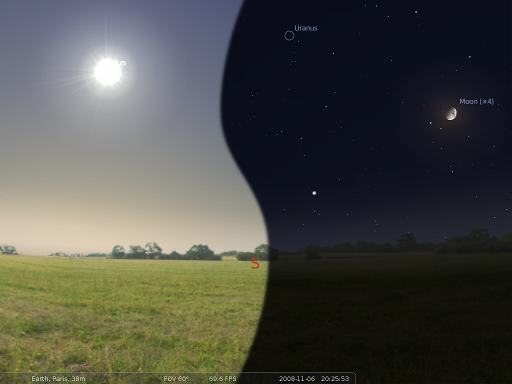
\includegraphics[width=0.95\textwidth,trim=0 0 0 30,clip]{001}
\caption{Stellarium main view. (Combination of day and night views.)}
\label{fig:001}
\end{figure}

\noindent When Stellarium first starts, we see a green meadow under a
sky. Depending on the time of day, it is either a day or night
scene. If you are connected to the Internet, an automatic lookup will
attempt to detect your approximate position.\footnote{See
  section~\ref{sec:gui:location} if you want to switch this off.}

At the bottom left of the screen, you can see the status bar. This shows
the current observer location, field of view (FOV), graphics performance
in frames per second (FPS) and the current simulation date and time.
If you move the mouse over the status bar, it will move up to reveal a
tool bar which gives quick control over the program.

The rest of the view is devoted to rendering a realistic scene including
a panoramic landscape and the sky. If the simulation time and observer
location are such that it is night time, you will see stars, planets and
the moon in the sky, all in the correct positions.

You can drag with the mouse on the sky to look around or use the
cursor keys. You can zoom with the mouse wheel or the \key{Page
  \arrowkeyup} or \key{Page \arrowkeydown} keys.

Much of Stellarium can be controlled very intuitively with the
mouse. Many settings can additionally be switched with shortcut keys
(hotkeys).  Advanced users will learn to use these shortcut
keys. Sometimes a key combination will be used. For example, you can
quit Stellarium by pressing \key{\ctrl+Q} on Windows and Linux, and
\key{\cmdmac+Q} on Mac OS X.  For simplicity, we will show only the
Windows/Linux version. We will present the default hotkeys in this
guide. However, almost all hotkeys can be reconfigured to match your
taste. Note that some listed shortkeys are only available as key
combinations on international keyboard layouts, e.g., keys which
require pressing \key{AltGr} on a German keyboard. These must be
reconfigured, please see~\ref{sec:gui:help:hotkeys} for details.


The way Stellarium is shown on the screen is primarily governed by the
menus. These are accessed by dragging the mouse to the left or bottom
edge of the screen, where the menus will slide out. In case you want
to see the menu bars permanently, you can press the small buttons
right in the lower left corner to keep them visible.


\section{Time Travel}
\label{sec:tour:timeTravel}

When Stellarium starts up, it sets its clock to the same time and date
as the system clock. However, Stellarium's clock is not fixed to the same
time and date as the system clock, or indeed to the same speed. We may
tell Stellarium to change how fast time should pass, and even make time
go backwards! So the first thing we shall do is to travel into the
future! Let's take a look at the time control buttons on the right hand
ride of the tool-bar. If you hover the mouse cursor over the buttons, a
short description of the button's purpose and keyboard shortcut will
appear.

\begin{table}[h]
\centering
\begin{tabular}{c c l}\toprule
\emph{Button} & \emph{Shortcut key} & \emph{Description}\\\midrule
\guibutton[0.75]{2.25}{bt_timerate_decrease} & \key{J} & Decrease the rate at which time passes \\
\guibutton[0.75]{2.25}{bt_timerate_normal}   & \key{K} & Make time pass as normal \\
\guibutton[0.75]{2.25}{bt_timerate_increase} & \key{L} & Increase the rate at which time passes \\
\guibutton[0.75]{2.25}{bt_time_normal}       & \key{8} & Return to the current time \& date \\
\bottomrule
\end{tabular}
\caption{Time Travel}
\end{table}

OK, so lets go see the future! Click the mouse once on the increase time
speed button \guibutton{0.6}{bt_timerate_increase}. 
Not a whole lot seems to happen. However, take a look at the clock in
the status bar. You should see the time going by faster than a normal
clock! Click the button a second time. Now the time is going by faster
than before. If it's night time, you might also notice that the stars
have started to move slightly across the sky. If it's daytime you might
be able to see the sun moving (but it's less apparent than the movement
of the stars). Increase the rate at which time passes again by clicking
on the button a third time. Now time is really flying!

Let time move on at this fast speed for a little while. Notice how the
stars move across the sky. If you wait a little while, you'll see the
Sun rising and setting. It's a bit like a time-lapse movie. 

Stellarium not only allows for moving forward through time -- you can
go backwards too! Click on the real time speed button
\guibutton{0.6}{bt_timerate_normal}.  The stars and/or the
Sun should stop scooting across the sky. Now press the decrease time
speed button \guibutton{0.6}{bt_timerate_decrease} once. Look
at the clock. Time has stopped. Click the decrease time speed button
four or five more times. Now we're falling back through time at quite
a rate (about one day every ten seconds!).

\subsection*{Time Dragging, Time Scrolling}
\label{sec:tour:timeDrag}

Another way to quickly change time is \indexterm{time dragging}. Press
\keys{\ctrl} and slide the mouse along the direction of daily motion to go forward, 
or to the other direction to go backward.

\newFeature{0.15.1}Similarly, pressing \keys{\ctrl} and scrolling the mouse wheel will 
advance time by minutes, pressing \keys{\ctrl+\shift} and 
scrolling the mouse wheel will advance time by hours, \keys{\ctrl+\Alt} by days, 
and finally \keys{\ctrl+\shift+\Alt} by calendar years.


Enough time travel for now. Wait until it's night time, and then click
the real time speed button \guibutton{0.6}{bt_timerate_normal}. With a 
little luck you will now be looking at the night sky.

\section{Moving Around the Sky}
\label{sec:tour:moving}

\begin{table}[h]
\centering
\begin{tabular}{ll}\toprule
\emph{Key}                         & \emph{Description}\\\midrule
Cursor keys \keys{\arrowkeyleft} \keys{\arrowkeyright} \keys{\arrowkeyup} \keys{\arrowkeydown} & Pan the view left, right, up and down \\
\keyPageUp{}/\keyPageDown{}, \keys{\ctrl+\arrowkeyup}/\keys{\ctrl+\arrowkeydown} & Zoom in and out \\
Left mouse button                  & Select an object in the sky \\
Right mouse button                 & Clear selected object \\
Centre mouse button (wheel press)  & Centre selected object and start tracking \\
Mouse wheel                        & Zoom in and out \\ 
\key{\space}                       & Centre view on selected object \\
Forward-slash (\key{/})            & Auto-zoom in to selected object \\
Backslash (\key{\textbackslash{}}) & Auto-zoom out to original field of view \\
\bottomrule
\end{tabular}
\caption{Moving Around the Sky}
\label{tab:tour:moving}
\end{table}

As well as travelling through time, Stellarium lets to look around the
sky freely, and zoom in and out. There are several ways to accomplish
this listed in table~\ref{tab:tour:moving}.

Let's try it. Use the cursors to move around left, right, up and down.
Zoom in a little using the \keyPageUp{} key, and back out again using the
\keyPageDown{}. Press the \key{\textbackslash} key and see how Stellarium returns to the
original field of view (how ``zoomed in'' the view is), and direction of
view.
%% TODO Is this still original behaviour? On German Kbd, this does not work anyways, backslash is a AltGr-combination.

It's also possible to move around using the mouse. If you left-click and
drag somewhere on the sky, you can pull the view around.

Another method of moving is to select some object in the sky (left-click
on the object), and press the \key{Space} key to centre the view on that
object. Similarly, selecting an object and pressing the forward-slash
key \key{/} will centre on the object and zoom right in on it.

The forward-slash \key{/} and backslash \key{\textbackslash} keys auto-zoom in an out to different
zoom levels depending on what is selected. If the object selected is a planet
or moon in a \emph{sub-system} with a lot of moons (e.g.\ Jupiter), the
initial zoom in will go to an intermediate level where the whole
sub-system should be visible. A second zoom will go to the full zoom
level on the selected object. Similarly, if you are fully zoomed in on a
moon of Jupiter, the first auto-zoom out will go to the sub-system zoom
level. Subsequent auto-zoom out will fully zoom out and return the
initial direction of view. For objects that are not part of a
sub-system, the initial auto-zoom in will zoom right in on the selected
object (the exact field of view depending on the size/type of the
selected object), and the initial auto-zoom out will return to the
initial FOV and direction of view.

\section{The Main Tool Bar}
\label{sec:tour:toolbar}

\begin{figure}[htb]
\centering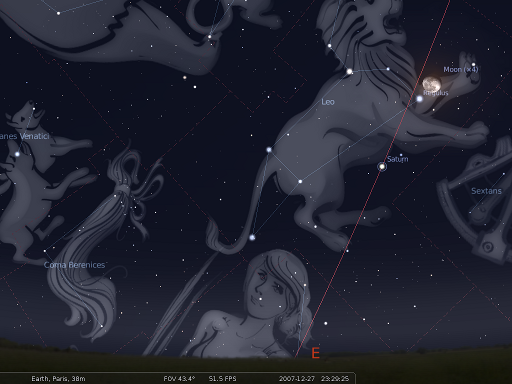
\includegraphics[width=0.9\textwidth]{002}
\caption{Night scene with constellation artwork and moon.}
\label{fig:002}
\end{figure}

Stellarium can do a whole lot more than just draw the stars. Figure~\ref{fig:002}
shows some of Stellarium's visual effects including constellation
line and boundary drawing, constellation art, planet hints, and
atmospheric halo around the bright Moon. The controls in the main tool-bar
provide a mechanism for turning on and off the visual effects.

When the mouse if moved to the bottom left of the screen, a second
tool-bar becomes visible. All the buttons in this side tool-bar open
and close dialog boxes which contain controls for further
configuration of the program. The dialogs will be described in the
next chapter.


Table~\ref{tab:tour:buttons} describes the operations of buttons
on the main tool-bar and the side tool-bar, and gives their default
keyboard shortcuts.

%% TODO: Check default keys!
\newpage
\begin{longtabu} to \textwidth {llcX}\toprule
\emph{Feature}           & \emph{Button} & \emph{Key} & \emph{Description}\\\midrule
Constellations           & \guibutton[0.75]{2.5}{bt_constellation}     & \key{C} & Draw constellations as ``stick figures'' \\
Constellation Names      & \guibutton[0.75]{2.5}{bt_constellation_name}& \key{V} & Draw name of the constellations \\
Constellation Art        & \guibutton[0.75]{2.5}{bt_constellation_art} & \key{R} & Superimpose artistic representations of the constellations \\
Equatorial Grid          & \guibutton[0.75]{2.5}{bt_eq_grid}           & \key{E} & Draw grid lines for the equatorial coordinate system (RA/Dec) \\
Azimuth Grid             & \guibutton[0.75]{2.5}{bt_az_grid}           & \key{Z} & Draw grid lines for the horizontal coordinate system (Alt/Azi) \\
Toggle Ground            & \guibutton[0.75]{2.5}{bt_ground}            & \key{G} & Toggle drawing of the ground. Turn this off to see objects that are below the horizon. \\
Toggle Cardinal Points   & \guibutton[0.75]{2.5}{bt_cardinal}          & \key{Q} & Toggle marking of the North, South, East and West points on the horizon. \\
Toggle Atmosphere        & \guibutton[0.75]{2.5}{bt_atmosphere}        & \key{A} & Toggle atmospheric effects. Most notably makes the stars visible in the daytime.  \\
Deep-Sky Objects         & \guibutton[0.75]{2.5}{bt_nebulae}           & \key{D} & Toggle marking the positions of Deep-Sky Objects. \\
Planet Hints             & \guibutton[0.75]{2.5}{bt_planets}           & \key{P} & Toggle indicators to show the position of planets. \\
Nebula images            & \guibutton[0.75]{2.5}{bt_DSS}        
& \key{I} & Toggle ``nebula images''. This button must be enabled first, see section~\ref{sec:gui:configuration:tools}\\
Digitized Sky Survey     & \guibutton[0.75]{2.5}{bt_ToastSurvey}        
& \key{\ctrl+Alt+D} & Toggle ``Digitized Sky Survey''. This button must be enabled first, see section~\ref{sec:gui:configuration:tools}\\
Coordinate System        & \guibutton[0.75]{2.5}{bt_coord_type}        & \key{\ctrl+M} & Toggle between horizontal (Alt/Azi) \& equatorial (RA/Dec) coordinate systems. \\
Goto                     & \guibutton[0.75]{2.5}{bt_goto}              & \key{\Space} & Center the view on the selected object \\
Night Mode               & \guibutton[0.75]{2.5}{bt_night_mode}        & \key{\ctrl+N} & Toggle ``night mode'', which applies a red-only filter to the view to be easier on the dark-adapted eye. \\
Full Screen Mode         & \guibutton[0.75]{2.5}{bt_fullscreen} & \key{F11} & Toggle full screen mode. \\
Bookmarks                & \guibutton[0.75]{2.5}{bt_bookmarks}        
& \key{Alt+B} & Toggle bookmarks window. This button must be enabled first, see section~\ref{sec:gui:configuration:tools}\\
Flip view (horizontal)   & \guibutton[0.75]{2.5}{bt_fliph}      & \key{\ctrl+Shift+H} & Flip the image in the horizontal plane. This button must be enabled first, see section~\ref{sec:gui:configuration:tools} \\
Flip view (vertical)     & \guibutton[0.75]{2.5}{bt_flipv}      & \key{\ctrl+Shift+V} & Flip the image in the vertical plane. This button must be enabled first, see section~\ref{sec:gui:configuration:tools} \\
Quit Stellarium          & \guibutton[0.75]{2.5}{bt_quit}       & \key{\ctrl+Q} & Close Stellarium.\\
Help Window              & \guibutton[0.5]{2.5}{btd_help}       & \key{F1} & Show the help window, with key bindings and other useful information \\
Configuration Window     & \guibutton[0.5]{2.5}{btd_config}     & \key{F2} & Show the configuration window \\ 
Search Window            & \guibutton[0.5]{2.5}{btd_find}       & \key{F3} or \key{Ctrl+F} & Show the object search window \\
View Window              & \guibutton[0.5]{2.5}{btd_view}       & \key{F4} & Show the view window \\
Time Window              & \guibutton[0.5]{2.5}{btd_time}       & \key{F5} & Show the time window \\
Location Window          & \guibutton[0.5]{2.5}{btd_location}   & \key{F6} & Show the observer location window (map) \\
AstroCalc Window         & \guibutton[0.5]{2.5}{btd_astrocalc}  & \key{F10} & Show the astronomical calculations window \\
\bottomrule
\caption{Stellarium's standard menu buttons}
\label{tab:tour:buttons}
\end{longtabu}


\section{Taking Screenshots}
\label{sec:tour:screenshots}

You can save what is on the screen to a file by pressing
\key{\ctrl+S}. Screenshots are taken in \file{.png} format, and
have filenames like \file{stellarium-000.png},
\file{stellarium-001.png} (the number increments to prevent
overwriting existing files).

Stellarium creates screenshots in a directory depending on
your operating system, see section
\ref{sec:Directories} Files and Directories.







%%% Local Variables: 
%%% mode: latex
%%% TeX-master: "guide"
%%% End: 



%----------------------------------------------------------------------------------------
%	CHAPTER 4 (was called Configuration, but is really an in-depth description of the GUI panels.)
%----------------------------------------------------------------------------------------

% Status info:
% M. Gates	2006-2009
% A. Wolf	2011-2014
% B. Gerdes	2013
% Additions inserted from wiki 2015-12-26
% Content OK for 0.12.4.
% 2016-04 GZ started restructuring
% TODO: typo&grammar check

% \chapterimage{chapter-t2-bg} % Chapter heading image now set in guide.tex

\chapter{The User Interface}
\label{ch:gui}


This chapter describes the dialog windows which can be accessed from the left menu bar.

Most of Stellarium's settings can be changed using the view window
(press \guibutton[0.35]{2}{btd_view} or \key{F4}) and the
configuration window (\guibutton[0.35]{2}{btd_config} or
\key{F2}). Most settings have short labels. To learn more about some
settings, more information is available as \emph{tooltips}, small text
boxes which appear when you hover the mouse cursor over a
button.\footnote{Unfortunately, on Windows~7 and later, with NVidia
  and AMD GPUs, these tooltips often do not work.}

\newFeature{0.15} You can drag the
windows around, and the position will be used again when you restart
Stellarium. If this would mean the window is off-screen (because you
start in windowed mode, or with a different screen), the window will
be moved so that at least a part is visible.

Some options are really rarely changed and therefore may only be
configured by editing the configuration file.  See
\ref{sec:ConfigurationFile} The Main Configuration File for more
details.



\section{Setting the Date and Time}
\label{sec:gui:date}

\begin{figure}[h]
\centering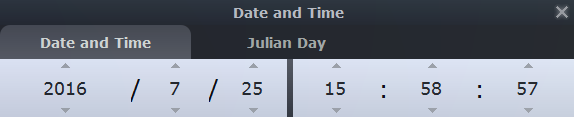
\includegraphics[width=\linewidth]{date_and_time_dialog}
\caption{Date and Time dialog}
\label{fig:gui:date}
\end{figure}

In addition to the time rate control buttons on the main toolbar, you
can use the date and time window (open with the \guibutton[0.35]{2}{btd_time} button or \key{F5}) to set the simulation time. The values
for year, month, day, hour, minutes and seconds may be modified by
typing new values, by clicking the up and down arrows above and below
the values, and by using the mouse wheel.

The other tab in this window allows you to see or set
\indexterm{Julian Day} and/or \indexterm[Julian Day!Modified]{Modified Julian Day} numbers
(see~\ref{sec:Concepts:JulianDay}).

\section{Setting Your Location}
\label{sec:gui:location}

\begin{figure}[htb]
\centering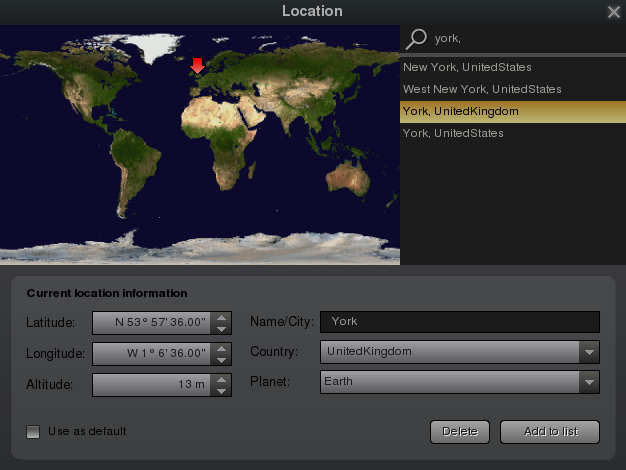
\includegraphics[width=\linewidth]{location_dialog}
\caption{Location window}
\label{fig:gui:location}
\end{figure}

The positions of the stars in the sky is dependent on your location on
Earth (or other planet) as well as the time and date. For Stellarium to
show accurately what is (or will be/was) in the sky, you must tell it
where you are. You only need to do this once -- Stellarium can save your
location so you won't need to set it again until you move.

\newFeature{0.13.1}
After installation, Stellarium uses an online service which tries to
find your approximate location based on the IP address you are
using. This seems very practical, but if you feel this causes privacy
issues, you may want to switch this feature off. You should also consider switching it off on a computer which does not move, to save network bandwidth.

To set your location more accurately, or if the lookup service fails,
press \key{F6} to open the location window (Fig.~\ref{fig:gui:location}). 
There are a few ways you can set your location:

\begin{enumerate}
\item Just click on the map.
\item Search for a city where you live using the search edit box at
  the top right of the window, and select the right city from the
  list.
\item Click on the map to filter the list of cities in the vicinity of
  your click, then choose from the shortlist.
\item Enter a new location using the longitude, latitude and other
  data.
\item Click on \button{Get Location from GPS} if you have a GPS receiver. \newFeature{0.16}
  See section~\ref{sec:ExtraData:GPS} for configuration details. 
  Sometimes you have to try several times to get a valid 3D fix including altitude.
\end{enumerate}

\noindent If you want to use the current location permanently, click on the
``use as default'' checkbox, disable ``Get location from Network'',
and close the location window.



\section{The Configuration Window}
\label{sec:gui:configuration}

The configuration window contains general program settings, and many
other settings which do not concern specific display options. Press
the tool button \guibutton[0.35]{2}{btd_config} or \key{F2} to open.


\subsection{The Main Tab}
\label{sec:gui:configuration:main}


\begin{figure}[bp]
\centering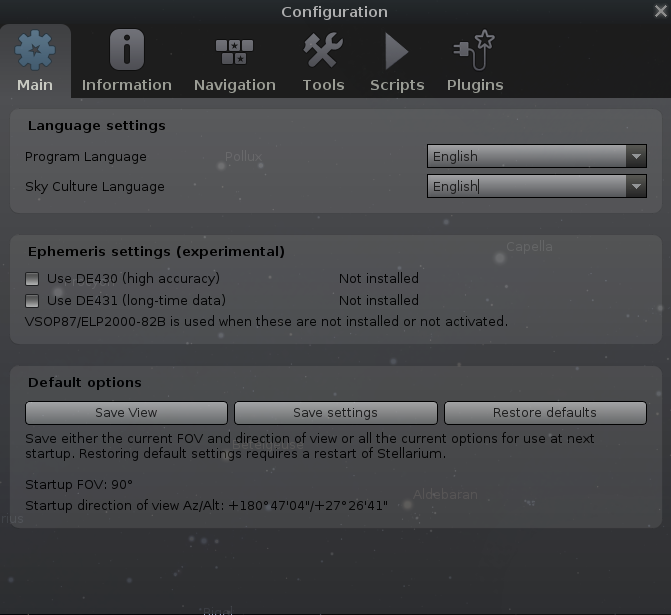
\includegraphics[width=0.65\linewidth]{config_dialog_main_tab}
\caption{Configuration Window: Main Tab}
\label{fig:gui:configuration:main}
\end{figure}

The Main tab in the configuration window provides controls for
changing separately the program and sky culture languages.

The next setting group allows to enable using DE430/DE431 ephemeris
files. Most users do not require this. Thes files have to be installed
separately. See section~\ref{sec:ExtraData:ephemerides} if you are
interested.

The tab also provides a button for saving the current program
configuration. Most display settings have to be explicitly stored to
make a setting change permanent.

\subsection{The Information Tab}
\label{sec:gui:configuration:info}


\begin{figure}[p]
\centering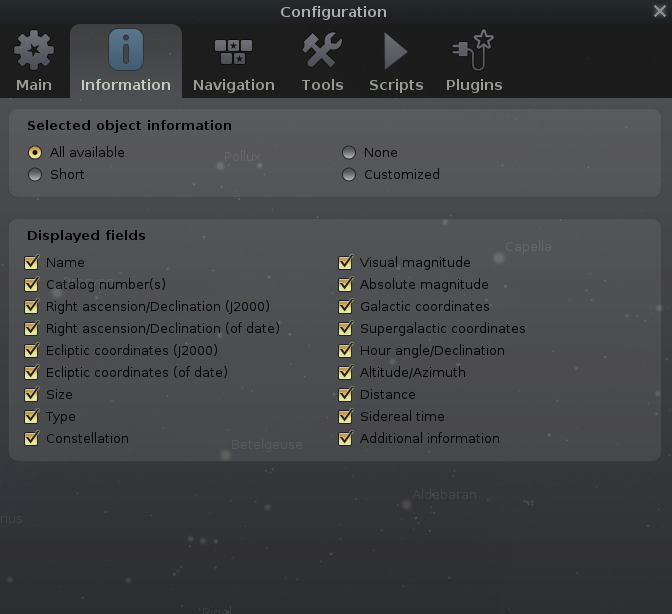
\includegraphics[width=0.65\linewidth]{config_dialog_info_tab}
\caption{Configuration Window: Information Tab}
\label{fig:gui:configuration:info}
\end{figure}

The Information tab allows you to set the type and amount of information
displayed about a selected object.
\begin{itemize}
\item Ticking or unticking the relevant boxes will control this.
\item The information displays in various colours depending on the type and
level of the stored data
\end{itemize}

\subsection{The Navigation Tab}
\label{sec:gui:configuration:nav}


\begin{figure}[p]
\centering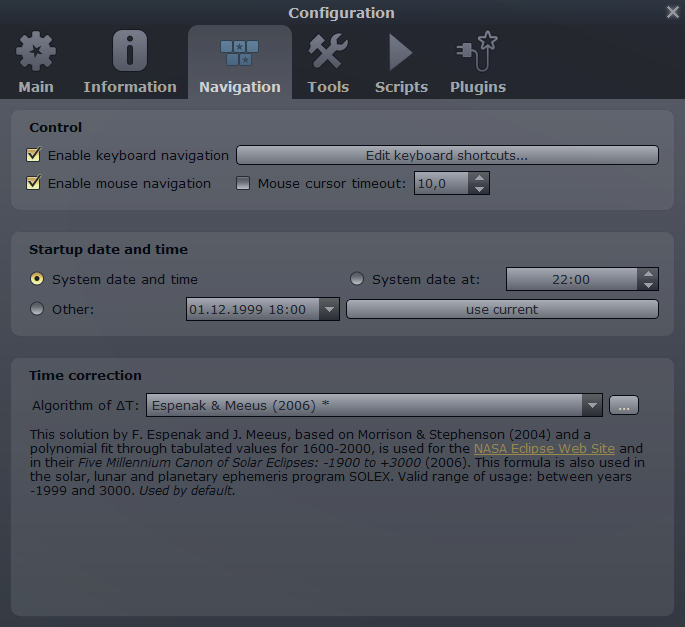
\includegraphics[width=0.65\linewidth]{config_dialog_navigation_tab}
\caption{Configuration Window: Navigation Tab}
\label{fig:gui:configuration:nav}
\end{figure}

The Navigation tab (Fig.~\ref{fig:gui:configuration:nav}) allows for
enabling/disabling of keyboard shortcuts for panning and zooming the
main view, and also how to specify what simulation time should be used
when the program starts:

\begin{description}
\item[System date and time] Stellarium will start with
  the simulation time equal to the operating system clock.
\item[System date at] Stellarium will start with the
  same date as the operating system clock, but the time will be fixed at
  the specified value. This is a useful setting for those people who use
  Stellarium during the day to plan observing sessions for the upcoming
  evening.
\item[Other] some fixed time can be chosen which will
  be used every time Stellarium starts.
\end{description}

The lowest field allows selection of the correction model for the time
correction $\Delta T$ (see section~\ref{sec:Concepts:DeltaT}). Default
is ``Espenak and Meeus (2006)''. Please use other values only if you
know what you are doing.

\subsection{The Tools Tab}
\label{sec:gui:configuration:tools}


\begin{figure}[p]
\centering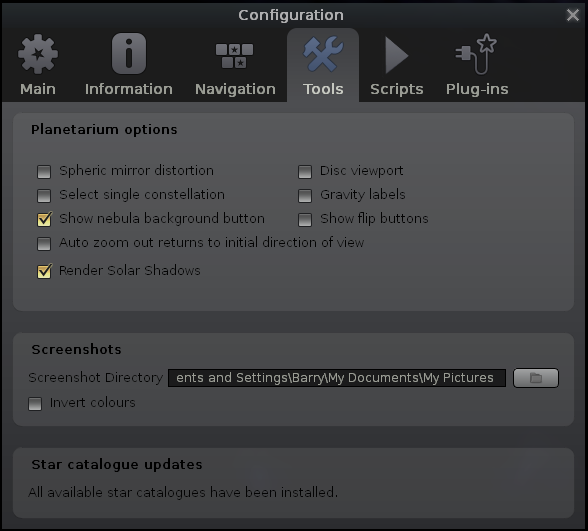
\includegraphics[width=0.65\linewidth]{config_dialog_tools_tab}
\caption{Configuration Window: Tools Tab}
\label{fig:gui:configuration:tools}
\end{figure}

\begin{figure}[p]
\centering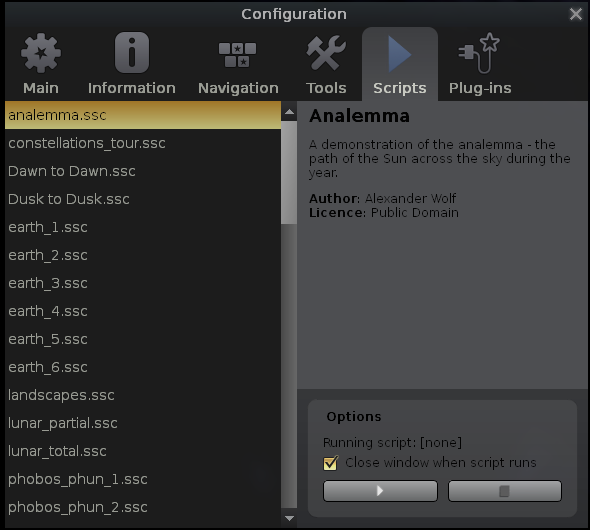
\includegraphics[width=0.65\linewidth]{config_dialog_scripts_tab}
\caption{Configuration Window: Scripts Tab}
\label{fig:gui:configuration:scripts}
\end{figure}

\begin{figure}[p]
\centering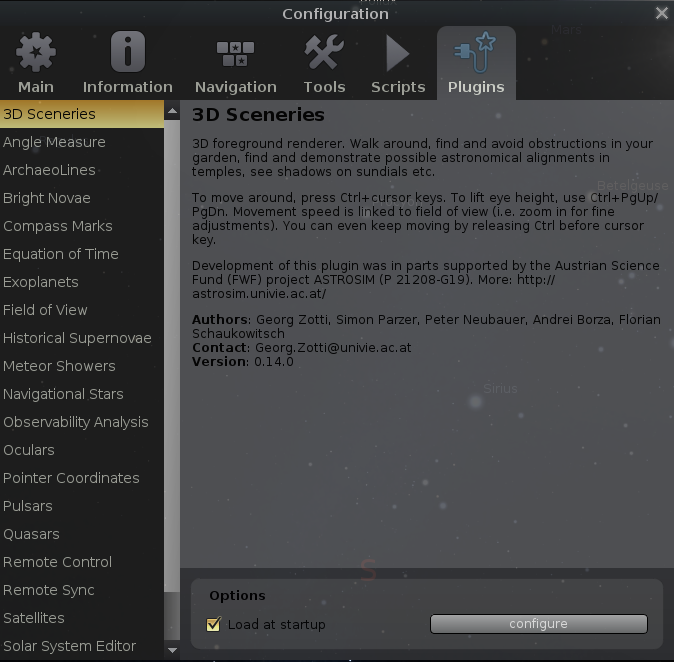
\includegraphics[width=0.65\linewidth]{config_dialog_plugins_tab}
\caption{Configuration Window: Plugins Tab}
\label{fig:gui:plugins}
\end{figure}


The Tools tab (Fig.~\ref{fig:gui:configuration:tools}) contains miscellaneous utility
features:

\begin{description}
\item[Spheric mirror distortion] This option pre-warps the main view
  such that it may be projected onto a spherical mirror using a
  projector. The resulting image will be refected up from the spherical
  mirror in such a way that it may be shone onto a small planetarium
  dome, making a cheap planetarium projection system.
\item[Select single constellation] When active, clicking on a star
  that is member in the constellation lines will make the
  constellation stand out. You can select several constellations, but
  clicking onto a star which is not member of a constellation line
  will display all constellations.
\item[Show nebula background button] You can disable display of DSO
  photographs with this button.
\item[Auto-enabling for the atmosphere] When changing planet during
  location change, atmosphere will be switched as required.
\item[Include nutation] Compute the slight wobble of earth's
  axis. This feature is active only about 500 years around J2000.0.
\item[Azimuth from South] Some users may be used to counting azimuth
  from south.
\item[Disc viewport] This option masks the main view
  producing the effect of a telescope eyepiece. It is also useful when
  projecting Stellarium's output with a fish-eye lens planetarium
  projector.
\item[Gravity labels] This option makes labels of objects in the
  main view align with the nearest horizon. This means that labels
  projected onto a dome are always aligned properly.
\item[Show flip buttons] When enabled, two buttons will be added to
  the main tool bar which allow the main view to be mirrored in the
  vertical and horizontal directions. This is useful when observing
  through telecopes which may cause the image to be mirrored.
\item[Use decimal degrees]
\item[Topocentric coordinates] If you require planetocentric
  coordinates, you may switch this off. Usually it should be enabled.
\item[Auto select landscapes] When changing the planet in the location
  panel, a fitting landscape panorama will be shown when available.
\item[Auto zoom out returns to initial field of view] When enabled,
  this option changes the behaviour of the zoom out key
  (\textbackslash{}) so that it resets the initial direction of view in
  addition to the field of view.
\end{description}

\subsection{The Scripts Tab}
\label{sec:gui:scripts}


The Scripts tab (Fig.~\ref{fig:gui:configuration:scripts}) allows the
selection of pre-assembled scripts bundled with Stellarium that can be
run (See chapter~\ref{ch:scripting} for an introduction to the
scripting capabilities and language). This list can be expanded by
your own scripts as required. See
section~\ref{sec:FilesAndDirectories:DirectoryStructure} where to
store your own scripts.

When a script is selected it can be run by pressing the arrow button
and stopped with the stop button. With some scripts the stop button is
inhibited until the script is finished. %% TODO: EXPLAIN HOW?

Scripts that use sound or embedded videos will need a version of
Stellarium configured at compile time with multimedia support
enabled. It must be pointed out here that sound or video codecs
available depends on the sound and video capabilities of you computer
platform and may not work.


\subsection{The Plugins Tab}
\label{sec:gui:configuration:plugins}


Plugins (see chapter~\ref{ch:Plugins} for an introduction) can be
enabled here (Fig.~\ref{fig:gui:plugins}) to be loaded the next time
you start Stellarium. When loaded, many plugins allow additional configuration
which is available by pressing the \button{configure} button on this tab.




\section{The View Settings Window}
\label{sec:gui:view}

The View settings window controls many display features of Stellarium
which are not available via the main toolbar.

\subsection{The Sky Tab}
\label{sec:gui:view:sky}

\begin{figure}[t]
\centering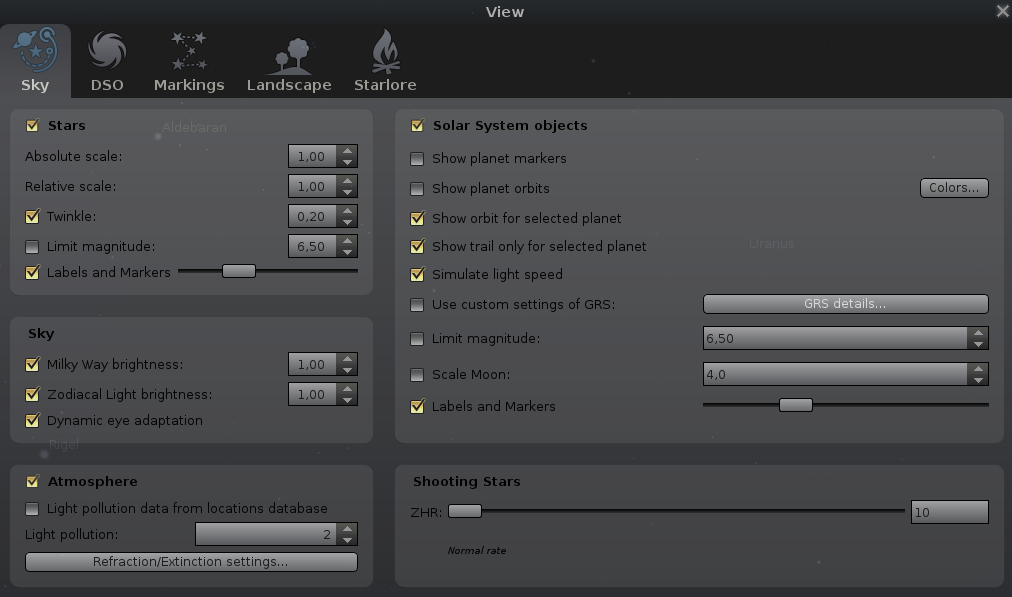
\includegraphics[width=\textwidth]{view_dialog_sky_tab}
\caption{View Settings Window: Sky Tab}
\label{fig:gui:view:sky}
\end{figure}

The Sky tab of the View window (Fig.~\ref{fig:gui:view:sky}) contains settings
for changing the general appearance of the main sky view. Some
hightlights:

\begin{description}
\item[Absolute scale] is the size of stars as rendered by
  Stellarium. If you increase this value, all stars will appear larger
  than before.
\item[Relative scale] determines the difference in size of bright
  stars compared to faint stars. Values higher than 1.00 will make the
  brightest stars appear much larger than they do in the sky. This is
  useful for creating star charts, or when learning the basic
  constellations.
\item[Twinkle] controls how much the stars twinkle when atmosphere is
  enabled (\indexterm{scintillation}, see section~\ref{sec:phenomena:Scintillation}). 
  Since V0.15, the twinkling is reduced in higher altitudes,
  where the star light passes the atmosphere in a steeper angle and is
  less distorted.
\item[Limit magnitude] Inhibits automatic addition of fainter stars
  when zooming in. This may be helpful if you are interested in naked
  eye stars only.
\item[Dynamic eye adaptation] When enabled this feature reduces the
  brightness of faint objects when a bright object is in the field of
  view. This simulates how the eye can be dazzled by a bright object
  such as the moon, making it harder to see faint stars and galaxies.
\item[Light pollution] In urban and suburban areas, the sky is
  brightned by terrestrial light pollution reflected in the atmophere.
  Stellarium simulates light pollution and is calibrated to the
  \emph{Bortle Dark Sky Scale} where 1 means a good dark sky, and 9 is
  a very badly light-polluted sky. See Appendix~\ref{ch:BortleScale}
  for more information.
\item[Solar System objects] this group of options lets you turn on
  and off various features related to the planets. Simulation of light
  speed will give more precise positions for planetary bodies which move
  rapidly against backround stars (e.g. the moons of Jupiter). The
  \emph{Scale Moon} option will increase the apparent size of the moon
  in the sky, which can be nice for wide field of view shots.
\item[Labels and markers] you can independantly change the amount of
  labels displayed for planets, stars and nebuulae. The further to the
  right the sliders are set, the more labels you will see. Note that
  more labels will also appear as you zoom in.
\item[Shooting stars] Stellarium has a simple meteor simulation
  option. This setting controls how many shooting stars will be shown.
  Note that shooting stars are only visible when the time rate is 1, and
  might not be visiable at some times of day. Meteor showers are not
  currently simulated.
\end{description}

\subsubsection{Atmosphere settings}
\label{sec:gui:view:sky:atmosphere}

An auxiliary dialog contains detail settings for the atmosphere. Here
you can set atmospheric pressure and temperature which influence
refraction (see section~\ref{sec:phenomena:Refraction}), and the
opacity factor for extinction, \emph{magnitude loss per airmass} $k$
(see section~\ref{sec:phenomena:Extinction}).


\subsection{The Deep-Sky Objects (DSO) Tab}
\label{sec:gui:view:dso}

\begin{figure}[t]
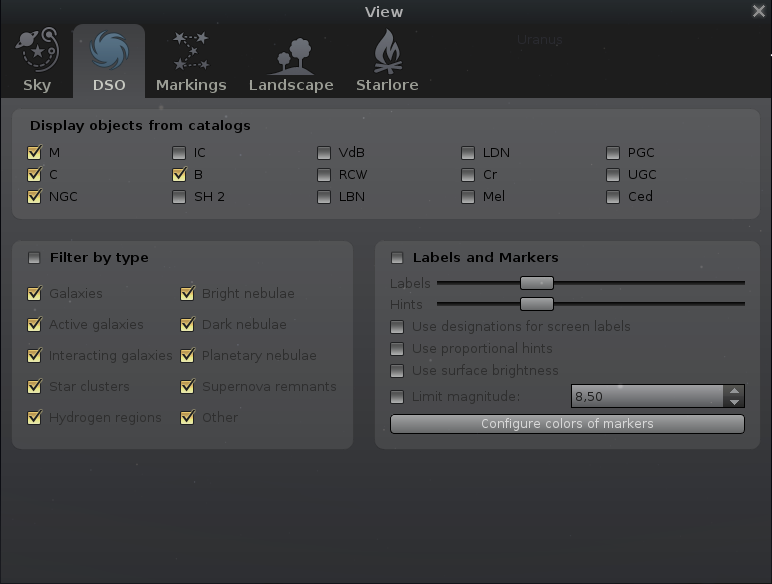
\includegraphics[width=\textwidth,trim=0 70 0 0,clip]{view_dialog_dso_tab}
\caption{View Settings Window: DSO Tab}
\label{fig:gui:view:dso}
\end{figure}


\indexterm{Deep-sky objects} or DSO are extended objects which are
external to the solar system, and are not point-sources like stars.
DSO include galaxies, planetary nebulae and star clusters. These
objects may or may not have images associated with them. Stellarium
comes with a catalogue with over 83,000 extended objects containing
the combined data from many catalogues, with 200 images.  The DSO tab
(Fig.~\ref{fig:gui:view:dso}) allows you to specify which catalogs or
which object types you are interested in. See chapter~\ref{ch:DSO} for
details about the catalog, and how to extend it with your own photographs.





\subsection{The Markings Tab}
\label{sec:gui:view:markings}

\begin{figure}[t]
\centering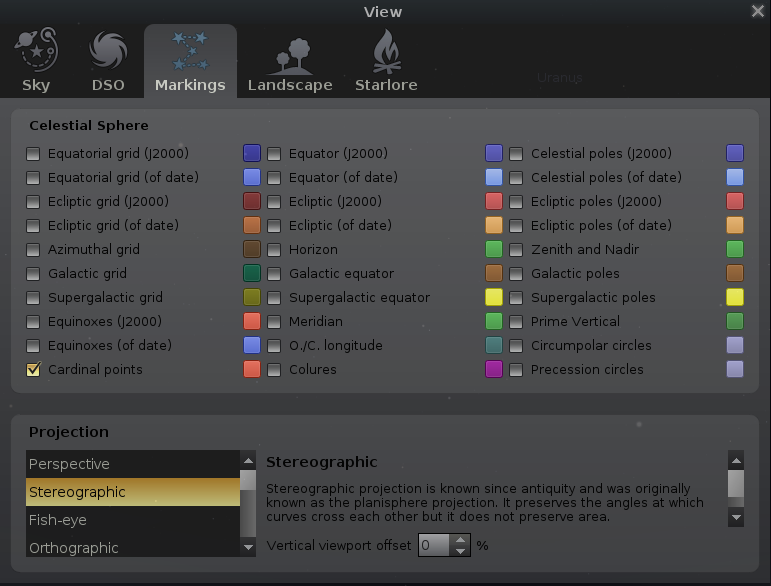
\includegraphics[width=\textwidth]{view_dialog_markings_tab}
\caption{View Settings Window: Markings Tab}
\label{fig:gui:view:markings}
\end{figure}

The Markings tab of the View window
(Fig.~\ref{fig:gui:view:markings}) controls the following features:

\begin{description}
\item[Celestial sphere] this group of options makes it possible to
  plot various grids and lines in the main view.
\item[Projection] Selecting items in this list changes the
  projection method which Stellarium uses to draw the sky~\cite{Snyder:MapProjections}. Options are:

  \begin{description}
  \item[Perspective] Perspective projection maps the horizon and other
    great circles like equator, ecliptic, hour lines, etc. into
    straight lines. The maximum field of view is 150\degree. The
    mathematical name for this projection method is \emph{gnomonic
      projection}.
  \item[Stereographic] Stereographic projection has been known since
    antiquity and was originally known as the planisphere
    projection. It preserves the angles at which curves cross each
    other but it does not preserve area. Else it is similar to
    fish-eye projection mode. The maximum field of view in this mode
    is 235\degree.
  \item[Fish-Eye] Stellarium draws the sky using \emph{azimuthal
    equidistant projection}. In fish-eye projection, straight lines
    become curves when they appear a large angular distance from the
    centre of the field of view (like the distortions seen with very
    wide angle camera lenses). This is more pronounced as the user zooms
    out. The maximum field of view in this mode is 180\degree.
  \item[Orthographic] Orthographic projection is related to
    perspective projection, but the \emph{point of perspective} is set
    to an infinite distance. The maximum field of view is 180\degree.
  \item[Equal Area] The full name of this projection method is
    \emph{Lambert azimuthal equal-area projection}. It preserves the
    area but not the angle. The maximum field of view is 360\degree.
  \item[Hammer-Aitoff] The Hammer projection is an equal-area map
    projection, described by \name[Ernst von]{Hammer} (1858--1925) in 1892 and directly inspired
    by the Aitoff projection. The maximum field of view in this mode is
    360\degree.
  \item[Sinusoidal] The sinusoidal projection is a
    \emph{pseudocylindrical equal-area map projection}, sometimes
    called the Sanson--Flamsteed or the Mercator equal-area
    projection. Meridians are mapped to sine curves.
  \item[Mercator] Mercator projection is a cylindrical projection developed 
    by \name[Gerardus]{Mercator} (1512--1594)
    which preserves the angles between objects, and the scale around
    an object is the same in all directions. The poles are mapped to
    infinity.  The maximum field of view in this mode is 233\degree.
  \item[Miller cylindrical] The Miller cylindrical projection is a
    modified Mercator projection, proposed by \name[Osborn Maitland]{Miller}
    (1897--1979) in 1942. The poles are no longer mapped to
    infinity.
  \item[Cylinder] The full name of this simple projection mode is
    \emph{cylindrical equidistant projection} or \emph{Plate
      Carr\'ee}. The maximum field of view in this mode is 233\degree.
  \end{description}
\end{description}

\subsection{The Landscape Tab}
\label{sec:gui:view:landscape}

\begin{figure}[t]
\centering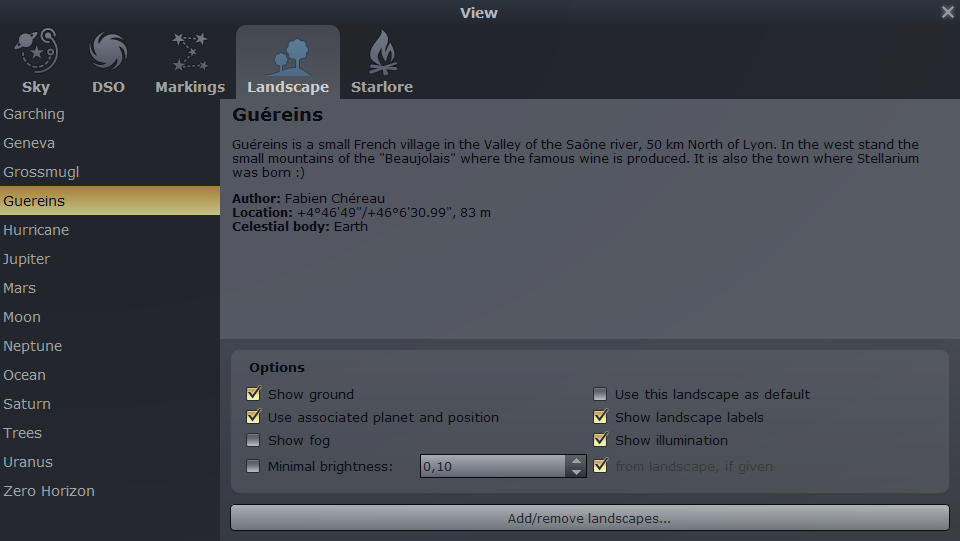
\includegraphics[width=\textwidth]{view_dialog_landscape_tab}
\caption{View Settings Window: Landscape Tab}
\label{fig:gui:view:landscape}
\end{figure}

The Landscape tab of the View window
(Fig.~\ref{fig:gui:view:landscape}) controls the landscape graphics
(the horizon which surrounds you). To change the landscape graphics,
select a landscape from the list on the left side of the window. A
description of the landscape will be shown on the right.

Note that while a landscape  can include information about where the
landscape graphics were taken (planet, longitude, latitude and
altitude), this location does not have to be the same as the location
selected in the Location window, although you can set up Stellarium such
that selection of a new landscape will alter the location for you.

The controls at the bottom right of the window operate as follows:

\begin{description}
\item[Show ground] This turns on and off landscape rendering (same
  as the button \guibutton{0.6}{bt_ground} in the main tool-bar).
\item[Show\_fog] This turns on and off rendering of a band of
  fog/haze along the horizon, when available in this landscape.
\item[Use associated planet and position] When enabled, selecting a
  new landscape will automatically update the observer location.
\item[Use this landscape as default] Selecting this option will save
  the landscape into the program configuration file so that the current
  landscape will be the one used when Stellarium starts.
\item[Minimal brightness] Use some minimal brightness
  setting. Moonless night on very dark locations may appear too dark
  on your screen. You may want to configure some minimal brightness
  here.
\item[from landscape, if given] Landscape authors may decide to
  provide such a minimal brightness value in the \file{landscape.ini}
  file.
\item[Show landscape labels] Landscapes can be configured with a
  gazetteer of interesting points, e.g., mountain peaks, which can be
  labeled with this option.
\item[Show illumination] to reflect the ugly developments of our
  civilisation, landscapes can be configured with a layer of light
  pollution, e.g., streetlamps, bright windows, or the sky glow of a
  nearby city. This layer, if present, will be mixed in when it is
  dark enough.
\end{description}

\noindent Using the button \menu{Add/remove landscapes\ldots}, you can also
install new landscapes from ZIP files which you can download e.g.\
from the Stellarium
website\footnote{\url{http://stellarium.org/wiki/index.php/Landscapes}}
or create yourself (see ch.~\ref{ch:landscapes} Landscapes), or remove
these custom landscapes.

Loading large landscapes may take several seconds. 
If you like to switch rapidly between several landscapes and have enough memory, 
you can increase the default cache size to keep more landscapes loaded previously 
available in memory. Note that a large landscape can take up 200MB or more! 
See section \ref{sec:config.ini:landscape}.

\subsection{The Starlore Tab}
\label{sec:gui:view:starlore}

\begin{figure}[t]
\centering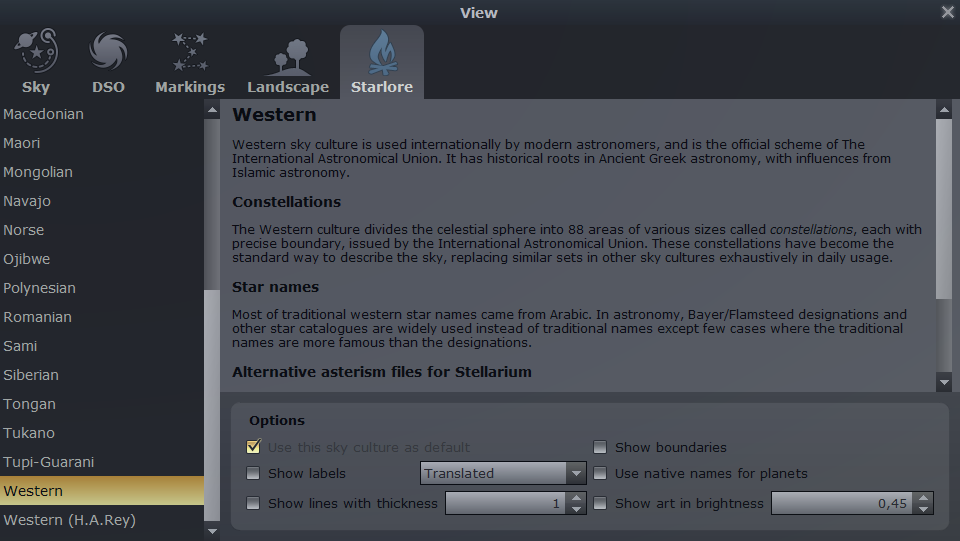
\includegraphics[width=\textwidth]{view_dialog_starlore_tab}
\caption{View Settings Window: Starlore Tab}
\label{fig:gui:view:starlore}
\end{figure}

The Starlore tab of the View window (Fig.~\ref{fig:gui:view:starlore})
controls what culture's constellations and bright star names will be
used in the main display.  Some cultures have constellation art (e.g.,
Western and Inuit), and the rest do not. Configurable options include
\begin{description}
\item[Use this skyculture as default] Activate this option to load
  this skyculture when Stellarium starts.
\item[Show labels] Activate display of constellation labels, like
  \guibutton{0.6}{bt_constellation_name} or \keys{V}. You can further
  select whether you want to display abbreviated, original or
  translated names.
\item[Show lines with thickness\ldots] Activate display of stick
  figures, like \guibutton{0.6}{bt_constellation} or \keys{C}, and you
  can configure constellation line thickness here.
  \item[Show asterism lines\ldots] Activate display of stick figures of asterisms 
  (like the shortcut \keys{Alt+A}) and you can configure asterism line thickness here.
\item[Show boundaries] Activate display of constellation boundaries,
  like \keys{B}. Currently, boundaries have been defined only for
  ``Western'' skycultures.
\item[Use native names for planets] If provided, show the planet names
  as used in this skyculture (also shows modern planet name for
  reference). %% TODO THIS FEATURE NEEDS SOME REWORK!
\item[Show art in brightness\ldots] Activate display of constellation
  art (if available), like \guibutton{0.6}{bt_constellation_art} or
  \keys{R}. You can also select the brightness here.
\item[Show asterism labels] Activate display of asterism labels, like \keys{Alt+V}.
\end{description}


\section{The Object Search Window}
\label{sec:gui:search}

\begin{figure}[p]
\centering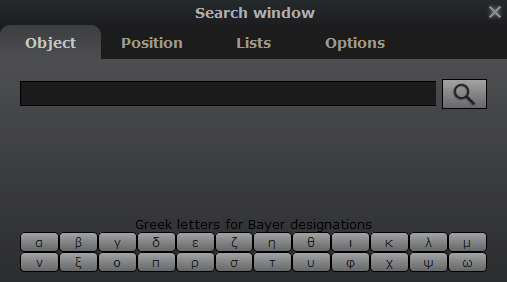
\includegraphics[width=0.68\linewidth]{search_dialog}
\caption{The Search Window: Objects}
\label{fig:gui:search}
\end{figure}

\begin{figure}[p]
\centering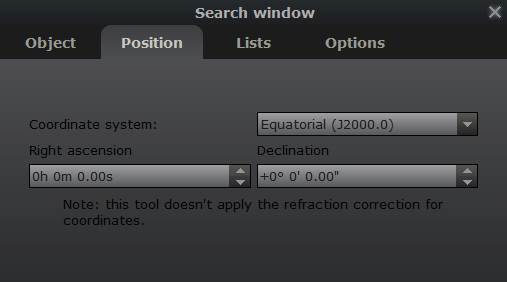
\includegraphics[width=0.68\linewidth]{search_dialog_position}
\caption{The Search Window: Positions}
\label{fig:gui:search:position}
\end{figure}

\begin{figure}[p]
\centering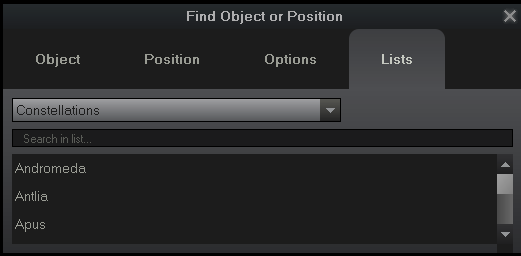
\includegraphics[width=0.68\linewidth]{search_dialog_list}
\caption{The Search Window: Lists}
\label{fig:gui:search:lists}
\end{figure}


\begin{figure}[tp]
\centering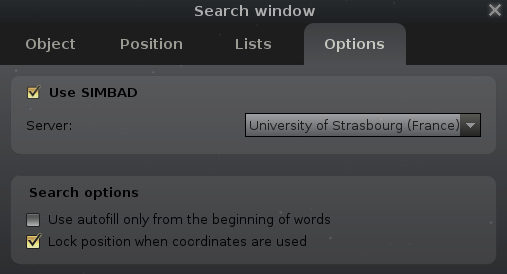
\includegraphics[width=0.68\linewidth]{search_dialog_option}
\caption{The Search Window: Options}
\label{fig:gui:search:options}
\end{figure}

The Object Search window provides a convenient way to locate objects
in the sky. Simply type in the name of an object to find, and press
\key{\return}. Stellarium will point you at that object in the sky.

As you type, Stellarium will make a list of objects which contains 
what you have typed so far. The first of the list of matching objects
will be highlighted. If you press the \key{\tab} key, the selection will change
to the next item in the list. Hitting the \key{\return} key will go to the
currently highlighted object and close the search dialog.

For example, suppose we want to locate Mimas (a moon of Saturn). After
typing the first letter of the name, \emph{m}, Stellarium makes a list
of objects whose name contains M: Haumea, Miranda, Umbriel, \ldots 

You may want at this point to have Stellarium rather propose object
names with start with the string you enter. Do that in the Options tab
of this panel. Now repeat searching (delete, and re-enter M to start
over). Now the list is shorter and contains only objects which start
with M: Maia, Mars, \ldots The first item in this list, Maia, is
highlighted. Pressing \key{\return} now would go to Maia, but we want
Mimas. We can either press \key{\tab} a few times to highlight Mimas
and then hit \key{\return}, or we can continue to type the name until
it is the first/only object in the list.


The Position tab provides a convenient way to enter a set
of coordinates.


The List Search tab allows selection of an object from predefined
sets.  The number of choices is governed by the loaded plug
ins. Simply scroll down the first window to select the type. The name
of an object can then be selected from the list. Press \key{\return} and
Stellarium will go to that object.


The Options tab provides a few settings to fine-tune your search experience.
When the name of an object to find is typed in the object
window and you are connected to the internet and ``Extend search'' is
ticked, Stellarium will search the SIMBAD on-line  data bases for its
coordinates. You can then click the \guibutton{0.6}{bt_search} button or press return.
Stellarium will point you at that object in the sky even if there is no
object displayed on the screen. The SIMBAD server being used can be
selected from the scroll window.


\section{The Astronomical Calculations Window}
\label{sec:gui:AstroCalc}

\newFeature{V0.15.0} This window provides advanced functionality and is still in an experimental phase. You can call it by pressing \key{F10} or button \guibutton{0.6}{btd_astrocalc} on the left bar. The Astronomical Calculations window shows four tabs with different functionality.

\subsection{The Planet Positions Tab}
\label{sec:gui:AstroCalc:Positions}

Shows J2000.0 positions and magnitudes for all installed planets, planet moons, minor bodies (asteroids, comets, etc.) with horizon and magnitude filters. Clicking on an entry brings the object into focus (Figure~\ref{fig:gui:AstroCalc:Positions}).


\begin{figure}[htbp]
\centering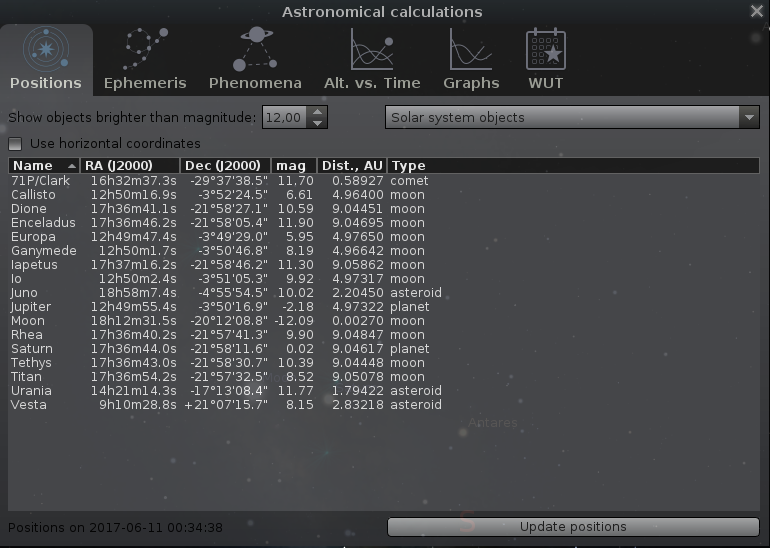
\includegraphics[width=0.68\textwidth]{astrocalc_dialog_positions_tab}
\caption{Astronomical Calculations (AstroCalc): Planetary positions.}
\label{fig:gui:AstroCalc:Positions}
\end{figure}

\subsection{The Celestial Positions Tab}
\label{sec:gui:AstroCalc:CelestialPositions}

\newFeature{V0.16.0} Shows J2000.0 or horizontal positions, magnitudes and additional parameter (e.g. surface brightness for deep-sky objects or angular separation for double stars) for various lists of celestial objects above horizon with magnitude filter. Clicking on an entry brings the object into focus (Figure~\ref{fig:gui:AstroCalc:CelestialPositions}).


\begin{figure}[htbp]
\centering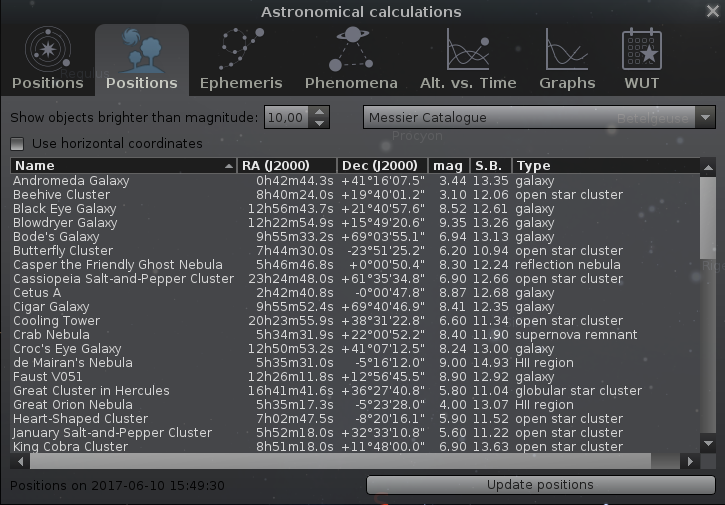
\includegraphics[width=0.68\textwidth]{astrocalc_dialog_positions2_tab}
\caption{Astronomical Calculations (AstroCalc): Celestial positions.}
\label{fig:gui:AstroCalc:CelestialPositions}
\end{figure}


\subsection{The Ephemeris Tab}
\label{sec:gui:AstroCalc:Ephemeris}

Select an object, start and end time, and compute an ephemeris (list of positions and magnitude evolving over time) for that object. The positions are marked in the sky with yellow circles (Figure~\ref{fig:gui:AstroCalc:Ephemeris}). When you click on a \emph{Show dates} and/or \emph{Show magnitudes} checkboxes, an orange circle indicates this date and/or magnitude. Double-clicking sets the respective date and brings object to focus. You can export the calculated ephemeris into CSV file. 

\begin{figure}[htbp]
\centering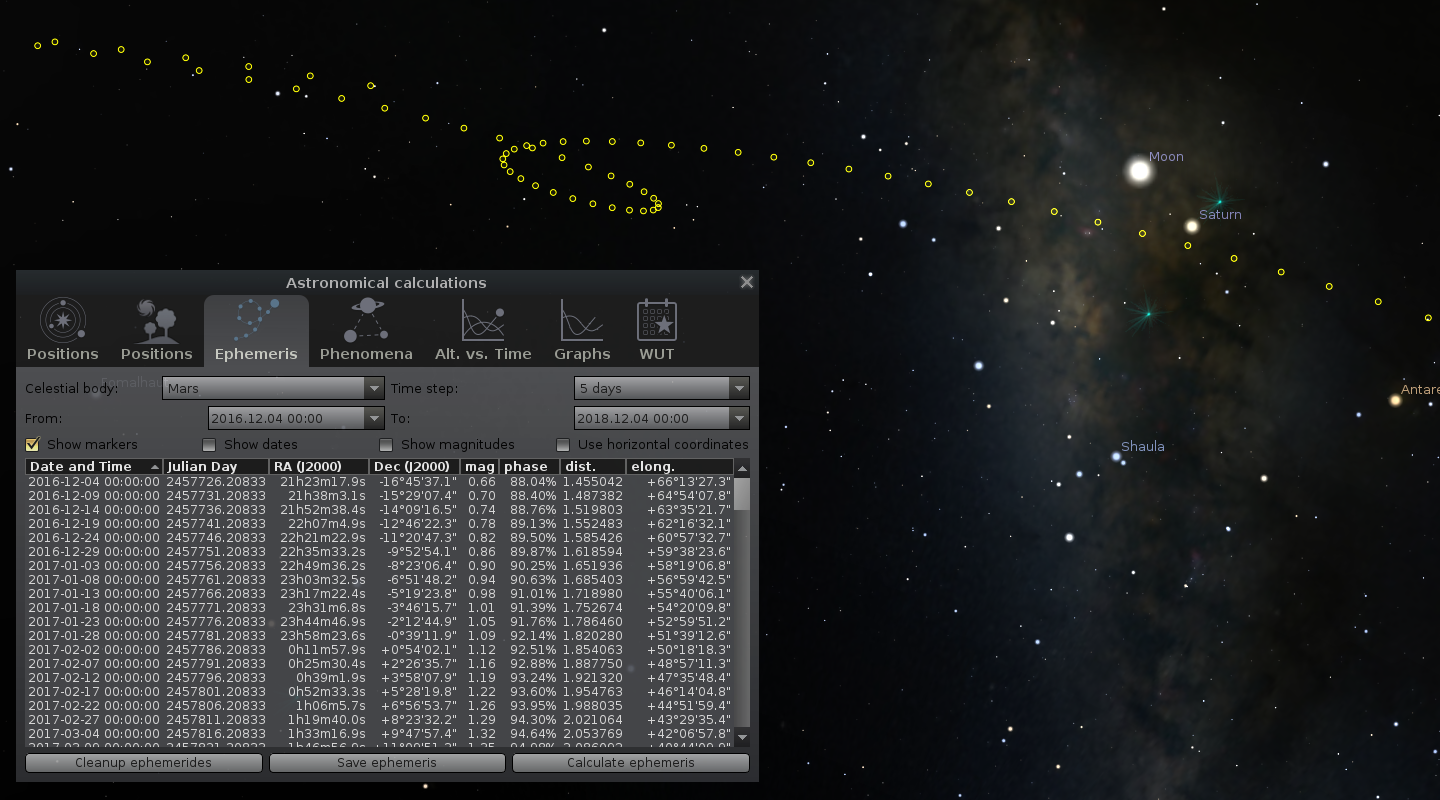
\includegraphics[width=\textwidth]{astrocalc_dialog_ephemeris_tab}
\caption{Astronomical Calculations (AstroCalc): Plot traces of planets.}
\label{fig:gui:AstroCalc:Ephemeris}
\end{figure}

Other interesting sight in this tool --- using horizontal coordinates for plot traces of the Solar system objects. For example you can get an analemma of the Sun for any location (Figure~\ref{fig:gui:AstroCalc:Ephemeris:Analemma}).

\begin{figure}[htbp]
\centering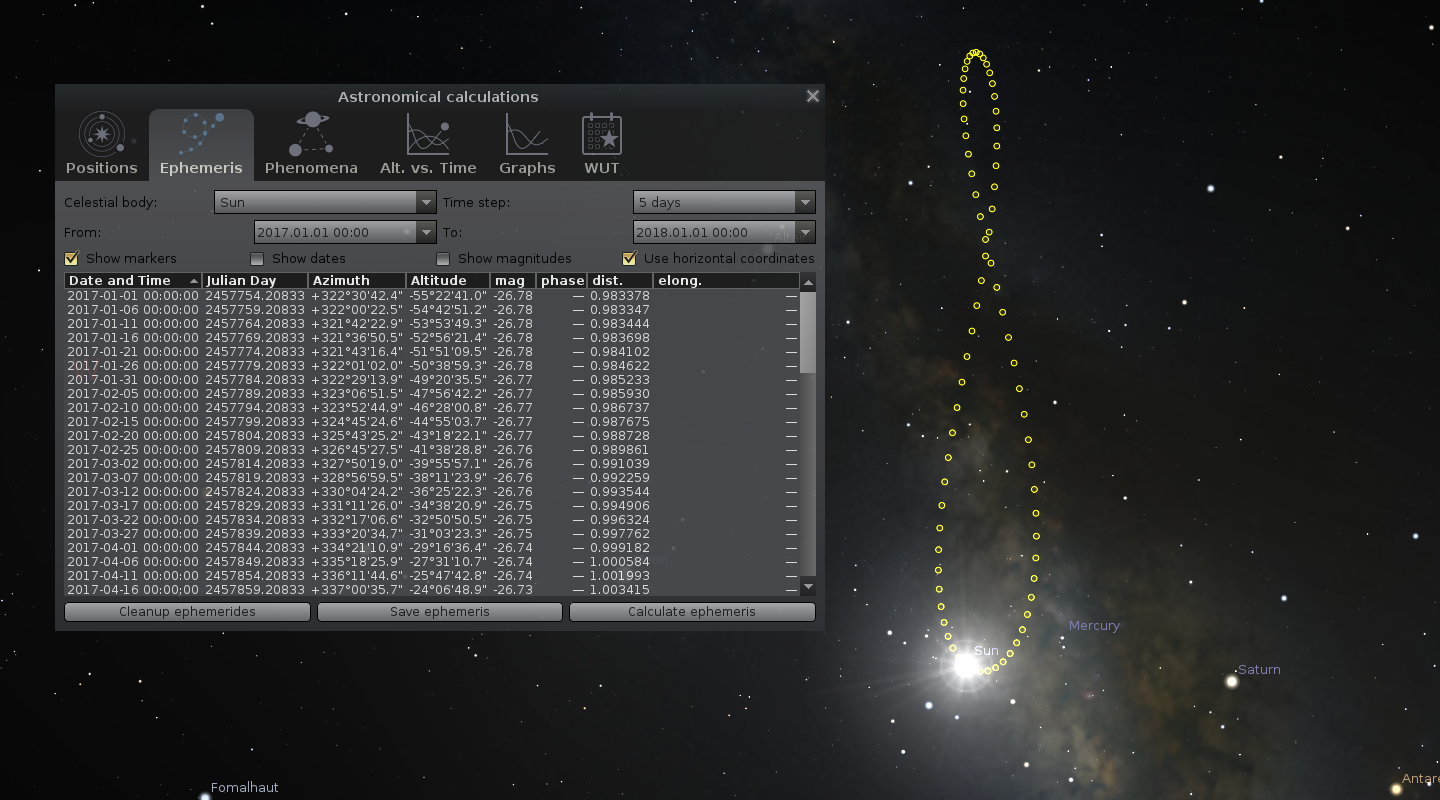
\includegraphics[width=\textwidth]{astrocalc_dialog_ephemeris_analemma}
\caption{Astronomical Calculations (AstroCalc): Analemma.}
\label{fig:gui:AstroCalc:Ephemeris:Analemma}
\end{figure}

\subsection{The Phenomena Tab}
\label{sec:gui:AstroCalc:Phenomena}

Compute phenomena like conjunctions, oppositions, occultations and eclipses (in special cases) between planetary objects (Figure~\ref{fig:gui:AstroCalc:Phenomena}). You can export the calculated phenomenae into CSV file.

\begin{figure}[htbp]
\centering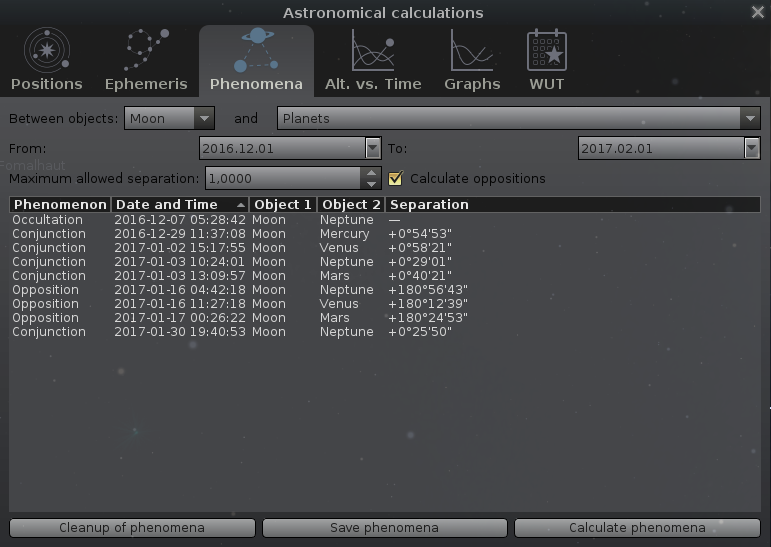
\includegraphics[width=0.68\textwidth]{astrocalc_dialog_phenomena_tab}
\caption{Astronomical Calculations (AstroCalc): Phenomena.}
\label{fig:gui:AstroCalc:Phenomena}
\end{figure}

\newpage
\subsection{The ``Altitude vs Time'' Tab}
\label{sec:gui:AstroCalc:AltVsTime}
  
Compute horizontal positions of object and draw it as a graph (Figure~\ref{fig:gui:AstroCalc:AltVsTime}).
    
\begin{figure}[htbp]
\centering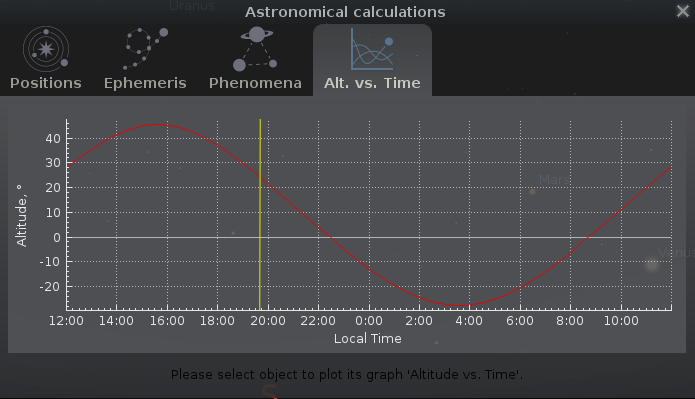
\includegraphics[width=0.68\textwidth]{astrocalc_dialog_altvstime_tab}
\caption{Astronomical Calculations (AstroCalc): Altitude vs Time.}
\label{fig:gui:AstroCalc:AltVsTime}
\end{figure}

\subsection{The Graphs Tab}
\label{sec:gui:AstroCalc:Graphs}
  
\newFeature{V0.16.0} Compute two functions by time for the current year and draw graphs for them on one desk (Figure~\ref{fig:gui:AstroCalc:Graphs}). This tool may be very helpful for educational and statistics purposes.
    
\begin{figure}[htbp]
\centering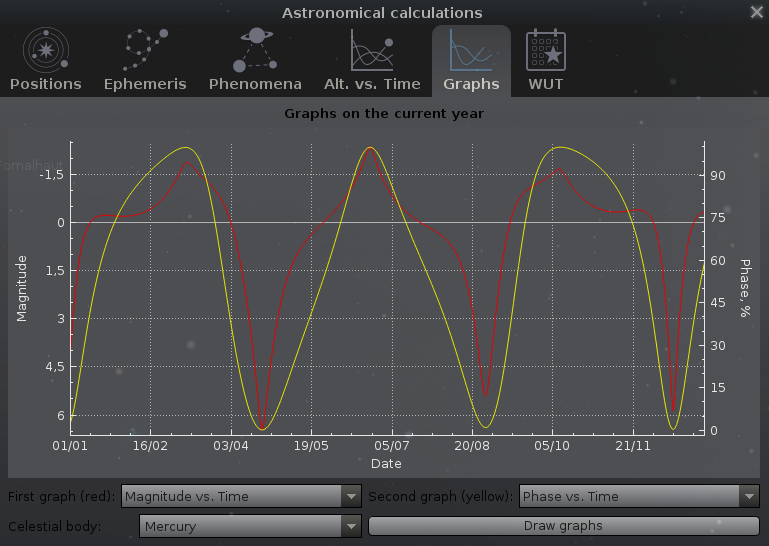
\includegraphics[width=0.68\textwidth]{astrocalc_dialog_graphs_tab}
\caption{Astronomical Calculations (AstroCalc): Graphs.}
\label{fig:gui:AstroCalc:Graphs}
\end{figure}

The list of possible functions for computations: \emph{Magnitude vs. Time}, \emph{Phase vs. Time}, \emph{Distance vs. Time}, \emph{Elongation vs. Time}, \emph{Angular size vs. Time} and \emph{Phase angle vs. Time}.

The idea for this tool has been obtained from the SkytechX planetarium\footnote{SkytechX --- \url{http://www.skytechx.eu/}}.

\subsection{The ``What's Up Tonight'' (WUT) Tab}
\label{sec:gui:AstroCalc:WUT}

\newFeature{V0.16.0} The ``What's Up Tonight'' (WUT) tool displays a list of objects that will be visible at night from any location, on any date. By default, the Date and Location are taken from the current settings in the Date and Time (see section~\ref{sec:gui:date}) and Location (see section~\ref{sec:gui:location}) windows.

\begin{figure}[htbp]
\centering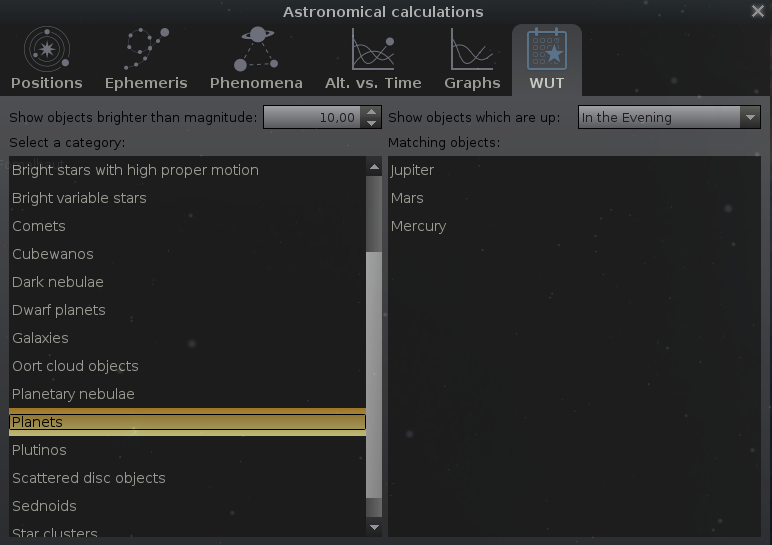
\includegraphics[width=0.68\textwidth]{astrocalc_dialog_wut_tab}
\caption{Astronomical Calculations (AstroCalc): What's Up Tonight (WUT).}
\label{fig:gui:AstroCalc:WUT}
\end{figure}

The objects are organized into type categories. Select an object type in the box labeled \emph{Select a Category}, and all objects of that type which are above the horizon on the selected night will be displayed in the box labeled \emph{Matching Objects}. For example, in the screenshot, the Planets category has been selected, and three planets which are up on the selected night are displayed (Jupiter, Mars and Mercury). 

By default, the WUT will display objects which are above the horizon between sunset and midnight (i.e. \emph{in the evening}). You can choose to show objects which are up between midnight and dawn (\emph{in the morning}), or between dusk and dawn (\emph{any time tonight}) using the combobox near the top of the window. You can also choose to see only those objects that are brighter than a magnitude by setting a minimum magnitude using the \emph{Show objects brighter than magnitude} spinbox. You may center the object in the sky map just by select of then.

This tool has been partially ported from the KStars planetarium\footnote{KStars --- \url{https://edu.kde.org/kstars/}}.
    
\section{Help Window}
\label{sec:gui:help}

\begin{figure}[htbp]
\centering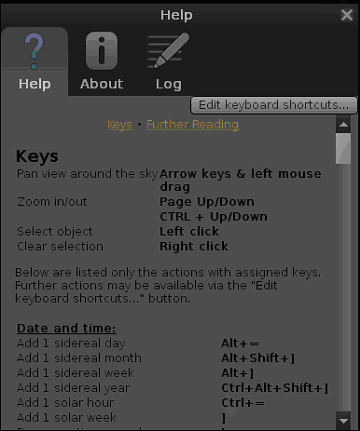
\includegraphics[width=0.68\textwidth]{help_dialog}
\caption{Help Window}
\label{fig:gui:help}
\end{figure}

\noindent The Help window lists all of Stellarium's keystrokes. Note that some
features are only available as keystrokes, so it's a good idea to have
a browse of the information in this window.

\subsection{Editing Keyboard Shortcuts}
\label{sec:gui:help:hotkeys}

You can edit the shortcut keys here. Each available function can be
configured with up to two key combinations. You may want to
reconfigure keys for example if you have a non-English keyboard layout
and some keys either do not work at all, or feel unintuitive for you,
or if you are familiar with other software and want to use the same
hotkeys for similar functions. Simply select the function and click
with the mouse into the edit field, then press your key of choice. If
the key has been taken already, a message will tell you.


\begin{figure}[htbp]
\centering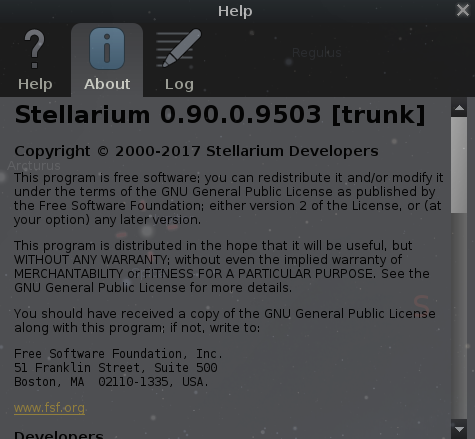
\includegraphics[width=0.68\textwidth]{help_dialog_about}
\caption{Help Window: About}
\label{fig:gui:help:about}
\end{figure}

The About Tab (Fig.~\ref{fig:gui:help:about}) shows version and licensing information, and a list
of people who helped to produce the program.

\begin{figure}[htbp]
\centering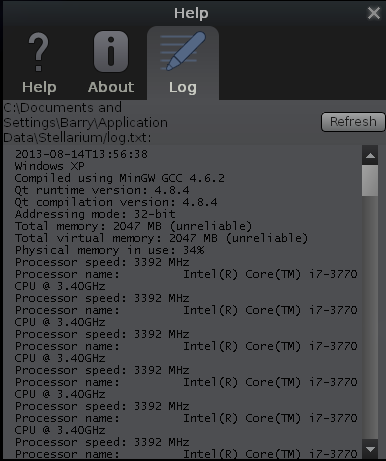
\includegraphics[width=0.68\textwidth]{help_dialog_log}
\caption{Help Window: Logfile}
\label{fig:gui:help:log}
\end{figure}

The Log Tab (Fig.~\ref{fig:gui:help:log}) shows messages like the loading confirmations carried out when
stellarium runs. It is useful to locate the files that stellarium writes
to your computer. The same information is written to  the file \file{log.txt} that you will
find in your user directory (see~\ref{sec:Directories}).




%%% Local Variables: 
%%% mode: latex
%%% TeX-master: "guide"
%%% End: 


%----------------------------------------------------------------------------------------
%	PART II
%----------------------------------------------------------------------------------------

\part{Advanced Use}

%----------------------------------------------------------------------------------------
%	CHAPTER 5 (Advanced Use)
%----------------------------------------------------------------------------------------
\chapterimage{chapter-t3-bg} % Chapter heading image

% Status info:
% M. Gates	2006-2009
% A. Wolf	2011-2015
% ArdWar	2012
% B. Gerdes	2013
% TODO insert further additions from wiki?
% Content OK for 0.15+.
% GZ: typo&grammar check 20160329

\chapter{Files and Directories}
\label{sec:FilesAndDirectories}

\section{Directories}
\label{sec:Directories}

Stellarium has many data files containing such things as star catalogue
data, nebula images, button icons, font files and configuration files.
When Stellarium looks for a file, it looks in two places. First, it
looks in the \emph{user directory} for the account which is running
Stellarium. If the file is not found there, Stellarium looks in the
\emph{installation directory}\footnote{The installation directory was
  referred to as the config root directory in previous versions of this
  guide}. Thus it is possible for Stellarium to be installed by an
administrative user and yet have a writable configuration file for
non-administrative users. Another benefit of this method is on
multi-user systems: Stellarium can be installed by the administrator,
and different users can maintain their own configuration and other files
in their personal user accounts.

In addition to the main search path, Stellarium saves some files in
other locations, for example screens shots and recorded scripts.

The locations of the user directory, installation directory,
\emph{screenshot save directory} and \emph{script save directory} vary
according to the operating system and installation options used. The
following sections describe the locations for various operating systems.

\subsection{Windows}
\label{sec:FilesAndDirectories:Windows}

\begin{description}
\item[installation directory] By default this is
  \file{C:\textbackslash{}Program\ Files\textbackslash{}Stellarium\textbackslash{}},
  although this can be adjusted during the installation process.
\item[user directory] This is the Stellarium sub-folder in the
  Application Data folder for the user account which is used to run
  Stellarium. Depending on the version of Windows and its configuration,
  this could be any of the following (each of these is tried, if it
  fails, the next in the list if tried).

\begin{commands}
%APPDATA%\Stellarium\
%USERPROFILE%\Stellarium\
%HOMEDRIVE%\%HOMEPATH%\Stellarium\
%HOME%\Stellarium\
Stellarium's installation directory
\end{commands}

Thus, on a typical Windows Vista/7/10 system with user ``Bob
Dobbs'', the user directory will be:

\begin{commands}
C:\Users\Bob Dobbs\AppData\Roaming\Stellarium\
\end{commands}

The user data directory is unfortunately hidden by default. To make it accessible in the Windows file
explorer, open an \program{Explorer} window and select \menu{Organize... > Folder and
search options}. Make sure folders marked as hidden are now 
displayed. Also, deselect the checkbox to ``hide known file name
endings''.\footnote{This is a very confusing default setting and in fact
  a security risk: Consider you receive an email with some file
  \file{funny.png.exe} attached. Your explorer displays this as
  \file{funny.png}. You double-click it, expecting to open some image
  browser with a funny image. However, you start some unknown program
  instead, and running this \file{.exe} executable program may turn
  out to be anything but funny!}

\item[screenshot save directory] Screenshots will be saved to the
  \file{Pictures/Stellarium} directory, although this can be changed with a command line option (see
  section~\ref{sec:CommandLineOptions}\footnote{Windows Vista users who do not run Stellarium with
    administrator privileges should adjust the shortcut in the start
    menu to specify a different directory for screenshots as the Desktop
    directory is not writable for normal programs. 
    Stellarium includes a GUI option to specify the screenshot
    directory.}).
\end{description}

\subsection{Mac OS X}
\label{sec:FilesAndDirectories:MacOSX}

\begin{description}
\item[installation directory] This is found inside the application
  bundle, \file{Stellarium.app}. See \emph{Inside Application
    Bundles}\footnote{\url{http://www.mactipsandtricks.com/articles/Wiley_HT_appBundles.lasso}}
  for more information.
\item[user directory] This is the sub-directory 
  \file{Library/Preferences/Stellarium/} (or \\
  \file{\textasciitilde{}/Library/Application\ Support/Stellarium} on
  newest versions of Mac OS X) of the user's home
  directory.
\item[screenshot save directory] Screenshots are saved to the user's
  Desktop.
\end{description}

\subsection{Linux}
\label{sec:FilesAndDirectories:Linux}

\begin{description}
\item[installation directory] This is in the
  \file{share/stellarium} sub-directory of the installation prefix,
  i.e., usually \file{/usr/share/stellarium} or
  \file{/usr/local/share/stellarium/}.
\item[user directory] This is the \file{.stellarium} sub-directory of
  user's home directory, i.e.,
  \file{\textasciitilde{}/.stellarium/}. This is a hidden folder, so
  if you are using a graphical file browser, you may want to change
  its settings to ``display hidden folders''.
\item[screenshot save directory] Screenshots are saved to the user's
  home directory.
\end{description}

\section{Directory Structure}
\label{sec:FilesAndDirectories:DirectoryStructure}

Within the \emph{installation directory} and \emph{user directory}
defined in section~\ref{sec:Directories}, files are arranged in the
following sub-directories.

\begin{description}
\item[\file{landscapes/}] contains data files and textures used for
  Stellarium's various landscapes. Each landscape has its own
  sub-directory. The name of this sub-directory is called the
  \emph{landscape ID}, which is used to specify the default landscape in
  the main configuration file, or in script commands.
\item[\file{skycultures/}] contains constellations, common star names and
  constellation artwork for Stellarium's many sky cultures. Each culture
  has its own sub-directory in the skycultures directory.
\item[\file{nebulae/}] contains data and image files for nebula textures.
  In the future Stellarium may be able to support multiple sets of nebula
  images and switch between them at runtime. This feature is not
  implemented for version~\StelVersion, although the directory structure is in
  place - each set of nebula textures has its own sub-directory in the
  nebulae directory.
  %% TODO: Update this if no longer valid.
\item[\file{stars/}] contains Stellarium's star catalogues. In the
  future Stellarium may be able to support multiple star catalogues
  and switch between them at runtime. This feature is not implemented
  for version~\StelVersion, although the directory structure is in
  place -- each star catalogue has its own sub-directory in the stars
  directory.
  %% TODO: Update this if no longer valid. 
\item[\file{data/}] contains miscellaneous data files including fonts,
  solar system data, city locations, etc.
\item[\file{textures/}] contains miscellaneous texture files, such as the
  graphics for the toolbar buttons, planet texture maps, etc.
\item[\file{ephem/}] (optional) may contain data files for planetary
  ephemerides DE430 and DE431 (see~\ref{sec:ExtraData:ephemerides}).
\end{description}

If any file exists in both the installation directory and user
directory, the version in the user directory will be used. Thus it is
possible to override settings which are part of the main Stellarium
installation by copying the relevant file to the user area and modifying
it there.

It is recommended to add new landscapes or sky cultures by creating the relevant files
and directories within the user directory, leaving the installation
directory unchanged. In this manner different users on a multi-user
system can customise Stellarium without affecting the other users. 

\section{The Main Configuration File}
\label{sec:ConfigurationFile}

The main configuration file is read each time Stellarium starts, and
settings such as the observer's location and display preferences are
taken from it. Ideally this mechanism should be totally transparent to
the user -- anything that is configurable should be configured ``in''
the program GUI. However, at time of writing Stellarium isn't quite
complete in this respect, despite improvements in each version. Some
settings, esp.\ color values for lines, grids, etc.\ can only be
changed by directly editing the configuration file.\footnote{Color
  values can be edited interactively by the Text User Interface plugin
  (see~\ref{sec:plugins:TextUserInterface}).} This section describes
some of the settings a user may wish to modify in this way, and how to
do it.

If the configuration file does not exist in the \emph{user directory}
when Stellarium is started (e.g., the first time the user starts the
program), one will be created with default values for all settings
(refer to section~\ref{sec:FilesAndDirectories} Files and
Directories for the location of the user directory on your operating
system). The name of the configuration file is
\file{config.ini}\footnote{It is possible to specify a different name
  for the main configuration file using the \texttt{-\/-config-file}
  command line option. See section~\ref{sec:CommandLineOptions} Command 
  Line Options for details.}.

The configuration file is a regular text file, so all you need to edit
it is a text editor like \program{Notepad} on Windows, \program{Text Edit} on
the Mac, or \program{nano}/\program{vi}/\program{gedit}/\program{emacs}/\program{leafpad} etc.\ on Linux.

%The following sub-sections contain details on how to make commonly used
%modifications to the configuration file. 
A complete list of configuration file options and values may be found
in appendix~\ref{sec:config.ini} Configuration File.



\section{Getting Extra Data}
\label{sec:ExtraData}

Stellarium is packaged with over 600 thousand stars in the normal
program download, but much larger star catalogues may be downloaded
in the \emph{Tools} tab of the \emph{Configuration} dialog.


\subsection{Alternative Planet Ephemerides: DE430, DE431}
\label{sec:ExtraData:ephemerides}

\newFeature{0.15}
By default, Stellarium uses the \indexterm{VSOP87} planetary theory,
an analytical solution which is able to deliver planetary positions
for any input date. However, its use is recommended only for the year
range $-4000\ldots+8000$. Outside this range, it seems to be usable
for a few more millennia without too great errors, but with degrading accuracy. 

Since V0.15 you can install extra data files which allow access to the
numerical integration runs \indexterm{DE430} and \indexterm{DE431}
from NASA's Jet Propulsion Laboratory (JPL). The data files have to be
downloaded separately, and most users will likely not need them. DE430
provides highly accurate data for the years $+1550\ldots+2650$, while
DE431 covers years $-13000\ldots+17000$, which allows e.g.\ 
archaeoastronomical research on Mesolithic landscapes. Outside these
year ranges, positional computation falls back to VSOP87.

The integration of this feature is still experimental. As of V0.15,
solar eclipses in antiquity seem to be slightly off. Please use JPL
Horizon for quotable results.
% GZ TODO: FIX THAT ASAP!! 

To enable use of these data, download the files from
JPL\footnote{\url{ftp://ssd.jpl.nasa.gov/pub/eph/planets/Linux/}. (Also
  download from this directory if you are not running Linux!)}:

\begin{tabular}{ccc}
\toprule
\emph{Ephemeris}&\emph{Filename}& \emph{MD5 hash}\\\midrule
DE430& \file{linux\_p1550p2650.430} &\texttt{707c4262533d52d59abaaaa5e69c5738}\\
DE431& \file{lnxm13000p17000.431}   &\texttt{fad0f432ae18c330f9e14915fbf8960a}\\\bottomrule
\end{tabular}


The files can be placed in a folder named \file{ephem} inside either
the \emph{installation directory} or the \emph{user directory}
(see \ref{sec:FilesAndDirectories:DirectoryStructure}). Alternatively,
if you have them already stored elsewhere, you may add the path to
\file{config.ini} like:

\begin{configfile}
[astro]
de430_path = C:/Astrodata/JPL_DE43x/linux_p1550p2650.430
de431_path = C:/Astrodata/JPL_DE43x/lnxm13000p17000.431
\end{configfile}

For fast access avoid storing them on a network drive or USB pendrive!

You activate use of either ephemeris in the configuration panel
(\key{F2}). If you activate both, preference will be given for DE430
if the simulation time allows it. Outside of the valid times, VSOP87
will always be used.

\paragraph{Acknowledgement}
The optional use of DE430/431 has been supported by the ESA Summer of
Code 2015 initiative.


\chapter{Command Line Options}
%\label{command-line-options}
\label{sec:CommandLineOptions}

Stellarium's behaviour can be modified by providing parameters to the
program when it is called via the command line. See table for a full list:

\begin{longtabu} to \textwidth {l|l|X}\toprule
\emph{Option}         & \emph{Option Parameter} & \emph{Description}\\\midrule
-\/-help or -h        & {[}none{]}       & Print a quick command line help message, and exit. \\\midrule
-\/-version or -v     & {[}none{]}       & Print the program name and version information, and exit. \\\midrule
-\/-config-file or -c & config file name & Specify the configuration file name. The default value is \file{config.ini}.

The parameter can be a full path (which will be used verbatim) or a partial path.

Partial paths will be searched for inside the regular search paths
unless they start with a ``\file{.}'', which may be used to explicitly
specify a file in the current directory or similar.

For example, using the option \texttt{-c\ my\_config.ini} would resolve to the file 
\file{\textless{}user\ directory\textgreater{}/my\_config.ini} whereas 
\file{-c\ ./my\_config.ini} can be used to explicitly say the file
\file{my\_config.ini} in the current working directory.\\\midrule
-\/-restore-defaults &  [none]    & Stellarium will start with the default configuration. 
                                    Note: The old configuration file will be overwritten. \\\midrule
-\/-user-dir         & path       & Specify the user data directory. \\\midrule
-\/-screenshot-dir   & path       & Specify the directory to which screenshots will be saved. \\\midrule
-\/-full-screen      & yes or no  & Over-rides the full screen setting in the config file. \\\midrule
-\/-home-planet      & planet     & Specify observer planet (English name). \\\midrule
-\/-altitude         & altitude   & Specify observer altitude in meters. \\\midrule
-\/-longitude        & longitude  & Specify latitude, e.g. +53d58'16.65" \\\midrule
-\/-latitude         & latitude   & Specify longitude, e.g. -1d4'27.48" \\\midrule
-\/-list-landscapes  & {[}none{]} & Print a list of available landscape IDs and exit. \\\midrule
-\/-landscape        & landscape ID & Start using landscape whose ID matches the passed parameter (dir name of landscape). \\\midrule
-\/-sky-date         & date       & The initial date in \texttt{yyyymmdd} format. \\\midrule
-\/-sky-time         & time       & The initial time in \texttt{hh:mm:ss} format. \\\midrule
-\/-startup-script   & script name & The name of a script to run after the program has started. \\\midrule
-\/-fov              & angle      & The initial field of view in degrees. \\\midrule
-\/-projection-type  & ptype      & The initial projection type (e.g. \texttt{perspective}). \\\midrule
-\/-spout  or -S     & all or sky & Act as Spout sender (See section \ref{sec:CommandLineOptions:Special:Spout}).%
                                    \footnote{On Windows only}\footnote{This function requires running in OpenGL mode.}\\\midrule
-\/-spout-name       & name       & Use \texttt{name} as name of the Spout sender. Default name: \texttt{Stellarium}.\footnotemark[1]\\\midrule									
-\/-dump-opengl-details or -d     & {[}none{]} & Dump information about OpenGL support to logfile. 
                                                 Use this is you have graphics problems and want to send a bug report. \\\midrule
-\/-angle-mode or -a & {[}none{]} & Use ANGLE as OpenGL ES2 rendering engine (autodetect Direct3D version).\footnotemark[1]\\\midrule
-\/-angle-d3d9 or -9 & {[}none{]} & Force use Direct3D 9 for ANGLE OpenGL ES2 rendering engine.\footnotemark[1]\\\midrule
-\/-angle-d3d11      & {[}none{]} & Force use Direct3D 11 for ANGLE OpenGL ES2 rendering engine.\footnotemark[1]\\\midrule
-\/-angle-warp       & {[}none{]} & Force use the Direct3D 11 software rasterizer for ANGLE OpenGL ES2 rendering engine.\footnotemark[1]\\\midrule
-\/-mesa-mode or -m  & {[}none{]} & Use MESA as software OpenGL rendering engine.\footnotemark[1]\\\midrule
-\/-safe-mode or -s  & {[}none{]} & Synonymous to -\/-mesa-mode.\footnotemark[1]\\\midrule
-\/-fix-text or -t   & {[}none{]} & Alternative way of creating the Info text, required on some systems.\footnote{E.g., Raspberry Pi 2 with Raspbian Jessie and VC4 drivers from February 2016. A driver update which makes this unnecessary should be available later in 2016.}\\\bottomrule
\end{longtabu}

\noindent \newFeature{0.15} If you want to avoid adding the same
switch every time when you start Stellarium from the command line, you
can also set an environment variable \file{STEL\_OPTS} with your
default options. 

\section{Examples}
\label{sec:CommandLineOptions:Examples}

\begin{itemize}
\item To start Stellarium using the configuration file,
  \file{configuration\_one.ini} situated in the user directory (use either of
  these):

\begin{commands}
stellarium --config-file=configuration_one.ini
stellarium -c configuration_one.ini
\end{commands}

\item To list the available landscapes, and then start using the
  landscape with the ID ``ocean''
\begin{commands}
stellarium --list-landscapes 
stellarium --landscape=ocean
\end{commands}
\end{itemize}

%% GZ found in 2015:
\noindent Note that console output (like \command{-\/-list-landscapes}) on Windows is not possible. 

\section{Special Options}
\label{sec:CommandLineOptions:Special}
\subsection{Spout}\newFeature{0.15.1} 
\label{sec:CommandLineOptions:Special:Spout}
Apart from stand-alone use, Stellarium can be used as multimedia source in larger installations, in museums or science exhibitions. 
\program{Spout}\footnote{\url{http://spout.zeal.co/}} is a technology which enables use of Stellarium's 
output window as texture in DirectX applications on Windows. Simply start Stellarium with 
the \texttt{-\/-spout=sky} command line option. (Currently \program{Spout} output is limited to the main window 
without GUI panels, but this may change in future versions.) 
Your master application must obviously embed a \program{Spout} receiver. 
The default name of the \program{Spout} sender is \texttt{Stellarium}. If you need more than one instance of Stellarium acting as source, 
you can use option \texttt{-\/-spout-name=StelSpout2} in addition to create another \program{Spout} sender without a name conflict. 
In such cases, it may be useful to also have separate user data directories and use option \texttt{-\/-user-dir}. 

This mode does not work in ANGLE mode and requires modern graphics hardware with the \texttt{WGL\_NV\_DX\_interop} 
driver extension running in OpenGL mode. Some NVidia GPUs work without this extension listed explicitly. 
On a notebook with NVidia Optimus technology, make sure to launch Stellarium on the NVidia hardware. 
For permanent setting, use the NVidia configuration dialog to configure Stellarium explicitly to run always on the NVidia card.

%%% Local Variables: 
%%% mode: latex
%%% TeX-master: "guide"
%%% End: 


%% GZ I propose to  replace the old chapter with course notes I have developed in late 2015. To get the old version, activate next line instead.
%
\chapter{Landscapes}\label{customising-landscapes}
\label{ch:landscapes}

Stellarium comes with a selection of panorama landscapes which try to
link the sky with the observer's surrounding and thus create a more
immersive feeling.  It is possible to create your own landscapes for
Stellarium, this is described in
section~\ref{sec:landscapes:customizing}. 

\section{Landscape Types}
\label{sec:landscapes:types}


There are four types of landscape:

\begin{itemize}
\item
  \textbf{Polygonal Method} Using a text file with azimuths/altitudes.
\item
  \textbf{Single Fish-eye Method} Using a fish-eye panorama image.
\item
  \textbf{Single Spherical Method} Using a spherical panorama image.
\item
  \textbf{Multiple Image Method} (\textbf{also called ``old style''
  landscapes}) Using a series of images split from a 360$\degree$ ``strip''
  panorama image + a ground image.
\end{itemize}

Each landscape has its own sub-directory in
\texttt{\textless{}user\ directory\textgreater{}/landscapes} or
\texttt{\textless{}installation\ directory\textgreater{}/landscapes}.
The name of the sub-directory is called the \emph{landscape ID}. The
sub-directory must contain a file called \texttt{landscape.ini} which
describes the landscape type, texture filenames and other data. Texture
files for a landscape should by put in the same directory as the
\texttt{landscape.ini} file, although if they are not found there they
will be searched for in the \texttt{.../textures} directory, allowing
shared files for common textures such as the generic fog texture.

For example, the \emph{Moon} landscape that is provided with Stellarium
has the following files:

\texttt{.../landscapes/moon/landscape.ini}\\
\texttt{.../landscapes/moon/apollo17.png}

The \texttt{landscape.ini} file must contain a section called
\texttt{{[}landscape{]}}, which contains the details necessary to render
the landscape (which vary, depending on the type of the landscape).

There is also an optional \texttt{{[}location{]}} section which is used
to tell Stellarium where the landscape is in the solar system. If the
\texttt{{[}location{]}} section exists, Stellarium can automatically
adjust the location and observing conditions of the observer to match
the landscape.

\subsection{Polygonal Landscape}\label{polygonal-line-method}

This is the technically simplest of the landscapes, but may be used to
describe accurately measured horizon lines. The file that encodes
horizon altitudes can also be used in all other landscape types. If
present there, it will be used to define object visibility (instead of
the opacity of the landscape photo textures) and, if
\texttt{horizon\_line\_color} is defined, will be plotted.

There is a small caveat: Sometimes, there may appear vertical lines from
some corners towards the zenith or the mathematical horizon, e.g. if
there is a vertex including azimuth 0 or 180. If this irritates you,
just offset this azimuth minimally (e.g., 180.00001).

The \texttt{landscape.ini} file for a polygonal type landscape looks
like this (this example is based on the Geneve landscape which was
borrowed from Cartes du Ciel and comes with Stellarium):

\begin{config}
\texttt{{[}landscape{]}}\\
\texttt{name~=~Geneve}\\
\texttt{type~=~polygonal}\\
\texttt{author~=~Georg~Zotti;~Horizon~definition~by~Patrick~Chevalley}\\
\texttt{description~=~Horizon~line~of~Geneve.~Demonstrates~compatibility~with~horizon~descriptions~from~~Cartes~du~Ciel.}\\
\texttt{polygonal\_horizon\_list~=~horizon\_Geneve.txt}\\
\texttt{polygonal\_angle\_rotatez~=~0}\\
\texttt{ground\_color~=~.15,.45,.45}\\
\texttt{horizon\_line\_color~=~~.75,.45,.45}
\end{config}

Where:

\begin{itemize}
\item
  \textbf{name} is what appears in the landscape tab of the
  configuration window.
\item
  \textbf{type} identifies the method used for this landscape.
  ``polygonal'' in this case.
\item
  \textbf{author} lists the author(s) responsible for images and
  composition.
\item
  \textbf{description} gives a short description visible in the
  selection panel. The text will be superseded by optional
  \texttt{description.\&lt;lang\&gt;.utf8} files.
\item
  \textbf{polygonal\_horizon\_list} is the name of the horizon data file
  for this landscape.
\item
  \textbf{polygonal\_horizon\_list\_mode} (optional) the two first
  columns in the list are numbers: azimuth and altitude or zenith
  distance, in either degrees or radians or gradians(gon). The value
  must be one of
  \texttt{azDeg\_altDeg\textbar{}azDeg\_zdDeg\textbar{}azRad\_altRad\textbar{}azRad\_zdRad\textbar{}azGrad\_altGrad\textbar{}azGrad\_zdGrad}.
  Default: azDeg\_altDeg
\item
  \textbf{polygonal\_angle\_rotatez} (optional, default=0) Angle
  (degrees) to adjust azimuth. This may be used to apply a (usually)
  small offset rotation, e.g. when you have measured the horizon in a
  grid-based coordinate system like UTM and have to compensate for the
  meridian convergence.
\item
  \textbf{ground\_color} (optional, default=``0,0,0'', i.e., black)
  Color for the area below the horizon line. Each R,G,B component is a
  float within 0..1.
\item
  \textbf{horizon\_line\_color} (optional, default: invisible) used to
  draw a polygonal horizon line. Each R,G,B component is a float within
  0..1.
\item
  \textbf{minimal\_brightness} (optional, default=-1, i.e. use preset
  landscape/minimal\_brightness from global \texttt{config.ini}) Some
  minimum brightness to keep landscape visible.
\item
  \textbf{minimal\_altitude} (optional, default=-2) Some sky elements,
  e.g. stars, are not drawn below this altitude. Under certain
  circumstances you may want to specify something else here. (since
  V0.14)
\end{itemize}

\subsection{Single Fish-eye Landscape}\label{single-fish-eye-method}

The \emph{Trees} landscape that is provided with Stellarium is an
example of the single fish-eye method, and provides a good illustration.
The centre of the image is the spot directly above the observer (the
zenith). The point below the observer (the nadir) becomes a circle that
just touches the edges of the image. The remaining areas of the image
(the corners outside the circle) are not used.

The image file should be saved in PNG format with alpha transparency.
Wherever the image is transparent is where Stellarium will render the
sky.

The \texttt{landscape.ini} file for a fish-eye type landscape looks like
this (this example is based on the Trees landscape which comes with
Stellarium):

\begin{config}
\texttt{{[}landscape{]}}\\
\texttt{name~=~Trees}\\
\texttt{type~=~fisheye}\\
\texttt{author~=~Robert~Spearman.~Light~pollution~image:~Georg~Zotti}\\
\texttt{description~=~Trees~in~Greenlake~Park,~Seattle}\\
\texttt{maptex~=~trees\_512.png}\\
\texttt{maptex\_illum~=~trees\_illum\_512.png}\\
\texttt{maptex\_fog~=~trees\_fog\_512.png}\\
\texttt{texturefov~=~210}\\
\texttt{angle\_rotatez~=~17}\\
\texttt{tesselate\_rows~=~28}\\
\texttt{tesselate\_cols~=~60}
\end{config}

Where:

\begin{itemize}
\item
  \textbf{name} is what appears in the landscape tab of the
  configuration window.
\item
  \textbf{type} identifies the method used for this landscape.
  ``fisheye'' in this case.
\item
  \textbf{author} lists the author(s) responsible for images and
  composition.
\item
  \textbf{description} gives a short description visible in the
  selection panel. The text will be superseded by optional
  \texttt{description.\&lt;lang\&gt;.utf8} files.
\item
  \textbf{maptex} is the name of the image file for this landscape.
\item
  \textbf{maptex\_fog} (optional) is the name of the fog image file for
  this landscape.
\item
  \textbf{maptex\_illum} (optional) is the name of the nocturnal
  illumination/light pollution image file for this landscape.
\item
  \textbf{texturefov} is the field of view that the image covers in
  degrees.
\item
  \textbf{angle\_rotatez} (optional) Angle (degrees) to adjust azimuth.
\item
  \textbf{tesselate\_rows} (optional, default=20) If straight edges in
  your landscape appear broken, try increasing.
\item
  \textbf{tesselate\_cols} (optional, default=40) If straight edges in
  your landscape appear broken, try increasing.
\item
  \textbf{polygonal\_horizon\_list} (optional) is the name of the
  (measured) horizon data file for this landscape.
\item
  \textbf{polygonal\_horizon\_list\_mode} (optional) the two first
  columns in the list are numbers: azimuth and altitude or zenith
  distance, in either degrees or radians or gradians(gon). The value
  must be one of
  \texttt{azDeg\_altDeg \textbar{} azDeg\_zdDeg \textbar{} azRad\_altRad \textbar{} azRad\_zdRad \textbar{} azGrad\_altGrad \textbar{} azGrad\_zdGrad}.
  Default: \texttt{azDeg\_altDeg}
\item
  \textbf{polygonal\_angle\_rotatez} (optional, default=0) Angle
  (degrees) to adjust azimuth. This may be used to apply a (usually)
  small offset rotation, e.g. when you have measured the horizon in a
  grid-based coordinate system like UTM and have to compensate for the
  meridian convergence.
\item
  \textbf{horizon\_line\_color} (optional, default: invisible) used to
  draw a polygonal horizon line.
\item
  \textbf{minimal\_brightness} (optional, default=-1, i.e. use preset
  landscape/minimal\_brightness from global \texttt{config.ini}) Some
  minimum brightness to keep landscape visible.
\item
  \textbf{minimal\_altitude} (optional, default=-2) Some sky elements,
  e.g. stars, are not drawn below this altitude. Under certain
  circumstances you may want to specify something else here. (since
  V0.14)
\end{itemize}

\subsection{Single Panorama Landscape}\label{single-panorama-method}

This method uses a more usual type of panorama - the kind which is
produced directly from software such as \emph{autostitch} or Hugin
(http://hugin.sourceforge.net/). The panorama file should be copied into
the
\texttt{\textless{}config\ root\textgreater{}/landscapes/\textless{}landscape\_id\textgreater{}}
directory, and a \texttt{landscape.ini} file created. The \emph{Moon}
landscape which comes with Stellarium provides a minimal example of the
contents of a landscape.ini file for a spherical type landscape:

\begin{config}
\texttt{{[}landscape{]}}\\
\texttt{name~=~Moon}\\
\texttt{type~=~spherical}\\
\texttt{maptex~=~apollo17.png}
\end{config}

A more elaborate example is found with the \emph{Grossmugl} landscape:

\begin{config}
\texttt{{[}landscape{]}}\\
\texttt{name~=~Grossmugl}\\
\texttt{type~=~spherical}\\
\texttt{author~=~Guenther~Wuchterl,~Kuffner-Sternwarte.at;~Lightscape:~Georg~Zotti}\\
\texttt{description~=~Field~near~Leeberg,~Grossmugl~(Riesentumulus),~Austria~-~Primary~Observing~Spot~of~the~Grossmugl~Starlight~Oasis~-~}\href{http://starlightoasis.org}{\texttt{http://starlightoasis.org}}\\
\texttt{maptex~=~grossmugl\_leeberg\_crop11.25.png}\\
\texttt{maptex\_top=11.25~}\\
\texttt{maptex\_fog~=~grossmugl\_leeberg\_fog\_crop22.5.png}\\
\texttt{maptex\_fog\_top~=~22.5}\\
\texttt{maptex\_fog\_bottom~=~-22.5}\\
\texttt{maptex\_illum~=~grossmugl\_leeberg\_illum\_crop0.png}\\
\texttt{maptex\_illum\_bottom~=~0}\\
\texttt{angle\_rotatez=-89.1}\\
\texttt{minimal\_brightness~=~0.0075}\\
\texttt{polygonal\_horizon\_list~=~horizon\_grossmugl.txt}\\
\texttt{polygonal\_angle\_rotatez=0}\\
\texttt{horizon\_line\_color~=~~.75,.45,.45}\\
\texttt{minimal\_altitude~=~-1}
\end{config}

Where:

\begin{itemize}
\item
  \textbf{name} is what appears in the landscape tab of the
  configuration window.
\item
  \textbf{type} identifies the method used for this landscape.
  ``spherical'' in this case.
\item
  \textbf{author} lists the author(s) responsible for images and
  composition.
\item
  \textbf{description} gives a short description visible in the
  selection panel. The text will be superseded by optional
  \texttt{description.\&lt;lang\&gt;.utf8} files.
\item
  \textbf{maptex} is the name of the image file for this landscape.
\item
  \textbf{maptex\_top} (optional; default=90) is the altitude angle of
  the top edge.
\item
  \textbf{maptex\_bottom} (optional; default=-90) is the altitude angle
  of the bottom edge. Usually you will not require this, or else there
  will be a hole at your feet. ;-)
\item
  \textbf{maptex\_fog} (optional; default: no fog) is the name of the
  fog image file for this landscape.
\item
  \textbf{maptex\_fog\_top} (optional; default=90) is the altitude angle
  of the top edge of the fog texture. Useful to crop away parts of the
  image to conserve texture memory.
\item
  \textbf{maptex\_fog\_bottom} (optional; default=-90) is the altitude
  angle of the bottom edge.
\item
  \textbf{maptex\_illum} (optional; default: no illumination layer) is
  the name of the nocturnal illumination/light pollution image file for
  this landscape.
\item
  \textbf{maptex\_illum\_top} (optional; default=90) is the altitude
  angle of the top edge, if you have light pollution only close to the
  horizon.
\item
  \textbf{maptex\_illum\_bottom} (optional; default=-90) is the altitude
  angle of the bottom edge.
\item
  \textbf{angle\_rotatez} (optional, default=0) Angle (degrees) to
  adjust azimuth. If 0, the left/right edge is due east.
\item
  \textbf{tesselate\_rows} (optional, default=20) If straight edges in
  your landscape appear broken, try increasing. This is the number of
  rows for the maptex. Fog and illumination textures will have a similar
  vertical angle.
\item
  \textbf{tesselate\_cols} (optional, default=40) If straight edges in
  your landscape appear broken, try increasing.
\item
  \textbf{polygonal\_horizon\_list} (optional) is the name of the
  (measured) horizon data file for this landscape. Can be used to query
  horizon transparency (for accurate object rising/setting times)
\item
  \textbf{polygonal\_horizon\_list\_mode} (optional) the two first
  columns in the list are numbers: azimuth and altitude or zenith
  distance, in either degrees or radians or gradians(gon). The value
  must be one of
  \texttt{azDeg\_altDeg\textbar{}azDeg\_zdDeg\textbar{}azRad\_altRad\textbar{}azRad\_zdRad\textbar{}azGrad\_altGrad\textbar{}azGrad\_zdGrad}.
  Default: \texttt{azDeg\_altDeg}
\item
  \textbf{polygonal\_angle\_rotatez} (optional, default=0) Angle
  (degrees) to adjust azimuth. This may be used to apply a (usually)
  small offset rotation, e.g. when you have measured the horizon in a
  grid-based coordinate system like UTM and have to compensate for the
  meridian convergence.
\item
  \textbf{horizon\_line\_color} (optional, default: invisible) used to
  draw a polygonal horizon line.
\item
  \textbf{minimal\_brightness} (optional, default=-1, i.e. use preset
  landscape/minimal\_brightness from global config.ini) Some minimum
  brightness to keep landscape visible.
\item
  \textbf{minimal\_altitude} (optional, default=-2) Some sky elements,
  e.g. stars, are not drawn below this altitude. Under certain
  circumstances (e.g. for space station panoramas where you may have sky
  below your feet, or for deep valleys/high mountains for efficiency,
  you may want to specify something else here. (since V0.14)
\end{itemize}

To save texture memory, since V0.13 you can trim away the transparent
sky and define the angle \textbf{maptex\_top}. Likewise,
\textbf{fogtex\_top}, \textbf{fogtex\_bottom},
\textbf{maptex\_illum\_top} and \textbf{maptex\_illum\_top}. You should
then stretch the texture to a full power of 2, like 4096x1024. The
easiest method to create perfectly aligned fog and illumination layers
is with an image editor that supports layers like the GIMP or Photoshop.
Fog and Light images should have black background.

\subsection{Multiple Image Landscape}\label{multiple-image-method}

The multiple image method works by having a 360 panorama of the horizon
(without wasting too much texture memory with the sky) split into a
number of smaller ``side textures'', and a separate ``ground texture''.
This has the advantage over the single image method that the detail
level of the horizon can be increased further without ending up with a
single very large image file, so this is usable for either very
high-resolution panoramas or for older hardware. The ground texture can
be a lower resolution than the panorama images. Memory usage may be more
efficient because there are no unused texture parts like the corners of
the texture file in the fish-eye method. It is even possible to repeat
the horizon several times (for purely decorative purpose). The side
textures are indeed mapped onto curved (spherical ring or cylinder)
walls, not flat sides as shown here.

\begin{figure}[h]
\centering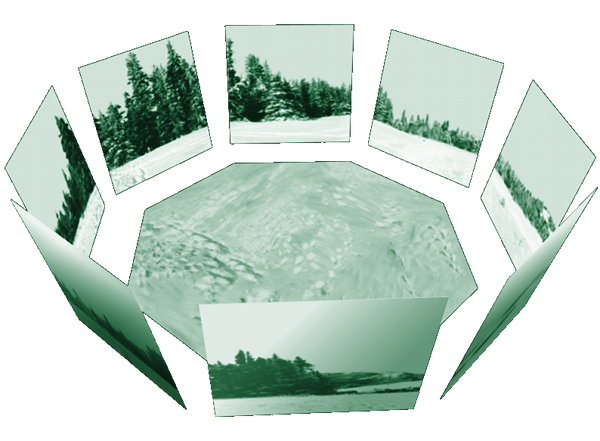
\includegraphics[scale=0.7]{faq_landscape}
%\caption{Figure caption}
\end{figure}

On the negative side, it is more difficult to create this type of
landscape - merging the ground texture with the side textures can prove
tricky. The contents of the \texttt{landscape.ini} file for this
landscape type is also somewhat more complicated than for other
landscape types. Here is the \texttt{landscape.ini} file which describes
the Guereins landscape:

\begin{config}
\texttt{{[}landscape{]}}\\
\texttt{name~=~Guereins}\\
\texttt{type~=~old\_style}\\
\texttt{author~=~Fabien~Chéreau}\\
\texttt{description~=~Guéreins~is~a~small~french~village...}\\
\texttt{nbsidetex~=~8}\\
\texttt{tex0~=~guereins4.png}\\
\texttt{tex1~=~guereins5.png}\\
\texttt{tex2~=~guereins6.png}\\
\texttt{tex3~=~guereins7.png}\\
\texttt{tex4~=~guereins8.png}\\
\texttt{light4~=~guereins8-lgt.png}\\
\texttt{tex5~=~guereins1.png}\\
\texttt{tex6~=~guereins2.png}\\
\texttt{tex7~=~guereins3.png}\\
\texttt{nbside~=~8}\\
\texttt{side0~=~tex0:0:0.005:1:1}\\
\texttt{side1~=~tex1:0:0.005:1:1}\\
\texttt{side2~=~tex2:0:0.005:1:1}\\
\texttt{side3~=~tex3:0:0.005:1:1}\\
\texttt{side4~=~tex4:0:0.005:1:1}\\
\texttt{side5~=~tex5:0:0.005:1:1}\\
\texttt{side6~=~tex6:0:0.005:1:1}\\
\texttt{side7~=~tex7:0:0.005:1:1}\\
\texttt{groundtex~=~guereinsb.png}\\
\texttt{fogtex~=~fog.png}\\
\texttt{nb\_decor\_repeat~=~1}\\
\texttt{decor\_alt\_angle~=~40}\\
\texttt{decor\_angle\_shift~=~-22}\\
\texttt{decor\_angle\_rotatez~=~0}\\
\texttt{ground\_angle\_shift~=~-22}\\
\texttt{ground\_angle\_rotatez~=~45}\\
\texttt{fog\_alt\_angle~=~20}\\
\texttt{fog\_angle\_shift~=~-3}\\
\texttt{draw\_ground\_first~=~1}
\end{config}

Where:

\begin{itemize}
\item
  \textbf{name} is the name that will appear in the landscape tab of the
  configuration window for this landscape
\item
  \textbf{type} should be ``old\_style'' for the multiple image method.
\item
  \textbf{author} lists the author(s) responsible for images and
  composition.
\item
  \textbf{description} gives a short description visible in the
  selection panel. The text will be superseded by optional
  description..utf8 files.
\item
  \textbf{nbsidetex} is the number of side textures for the landscape.
\item
  \textbf{tex0 ... tex} are the side texture file names. These should
  exist in the \texttt{.../textures/landscapes} directory in PNG format.
\item
  \textbf{light0 ... light} are optional textures. If they exist, they
  are used as overlays on top of the respective
  tex\textless{}...\textgreater{} files and represent nocturnal
  illumination, e.g. street lamps, lit windows, red dots on towers, sky
  glow by city light pollution, ... Empty panels don't have to exist. If
  you need your light pollution higher in the sky, you must use a
  spherical or fisheye landscape. (New feature, V0.13.1)
\item
  \textbf{nbside} is the number of side textures
\item
  \textbf{side0 ... side} are the descriptions of how the side textures
  should be arranged in the program. Each description contains five
  fields separated by colon characters (:). The first field is the ID of
  the texture (e.g. tex0), the remaining fields are the texture
  coordinates (x0:y0:x1:y1) used to place the texture in the scene. If
  you want to use all of the image, this will just be \texttt{0:0:1:1}.
\item
  \textbf{groundtex} is the name of the ground texture file. (This could
  also be a diagram e.g. indicating the mountain peaks!)
\item
  \textbf{ground} {[}NO LONGER USED{]} used to be the description of the
  projection of the ground texture in the scene.
\item
  \textbf{fogtex} is the name of the texture file for fog in this
  landscape. Note that for this landscape, accurate overlay of fog and
  landscape is only done if \texttt{calibrated=true} and
  \texttt{tan\_mode=true}.
\item
  \textbf{fog} {[}NO LONGER USED{]} used to be the description of the
  projection of the fog texture in the scene.
\item
  \textbf{nb\_decor\_repeat} is the number of times to repeat the side
  textures in the 360 panorama. (Photo panoramas should have ``1'' here)
\item
  \textbf{decor\_alt\_angle} (degrees) is the vertical angular size of
  the textures (i.e. how high they go into the sky).
\item
  \textbf{decor\_angle\_shift} (degrees) vertical angular offset of the
  scenery textures, at which height are the side textures placed.
\item
  \textbf{decor\_angle\_rotatez} (degrees) angular rotation of the
  scenery around the vertical axis. This is handy for rotating the
  landscape so North is in the correct direction.
\item
  \textbf{ground\_angle\_shift} (degrees) vertical angular offset of the
  ground texture, at which height the ground texture is placed.
\item
  \textbf{ground\_angle\_rotatez} (degrees) angular rotation of the
  ground texture around the vertical axis. When the sides are rotated,
  the ground texture may need to be rotated as well to match up with the
  sides.
\item
  \textbf{fog\_alt\_angle} (degrees) vertical angular size of the fog
  cylinder - how fog looks. Accurate vertical size requires
  \texttt{calibrated=true}.
\item
  \textbf{fog\_angle\_shift} (degrees) vertical angular offset of the
  fog texture - at what height is it drawn. Accurate vertical placement
  requires \texttt{calibrated=true}.
\item
  \textbf{draw\_ground\_first} if 1 the ground is drawn in front of the
  scenery, i.e. the side textures will overlap over the ground texture.
\item
  \textbf{calibrated} (optional, not used in this file). New since
  0.10.6: Only if true, decor\_alt\_angle etc. really work as documented
  above. The (buggy) old code was left to work with the landscapes
  already existing.
\item
  \textbf{tan\_mode} (optional, not used in this file). If true, the
  panorama image must be in in cylindrical, not equirectangular
  projection. Finding \texttt{decor\_alt\_angle} and
  \texttt{decor\_angle\_shift} may be a bit more difficult with this,
  but now (V0.13) works also with calibrated. A fog image created as
  overlay on the pano will be perfectly placed.
\item
  \textbf{decor\_angle\_rotatez} angular rotation of the scenery around
  the vertical axis. This is handy for rotating the landscape so North
  is in the correct direction. If 0, the left edge of \texttt{tex0} is
  due east.
\item
  \textbf{ground\_angle\_shift} vertical angular offset of the ground
  texture, at which height the ground texture is placed. Values above
  -10 are not recommended for non-photographic content due to high
  distortion.
\item
  \textbf{ground\_angle\_rotatez} angular rotation of the ground texture
  around the vertical axis. When the sides are rotated, the ground
  texture may need to be rotated as well to match up with the sides. If
  0, east is up. if North is up in your image, set this to 90.
\item
  \textbf{fog\_alt\_angle} vertical angular size of the fog texture -
  how fog looks.
\item
  \textbf{fog\_angle\_shift} vertical angular offset of the fog texture
  - at what height is it drawn.
\item
  \textbf{draw\_ground\_first} if 1 the ground is drawn before the
  sides, i.e. the side textures may overlap the ground texture if
  \texttt{ground\_angle\_shift\ \&gt;\ decor\_angle\_shift}.
\item
  \textbf{polygonal\_horizon\_list} (optional) is the name of the
  (measured) horizon data file for this landscape. Can be used to query
  horizon transparency (for accurate object rising/setting times)
\item
  \textbf{polygonal\_horizon\_list\_mode} (optional) the two first
  columns in the list are numbers: azimuth and altitude or zenith
  distance, in either degrees or radians or gradians(gon). The value
  must be one of
  azDeg\_altDeg\textbar{}azDeg\_zdDeg\textbar{}azRad\_altRad\textbar{}azRad\_zdRad\textbar{}azGrad\_altGrad\textbar{}azGrad\_zdGrad.
  Default: azDeg\_altDeg
\item
  \textbf{polygonal\_angle\_rotatez} (optional, default=0) Angle
  (degrees) to adjust azimuth. This may be used to apply a (usually)
  small offset rotation, e.g. when you have measured the horizon in a
  grid-based coordinate system like UTM and have to compensate for the
  meridian convergence.
\item
  \textbf{horizon\_line\_color} (optional, default: invisible) used to
  draw a polygonal horizon line.
\item
  \textbf{minimal\_brightness} (optional, default=-1, i.e. use preset
  landscape/minimal\_brightness from global config.ini) Some minimum
  brightness to keep landscape visible.
\item
  \textbf{minimal\_altitude} (optional, default=-2) Some sky elements,
  e.g. stars, are not drawn below this altitude. Under certain
  circumstances you may want to specify something else here. (since
  V0.14)
\end{itemize}

\subsection{landscape.ini {[}location{]} section}\label{landscape.ini-location-section}

An example location section:

\begin{config}
\texttt{{[}location{]}}\\
\texttt{planet~=~Earth}\\
\texttt{latitude~=~+48d10'9.707"}\\
\texttt{longitude~=~+11d36'32.508"}\\
\texttt{altitude~=~83}\\
\texttt{light\_pollution=3}\\
\texttt{atmospheric\_extinction\_coefficient=0.2}\\
\texttt{atmospheric\_temperature=10}\\
\texttt{atmospheric\_pressure=-1}
\end{config}

Where:

\begin{description}
\item[planet] Is the English name of the solar system body for the
  landscape.
\item[latitude] Is the latitude of site of the landscape in degrees,
  minutes and seconds. Positive values represent North of the equator,
  negative values South of the equator.
\item[longitude] Is the longitude of site of the landscape. Positive
  values represent East of the Greenwich Meridian on Earth (or
  equivalent on other bodies), Negative values represent Western
  longitude.
\item[altitude] Is the altitude of the site of the landscape in
  meters.
\item[country] (optional) Name of the country the location is in
\item[state] (optional) Name of the state the location is in
\item[name] (optional) Name of the location
\end{description}

Since 0.11, there are a few more optional parameters that can be loaded
if the according switch is active in the landscape selection panel. If
they are missing, the parameters do not change to defaults.

\begin{description}
\item[light\_pollution] (optional) Light pollution of the site,
  given on the Bortle Scale (1: none ... 9: metropolitan). If negative
  or absent, no change will be made.
\item[atmospheric\_extinction\_coefficient] (optional, no change if
  absent.) Extinction coefficient (mag/airmass) for this site.
\item[atmospheric\_temperature] (optional, no change if absent.)
  Surface air temperature (Degrees Celsius). Used for refraction. . Set
  to -1000 to explicitly declare ``no change''.
\item[atmospheric\_pressure] (optional, no change if absent.)
  Surface air pressure (mbar; would be 1013 for ``normal'' sea-level
  conditions). Used for refraction. Set to -2 to declare ``no change'',
  or -1 to compute from altitude.
\item[display\_fog] (optional, -1/0/1, default=-1) You may want to
  preconfigure setting \textbf{0} for a landscape on the Moon. Set -1 to
  declare ``no change''.
\end{description}

\section{Making a Multi panel Panorama}\label{making-a-multi-panel-panorama}

\begin{figure}[h]
\centering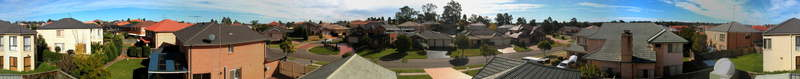
\includegraphics[scale=2.2]{landscape_beaumonthills.jpg}
%\caption{Figure caption}
\end{figure}

This is the only way to get a high resolution panorama and although this
procedure is based on the Microsoft Windows System the basics will apply
to any platform that can run the programs mentioned or similar programs
on the preferred system. If you want a high resolution this is the only
method to use. The first thing needed for a personalised landscape to
superimpose on the horizon display is a 360$\degree$ panorama with a transparent
background. To make this you will need the following:

\begin{itemize}
\item
  A digital camera on a tripod or stable platform
\item
  A program to convert the pictures into a 360$\degree$ panorama
\item
  A program to remove the background and convert the panorama into about
  8 square pictures in PNG format for insertion into Stellarium as the
  sides and if possible a similar square picture of the base you are
  standing on to form the ground. This last requirement is only really
  possible if this area is relatively featureless as the problem of
  knitting a complex base is well nigh impossible.
\item
  Patience. (Maybe a soundproof room so that the swearing wont be heard
  when you press the wrong key and lose an hours work)
\end{itemize}

\subsection{The Camera}\label{the-camera}

Digital cameras are easy and cheaply available these days so whatever
you have should do. One mega-pixel resolution is quite sufficient.

The camera needs to be mounted on a tripod so that reasonably orientated
pictures can be taken. Select a time of day that is quite bright with a
neutral cloudy sky so there will be no shadows and a sky of the same
overall texture. This will make it easier to remove later. The pictures
were all saved in the JPG format which was used as the common format for
all processes up to the removal of the background.

With a camera that takes 4:3 ratio pictures I found 14 evenly spaced
pictures gave the best 360$\degree$ panorama in the program I used to produce
it.

\subsection{Processing into a
Panorama}\label{processing-into-a-panorama}

This is the most complicated part of the process of generating the
panorama. I used two separate programs to do this. Firstly I used The
Gimp to re size the panels to 1024x768 and so make them easier to handle
in the panorama program.

When I had my 14 processed pictures I inserted them into the panorama
program. I first used a program called the Panorama Factory. Version 1.6
is a freebee that works well and can be downloaded from the internet - a
Google search will find it. I later used version 3.4 that is better and
cost about \$40 off the Internet. This program has many options and can
be configured to suit most cameras and can make a seamless 360$\degree$ panorama
in barrel form that will take a highly trained eye to find where the
joins occur.

The resulting panorama was then loaded into The Gimp and trimmed to a
suitable size. Mine ended up 14024 x 1601 pixels. I trimmed the vertical
size to 1024 by cutting back then stretched the 14024 to 14336 pixels,
with almost no distortion, that would allow cutting into 14 1024 x1024
pictures at a later date. If the height of the panorama had been greater
I could have made fewer pictures and so shown more of the foreground.
See figure {[}fig:panorama360{]}.

If you have prominent foreground items like posts wires etc. that occur
in adjacent pictures the panorama program will have difficulty in
discerning them because of the 3D effect and may give double images. I
overcame this by painting out the offending item by cut and paste
between the two pictures. Quite easy with a little practice using the
zoom in facility and I found the MSpaint program the easiest to do this
in.

\begin{figure}[h]
\centering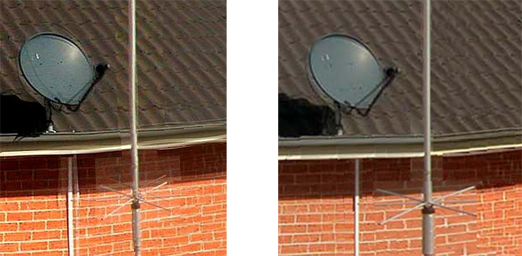
\includegraphics[scale=2.0]{BEAU-3c}
%\caption{Figure caption}
\end{figure}

\subsection{Removing the background to make it
transparent}\label{removing-the-background-to-make-it-transparent}

This is the most complex part of the process and requires a program that
can produce transparency to parts of your picture, commonly called an
alpha channel. Two programs I know of will do this. The very expensive
and sophisticated Adobe Photoshop and a freebee called The Gimp. I used
photoshop to cut the full panorama into 1024 x 1024 textures because it
was the easiest to do accurate cutting but it can be done in TheGimp as
well.

I first used Photoshop to produce the alpha channel because it was the
only way I knew but I now use the GIMP as it is much easier to process
the individual textures than removing the background from the full
panorama.

\begin{enumerate}
\item
  Load the 1st section into TheGimp
\item
  Next create a new empty picture 1024 x 1024 then use the advanced tab
  to make the background color transparency. Copy the original texture
  onto this new picture base so that it exactly fits the frame then
  select layer from the menu and press anchor. This will create a new
  picture with with an alpha channel. By using the select by color and
  lasso etc cut out the parts you don't want this will expose the
  checkerboard background. When you are happy with the removal save the
  texture in *.png format to preserve the alpha layer.
\item
  Do the same with the remaining pictures to make all the components of
  the landscape.
\item
  Make a new directory for the landscape. This should be a sub-directory
  of either the /landscapes or /landscapes directory. The name of the
  directory should be unique to your landscape, and is the landscape ID.
  The convention is to use a single descriptive word in lowercase text,
  for example gueriens. Place your pictures your new directory.
\item
  In your new landscape directory, create a new file called
  landscape.ini file (I used wordpad). Add a line for the
  {[}landscape{]} section. It's probably easiest to copy the
  landscape.ini file for the Gueriens landscape and edit it. Edit the
  name Guereins in every instance to the name you have given your
  landscape. Don't forget to make the number of tex entries agree with
  the number of your pictures. If you haven't made a groundtex picture
  use one of the existing ones from the file or make a square blank
  picture of your own idea. Because I took my pictures from the roof of
  the house I used an edited picture of the roof of my house from Google
  Earth. It was pretty cruddy low resolution but served the purpose.
\item
  Next you need to orientate your picture North with true North. This is
  done roughly by making the arrangement of side1 to siden suit your
  site as close as possible. Now you need to edit the value of
  decor\_angle\_rotatez to move your landscape in azimuth. Edit
  decor\_alt\_angle to move you landscape in altitude to align your
  visible horizon angle. Edit ground\_angle\_rotatez to align your
  ground with the rest of the landscape. Leave the other entries they
  are suitable as is.
\end{enumerate}

After re-starting Stellarium, your landscape will appear in the
landscape folder of the main menu , and can be selected as required.

\section{Making a Spherical Panorama}
\label{making-a-spherical-panorama}

A simpler method of making a panorama is to use the spherical method.
These can be made to create the full panorama using the program
Autostitch. The big advantage of the spherical panorama is that it does
not need a ground panel. However the drawback with the Spherical
panorama is that few computer video cards will reproduce a panorama
larger than 4096 x 2048 pixels and many will not do better than 2048 x
1024 pixels

\begin{figure}[h]
\centering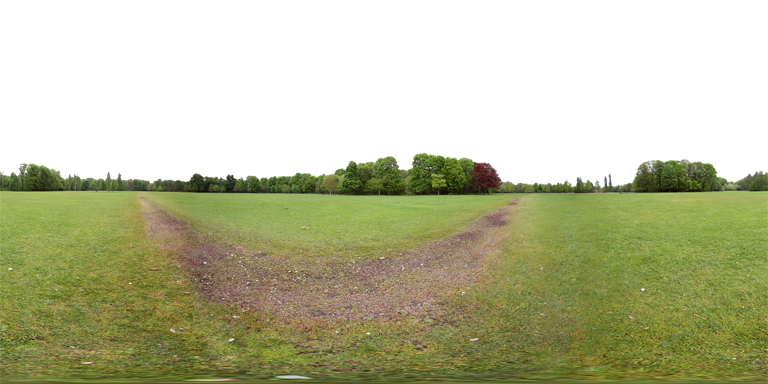
\includegraphics{egarden}
%\caption{Figure caption}
\end{figure}

The Autostitch program is quite easy to use. Make sure your panorama
shots take the ground almost up to your feet and follow the instructions
in the readme file. \href{http://www.example.com}{link title} When the
panorama is finished it will be in *,jpg format. This will need to be
converted to a *.png with transparent background (alpha layer) and have
the sky removed. This can be done in TheGimp as in the multi-panel type.
When the sky is removed make sure you save the landscape in *.png
format.

My computer will only do 2048 by 1024, If I try to load a larger type I
just get a white screen. With this problem I used the following
procedure to make the spherical into a four panel multi-panel landscape
with a very effective ground that matched well

\subsection{Converting a Spherical Panorama into a Multi Panel}
\label{converting-a-spherical-panorama-into-a-multi-panel}

Most computers with standard video cards will not display spherical
panoramas larger than 4096 x 2048 and some will not even go beyond 2048
x 1024. This makes rather poor resolution panaoramas. OK for planets but
not very pretty for your local environment. If the panorama can have a
horizontal section cut out that can keep the detail within a 1024
vertical boundary it is ideal for processing into 1024 x 1024 sections.
When you have the sections proceed as with the previous description

\begin{figure}[h]
\centering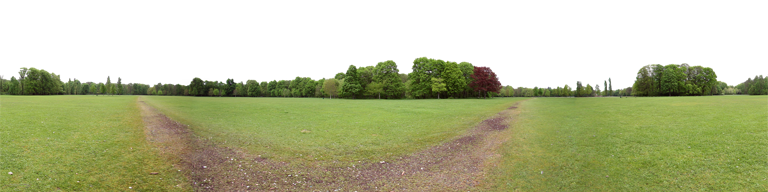
\includegraphics{egarden-narrow}
%\caption{Figure caption}
\end{figure}

I made the egarden into a 4096 x 1024 quite easily because there was a
lot of blank space above the horizon. This would allow 4 panels 1024 x
1024 pixels.in fact if I had a 8192 x 4096 panorama I could have made it
into 8 1024 x 1024 panels. This would have given me quite a high
resolution horizon

\begin{figure}[h]
\centering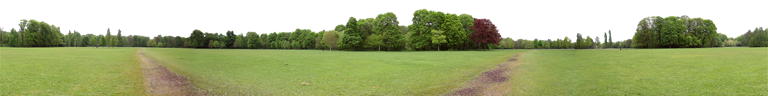
\includegraphics{egarden-narrow-2}
%\caption{Figure caption}
\end{figure}


\begin{enumerate}
\item
  Load the sections into TheGimp and process them into 1024 x 1024
  textures with alpha layers as before.
\item
  Next use a 2048 x 1024 version of the panorama in Stellarium. Drag the
  screen around so it produces a centralised picture on the Stellarium
  screen of the ground at the highest resolution possible and take a
  screen shot. This screen shot can be then processed into a quite
  effective ground texture in TheGimp that can be adjusted to match the
  rest of the panorama.
  \begin{figure}[h]
  \centering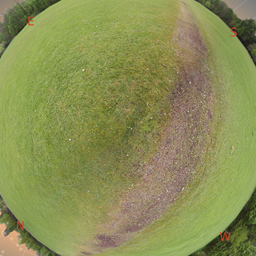
\includegraphics[scale=2.0]{egardembase}
  %\caption{Figure caption}
  \end{figure}
\item
  Make a new directory etc. for the landscape.
\item
  You can make it fit using the variablein the landscape.ini file
  decor\_alt\_angle=xx decor\_angle\_shift=xx and
  decor\_angle\_rotatez=xx.Then the ground can be matched with
  ground\_angle\_shift=xx and ground\_angle\_rotatez=xx.
\item
  Make sure the draw\_ground\_first=1 to ensure that the main panorama
  overplays the ground
\end{enumerate}

After re-starting Stellarium, your landscape will appear in the
landscape tab of the main menu, and can be selected as required.

When the panorama is finished it will be in *.jpg format. It will need
to be converted to a *.png with transparent background (alpha layer) and
have the sky removed. This is done in TheGimp as in the multipanel type.
When the sky is removed make sure you save the landscape in *.png
format.

The drawback with the spherical panorama is that few computer video
cards will reproduce a panorama larger than 4096 x 2048 pixels in
Stellarium and many will not do better than 2048 x 1024 pixels.

My computer will only do 2048 by 1024, If I try to load a larger type I
just get a white screen. With this problem I used the following
procedure to make the spherical into a four panel multi panel landscape
with a very effective ground that matched well.

\section{Making a Fish eye Panorama}
\label{making-a-fish-eye-panorama}

This sort of panorama needs a very expensive fisheye lens on your
camera. It is really only practical for a planetarium display to give a
simple more or less silouette landscape where the ground is completely
obscured. It can only be used with quite small pictures of no more than
1024 x 1024 pixels. Once you have your fisheye texture it must still be
processed in TheGimp to remove the sky and convert into an alpha layer
texture

\begin{figure}[h]
\centering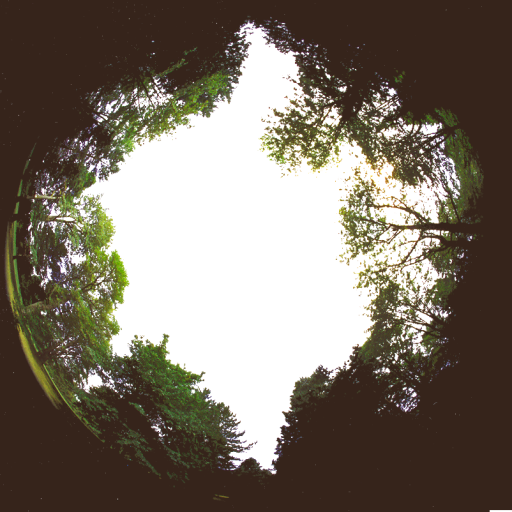
\includegraphics[scale=3.0]{trees_512}
%\caption{Figure caption}
\end{figure}

The sample supplied with Stellarium is called trees. The horizon needs
to be identified and the picture sized so that the panorama above the
horizon is sited to be about 80\% of the total extent and the the
balance of the border filled with a dark colour right up to the horizon.
This will make the horizon in your landscape at 0 degrees.

It is possible to make a synthetic fisheye texture using the same method
as making a ground from a spherical panorama but it is hardly worth the
trouble as even a simple 2048 x 1024 pixel sperical will give a far
better result.

%%% Local Variables: 
%%% mode: latex
%%% TeX-master: "guide"
%%% End: 

%% Part of Stellarium User Guide
%% History: 
%% 2016-04-24 Adapted from GZ's course given at SEAC2015 in Rome.
%% 2016-04-25 Added section on making Nadir image for old_style landscape.
%% State: Current for 0.15.


\chapter{Landscapes}
\label{ch:landscapes}
\chapterauthor*{Georg Zotti}

\newcommand{\landscape}[1]{\textsf{\textit{\footnotesize #1}}}

  
Landscapes are one of the key features that make Stellarium popular.
Originally just used for decoration, since version 10.6 they can be
configured accurately for research and demonstration in ``skyscape
astronomy'', a term which describes the connection of landscape and
the sky above. Configured properly, they can act as reliable proxies
of the real landscapes, so that you can take e.g.\ measurements of
sunrise or stellar alignments, or prepare your next moonrise
photograph, as though you were on-site.

In this chapter you can find relevant information required to
accurately configure Stellarium landscapes, using panoramas created
from photographs taken on-site, optionally supported by horizon
measurements with a theodolite.


Creating an accurate panorama requires some experience with
photography and image processing. However, great open-source tools
have been developed to help you on the job. If you already know other
tools, you should be able to easily transfer the presented concepts to
those other tools.


\section{Stellarium Landscapes}
\label{sec:landscapes:StellariumLandscapes}


As of version 0.15, the available landscape types are:
\begin{description}
\item[polygonal] A point list of measured azimuth/altitude pairs, used
  to define a sharp horizon polygon. The area below the horizon line
  is colored in a single color
  (Section~\ref{sec:landscapes:Polygonal}).
\item[spherical] The simple form to configure a photo-based panorama:
  A single image is used as texture map for the horizon
  (Section~\ref{sec:landscapes:Spherical}).
\item[old\_style] The original photo panorama. This is the most
  difficult to configure, but allows highest resolution by using
  several texture maps (Section~\ref{sec:landscapes:oldStyle}).
\item[fisheye] Another 1-texture approach, utilizing an image made
  with a fisheye lens. This landscape suffers from calibration
  uncertainties and can only be recommended for decoration
  (Section~\ref{sec:landscapes:Fisheye}).
\end{description}

A landscape consists of a \file{landscape.ini} plus the data files
that are referenced from there, like a coordinate list or the
textures. Those reside in a subdirectory of the \file{landscape}
folder inside the Stellarium program directory, or, for own work, in a
subdirectory of the \file{landscape} folder inside your Stellarium
user data directory (see section~\ref{sec:Directories}). 

Let us ssume we want to create a landscape for a place called
Rosenburg.  The location for the files of our new custom landscape
\landscape{Rosenburg} depends on the operating system (see
\ref{sec:Directories}). Create a new subdirectory, and for maximum
compatibility, use small letters and no spaces:

\noindent
\begin{tabular}{ll}
Windows&  \file{C:/Users/YOU/AppData/Roaming/Stellarium/landscapes/rosenburg}\\
Linux&\file{\textasciitilde/.stellarium/landscapes/rosenburg}\\
Mac&\file{\$HOME/Library/Preferences/Stellarium/landscapes/rosenburg}\\
\end{tabular}


% \noindent The user data directory is unfortunately hidden by default
% on all systems. (On UNIX-like systems, directories starting with a
% \file{.} are hidden.) To make it accessible in the Windows file
% explorer, open an Explorer window and select \menu{Organize..., Folder and
% search options}. Make sure folders marked as hidden are still
% displayed. Also, deselect the checkbox to hide known file name
% endings.\footnote{This is a very confusing default setting and in fact
%   a security risk: Consider you receive some file
%   \file{funny.png.exe}. Your explorer displays this as
%   \file{funny.png}. You double-click it, expecting to open some image
%   browser with a funny image. However, you start some unknown program
%   instead, and running this \file{.exe} executable program may turn
%   out to be anything but funny!}
% 

\subsection{Location information}
\label{sec:landscapes:location}

This optional section in \file{landscape.ini} allows automatic loading
of site coordinates if this option is activated in the program
GUI (see~\ref{sec:gui:view:landscape}). For our purposes we should consider especially the coordinates in
the location section mandatory!

\begin{configfile}
[location]
planet = Earth
country = Austria
name = KGA Rosenburg
latitude = +48d38'3.3"
longitude = +15d38'2.8"
altitude = 266
light_pollution = 1
atmospheric_extinction_coefficient = 0.2
display_fog = 0
atmospheric_temperature = 10.0
atmospheric_pressure = 1013.0
\end{configfile}
%
Where:
\begin{description}
\item[\var{planet}] Is the English name of the solar system body for
  the landscape.
\item[\var{latitude}] Is the latitude of site of the landscape in
  degrees, minutes and seconds. Positive values represent North of the
  equator, negative values South of the equator.
\item[\var{longitude}] Is the longitude of site of the
  landscape. Positive values represent East of the Greenwich Meridian
  on Earth (or equivalent on other bodies), Negative values represent
  Western longitude.
\item[\var{altitude}] Is the altitude of the site of the landscape in meters.
\item[\var{country}] (optional) Name of the country the location is in.
\item[\var{state}] (optional) Name of the state the location is in.
\item[\var{name}] (optional) Name of the location. This may contain
  spaces, but keep it short to have it fully visible in the
  selection box.
\end{description}
%
Since V0.11, there are a few more optional parameters that can be
loaded if the according switch is active in the landscape selection
panel. If they are missing, the parameters do not change to defaults.

\begin{description}
\item[\var{light\_pollution}] (optional) Light pollution of the site,
  given on the Bortle Scale (1: none \ldots 9: metropolitan; see
  Appendix \ref{ch:BortleScale}). If negative or absent, no change
  will be made.
\item[\var{atmospheric\_extinction\_coefficient}] (optional, no change
  if absent.) Extinction coefficient (mag/airmass) for this site.
\item[\var{atmospheric\_temperature}] (optional, no change if absent.)
  Surface air temperature (Degrees Celsius). Used for refraction. Set
  to -1000 to explicitly declare "no change".
\item[\var{atmospheric\_pressure}] (optional, no change if absent.)
  Surface air pressure (mbar; would be 1013 for "normal" sea-level
  conditions). Used for refraction. Set to -2 to declare "no change",
  or -1 to compute from altitude.
\item[\var{display\_fog}] (optional, -1/0/1, default=-1) You may want
  to preconfigure setting 0 for a landscape on the Moon. Set -1 to
  declare "no change".
\end{description}


\subsection{Polygonal landscape}
\label{sec:landscapes:Polygonal}

This landscape type has been added only recently (since 0.13) to allow
the use of measured horizons. Users of \program{Cartes du
  Ciel}\footnote{SkyChart / Cartes du Ciel planetarium:
  \url{http://www.ap-i.net/skychart/en/start}} will be happy to hear
that the format of the list of measurements is compatible.

This is the technically simplest of the landscapes, but may be used to
describe accurately measured horizon lines. The file that encodes
horizon altitudes can also be used in all other landscape types. If
present there, it will be used to define object visibility (instead of
the opacity of the landscape photo textures) and, if
\var{horizon\_line\_color} is defined, will be plotted.

There is a small caveat: Sometimes, there may appear vertical lines
from some corners towards the zenith or the mathematical horizon,
e.g.\ if there is a vertex including azimuth 0 or 180. If this
irritates you, just offset this azimuth minimally (e.g., 180.00001).

The \file{landscape.ini} file for a polygonal type landscape looks
like this (this example is based on the \landscape{Geneve} landscape
which was borrowed from Cartes du Ciel and comes with Stellarium):

\begin{configfile}
[landscape]
name = Geneve
type = polygonal
author = Georg Zotti; Horizon definition by Patrick Chevalley
description = Horizon line of Geneve. 
              Demonstrates compatibility with 
              horizon descriptions from Cartes du Ciel.
polygonal_horizon_list = horizon_Geneve.txt
polygonal_angle_rotatez = 0
ground_color = .15,.45,.45
horizon_line_color = .75,.45,.45
\end{configfile}
%
Where:
\begin{description}
\item[\var{name}] appears in the landscape tab of the configuration window.
\item[\var{type}] identifies the method used for this landscape. \var{polygonal} in this case.
\item[\var{author}] lists the author(s) responsible for images and composition.
\item[\var{description}] gives a short description visible in the
  selection panel. The text can be superseded by optional
  \file{description.<lang>.utf8} files.
\item[\var{polygonal\_horizon\_list}] is the name of the horizon data file for this landscape.
\item[\var{polygonal\_horizon\_list\_mode}] (optional) the two first
  columns in the list are numbers: azimuth and altitude or zenith
  distance, in either degrees or radians or gradians(gon). The value
  must be one of \var{azDeg\_altDeg}, \var{azDeg\_zdDeg}, \var{azRad\_altRad},
    \var{azRad\_zdRad}, \var{azGrad\_altGrad}, \var{azGrad\_zdGrad}. Default:
  \var{azDeg\_altDeg}
\item[\var{polygonal\_angle\_rotatez}] (optional, default=0) Angle
  (degrees) to adjust azimuth. This may be used to apply a (usually)
  small offset rotation, e.g. when you have measured the horizon in a
  grid-based coordinate system like UTM and have to compensate for the
  meridian convergence.
\item[\var{ground\_color}] (optional, default=\var{0,0,0}, i.e.,
  black) Color for the area below the horizon line. Each R,G,B
  component is a float within 0..1.
\item[\var{horizon\_line\_color}] (optional, default: invisible) used
  to draw a polygonal horizon line. Each R,G,B component is a float
  within 0..1.
\item[\var{minimal\_brightness}] (optional) Some minimum brightness to
  keep landscape visible. Default=-1, i.e., use
  \var{minimal\_brightness} from the \var{[landscape]} section in the
  global \file{config.ini}.
\item[\var{minimal\_altitude}] (optional, default=-2) Some sky
  elements, e.g.\ stars, are not drawn below this altitude to increase
  performance. Under certain circumstances you may want to specify
  something else here. (since V0.14)
\end{description}


\subsection{Spherical landscape}
\label{sec:landscapes:Spherical}

This method uses a more usual type of panorama -- the kind which is
produced directly from software such as \program{autostitch} or
\program{Hugin}\footnote{\url{http://hugin.sourceforge.net/}}.  The
\landscape{Moon} landscape which comes with Stellarium provides a
minimal example of a \file{landscape.ini} file for a spherical type
landscape:

\begin{configfile}
[landscape]
name = Moon
type = spherical
maptex = apollo17.png
\end{configfile}
A more elaborate example is found with the \landscape{Grossmugl} landscape: 

\begin{configfile}
[landscape]
name = Grossmugl
type = spherical
author = Guenther Wuchterl, Kuffner-Sternwarte.at; 
         Lightscape: Georg Zotti
description = Field near Leeberg, Grossmugl (Riesentumulus), 
              Austria - Primary Observing Spot of the Grossmugl 
              Starlight Oasis - http://starlightoasis.org
maptex = grossmugl_leeberg_crop11.25.png
maptex_top=11.25 
maptex_fog = grossmugl_leeberg_fog_crop22.5.png
maptex_fog_top = 22.5
maptex_fog_bottom = -22.5
maptex_illum = grossmugl_leeberg_illum_crop0.png
maptex_illum_bottom = 0
angle_rotatez=-89.1
minimal_brightness = 0.0075
polygonal_horizon_list = horizon_grossmugl.txt
polygonal_angle_rotatez=0
horizon_line_color =  .75,.45,.45
minimal_altitude = -1
\end{configfile}
Where:
\begin{description}
\item[\var{name}] appears in the landscape tab of the configuration window. This name may be translated.
\item[\var{type}] identifies the method used for this
  landscape. \var{spherical} in this case.
\item[\var{author}] lists the author(s) responsible for images and
  composition.
\item[\var{description}] gives a short description visible in the
  selection panel. The text will be superseded by optional
  \file{description.<lang>.utf8} files.
\item[\var{maptex}] is the name of the image file for this landscape.
\item[\var{maptex\_top}] (optional; default=90) is the altitude angle
  of the top edge.
\item[\var{maptex\_bottom}] (optional; default=-90) is the altitude
  angle of the bottom edge. Usually you will not require this, or else
  there will be a hole at your feet. ;-)
\item[\var{maptex\_fog}] (optional; default: no fog) is the name of
  the fog image file for this landscape.
\item[\var{maptex\_fog\_top}] (optional; default=90) is the altitude
  angle of the top edge of the fog texture. Useful to crop away parts
  of the image to conserve texture memory.
\item[\var{maptex\_fog\_bottom}] (optional; default=-90) is the
  altitude angle of the bottom edge.
\item[\var{maptex\_illum}] (optional; default: no illumination layer)
  is the name of the nocturnal illumination/light pollution image file
  for this landscape.
\item[\var{maptex\_illum\_top}] (optional; default=90) is the altitude
  angle of the top edge, if you have light pollution only close to the
  horizon.
\item[\var{maptex\_illum\_bottom}] (optional; default=-90) is the
  altitude angle of the bottom edge.
\item[\var{angle\_rotatez}] (optional, default=0) Angle (degrees) to
  adjust azimuth. If 0, the left/right edge is due east.
\item[\var{tesselate\_rows}] (optional, default=20) This is the number
  of rows for the maptex. If straight vertical edges in your landscape
  appear broken, try increasing this value, but higher values require
  more computing power. Fog and illumination textures will have a
  similar vertical resolution.
\item[\var{tesselate\_cols}] (optional, default=40) If straight
  horizontal edges in your landscape appear broken, try increasing.
\item[\var{polygonal\_horizon\_list}] (optional) is the name of the
  (measured) horizon data file for this landscape. Can be used to
  define the exact position of the horizon. If missing, the texture
  can be queried for horizon transparency (for accurate object
  rising/setting times)
\item[\var{polygonal\_horizon\_list\_mode}] (optional) see \ref{sec:landscapes:Polygonal}  % 
      % the two first columns in the list are numbers: azimuth and altitude or zenith distance, in either degrees or radians or gradians(gon). 
      % The value must be one of azDeg_altDeg|azDeg_zdDeg|azRad_altRad|azRad_zdRad|azGrad_altGrad|azGrad_zdGrad. Default: azDeg_altDeg
\item[\var{polygonal\_angle\_rotatez}] (optional, default=0) see \ref{sec:landscapes:Polygonal}  %Angle (degrees) to adjust azimuth. This may be used to apply a (usually) small offset rotation, e.g. when you have measured the horizon in a grid-based coordinate system like UTM and have to compensate for the meridian convergence.
\item[\var{horizon\_line\_color}] see \ref{sec:landscapes:Polygonal}  %(optional, default: invisible) used to draw a polygonal horizon line.
\item[\var{minimal\_brightness}]  see \ref{sec:landscapes:Polygonal}  %(optional, default=-1, i.e. use preset landscape/minimal_brightness from global config.ini) Some minimum brightness to keep landscape visible.
\item[\var{minimal\_altitude}] (optional, default=-2) Some sky
  elements, e.g.\ stars, are not drawn below this altitude for
  efficiency. Under certain circumstances (e.g.\ for space station
  panoramas where you may have sky below your feet, or for deep
  valleys/high mountains, you may want to specify something else
  here. (since V0.14)
\end{description}
%
To save texture memory, %since V0.13 
you can trim away the transparent
sky and define the angle \var{maptex\_top}. Likewise,
\var{fogtex\_top}, \var{fogtex\_bottom}, \var{maptex\_illum\_top} and
\var{maptex\_illum\_top}. You should then stretch the texture to a
full power of 2, like $4096\times1024$ (but note that some hardware is
even limited to 2048 pixels). The easiest method to create perfectly
aligned fog and illumination layers is with an image editor that
supports layers like the \program{GIMP} or \program{Photoshop}. Fog
and Light images should have black background.


\subsection{High resolution (``Old Style'')  landscape}
\label{sec:landscapes:oldStyle}

The \var{old\_style} or multiple image method works by having the
360\degree panorama of the horizon (without wasting too much texture
memory with the sky) split into a number of reasonably small
\emph{side textures}, and a separate \emph{ground texture}. This has
the advantage over the single-image method that the detail level of
the horizon can be increased without ending up with a single very
large image file, so this is usable for either very high-resolution
panoramas or for older hardware with limited capabilities. The ground
texture can be a different resolution than the side textures. Memory
usage may be more efficient because there are no unused texture parts
like the corners of the texture file in the fish-eye method. It is
even possible to repeat the horizon several times (for purely
decorative purpose). The side textures are mapped onto curved
(spherical ring or cylinder) walls
(Fig.~\ref{fig:landscapes:oldStyle}).

\begin{figure}[tb]
  \centering
   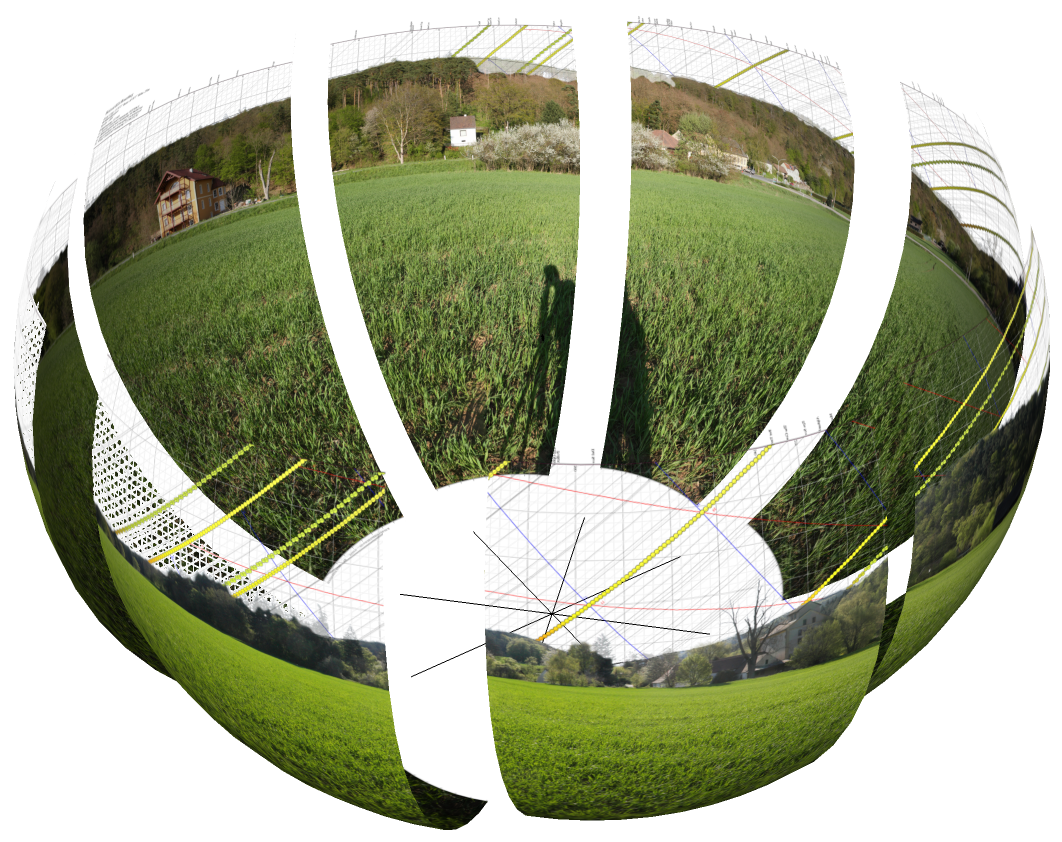
\includegraphics[width=10cm]{Rosenburg-Demo.png}
   \caption{Old\_style landscape: eight parts delivering a
     high-resolution panorama. The bottom (ground) texture, drawn on a flat
     plane, is not shown here.}
  \label{fig:landscapes:oldStyle}
\end{figure}

On the negative side, it is more difficult to create this type of
landscape -- merging the ground texture with the side textures can
prove tricky. (\program{Hugin} can be used to create also this file,
though. And on the other hand, you can replace this by something else
like a site map.) The contents of the \file{landscape.ini} file for
this landscape type is also somewhat more complicated than for other
landscape types. Here is the \file{landscape.ini} file which describes
our \landscape{Rosenburg} landscape\footnote{the \var{groundtex}
  \file{grassground.png} mentioned here has been taken from the
  \landscape{Guereins} landscape.}:

\begin{configfile}
[landscape]
name = KGA Rosenburg
author = Georg Zotti, VIAS/ASTROSIM
description = KGA Rosenburg
type = old_style
nbsidetex = 8
tex0 = Horiz-0.png
tex1 = Horiz-1.png
tex2 = Horiz-2.png
tex3 = Horiz-3.png
tex4 = Horiz-4.png
tex5 = Horiz-5.png
tex6 = Horiz-6.png
tex7 = Horiz-7.png
nbside = 8
side0 = tex0:0:0:1:1
side1 = tex1:0:0:1:1
side2 = tex2:0:0:1:1
side3 = tex3:0:0:1:1
side4 = tex4:0:0:1:1
side5 = tex5:0:0:1:1
side6 = tex6:0:0:1:1
side7 = tex7:0:0:1:1
groundtex = grassground.png
ground = groundtex:0:0:1:1
nb_decor_repeat = 1
decor_alt_angle =  82
decor_angle_shift = -62
; Rotatez deviates from -90 by the Meridian Convergence. 
; The original landscape pano is grid-aligned, not north-aligned!
decor_angle_rotatez =  -90.525837223
ground_angle_shift = -62
ground_angle_rotatez =  44.474162777
draw_ground_first = 1
fogtex = fog.png
fog_alt_angle = 20
fog_angle_shift = -3
fog = fogtex:0:0:1:1
calibrated = true
[location]
planet = Earth
latitude = +48d38'3.3"
longitude = +15d38'2.8"
altitude = 266
light_pollution = 1
atmospheric_extinction_coefficient = 0.2
display_fog = 0
atmospheric_temperature = 10.0
atmospheric_pressure = 1013.0
\end{configfile}
%
Where:
\begin{description}
\item[\var{name}] is the name that will appear in the landscape tab of the configuration window for this landscape
\item[\var{type}] should be \var{old\_style} for the multiple image method.
\item[\var{author}] lists the author(s) responsible for images and composition.
\item[\var{description}] gives a short description visible in the
  selection panel. The text will be superseded by optional
  \file{description.<lang>.utf8} files.
\item[\var{nbsidetex}] is the number of side textures for the landscape.
\item[\var{tex0 ... tex<nbsidetex-1>}] are the side texture file
  names. These should exist in the \file{textures / landscapes /
    landscape} directory in PNG format.
\item[\var{light0 ... light<nbsidetex-1>}] are optional textures. If
  they exist, they are used as overlays on top of the respective
  \var{tex<...>} files and represent nocturnal illumination,
  e.g. street lamps, lit windows, red dots on towers, sky glow by city
  light pollution, \ldots Empty (black) panels can be omitted. They
  are rendered exactly over the \var{tex<...>} files even when the PNG
  files have different size. If you need your light pollution higher in
  the sky, you must use a spherical or fisheye
  landscape.% (New feature, V0.13.1)
\item[\var{nbside}] is the number of side textures
\item[\var{side0 \ldots side<nbside-1>}] are the descriptions of how
  the side textures should be arranged in the program. Each
  description contains five fields separated by colon characters
  (\var{:}). The first field is the ID of the texture
  (e.g. \var{tex0}), the remaining fields are the texture coordinates
  (\var{x0:y0:x1:y1}) used to place the texture in the scene. If you
  want to use all of the image, this will just be \var{0:0:1:1}.
\item[\var{groundtex}] is the name of the ground texture file. (This
  could also be a diagram e.g. indicating the mountain peaks!)
%\item[\var{ground}] [NO LONGER USED] used to be the description of the projection of the ground texture in the scene.
\item[\var{fogtex}] is the name of the texture file for fog in this
  landscape. Fog is mapped onto a simple cylinder.\footnote{In very wide-angle
  views, the fog cylinder may become visible in the corners.} Note that for this
  landscape, accurate overlay of fog and landscape is only guaranteed if
  \var{calibrated=true} and \var{tan\_mode=true}. 
%\item[\var{fog}] [NO LONGER USED] used to be the description of the projection of the fog texture in the scene.
\item[\var{nb\_decor\_repeat}] is the number of times to repeat the
  side textures in the 360 panorama. (Useful photo panoramas should
  have \var{1} here)
\item[\var{decor\_alt\_angle}] (degrees) is the vertical angular
  extent of the textures (i.e. how many degrees of the full altitude
  range they span).
\item[\var{decor\_angle\_shift}] (degrees) vertical angular offset of
  the scenery textures, at which height the bottom line of the side
  textures is placed.
\item[\var{decor\_angle\_rotatez}] (degrees) angular rotation of the
  panorama around the vertical axis. This is handy for rotating the
  landscape so North is in the correct direction. Note that for
  historical reasons, a landscape with this value set to zero degrees
  has its leftmost edge pointing towards east.
\item[\var{ground\_angle\_shift}] (degrees) vertical angular offset of
  the ground texture, at which height the ground texture is placed.
\item[\var{ground\_angle\_rotatez}] (degrees) angular rotation of the
  ground texture around the vertical axis. When the sides are rotated,
  the ground texture may need to be rotated as well to match up with
  the sides.
\item[\var{fog\_alt\_angle}] (degrees) vertical angular size of the
  fog cylinder - how fog looks. Accurate vertical size requires
  \var{calibrated=true}.
\item[\var{fog\_angle\_shift}] (degrees) vertical angular offset of
  the fog texture - at what height is it drawn. Accurate vertical
  placement requires \var{calibrated=true}.
\item[\var{draw\_ground\_first}] if 1 the ground is drawn in front of
  the scenery, i.e. the side textures will overlap over the ground
  texture.
\item[\var{calibrated}] (optional). New since V0.10.6: Only if true,
  \var{decor\_alt\_angle} etc. really work as documented above. The
  (buggy) old code was left to work with the landscapes already
  existing. Note that with ``uncalibrated'' landscapes, sunrise
  computations and similar functionality which requires an accurate
  horizon line will not work.
\item[\var{tan\_mode}] (optional, not used in this file). If true, the
  panorama image must be in in cylindrical, not equirectangular
  projection. Finding \var{decor\_alt\_angle} and
  \var{decor\_angle\_shift} may be a bit more difficult with this, but
  now (V0.13) works also with calibrated. A fog image created as
  overlay on the pano will be perfectly placed.
\item[\var{decor\_angle\_rotatez}] angular rotation of the scenery
  around the vertical axis. This is handy for rotating the landscape
  so North is in the correct direction. If 0, the left edge of
  \var{tex0} is due east.
\item[\var{ground\_angle\_shift}] vertical angular offset of the
  ground texture, at which height the ground texture is placed. Values
  above -10 are not recommended for non-photographic content (e.g., a
  map) due to high distortion.
\item[\var{ground\_angle\_rotatez}] angular rotation of the ground
  texture around the vertical axis. When the sides are rotated, the
  ground texture may need to be rotated as well to match up with the
  sides. If 0, east is up. if North is up in your image, set this to
  90. Note that adjustments of \var{decor\_angle\_rotatez} require
  adjustments of this angle in the opposite direction!
\item[\var{fog\_alt\_angle}] vertical angular size of the fog cylinder.
\item[\var{fog\_angle\_shift}] vertical angular offset of the fog cylinder.
\item[\var{draw\_ground\_first}] if 1, the ground is drawn before the
  sides, i.e.\ the side textures may overlap the ground texture if
  \var{ground\_angle\_shift} > \var{decor\_angle\_shift}.
\item[\var{polygonal\_horizon\_list}] (optional) see \ref{sec:landscapes:Polygonal} %is the name of the (measured) horizon data file for this landscape. Can be used to query horizon transparency (for accurate object rising/setting times)
\item[\var{polygonal\_horizon\_list\_mode}] (optional) see \ref{sec:landscapes:Polygonal}  %the two first columns in the list are numbers: azimuth and altitude or zenith distance, in either degrees or radians or gradians(gon). The value must be one of azDeg_altDeg|azDeg_zdDeg|azRad_altRad|azRad_zdRad|azGrad_altGrad|azGrad_zdGrad. Default: azDeg_altDeg
\item[\var{polygonal\_angle\_rotatez}] (optional, default=0) see \ref{sec:landscapes:Polygonal} %Angle (degrees) to adjust azimuth. This may be used to apply a (usually) small offset rotation, e.g. when you have measured the horizon in a grid-based coordinate system like UTM and have to compensate for the meridian convergence.
\item[\var{horizon\_line\_color}] see \ref{sec:landscapes:Polygonal}  % (optional, default: invisible) used to draw a polygonal horizon line.
\item[\var{minimal\_brightness}]  see \ref{sec:landscapes:Polygonal} % (optional, default=-1, i.e. use landscape/minimal\_brightness from global config.ini) Some minimum brightness to keep landscape visible.
\item[\var{minimal\_altitude}] see \ref{sec:landscapes:Polygonal}  % (optional, default=-2) Some sky elements, e.g. stars, are not drawn below this altitude. Under certain circumstances you may want to specify something else here. (since V0.14) 
\end{description}


\subsection{Fisheye landscape}
\label{sec:landscapes:Fisheye}

The \landscape{Trees} landscape that is provided with Stellarium is an
example of the single fish-eye method, and provides a good
illustration. The centre of the image is the spot directly above the
observer (the zenith). The point below the observer (the nadir)
becomes a circle that just touches the edges of the image. The
remaining areas of the image (the corners outside the circle) are not
used.

\begin{figure}[t]
\centering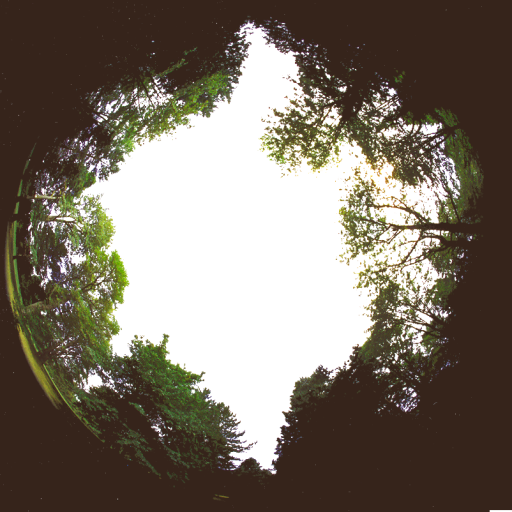
\includegraphics[scale=3.0]{trees_512}
\caption{Texture for the \landscape{Trees} Fisheye landscape.}
\label{fig:landscapes:Fisheye}
\end{figure}


The image file (Fig.~\ref{fig:landscapes:Fisheye}) should be saved in
PNG format with alpha transparency. Whereever the image is transparent
Stellarium will render the sky.

The \file{landscape.ini} file for a fish-eye type landscape looks like
this (this example is based on the \landscape{Trees} landscape which
comes with Stellarium):

\begin{configfile}
[landscape]
name = Trees
type = fisheye
author = Robert Spearman. Light pollution image: Georg Zotti
description = Trees in Greenlake Park, Seattle
maptex = trees_512.png
maptex_illum = trees_illum_512.png
maptex_fog = trees_fog_512.png
texturefov = 210
angle_rotatez = 17
tesselate_rows = 28
tesselate_cols = 60
\end{configfile}
Where:
\begin{description}
\item[\var{name}] appears in the landscape tab of the configuration window.
\item[\var{type}] identifies the method used for this landscape. \var{fisheye} in this case.
\item[\var{author}] lists the author(s) responsible for images and composition.
\item[\var{description}] gives a short description visible in the
  selection panel. The text will be superseded by optional
  \file{description.<lang>.utf8} files.
\item[\var{maptex}] is the name of the image file for this landscape.
\item[\var{maptex\_fog}] (optional) is the name of the fog image file for this landscape.
\item[\var{maptex\_illum}] (optional) is the name of the nocturnal
  illumination/light pollution image file for this landscape.
\item[\var{texturefov}] is the field of view that the image covers in degrees.
\item[\var{angle\_rotatez}] (optional) Angle (degrees) to adjust azimuth.
\item[\var{tesselate\_rows}] (optional, default=20) If straight edges
  in your landscape appear broken, try increasing.
\item[\var{tesselate\_cols}] (optional, default=40) If straight edges
  in your landscape appear broken, try increasing.
\item[\var{polygonal\_horizon\_list}] (optional) see \ref{sec:landscapes:Polygonal}  %is the name of the (measured) horizon data file for this landscape.
\item[\var{polygonal\_horizon\_list\_mode}] (optional) see \ref{sec:landscapes:Polygonal} 
%
%  the two first columns in the list are numbers: azimuth and altitude or zenith distance, in either degrees or radians or
%  gradians(gon). The value must be one of \var{azDeg\_altDeg | azDeg\_zdDeg | azRad\_altRad | azRad\_zdRad | azGrad\_altGrad |  azGrad\_zdGrad}. Default: \var{azDeg\_altDeg}
%
\item[\var{polygonal\_angle\_rotatez}] (optional, default=0) see \ref{sec:landscapes:Polygonal} % Angle (degrees) to adjust azimuth. This may be used to apply a (usually) small offset rotation, e.g.\ when you have measured the horizon in a grid-based coordinate system like UTM and have to compensate for the meridian convergence.
\item[\var{horizon\_line\_color}] see \ref{sec:landscapes:Polygonal} % (optional, default: invisible) used to draw a polygonal horizon line.
\item[\var{minimal\_brightness}]  see \ref{sec:landscapes:Polygonal} % (optional, default=-1, i.e. use preset \var{landscape/minimal\_brightness} from global \file{config.ini}) Some minimum brightness to keep landscape visible.
\item[\var{minimal\_altitude}] see \ref{sec:landscapes:Polygonal} % (optional, default=-2) Some sky elements, e.g. stars, are not drawn below this altitude. Under certain circumstances you may want to specify something else here. (since V0.14) 
\end{description}


\subsection{Description}
\label{sec:landscapes:Description}

The short \var{description} entry in \file{landscape.ini} will be
replaced by the contents of an optional file
\file{description.<LANG>.utf8}. \file{<LANG>} is the ISO~639-1
language code, or its extension which contains language and country
code, like \file{pt\_BR} for Brazilian Portuguese. The long
description requires the file \file{description.en.utf8}, this is
\texttt{en=english} text with optional HTML tags for sections, tables,
etc. You can also have embedded images in the HTML (Views of sacred
landscapes, other informative images, \ldots?), just make them PNG
format please. The length of the description texts is not limited, you
have room for a good description, links to external resources,
whatever seems suitable.

If you can provide other languages supported by Stellarium, you can
provide translations yourself, else Stellarium translators \emph{may}
translate the English version for you. (It may take years though.) The file
ending \file{.utf8} indicates that for special characters like ÄÖÜßáé
you should use UTF8 encoding. If you write only English/ASCII, this may not
be relevant.



\subsection{Gazetteer}
\label{sec:landscapes:Gazetteer}

\newFeature{0.14}
An optional feature for landscapes is a gazetteer function, i.e., labels for
landscape features. The \landscape{Grossmugl} landscape demonstrates
an example and should be self-explanatory. This is again multilingual,
so the files are called \file{gazetteer.<LANG>.utf8}.

\begin{configfile}[\scriptsize]
# demo gazetteer for Grossmugl landscape.
# Can be used to better describe the landscape, 
# i.e. show labels on landscape features.
# Fields must be separated by vertical line, 
# label must not have such a vertical line.
# Comments have this hash mark in first column. 
# coordinates in degrees from true North. 
# line towards zenith draws a single line strictly upward.
# label is centered on line endpoint. 
# Azimuth | Altitude | degrees        | azimuth | label
#         |          | towards zenith |  shift  |               
113.66    | 5.5      |     4          |   -6    | Leeberg
35        | 1.5      |     2.5        |    0    | Grossmugl
335       | 2        |     2          |    0    | Steinabrunn
305       | 2        |     1          |    0    | Ringendorf
180       | 2        |     2          |    0    | Vienna (30km)
135       | 2        |     0.5        |    0    | Wind power plant Strasshof
\end{configfile}


\newpage

\section{Creating Panorama Photographs for Stellarium}
\label{sec:landscapes:PanoramaPhotography}

\subsection{Panorama Photography}
\label{sec:landscapes:PanoramaPhotography:Photography}

Traditional film-based panorama photography required dedicated cameras with curved
film holders and specialized lenses
(Figure~\ref{fig:landscapes:panoCam}).


\begin{figure}[tbp]
  \centering
 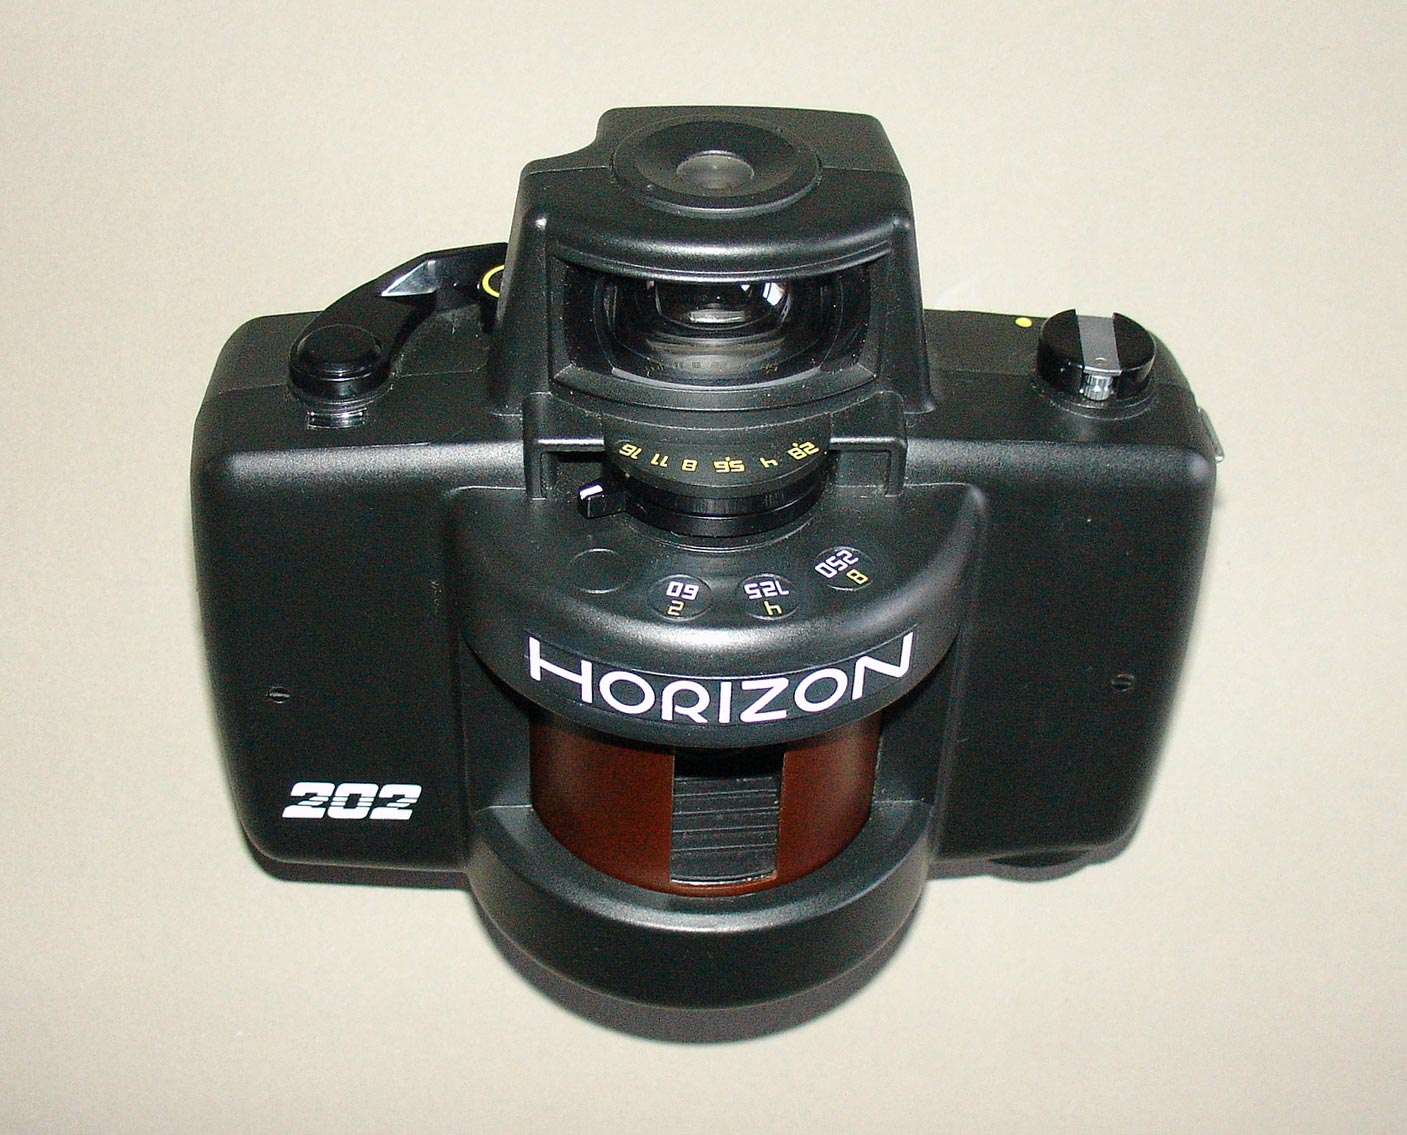
\includegraphics[width=9cm]{Horizon202.jpg}
 \caption{Zenit ``Horizon 202'' panorama camera with rotating lens for
   35mm film. \footnotesize{(Source: Wikipedia, ``Horizon202'' by
     BillC - Own Work. Licensed under CC BY-SA 3.0 via Wikimedia
     Commons -
     \url{https://commons.wikimedia.org/wiki/File:Horizon202.jpg\#mediaviewer/File:Horizon202.jpg})}}
  \label{fig:landscapes:panoCam}
\end{figure}



\begin{figure}[tbp]
  \centering
  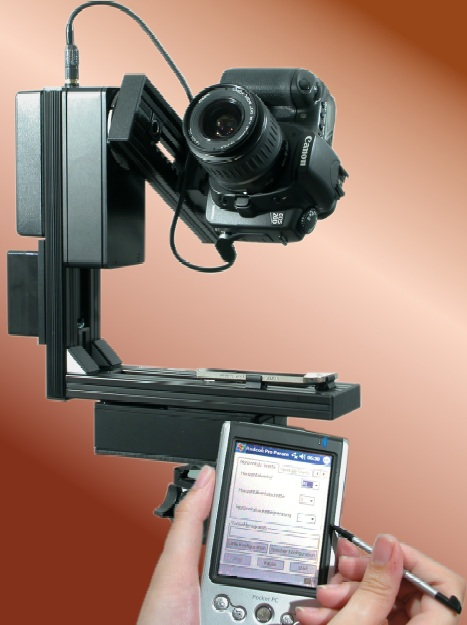
\includegraphics[width=7cm]{Rodeon_vr_head_01.jpg}
  \caption{Automated panorama head. \footnotesize{(Source: Wikipedia \url{https://de.wikipedia.org/wiki/Panoramakamera\#mediaviewer/File:Rodeon_vr_head_01.jpg})}}
  \label{fig:landscapes:panoHead}
\end{figure}


Digital photography has brought a revolution also in this field, and it has
become quite easy to create panoramas simply by taking a series of
photographs with a regular camera on the same spot and combining them
with dedicated software.

A complete panorama photo visually encloses the observer like the
mental image that astronomers have been using for millennia: the
celestial sphere. If we want to document the view, say, in a big hall
like a church, optimal results will be gained with a camera on a
tripod with a specialized panorama head (Figure~\ref{fig:landscapes:panoHead}) which assures the camera
rotates around the \emph{entrance pupil}\footnote{In many references
  you will find ``Nodal Point'' mentioned here. But see these:
  \url{http://en.wikipedia.org/wiki/Cardinal_point_\%28optics\%29\#Nodal_points},
  \url{http://web.archive.org/web/20060513074042/http://doug.kerr.home.att.net/pumpkin/Pivot_Point.pdf},
  \url{http://www.janrik.net/PanoPostings/NoParallaxPoint/TheoryOfTheNoParallaxPoint.pdf}
} of the lens in order to avoid errors by the parallax shift observed
on photographs taken on adjacent but separate positions.


Often however, both the upper half of the observer's environment (the
sky) and the ground the photographer is standing on, are regarded of
lesser importance, and only a series of laterally adjacent photographs
is taken and combined into a cylindrical or spherical ring that shows 
the landscape horizon, i.e.,  where ground and sky meet. If the
closest object of interest is farther away that a few metres,
requirements on parallax avoidance are far less critical, and the author
has taken lots of landscape panoramas with a camera on the usual
tripod screw, and even more entirely without a tripod. However, any visible errors
that are caused by a shifted camera will require more effort in
postprocessing.

When you have no tripod, note that \emph{you must not rotate the
  camera on your outstretched arm!} Rather, the camera's entrance
pupil must be rotated, so you should appear to dance around the
camera!

The images should match in brightness and white balance. If you can
shoot in RAW, do so to be able to change white balance later. If the
camera can only create JPG, ensure you have set the camera to a suitable white balance
before taking the photos and not to ``auto'', because this may find different settings and
thus give colour mismatches. Exposure brightness differences can be
largely removed during stitching, but good, well-exposed original
shots always give better results.

As a general recommendation, the images of a panorama should be taken
from left to right, else please accordingly invert some of the
instructions given below.

There are several panorama making programs. Often they are included in
the software that comes with a digital camera and allow the creation
of simple panoramas. Other software titles are available for
purchase. However, there is one cost-free open-source program
that does everything we need for our task, and much more:


\subsection{Hugin Panorama Software}
\label{sec:landscapes:Hugin}

\program{Hugin}\footnote{\url{http://hugin.sourceforge.net/}}, named
after one of the ravens that sits on Odin's shoulder and tells him
about the world, is a user-friendly catch-all package with graphical
user interface that allows creating panoramas with a single
application. Actually, \program{Hugin} is a GUI application which
calls several specialized sub-programs with fitting parameters.  The
instructions are based on \program{Hugin V2014.0} and
\program{2015.0}.

Typically digital images come in JPG format with information about
camera, lens, and settings stored in invisible metadata in the EXIF
format. When \program{Hugin} reads such images, it can automatically derive
focal length, field of view, and exposure differences (exposure time,
aperture, color balance) to create panoramas as easily as
possible. 

After starting \program{Hugin} for the first time, select \menu{Interface > Expert} to release several
options not visible to ``beginners''.  In the Preferences dialog
(\menu{Files > Preferences}), edit number of CPU to match the number of
cores in your computer and allow parallel processing. E.g., if you
have an Intel Core-i7, you usually can set up to 8 cores (4 cores with
hyperthreading; but maybe leave one core for your other tasks while
you wait for a processing job?).  If your PC is equipped with a
modern programmable graphics card, you can enable its use in the \menu{Programs} tab
with activating ``Use GPU for remapping''.

After that, we are ready for creating our panoramas.


\subsection{Regular creation of panoramas}
\label{sec:landscapes:Hugin:regular}

The graphical user interface (GUI) consists of a main menu, symbols, and 4 tabs. We start on the tab Photos. 
\begin{itemize}
\item \button{Add images\ldots} Opens a file browser. Select the images which you
  want to stitch. Usually, lens data (focal length, field of view,
  \ldots) are read from the EXIF data. If those are not available
  (e.g. cheap cameras, images scanned from film), you can enter those
  data on loading or later.  The images are now listed in the file
  list, and you can edit image parameters by marking one or more, and
  then choosing from the context menu which you get from pressing the
  right mouse button. In case you have used different lenses (or
  inadvertently used different focal lengths of a zoom lens), you can
  assign separate lenses to the images.

  Caveat: If you have resized the images, or produced copied on your
  RAW converter with non-native resolution, the Field of View (FoV) in
  \program{Hugin} may be misidentified. You must edit lens parameters and fill
  in the field of view from a full-size image. Else the first round of
  optimisation will run into unsolvable trouble. 
 
\item Select one image as \emph{position anchor} (usually the center
  image), and one as \emph{exposure anchor} (this can be the same
  image). For our purpose, \emph{the anchor image should face
    south}. 
  %In the concrete example of the Rosenburg data set, the
  %Rosenburg Castle is our landmark to the south, so any image that has
  %the castle close to center is a good choice for position anchor.
\item Next, we must find common feature points. The next field below
  provides the required settings. It is recommended to use the \program{CPFind}
  command. To avoid finding control points in (moving) clouds, select
  setting \button{Hugin's CPFind + Celeste}\footnote{If you forget this,
    you can remove cloud points by calling \program{Celeste} in the control
    point editor later}. Then press \button{Create control points}. This
  opens a dialog box in which you can see output of the selected
  feature point extractor. It should finish with a box telling you the
  number of identified points. In rare cases some images cannot be
  linked to others, you will have to manually add or edit feature
  points in those cases.
\item Now it's time to start optimisations. On the \menu{Geometric
  Optimimisation} combo, start with the button \button{Positions, incremental from
  anchor}, and press \button{Calculate}. Moments later, a first rough
  match is available for inspection.
\item First open the Preview window (press \keys{Ctrl+P} or click the blue icon). Assumed
  your images cover the full horizon, the window shows an
  equirectangular area (360 degrees along the horizon and 180 degrees
  from zenith to nadir). The anchor image should be close to the image
  center, and the other images should be already well-aligned to both
  sides. You can set the exact center point by clicking it in the
  image. If the horizon appears badly warped, use the right mouse key and
  click on the horizon roughly near $-90$ or $+90$ degrees (halfway to
  the left or right).
\item Open the OpenGL preview window (press \keys{Ctrl+Shift+P} or click the blue icon
  with GL inside). This panel provides several important views:
  \begin{itemize}
  \item The \menu{Preview} tab is similar to the non-OpenGL preview. You can
    display an overlay of the control points, which are colored
    according to match quality. Also, with button \button{Identify}
    activated, you see the overlapping image frames when you move the
    mouse over the image.
  \item The \menu{Layout} tab helps finding links between images.
  \item The \menu{Move/Drag} dialog may help to interactively adjust a
    panorama.
  \end{itemize}
  Sometimes the preview image may however be distorted and unusable. 
\item Open the \emph{Control Points Table} dialog (press \key{F3} or click the ``table''
  button). Here you see the points listed which link two
  images. Clicking a column label sorts by this column. It is
  recommended that only neighboring overlapping images should be
  included here. If you have very large overlap, it is possible that
  points are found between two images which are not directly
  adjacent. In the OpenGL preview window, you can use the \menu{Preview} or
  the \menu{Layout} tabs to identify those image pairs. Such points should be
  deleted. In the point table, click on columns ``Right Img.'', then
  ``Left Img.'', and then find pairs like 0/2, 1/3, 2/4 etc. Mark
  those lines, and delete the points.
\item To re-run the optimisation, press the double-arrow icon or the
  \button{calculate} button in the Optimise/Geometric area.
\end{itemize}


\subsubsection{Preliminary Geometric Optimisation}
\label{sec:landscapes:Optimisation}


Now the (usually) longest part begins: Iterative optimisation of the
photo matchpoints. If your images were taken on a panorama tripod
head, there should only be very few bad matchpoints, e.g.\ those found
on persons or clouds\footnote{You should have created control points
  with the \program{Celeste} option!} which have moved between
photos. For handheld photos, the following considerations should be
observed.

The most important line which we want to create in all perfection is the visible
horizon, where sky and earth meet. The foreground, usually grassy or
rocky, is of lesser interest, and stitching errors in those areas may
not even be relevant.

Therefore, matchpoints with large errors in the foreground can be
safely removed, while, if necessary, points on the horizon should be
added manually. Use the \menu{Control Points} tab, select adjacent
images (start with 0 on the left and 1 on the right side), and delete
the worst-fitting matchpoints closest to the camera (near the bottom
of the images). We now start a long phase of re-optimizing and
deletion of ill-matching points as long as those are far from the
horizon. When all near matchpoints are deleted, the result should
already look not too bad.

For continued optimisation, the number of parameters to optimize can
be extended. To begin, I recommend \button{Positions and View (y, p,
  r, v)}, which may find a new focal length slightly different from
the data in the EXIF tags. Again, delete further foreground points. If
after a few rounds you still have bad point distances, try
\button{Positions and Barrel Distortion (y, p, r, b)} to balance
distortion by bad optics, or even go up to \button{Everything without
  translation}.  Optimisation can only reach perfect results if you
did not move between exposures. Else, find a solution which shows the
least error.

In case you took your photos not on a tripod and moved too much, you
may even want to play with the translation options, but errors will be
increasingly hard to avoid.

\paragraph{Using Straight Edges as Guides}
If the panorama contains straight lines like vertical edges of
buildings, these can be used to automatically get a correctly levelled
horizon: Vertical lines are mapped to vertical lines in
equirectangular panos! In the \menu{Control Points} tab, select the image
with the vertical edge in both subframes, and mark points on the
vertical edge. (switch off auto-estimate!). 
Likewise, horizontal lines may help, but make sure lines like rooves
are perpendicular to your line of view, else the perspective effect
causes an inclination.

\paragraph{Multi-ring Panoramas}
If you are trying to create a panorama with several rings (horizon,
one or two rings below, and nadir area), you must try to create/keep control
points that best give a result without visible seams. In this case,
and esp.\ if you have only used a regular tripod or even dared to go
for a free-handed panorama, you may observe that it is best to remove
control points in neighboring photos in the lower rings, but keep only
the ``vertical'' links between images with similar azimuth.

In total, and if the foreground is not important but only grassy or
sandy, the rule of thumb is that the horizon images must be strongly
linked with good quality (small errors), while images in the lower
rings should be linked mostly to their respective upper photos, but
not necessarily to the  images to its sides. The resulting panorama will then
show a good horizon line, while stitching artifacts in a grassy or
otherwise only decorative ground will usually be acceptable and can,
if needed, be camouflaged in postprocessing.

This optimisation and editing of control points is likely a longish
iterative process, and these are the late night hours where you will
finally wish you had used a panorama head\ldots



\subsubsection{Masking}
\label{sec:landscapes:Masking}

If you have images with overlapping areas, you can usually not force
\program{Hugin} to take pixels from the image which you find best. you can
however mask off an area from an image which you don't want to see in
the output under any circumstances, e.g.\ a person's arm or foot in
one image. Just open the image in the \menu{Mask} tab and either press
\button{Add new mask} and draw the mask polygon covering the unwanted
area, or use the crop settings to define rectangular areas to use.

\subsubsection{Exposure disbalance}
\label{sec:landscapes:Exposure}
In the \menu{Photos} tab, select \button{Photometric parameters} on the right
side. The EV column lists the \emph{Exposure Value}. If you see disbalance
here and in the preview window, you can run a photometric optimisation
with the lowest button on the \menu{Photos} tab. Simply select Low dynamic
range and press \button{Calculate}. The preview should now show a seamless
image. If all else fails, you can edit the EV values directly. 

Advanced photographers may want to correct exposures in their RAW
images before creating JPG or TIF images to combine with
\program{Hugin}. This unfortunately may create exposure disbalance
because the EXIF tags may not be adjusted accordingly, so based on
different exposure/f-stop conbinations \program{Hugin} may think it
has to re-balance the values. In these cases, don't run the
photometric optimiser. Some image exposure values have to be changed
manually, and the effect supervised in the preview window. Usually the
smooth blending in the subprogam \program{enblend} called by
\program{Hugin} will hide remaining differences.



\subsubsection{Stitching}
\label{sec:landscapes:stitching}

When you are happy with the panorama in the preview window and the
matchpoints promise a good fit, it is time to finally create the
panorama image. \program{Hugin} can create a large number of different
projections which all have their application. For Stellarium, we can
only use the equirectangular projection. You still have 2 options: 

\begin{description}
\item[spherical] landscapes (see~\ref{sec:landscapes:Spherical}) require single equirectangular images, the
  maximum size depends on your graphics hardware and \program{Qt} limitations
  and is likely not larger than $8192\times4096$ pixels.
\item[old\_style] landscapes (see~\ref{sec:landscapes:oldStyle}) can use several textures for the ring
  along the horizon, and one image for the nadir zone. If you need
  high resolution, you should aim for creating this one. 
\end{description}

Sometimes, creating the nadir zone is difficult: this is where usually
the view is blocked by the tripod, and we are not interested in views
of tripod or our own feet. For our purpose it is usually enough to
fill in the feet area using the clone stamp, or a monochrome color,
or, for \var{old\_style} landscapes, you can instead insert an oriented site
map or wind rose.

There is a button \button{create optimal size} in \program{Hugin}. It may
recommend a panorama width around 13.000 pixels for an average camera
and photos taken with a wide-angle lens. Increasing this size will
most likely not lead to higher optical resolution!  The panorama width
which you can most usefully create depends on the resolution of the
source images (which leads to the result given by \program{Hugin}) and on your
needs. If you need arcminute resolution, you would aim for
$360\times60=21600$ pixels, which cannot be loaded into graphics
memory in a single piece, i.e., is too large for Stellarium, and must
be configured as \var{old\_style} landscape. In this case, 10 or 11 tiles of
$2048\times2048$ pixels (totalling 20480 or 22528 pixels) is the closest
meaningful setting, i.e., you could create an image of 20480 pixels
width and cut this into usable pieces. Usually, a size of
$4096\times2048$ or $8192\times4096$ pixels (for better computers) is
enough, and can be used in a \var{spherical} landscape.

We have to edit the file after stitching, therefore select creation of
an image in the TIFF format. LZW compression is non-lossy, so use this
to keep file size reasonably small. 

For regular images, it is enough to create ``Exposure corrected, low
dynamic range''. If you have a problem with persons that have moved
between your images, you may want to post-process the final result
with import of the distorted sub-images and manually defining the best
blending line. For this, find the ``Remapped Images'' group and again
activate ``Exposure corrected, low dynamic range''.

Now, press the \button{Stitch!} button in the lower right corner. This
opens a helper program which supervises the stitching
process. Depending on your computer and size of the image, it will
require a few minutes of processing.

In case stitching fails with a cryptic error message, try to add the
option \option{-\/-fine-mask} to the \cmd{enblend} options.

Store a copy of the \program{Hugin} project file to always be able to
go back to the settings you used to create the last panorama. We will
get back to it when we want to make a truly calibrated panorama
(see~\ref{sec:landscapes:FinalCalibration}).

\section{Panorama Postprocessing}
\label{sec:landscapes:Postprocessing}

The image created has to be further processed to be used in
Stellarium. The most obvious change is the need for a transparent sky,
which we can easily create in programs like \program{Adobe Photoshop} or the
free and open-source \program{GIMP}. I will describe only the free and
open-source solution.

After that, we have to bring the image into shape for Stellarium,
which may include some trimming. While we could also slice an image
with interactive tools, higher accuracy and repeatable results can be
achieved with command-line programs, which makes the
\program{ImageMagick} suite the tool of our choice.



\subsection{The GIMP}
\label{sec:Gimp}

The \program{GIMP} (GNU Image Manipulation Program) has been developed as free
alternative to the leading commercial product, \program{Adobe Photoshop}. While
it may look a bit different, basic concepts are similar. Not everybody
can (or wants to) afford \program{Photoshop}, therefore let's use the \program{GIMP}.


Like \program{Photoshop}, the \program{GIMP} is a layer-aware image
editor. To understand the concept, it is easiest to imagine you
operate on a growing stack of overhead slides. You can put a new
transparent slide (``layer'') on top of the stack and paint on this
without modifying the lower layers.



A few important commands:

\begin{description}
\item[Zooming] \keys{\ctrl + Mouse Wheel}
\item[Layer visibility and transparency] Make sure to have layer
  dialog shown (\menu{Windows>Dockable Dialogs}). A gray bar indicates
  opacity for the currently active layer. Note the mouse cursor in
  this opacity bar (often also called transparency bar): near the top
  of the bar the upward pointer immediately sets percentage. A bit
  lower the pointer looks different and can be used for fine-tuning.
\end{description}


The most obvious postprocessing need for our panorama is making the sky
transparent. The optimal tool usually is the ``Fuzzy Select'', which
is equivalent to the ``Magic Wand'' tool in \program{Photoshop}. Simply mark the
sky, and then delete it. The checkerboard background indicates
transparent pixels.


It sometimes helps to put an intensive bright red or blue background layer under the
panorama photo to see the last remaining clouds and other specks. In the layer dialog,
create a new layer, bucket-fill with blue or red, and drag it in the
layer dialog below the pano layer. Write-protect this layer, work on
the image layer, and before exporting the image layer with transparent
sky to PNG, don't forget to switch off the background.

We need this layer functionality especially to align the panorama on a
calibration grid, see section~\ref{sec:landscapes:FinalCalibration}. 





\subsection{ImageMagick}
\label{sec:landscapes:ImageMagick}

\program{ImageMagick}
(\program{IM})\footnote{\url{http://www.imagemagick.org/}} can be
described as ``Swiss Army Knife of image manipulation''. It can do
most operations usually applied to images in a GUI program, but is
called from the command line. This allows also to include \program{IM}
in your own command scripts\footnote{These may typically be
  \file{.BAT} files on Windows, or various shell scripts on Linux or
  Mac.}. We will use it to do our final cut and resize operations. I
cannot give an exhaustive tutorial about more than a few of
\program{IM}'s functions, but the commands given here should be enough
for our purpose.

To open a command window (console, a.k.a.\ DOS window), press the
Windows key and enter \texttt{cmd}, then press \key{\return}. (On Linux and Mac, you
surely know how to open a console window.)

There are some  things you might need to know: 
\begin{itemize}
\item The command line is not your enemy, but a way to call expert tools.
\item The Windows command line processor \cmd{cmd.exe} is far from user friendly.
\item There are remedies and alternatives. See notes on \program{clink} (\ref{sec:landscapes:clink})
  for a considerable improvement, and \program{Cygwin} (\ref{sec:landscapes:cygwin}) for experts.
\end{itemize}



\subsubsection{Command-line magick for spherical landscapes}
\label{sec:landscapes:ImageMagic:spherical}

Let's start with the commands for final dressing of an equirectangular
panorama to be used as spherical landscape which has been created in
size $4096\times2048$, but where you have seen that nothing interesting 
is in the image above 11.25\degree. This means we can cut away the sky area
and compress the image to $4096\times1024$ to save graphics memory.\footnote{Most
modern graphics cards no longer require the ``powers of two''
image sizes, but we keep this practice to increase compatibility.} 
% Note that cutting away the top part of the panorama was introduced
% for version 0.13, so if you are bound (by old/weak hardware) to
% continue using the 0.12 series, you must use the full-size panorama
% with transparent sky, and are likely limited to textures of max.\
% $2048\times2048$ pixels.

To understand the numbers in the example, consider that in a panorama
image of $4096\times2048$ pixels, 1024 pixels represent 90°,
$512\px=45°$, $256\px=22.5°$, $128\px=11.25°$. To keep a top
line of $11.25°$, we keep an image height of $1024+128=1152\px$, but the crop starts at pixel $Y=1024-128=896$.

\begin{commands}
convert landscape.png -crop 4096x1152+0+896 
        -resize 4096x1024! landscape_cropped.png
\end{commands}
%      
Note the exclamation mark in the \option{-resize} argument, which is required to
stretch the image in a non-proportional way.

Alternatively, you can operate with \program{IM}'s ``gravity'', which indicates
the corner or edge geometric offsets are referred to. Given that we
want the lower part of the image to exist completely, you only need to
compute the size of the cropped image:

\begin{commands}
convert landscape.png -gravity SouthWest -crop 4096x1152+0+0 
        -resize 4096x1024! landscape_cropped.png
\end{commands}

\noindent You still need the addition \var{+0+0} in the \option{-crop} option,
else the image will be cut into several pieces.  In the file
\file{landscape.ini}, you then have to set \var{maptex\_top=11.25}.


\subsubsection{Command-line magick for old\_style landscapes}
\label{sec:landscapes:ImageMagic:oldstyle}


Let us assume we want to create a high-resolution landscape from a
pano image of width 16384 which we have carefully aligned and
calibrated on an oversized grid template that also shows a measured
horizon line (see \ref{sec:landscapes:FinalCalibration}). Usually it
is not necessary to create the full-size image, but only the horizon
range, in this high resolution. Assume this image has been aligned and
justified on our grid image and is \var{HEIGHT} pixels high, the left
border is at pixel \var{X\_LEFT}, and top border (i.e., the point
where relevant content like the highest tree is visible) is on pixel
\var{Y\_TOP}. Assume our graphics card is a bit oldish or you aim for
maximum compatibility, so we can load only textures of at most 2048
pixels in size. Given that the horizon area usually only covers a few
degrees, a vertical extent of $2048\px$ seem a pretty good range for
that most interesting zone. The ground can then be filled with some
low-resolution image of grass, soil, or a properly oriented site map,
or you can use \program{Hugin} to create a ground image (and using the
maximum of $2048\times2048$ also here usually is far more than
enough).

In \program{GIMP} (or \program{Photoshop}, \ldots), we must find the values for
\var{X\_LEFT}, \var{Y\_TOP} and \var{HEIGHT}. \var{HEIGHT} is being
resized to 2048, strictly, by the exclamation mark in the resize
command.  We can create our image tiles now with this singular beast
of a command line (write all in 1 line!), which puts our files directly into
\file{STELLARIUM\_LANDSCAPEPATH/LANDSCAPE\_NAME}:

\begin{commands}
 convert PANO.png  -crop 16384xHEIGHT+X_LEFT+Y_TOP +repage  
      -resize 16384x2048! 
      -type TrueColorMatte -depth 8 
      -crop 2048x2048 +repage 
       png:STELLARIUM_LANDSCAPEPATH/LANDSCAPE_NAME/Horiz-%d.png
\end{commands}
%
This creates 8 images. See section~\ref{sec:landscapes:oldStyle} for
the \file{landscape.ini} where these images can be referenced. Don't
forget to read off top and bottom lines (altitudes in degrees) from
your grid, the vertical extent will form the \var{decor\_alt\_angle}, and
the bottom line the \var{decor\_angle\_shift} entries in this file.

\paragraph{Creating a ground image for old\_style landscapes}
When you want a good ground image for an \var{old\_style} landscape
from your panorama and not just fill the \var{groundtex} with
a monochrome texture or a map, you have to create a ground view in
\program{Hugin}. But you may have already created a huge pano! This
can also be used as source image, and a ground shot can be extracted
with a reversed operation. In principle, all you need to know is the
field of view around the
nadir. Figure~\ref{fig:landscape:oldStyle:ground_pto} shows a simple
configuration file.

\begin{figure}[ht]
  \centering
\begin{configfile}
# hugin project file
#hugin_ptoversion 2
p f0 w2048 h2048 v92 E0 R0 n"TIFF_m c:LZW r:CROP" 
m g1 i0 f0 m2 p0.00784314

# image lines
#-hugin  cropFactor=1
i w16384 h8192 f4 v360 Ra0 Rb0 Rc0 Rd0 Re0 Eev0 Er1 Eb1 r0 
  p90 y0 TrX0 TrY0 TrZ0 Tpy0 Tpp0 j0 a0 b0 c0 d0 e0 g0 t0 
  Va1 Vb0 Vc0 Vd0 Vx0 Vy0  Vm5 n"Eqirect_Pano360.png" 
\end{configfile}
\caption{Project file \file{ground.pto} usable to create the ground image with
  \program{Hugin} or, on the command line, its \program{nona}
  stitcher. The last line, starting with \texttt{i}, has been wrapped,
  but must be 1 line.}
  \label{fig:landscape:oldStyle:ground_pto}
\end{figure}


Say, the side panels extend down to \var{decor\_angle\_shift=-44}
degrees, which means you must close the ground with a Nadir
$FoV=2\times(90-44)=92$. For maximum compatibility, we will again make
an image of width and height both 2048\px. These values can be found
in the \texttt{p} line in
Figure~\ref{fig:landscape:oldStyle:ground_pto}.  The \texttt{i} line
describes the input image, which is our full equirectangular pano of
width \texttt{w}$=16384$ and height \texttt{h}$=8192$. The last
argument of that line is the image file name.

For processing, we do not use the \program{Hugin} GUI, but simply the
command line. The actual program to call is \program{nona}.  If your
stitched panorama is a 16-bit TIFF, \program{nona} will also make a
16-bit image, but our textures are limited to 8-bit PNGs. We apply our
most useful tool, \program{convert} from the \program{ImageMagick}
suite.

\begin{commands}
nona -v -m PNG  ground.pto -o ground.png 
convert ground.png -depth 8 ground_8bit.png
\end{commands}

The file \file{ground\_8bit.png} is then used in the \var{groundtex}
field on \file{landscape.ini}.


\subsection{Final Calibration}
\label{sec:landscapes:FinalCalibration}

The creation of a \emph{calibrated panorama} (which can be regarded as
dependable proxy for further measurements taken inside Stellarium)
requires reference measurements to match the photos against. We must
take azimuth/altitude measurements with a theodolite or total station,
in the optimal case along the full horizon, and in addition I
recommend to take azimuth and altitudes of some distinct features along
the horizon which must also be visible in the photographs: mountain
summits, electrical towers, church towers, \ldots

I recommend you create grid templates of the sizes you are going to
create, e.g. 4096, 8192, 16386 and 20480 pixels wide with some diagram
tool. On these, you can then also draw the measured horizon line.

Now, load a panorama on top of this in the \program{GIMP}, i.e., copy it
into a separate layer over the grid image, and set it
semi-transparent.

Try to align the center of the image (where the
geometric anchor has been defined; remember: this should be the 
image pointing south!) with the measured horizon line or the distinct features.

The optimal solution consists of a photo panorama which aligns
perfectly with the measured line and features. We now have to
iteratively bring deviations to a minimum. The process depends on
processor speed, image size, your training  and -- most
of all -- your requirements in accuracy!


In the \program{GIMP}, load your grid image with horizon line.  Now
select \menu{File> Open as Layers\ldots}, load your photo panorama,
and then set layer transparency in the \menu{Layers} dialog to about
50\%.

Select the double-arrow tool to move the panorama via mouse drag and
cursor keys over the grid, and align the outline of the photo
horizon's southern point with the measured line. Now it's time to
estimate the quality of the panorama.

In \program{Hugin}'s \menu{Photos} tab, select the \menu{Positions} view on
the right side. Now you see ``Yaw'', ``Pitch'' and ``Roll'' values of
camera-to-world orientation listed in the photos list. It should now
be possible, by changing the values \emph{only for the anchor image}
and re-optimizing, to come to a panorama with only minimal error. In
the process, start with Optimising \menu{Positions> incremental from
  anchor}, then go for view and barrel optimisation, and so on. Always
try to remove foreground match points which have large error and are irrelevant
for the task to match the horizon. Those are especially cross-matches
of horizon and subhorizon rows of images. Only vertically and
horizontally adjacent images should be required to match. For handheld
panoramas, also links between adjacent images in the non-horizontal rows are usually
too erroneous to be useful, just remove these match points. Use the
\menu{Layout} tab in the Fast Panorama Preview to see the relations
between images (Fig.~\ref{fig:FastPanoPreview}): Red lines have big
errors, green lines are good, thin gray lines indicate possible
overlap without specified match points. After each optimisation step,
export a new pano image, load as layer in \program{GIMP}, and check
again.

\begin{figure}[tb]
  \centering
    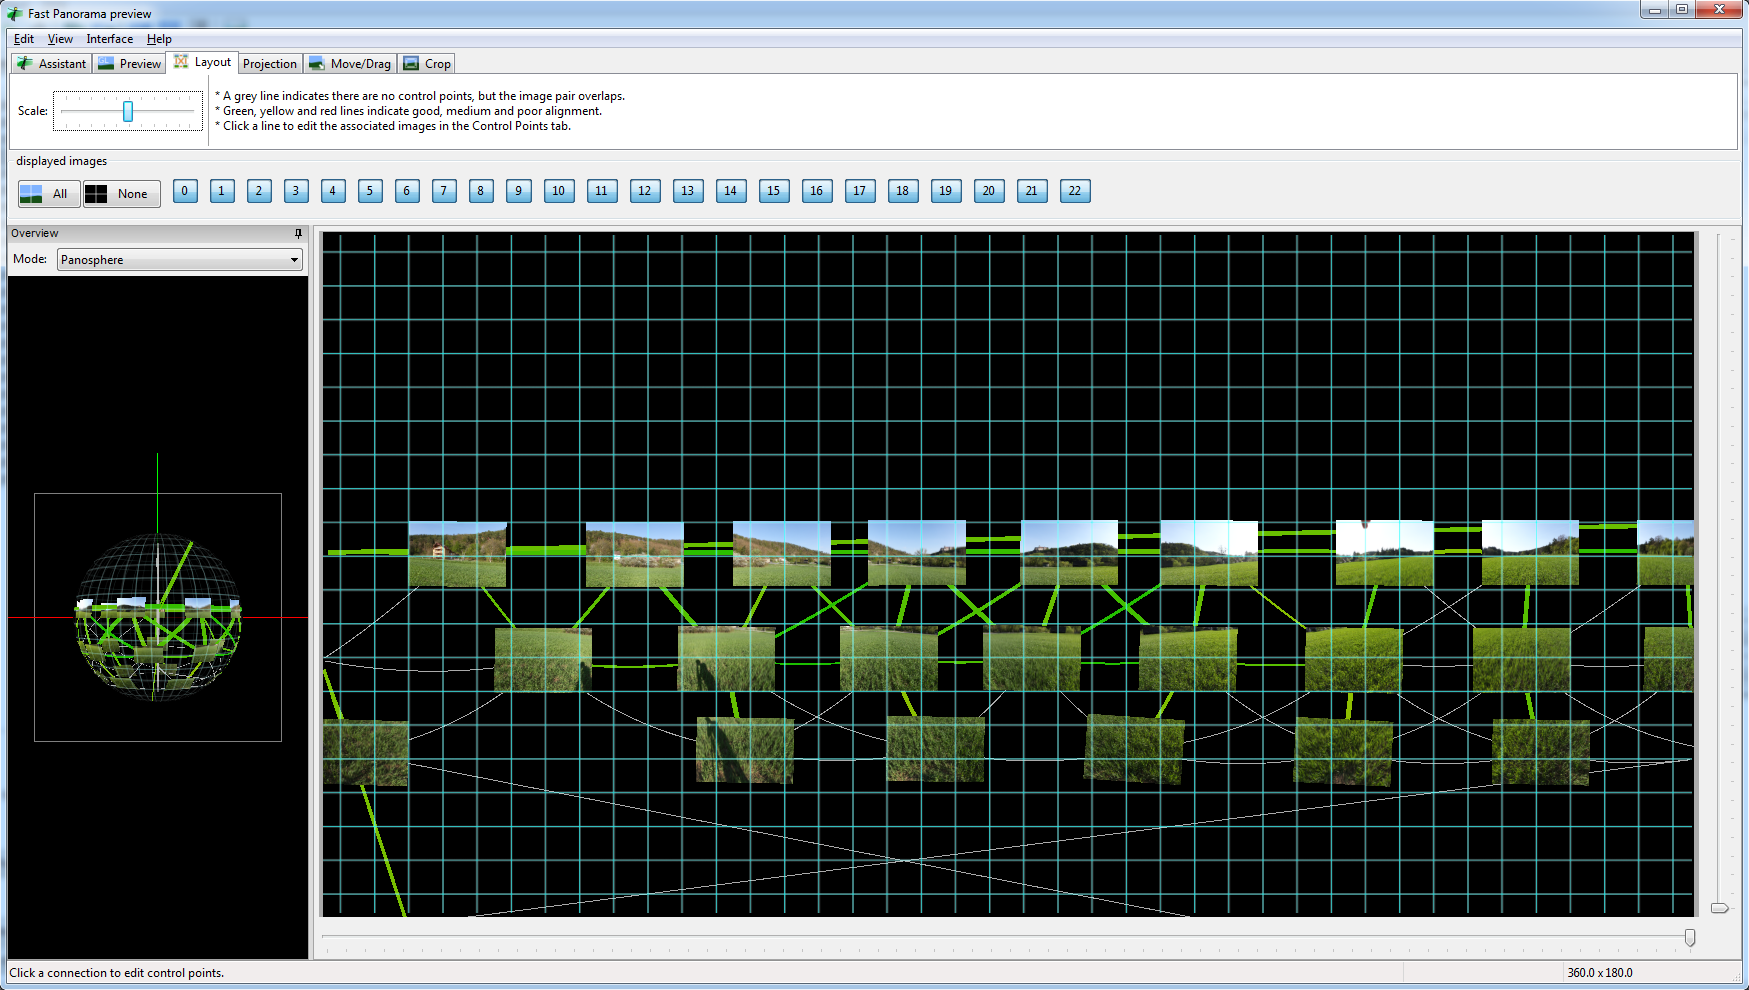
\includegraphics[width=\textwidth]{FastPreview.png}
    \caption{H\program{ugin}'s Fast Panorama Preview can be used to check which
      images are connected to its neighbours. Most important are good
      matches along the horizon, the images in the lower rows are
      clearly less important. If captured on a tripod, they should
      still match. }
  \label{fig:FastPanoPreview}
\end{figure}


\noindent
\colorbox{light-gray}{\fbox{\parbox[t]{0.975\linewidth}{
Basic rules to observe (use obvious inverses). 
%%%%%%%%%%%%%%%%%%%%%%%%%% DOUBLE-CHECK AGAIN!!!
\begin{itemize}
\item If image aligns well in azimuth but overshoots the grid to the
  right: Increase yaw accordingly (0.022°/pixel if image is 16384 pixels wide).
\item If the north end (left and right borders) is higher than the
  southern contact point: Increase pitch angle.
\item If north and south points are OK, but the western (right) half is
  higher than the eastern (left) half: Increase Roll angle.
\end{itemize}
The corrections required for pitch and roll may be surprisingly small!
}}}




Within a few rounds of adjustments, panorama creation, adding as layer
in the image editor, and comparing to the reference data, you should
achieve a match to fit your needs.

In case you have taken photographs in several rings but without a panorama tripod, you may have to
first align only the horizontal images (deselect the lower images to
exclude from optimisation), and when the horizon ring is aligned
perfectly, deactivate further optimisation in \program{Hugin} for those photos
while ``attaching'' (optimising) the lower photos. In \program{Hugin}'s \menu{Photos} tab,
select \menu{Optimise> Geometric> Custom Parameters}. This opens an
extra tab \menu{Optimiser}, where you can fine-tune your needs: Switch
off all variables for the photos in the horizon ring, and make sure
the lower photos fit in the preview after optimisation.

It may even help to define that the lower rows have been taken with a
different Lens, so the field of view and distortion settings of the
horizon row will be used as it had been found during the horizon-only
match.

By now you should have
enough experience what level of error may be acceptable for you.


\subsection{Artificial Panoramas}
\label{sec:landscapes:Artificial}

I have created a
website\footnote{\url{http://homepage.univie.ac.at/Georg.Zotti/php/panoCam.php}} where
you can enter geographical coordinates and download a file
\file{pano.kml}  which helps with image creation from \program{Google Earth}
imagery. Store this file for a site, let us call it
\landscape{MYPLACE}, into a new directory \file{GE\_MYPLACE} inside
your \file{landscapes} directory.

Store all scenes visible from the respective viewpoint
\landscape{MYPLACE} as picture into one common folder in your
\file{landscapes/GE\_MYPLACE} under the viewpoint name, e.g.,
\file{75-30.jpg}, which means 75 degrees from Nadir, azimuth 30
degrees.  Also, double-click the pano entry or the marker in \program{Google Earth} to open a window with the
basic content of your \file{landscape.ini}. Copy and paste from there
into a new file \file{landscape.ini} and adjust the obvious
entries. Complete as required with the entries described in
section~\ref{sec:landscapes:Spherical}.

On loading of the images, Hugin will not be able to detect any EXIF
lens data and ask you for the horizontal field of view. Enter 60
degrees, which is the standard value for \program{Google Earth}
screenshots\footnote{Note that if you work with \program{Google Earth Pro}, you
  can create different FoV!}.

The viewpoint names translate almost directly to the yaw and pitch
angles which you can enter in the image list in \program{Hugin}'s
\menu{Photos} tab. For example, switch to the \menu{Positions} display
on the right window edge in the \menu{Photo} tab, mark all images that
start with \file{25-} and assign a pitch angle of
$-90+\mathbf{25}=-65$. The second part of the names is directly the
azimuth.  In this case, don't run the optimizer, but you can
immediately set an output resolution and stitch
(see~\ref{sec:landscapes:stitching}). To get rid of the image
decorations (compass etc), apply masks\footnote{There is a wide
  overlap in the images to allow generous trimming.}. Postprocessing
steps are the same as for photo-panoramas: make sky invisible, crop,
etc.

It is also interesting to switch on the 3D buildings layer before
creating the images. If temples or other buildings are accurate, this
will give an even closer approximation to what would be visible
on-site. Note however that not every building will be modelled in
usable quality, and that usually vegetation is not included in the 3D
buildings layer. Also, if you are too close to buildings, they may be
cut away by the \emph{near clipping plane} of the rendering.

These images, based on \program{Google Earth} imagery and the SRTM
topographic model, seem usable as \emph{first rough approximation} to
a photo-based or surveyed panorama. Note that it is definitely not
accurate enough for representing nearby horizon features or critically
important mountain peaks, and please note that Google has image
copyright which at least requires you to acknowledge when displaying
these pictures.

\subsection{Nightscape Layer}
\label{sec:landscapes:landscapes:Nightscape}

Since version 0.13, Stellarium can simulate artificial illumination,
like streetlamps, bright windows, or the skyglow over cities. One way to
create this layer is to make 2 panorama series during the day and night
and process these in the same \program{Hugin} project to align those photos,
and then stitch two separate images by selecting either the daylight or the
nighttime shots. The night panorama has to be processed to remove
stars, airplanes, etc.

The other way is a simple layer overpainted in the image processing
program. As rough recommendation, use several layers to prepare this
feature:
\begin{itemize}
\item Put a semitransparent black layer over your daylight image, this
  helps you to place your painted pixels.
\item Paint windows, street lamps, signs, \ldots. You may apply a
  layer style to produce some glow.
\item To draw an impression of more light in the atmosphere (city
  skyglow), use a gradient with some brownish color. Generally the
  color depends on the appropriate mix of city lights (sodium, mercury
  vapour, etc.). Note that on the city outskirts a simple vertical
  gradient will not work, towards the city the horizon is much
  brighter. Use a huge but weak brush to make a more spotty sky.
\item Use the existing landscape as template for the layer mask for
  this gradient sky layer. (You want to hide skyglow by leaves in the
  foreground!)
\item If you want to add only a few lights to an \file{old\_style}
  landscape, you need to provide only the panels showing those
  lights. Just load a side panel for reference, place a new layer on
  top, and paint the lights on windows, lamps etc. There is no light
  option for the ground texture. This makes \file{old\_style}
  landscapes best suited for localized light pollution, not city
  skyglow.
\end{itemize}

The resulting image is then declared in the \var{maptex\_illum} line
of \file{landscape.ini}. Try also to balance the global strength of
light pollution with the \var{light\_pollution} key, and a probable
minimal brightness with the \var{minimal\_brightness} key.

Try to match the visual appearance, not necessarily what photographs
may have recorded. E.g., the \landscape{Grossmugl} sky shows horizon
glow mostly towards the city of Vienna, where long-time exposures may
already be saturated.

The possibilities seem limited only by your time and skills!

\section{Other recommended software}
\label{sec:landscapes:otherSoftware}

Here is a short collection of other useful programs for (panorama)
image manipulation and other tasks on Windows.


\subsection{IrfanView}
\label{sec:landscapes:IrfanView}

\program{IrfanView} is a free image viewer for Windows with many
options. It can show almost any image format, including several camera
RAW formats, in windowed and full-screen mode. It is definitely
preferrable over any image viewer built into Windows. Unfortunately
however, it has no panorama viewer function!

\subsection{FSPViewer}
\label{sec:landscapes:FSPViewer}

\program{FSPViewer}\footnote{Further details are available on its home
  page \url{http://www.fsoft.it/FSPViewer/}.} by Fulvio
Senore is an excellent panorama viewer for equirectanglar
images. Images centered along the horizon can be viewed directly,
while settings for images with different minimum and maximum angles,
as well as ``hotspots'' (similar to hyperlinks) which move to
neighboring panoramas, can be configured in an \file{.FSV} text file
like figure~\ref{fig:FSPexample}.


\begin{figure}[h]\centering
\begin{configfile}
ImageName=Horizon_Rosenburg.jpg
WindowTitle=Horizon_Rosenburg 
hFov=70 
#Formula: HP=100*(h/2-upper)/(lower-upper) in Hugin crop, or
#         HP=100*zeroRow/imgHeight 
HorizonPosition=33.8
\end{configfile}
\caption{FSP configuration file (example)}
\label{fig:FSPexample}
\end{figure}

\subsection{Clink}
\label{sec:landscapes:clink}

\program{Clink}\footnote{\url{http://mridgers.github.io/clink/}} is a command
line enhancement for Windows developed by Martin Ridgers. If you have
ever worked under a Linux \program{bash}-like command line, you will
easily feel that Windows' \program{cmd.exe} is extremely limited. \program{Clink}
provides several useful features, most notably a really usable
command-line completion. It is not essential for our tasks, but a
general improvement of usability of the Windows command line which
else has not caused me any trouble.

\subsection{Cygwin}
\label{sec:landscapes:cygwin}

Compared to Linux, the command line of Windows can be a humbling experience. None of
the wonderful helpers taken for granted on Linux are
available. \program{Cygwin}\footnote{\url{https://cygwin.com/index.html}}
provides a command line console with \program{bash} shell and all the
niceties like \program{make}, \program{awk}, \program{sed}, etc.\ which seem
essential for routine work.  If you are used to Linux tools, use
inline scripts in your \file{Makefile}s and need more than \program{Clink} can
offer, you should install \program{Cygwin}.

\subsection{GNUWin32}
\label{sec:landscapes:GNUwin32}

Alternative to \program{Cygwin}, several of those nice tools (\program{sed},
\program{awk} etc.) have also been made available as standalone commands
for Windows. If you don't need the inline scripting capabilities in
\file{Makefile}s which you would get from \program{Cygwin} but just want to call
\program{awk} or \program{sed} inside your \cmd{.BAT} scripts, maybe this is enough.


%%% Local Variables: 
%%% mode: latex
%%% TeX-master: "guide"
%%% End: 


%% Stellarium User Guide

\chapter{Deep-Sky Objects}
\label{ch:DSO}


Since version 0.10.0 Stellarium uses the ``json'' cataloguing system
of configuring textures. At the same time the Simbad online catalogue
was added to the search feature, making the catalog somewhat redundant
and used now only as a first search point or if there is no internet
connection.

If the object has a name (not just a catalogue number), you should add
one or more records to the \file{.../nebulae/default/names.dat} file
(where \file{...} is either the installation directory or the user
directory). See section~\ref{sec:dso:modifyingNamesDat} Modifying \file{names.dat}
for details of the file format.

If you wish to associate a texture (image) with the object, you must 
add a record to the \file{.../nebulae/default/textures.json} file. See
section~\ref{sec:dso:modifyingTexturesJson} for details of the file format.


\section{Stellarium DSO Catalog}
\label{sec:dso:catalog}

Stellarium's DSO Catalog contains over 14000 objects and is available
for end users as collection of files:

\begin{longtabu} to \textwidth {lX}
%\emph{File} & \emph{Description}\\
\file{catalog.txt} &Stellarium DSO Catalog in ASCII format for editing data\\
\file{catalog.dat} &Stellarium DSO Catalog in binary format for usage within Stellarium\\
\file{names.dat}   &List of proper names of the objects from file \file{catalog.dat}
\end{longtabu}

ASCII file can be converted into binary format through enabling an option in the file \file{config.ini} (See \ref{sec:ConfigurationFile}):
\begin{configfile}
[devel]
convert_dso_catalog = true
\end{configfile}

The file \file{catalog.txt} should be put into the directory
\file{.../nebulae/default/}.

Stellarium DSO Catalog contains data and supports the designations for
follow catalogues:

\begin{description}[align=right,labelwidth=2cm]
\item[\textbf{NGC}]  New General Catalogue 
\item[\textbf{IC}] Index Catalogue 
\item[\textbf{M}] Messier Catalog
\item[\textbf{C}] Caldwell Catalogue 
\item[\textbf{B}] Barnard Catalogue~\cite{1927cdos.book.....B} 
\item[\textbf{Sh2}] Sharpless Catalogue~\cite{1959ApJS....4..257S} 
\item[\textbf{VdB}] Van den Bergh Catalogue of reflection nebulae~\cite{1966AJ.....71..990V} 
\item[\textbf{RCW}]  A catalogue of H$\alpha$-emission regions in the southern Milky Way~\cite{1960MNRAS.121..103R} 
\item[\textbf{LDN}]  Lynds' Catalogue of Dark Nebulae~\cite{1962ApJS....7....1L} 
\item[\textbf{LBN}]  Lynds' Catalogue of Bright Nebulae~\cite{1965ApJS...12..163L} 
\item[\textbf{Cr}] Collinder Catalogue~\cite{1931AnLun...2....1C} 
\item[\textbf{Mel}]  Melotte Catalogue of Deep Sky Objects~\cite{1915MmRAS..60..175M} 
\item[\textbf{PGC}]  HYPERLEDA. I. Catalog of galaxies\footnote{The PGC and UGC catalogues have a partial support}
\item[\textbf{UGC}]  The Uppsala General Catalogue of Galaxies
\item[\textbf{Ced}]  Cederblad Catalog of bright diffuse Galactic nebulae~\cite{1946MeLuS.119....1C}
\end{description}

Cross-index data for Stellarium DSO Catalog is partially obtained from ``Merged catalogue of reflection nebulae''~\cite{2003A&A...399..141M}.

\subsection{Modifying catalog.dat}
\label{sec:dso:modifyingCatalog.dat}

This section describes the inner structure of the files \file{catalog.dat}
(binary format) and \file{catalog.txt} (ASCII format).
Stellarium can convert ASCII file into the binary format file for faster usage
within the program.

Each line contains one record, each record consisting of the following
fields with \emph{tab} char as delimiter:

\begin{longtabu} to \textwidth {l|l|X}
\toprule
\emph{Column} & \emph{Type} & \emph{Description}\\\midrule
 1 & integer & Deep-Sky Object Identificator\\
 2 & float   & RA (decimal degrees)\\
 3 & float   & Dec (decimal degrees)\\
 4 & float   & B magnitude\\
 5 & float   & V magnitude\\
 6 & string  & Object type (See section~\ref{sec:dso:types} for details).\\
 7 & string  & Morphological type of object\\
 8 & float   & Major axis size or radius (arcmin)\\
 9 & float   & Minor axis size (arcmin)\\
10 & integer & Orientation angle (degrees)\\
11 & float   & Redshift\\
12 & float   & Error of redshift\\
13 & float   & Parallax (mas)\\
14 & float   & Error of parallax (mas)\\
15 & float   & Non-redshift distance (\Mpc\ for galaxies, \kpc\ for other objects)\\
16 & float   & Error of non-redsift distance (\Mpc\ for galaxies, \kpc\ for other objects)\\
17 & integer & NGC number (New General Catalogue)\\
18 & integer & IC number (Index Catalogue)\\
19 & integer & M number (Messier Catalog)\\
20 & integer & C number (Caldwell Catalogue)\\
21 & integer & B number (Barnard Catalogue)\\
22 & integer & Sh2 number (Sharpless Catalogue)\\
23 & integer & VdB number (van den Bergh Catalogue of reflection nebulae)\\
24 & integer & RCW number (A catalogue of H$\alpha$-emission regions in the southern Milky Way)\\
25 & integer & LDN number (Lynds' Catalogue of Dark Nebulae)\\
26 & integer & LBN number (Lynds' Catalogue of Bright Nebulae)\\
27 & integer & Cr  number (Collinder Catalogue)\\
28 & integer & Mel number (Melotte Catalogue of Deep Sky Objects)\\
29 & integer & PGC number (HYPERLEDA. I. Catalog of galaxies); partial\\
30 & integer & UGC number (The Uppsala General Catalogue of Galaxies); partial\\
31 & string  & Ced number (Cederblad Catalog of bright diffuse Galactic nebulae)\\
\bottomrule
\end{longtabu}

\subsubsection{Types of Objects}
\label{sec:dso:types}

Possible values for type of objects in the file \texttt{catalog.dat}.

\begin{longtabu} to \textwidth {l|X}
\toprule
\emph{Type} & \emph{Description}\\\midrule
G   & Galaxy\\
GX  & Galaxy\\
AGX & Active Galaxy\\
RG  & Radio Galaxy\\
IG  & Interacting Galaxy\\
GC  & Globular Cluster\\
OC  & Open Cluster\\
NB  & Nebula\\
PN  & Planetary Nebula\\
DN  & Dark Nebula\\
RN  & Reflection Nebula\\
C+N & Cluster associated with nebulosity\\
HII & HII Region\\
SNR & Supernova Remnant\\
BN  & Bipolar Nebula\\
EN  & Emission Nebula\\
SA  & Stellar Association\\
SC  & Star Cloud\\
CL  & Cluster\\
IR  & Infra-Red Object\\
QSO & Quasar\\
Q?  & Possible Quasar\\
ISM & Interstellar Matter\\
EMO & Emission Object\\
LIN & LINEAR-type Active Galaxies\\
BLL & BL Lac Object\\
BLA & Blazar\\
MOC & Molecular Cloud\\
YSO & Young Stellar Object\\
PN? & Possible Planetary Nebula\\
PPN & Protoplanetary Nebula\\
$\ast$ & Star\\
$\ast\ast$ & Double Star\\
MUL & Multiple Star\\
\emph{empty} & Unknown type, catalog errors, \emph{Unidentified Southern Objects} etc.\\
\bottomrule
\end{longtabu}

\subsection{Modifying names.dat}%\label{modifying-names.dat}
\label{sec:dso:modifyingNamesDat}

Each line in the file \file{names.dat}  contains one record. A record
relates an extended object catalogue number (from \file{catalog.dat})
with a name. A single catalogue number may have more than one record in
this file.

The record structure is as follows:

\begin{longtabu} to \textwidth {l|l|l|X}
\toprule
\emph{Offset} & \emph{Length} & \emph{Type} & \emph{Description}\\
\midrule
0  &  5 & \%5s & Designator for catalogue (prefix)\\
5  & 15 & \%d  & Identificator for object in the catalog\\
20 & 60 & \%s  & Proper name of the object (translatable)\\
\bottomrule
\end{longtabu}

If an object has more than one record in the file \file{names.dat},
the last record in the file will be used for the nebula label.

\subsection{Modifying textures.json}%\label{modifying-textures.json}
\label{sec:dso:modifyingTexturesJson}

This file is used to describe each nebula image. The file structure
follows the JSON format, a detailed description of which may be found
at \url{www.json.org}. The \file{textures.json} file which ships with
Stellarium has the following structure:

%% TODO: GZ notes 2016-04 It seems there is some overdocumentation here, some entries seem to repeat in this list. FIX THAT!

\begin{description}
\item[serverCredits (optional)] a structure containing the following
  key/value pairs:

  \begin{description}
  \item[short] a short identifier of a server where the json file is found, e.g. ``ESO''
  \item[full]  a longer description of a server, e.g. ``ESO Online Digitised Sky Survey Server''
  \item[infoURL] a URL pointing at a page with information about the server
  \end{description}
\item[imageCredits] a structure containing the same parts as a
  serverCredits structure but referring to the image data itself
\item[shortName] an identifier for the set of images, to be used inside Stellarium
\item[minResolution] minimum resolution, applies to all images in the set,
  unless otherwise specified at the image level
\item[maxBrightness] the maximum brightness of an image, applies to all
  images in the set, unless otherwise specified at the image level
\item[subTiles] a list of structures describing indiviual image tiles, or
  referring to another json file. Each subTile may contain:

  \begin{description}
  \item[minResolution]
  \item[maxBrightness]
  \item[worldCoords]
  \item[subTiles]
  \item[imageCredits]
  \item[imageUrl]
  \item[textureCoords]
  \end{description}
\item[shortName] (name for the whole set of images, e.g. ``Nebulae'')
\item[miniResolution] (applies to all images in set)
\item[alphaBlend] (applies to all images in set)
\item[subTiles] list of images. Each image record has the following properties:

  \begin{description}
  \item[imageCredits] (itself a list of key/pairs)
  \item[imageUrl] (e.g. file name)
  \item[worldCoords] (a list of four pairs of coordinates representing the corners of the image)
  \item[textureCoords] (a list of four pairs of corner descriptions. i.e. which is top left of image etc)
  \item[minResolution] (over-rides file-level setting)
  \item[maxBrightness]
  \end{description}
\end{description}

Items enclosed in Quotation marks are strings for use in the program.
Syntax is extremely important. Look at the file with a text editor to
see the format. Items in \textless{}\textgreater{} are user provided
strings and values to suit the texture and source.

\begin{configfile}[\footnotesize]
{
  "imageCredits"  : { "short" : "<author name>" , 
                      "infoUrl" : "http://<mysite.org>" 
                    }, 
  "imageUrl"      : "<myPhoto.png>",
  "worldCoords"   : [[[ X0, Y0], [ X1, Y1], [ X2, Y2], [ X3, Y3] ]], 
  "textureCoords" : [[[ 0,0],[1,0],[1,1],[0,1]]], 
  "MinResolution" : 0.2148810463,
  "maxBrightness" : <mag>
},
\end{configfile}

where 

\begin{description}
\item[worldCoords] Decimal numerical values of the J2000 coordinates (RA and dec both in degrees) of the corners of the texture. These values are usually given to 4 decimal places.
\item[textureCoords]  Where 0,0 is South Left, 1,0 the South Right, 1,1 North Right, 0,1 North Left corners of the texture.
\item[MinResolution] UNDOCUMENTED VALUE! Sorry!%% TODO FIXME!
\item[maxBrightness] total object brightness, magnitude 
\end{description}


Calculating of the coords of the corners of the images (plate solving) is
a time consuming project and needs to be fine tuned from the screen
display. As most images will be two dimensional, display on a spherical
display will limit the size to about 1 degree before distortion becomes
evident. Larger images should be sectioned into a mosaic of smaller
textures for a more accurate display.

\section{Adding Extra Nebulae Images}%\label{adding-extra-nebulae-images}
\label{sec:dso:adding_images}
\sectionauthor*{Barry Gerdes}

\subsection{\texorpdfstring{Preparing a photo for inclusion to the \file{textures.json} file}{Preparing a photo for inclusion to the textures.json file}}
\label{sec:dso:preparing-a-photo}

\begin{figure}[h]
\centering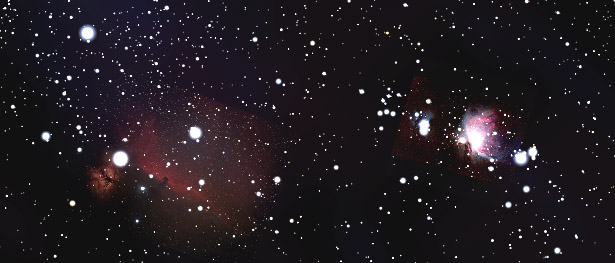
\includegraphics[width=\textwidth]{nebula-display}
\caption{Screen shot of nebula images displayed in Stellarium}
\label{fig:dso:preparing-a-photo}
\end{figure}

The first step is to take a photo of the object you wish to display in
Stellarium. When you have the picture you will need to align it with
the equatorial coordinate system so that north is directly up and not
inverted side to side or up and down as can happen with photos taken
with a diagonal mirror in the path. Next you will need to crop the
picture, setting the main feature at the centre and making the cropped
size a factor of $2^n$ eg. 64, 128, 256, 512, 1024 or 2048 pixels
square (or elongated like 512x1024).  If this requirement is not met,
your textures may not be visible, or graphics performance may be
seriously impacted. Textures larger than 2048 may only be supported on
high-end hardware. Images must be in PNG format.  When cropping, make
sure you leave at least six prominent background stars.

The next step is to process your photo to make the background
black, really black. This will ensure that your background will meld with the
Stellarium background and not be noticed as gray square. Suitable programs to do all
this are \program{The GIMP}\footnote{free in keeping with the Stellarium spirit; available from \url{http://www.gimp.org}} or
\program{Photoshop} if you can afford it.

When you have your image prepared you will need to plate solve it using
at least 6 known GSC stars that can be identified. That is why the
cropping with plenty of stars was necessary. When the plate is solved
you will need to find the J2000 coordinates of the corners and convert
them to decimal values to form the world coordinates in the
\file{textures.json} file.

\begin{figure}[htb]
\centering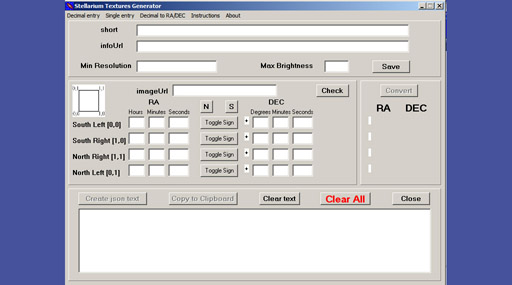
\includegraphics[width=\textwidth]{EQ-Decimal.jpg}
\caption{\program{Stellarium Textures Generator}: A program to convert Equatorial coordinates into decimal
form and write a \texttt{textures.json} insert}
\label{fig:dso:STGen}
\end{figure}

The program \program{Stellarium Textures Generator} by Peter Vasey (Fig.~\ref{fig:dso:STGen}) can convert the corner coordinates of a
texture found in your plate solving program into decimal values and write an
insert for the \file{textures.json} file.\footnote{It is available as a freebee
from
\url{http://www.madpc.co.uk/~peterv/astroplover/equipnbits/Stellariumtextures.zip}.}

\begin{figure}[ht]
\centering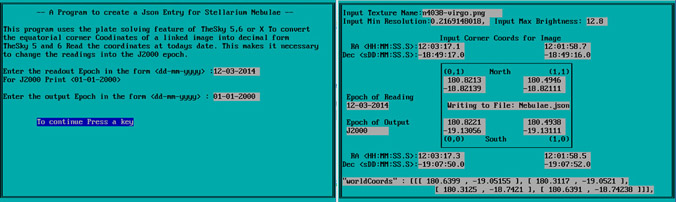
\includegraphics[width=\textwidth]{pix-4.jpg}
\caption{\program{ReadDSS}: A program to write a \file{textures.json} insert with epoch manipulation.}
\label{fig:dso:ReadDSS}
\end{figure}

There is another program, \program{ReadDSS} (Fig.~\ref{fig:dso:ReadDSS}), written by Barry Gerdes in Qb64(gl), that will perform the same
task but allows manipulation of the epochs.\footnote{
\url{http://barry.sarcasmogerdes.com/stellarium/uploads/writejsoninsert.zip}}

\subsection{Plate Solving}%\label{plate-solving}
\label{sec:dso:plateSolving}

Suitable programs that can accept your picture and calculate its corner
coordinates are hard to find. I have only found one that suits our
purpose and it is another expensive planetarium program, \program{TheSky X Pro}.
However the older versions \program{TheSky 5} and \program{6 Pro} will also do the job if
suitably configured, although I could not solve the test program with 
\program{TheSky 6} that uses the same procedure as \program{TheSky 5}.

These programs have a link feature that can match your photo to the
selected area of the screen and superimpose it on the display with a box
around your photo provided it can match at least 6 stars from the GSC
that is included with the program. When this is fitted you can read the
corner coordinates of your texture in the Status bar by selecting them
with a mouse. \program{TheSky X} can read these coordinates in J2000 values and
uses textures in the FITS format, but the earlier programs only read the
coordinates of the current program date. To read the J2000 coordinates
it is necessary to re-start the program with the date set to 1-1-2000.

To add the picture to \program{TheSky 5} you need first make a mono 8 bit version
of the photo and place it on the clipboard. Run \program{TheSky} and centre on the
object centre. Look in the \menu{Tools} menu for the \menu{image} link and select
\menu{setup}. Tick \menu{show image frame} to put a frame around the image.

Paste the clipboard image on the display and use the zoom and position
controls to get it as close to the size and position as possible by
visually matching stars. Go to the menu again and click on \menu{link wizard}.
If you have been successful the window will show the number of stars
matched and the option to \menu{accept} or \menu{continue}. Accept and you will now
see all the matched stars have overlaid the picture. You can now read
off the corner coordinates from the status bar starting at the bottom
(south) left and continuing counterclockwise to the top (north) left.

\subsection{\texorpdfstring{Processing into a \texttt{textures.json} insert}{Processing into a textures.json insert}}%\label{processing-into-a-textures.json-insert}

Place your image in the \file{*.png} format in the
\file{.../nebulae/default/} folder. Ensure that the name matches the
\file{textures.json} entry.

Once you have the corner coordinates of your photo you can add them to
the decimal converter program and it will write an insert
\file{nebula.json} as a text file that you can paste directly into the
\file{textures.json} file that is in the \file{.../nebulae/default/}
folder.

Save the \file{textures.json} file with the new insert and run
Stellarium. Find the object in the \key{F3} Object selection window and slew to
it. Your image should be there and with a bit of luck it will nicely
overlay the stars in Stellarium. However this only rarely
happens, so a little bit of tweaking of the JSON \parameter{worldcoords} will be
needed to get a perfect match. Select equatorial mode (\guibutton{0.6}{bt_coord_type} or \keys{\ctrl+M}).
This will show the area with north up. Select each corner in sequence
and make small changes to the coordinates. Restart Stellarium each time
and check if you have moved into the right direction. Continue with each
corner until all the stars match. With a little bit of practice this
will be done in about 10 minutes.


%%% Local Variables: 
%%% mode: latex
%%% TeX-master: "guide"
%%% End: 
 %% Maybe DSO is more a reference chapter? --> Appendix in this case? Or split?
%% Part of Stellarium User Guide 0.15+
%% History:
%% 2016-04-17 New chapter.


\chapter{Adding Sky Cultures}
\label{ch:SkyCultures}
\chapterauthor*{Georg Zotti}

Stellarium comes with a nice set of skycultures. For ethnographers or
historians of science it may be a worthwile consideration to
illustrate the sky culture of the people they are studying. It is not
very hard to do so, but depending on your data, may require some
skills in image processing. 

Some features regarding translation and multilinguality have evolved
over the years, and not all skycultures currently included in
Stellarium adhere to the standards described in the following
sections. If you add a new skyculture, please do so for an optimal
result!




In the Stellarium program folder you can see a folder
\file{skycultures}. Let us assume you work on Windows and want to create a
new Skyculture, say, \emph{myCulture}.


You can take the \file{inuit} directory as template to start with. Just copy the folder 
\file{C:\textbackslash{}Program Files\textbackslash{}Stellarium\textbackslash{}skycultures\textbackslash{}inuit} to
\file{C:\textbackslash{}Users\textbackslash{}[YOU]\textbackslash{}AppData\textbackslash{}Roaming\textbackslash{}Stellarium\textbackslash{} skycultures\textbackslash{}myculture}

In the folder you see image files for the constellation artwork, and all
other files with various extensions are text files. 


\section{Basic Information}
\label{sec:skycultures:info.ini}


In \file{myculture\textbackslash{}info.ini}, change the entries to 
\begin{configfile}
[info]
name=myCulture
author=me
\end{configfile}

\noindent (or what seems best for you). The name is used for the list entry in
the Starlore tab in the View dialog (see \ref{sec:gui:view:starlore}).


\section{Skyculture Description Files}
\label{sec:skycultures:description}


In order to have translated texts we have files
\file{description.<LANG>.utf8}, where \file{<LANG>} is the two-letter
ISO~639-1 language code, or its extension which contains language and
country code, like \file{pt\_BR} for Brazilian Portuguese. A minimum
skyculture must contain the file \file{description.en.utf8}, this is
\texttt{en=english} text with optional HTML tags for sections, tables,
etc. You can also have embedded images in the HTML (your book cover?
Views of sacred landscapes/buildings/artwork/\ldots?), just make them
PNG format please. The length of the description texts is not limited,
you have room for a good description, tables of names/translations,
links to external resources, whatever seems suitable. When you started
from a copied skyculture, delete the other \file{description.*.utf8}
files.

If you can provide other languages supported by Stellarium, you can
provide translations yourself, else Stellarium translators \emph{may}
translate the English version for you. (It may take years though.) The file
ending \file{.utf8} indicates that for special characters like ÄÖÜßáé
you should use UTF8 encoding. If you write only English/ASCII, this may not
be relevant.

\section{Constellation Names}
\label{sec:skycultures:constellations}

The native constellations are listed in
\file{constellation\_names.eng.fab}. It consists of 3 simple columns:
Abbreviation(or just a serial number), native name, and english
translation. The writing \texttt{\_("name")} allows automatic
translation of the English strings to other languages. These strings
will be used as constellation labels.

The first column (abbreviation) in the Western sky culture provides
the canonical 3-letter abbreviation for constellations as used by the
International Astronomical Union. Such abbreviations may not be
available for the skyculture you are working with, so you must invent
your own. These abbreviations are used as keys in the other files, so
they must be unique within your skyculture.
It is not necessary to have 3-letter keys. 

The keys can be displayed on screen when labels are requested in the
Starlore GUI (section~\ref{sec:gui:view:starlore}). If you want to prevent
certain abbreviations from being displayed, let them start with a
dot. See the effect in the \file{Western (H.A.Rey)} skyculture: In
\menu{Abbreviated} mode, only the official abbreviations are
displayed. In \menu{Native} mode, the second column of
\file{constellation\_names.eng.fab} is shown. Only with setting
\menu{Translated}, the text translated from the text shown in the
third column is shown. If your skyculture is a variant of the Western
skyculture, please use the canonical Latin names, they have all been translated already.

If your skyculture is not a variant of the generally known Western
skyculture, please include an English translation to the name given in
the native language. Else translators will not be able to translate
the name. See a good example in the Mongolian skyculture.

\section{Star Names}
\label{sec:skycultures:starnames}

The file \file{star\_names.fab} contains a list of HIP catalogue
numbers and common names for those stars. Each line of the file
contains one record of two fields (separated by the pipe character
(\texttt{|})) or three fields (first pair is separated by the 
pipe character (\texttt{|}) and last one separated by the space 
character). The first field is the Hipparcos catalogue number of the
star, the second is the common name of the star in a format that enables
translation support, the third is an optional list of references (see \ref{sec:skycultures:references})  
to source of the info about this name, e.g:
\begin{configfile}
# Piscis Austrinus (PsA)
113368|_("Fomalhaut") 1,2,6,11,12
113368|_("Thalim")
\end{configfile}

In the sample you can see 3 lines: the first line is comment, the 
second line has 3 fields and the third line has 2 fields. Both lines 
with data has the same Hipparcos number of the star --- \textit{Fomalhaut} is 
the well-known name of HIP 113368, \textit{Thalim} is an additional name 
of this star (not well-known name).

\section{Planet Names}
\label{sec:skycultures:planetnames}

The file \file{planet\_names.fab} contains a list of native names of
planets. Each line of the file contains one record of 3 fields,
separated by the white space or tab character. The first field is the
English name of the planet, the second is the native name of the
planet (can be in the native language, but please for maximum
utability use an english transliteration) and the third is the
translatable version of the native name of the planet (translated into
English). Here is an example from the Egyptian skyculture:

\begin{configfile}
Mars	"Horus-Desher"	_("Red Horus (Mars)")
\end{configfile}

\section{Deep-Sky Objects Names}
\label{sec:skycultures:dsonames}

\newFeature{V0.15.1} The file \file{dso\_names.fab} contains a list of native names of
deep-sky objects. The format of this file is similar of 
\file{star\_names.fab} format (see \ref{sec:skycultures:starnames}).
Each line of the file contains one record of two fields (separated 
by the pipe character (\texttt{|})) or three fields (first pair is 
separated by the pipe character (\texttt{|}) and last one separated 
by the space character). The first field is an identificator of 
deep-sky object, the second is the native name of the DSO in a 
format that enables translation support, the third is an optional 
list of references (see \ref{sec:skycultures:references}) to source 
of the info about this name, e.g:
\begin{configfile}
PGC 17223|_("Native name for LMC") 1,2,3
NGC 292  |_("Native name for SML") 1,3
NGC 292  |_("Small Magellanic Cloud")
\end{configfile}

\section{Stick Figures}
\label{sec:skycultures:stickfigures}



The modern-style stick figures are coded in \file{constellationship.fab}. Lines
look like:

\begin{configfile}
Abbr pairs pair1_star1 pair1_star2 pair2_star1 pair2_star2 ...
\end{configfile}
In this file,
\begin{description}
\item[Abbr] is the abbreviation defined in \file{constellation\_names.eng.fab}
\item[pairs] is the number of line pairs which follow.
\item[pairN\_starA] Hipparcos numbers for the stars which form the
  constellation stick figure. We need two entries per line, longer
  line segments are not supported. To find the HIP number, just have
  Stellarium open and click on the star in Stellarium while editing
  this file.
\end{description}

\section{Constellation Borders}
\label{sec:skycultures:borders}

The optional file \file{constellations\_boundaries.dat} includes data for the
border lines drawn between constellations.  The western constellations
have been given borders based on B1875.0 coordinates, and all
skycultures with names starting in \file{Western\_} use these borders
automatically.

The format for this file is a bit more dificult than the other files. It contains sections which may consist of multiple lines, of the format:

\begin{configfile}
N RA_1 DE_1 RA_2 DE_2 ... RA_N DE_N 2 CON1 CON2
\end{configfile}
where
\begin{description}
\item[N] number of corners
\item[RA\_n, DE\_n] right ascension and declination (degrees) of the corners in J2000 coordinates.
\item[2 CON1 CON2] legacy data. They indicated ``border between 2 constellations, CON1, CON1'' but are now only required to keep the format. %% TODO Assumptions by GZ while writing in 2016-04. 
\end{description}

\section{Constellation Artwork}
\label{sec:skycultures:artwork}

Constellation artwork is optional, but may give your skyculture the
final touch, if it requires artwork at all. E.g., H. A. Rey's variant
of the Western skyculture deliberately does not contain artwork.

Each constellation artwork is linked to 3 stars in its constellation. This
is programmed in the file \file{constellationsart.fab}. You have to write lines

\begin{configfile}
  Abbr image_name.png x1 y1 HIP1 x2 y2 HIP2 x3 y3 HIP3
\end{configfile}
where 
\begin{description}
\item[Abbr] is the abbreviation defined in \file{constellation\_names.eng.fab}
\item[image\_name.png] is the file name of your texture. It should be
  sized in a power of two, like $512\times512$, $1024\times2048$
  etc. Avoid dimensions larger than 2048, they are not supported on
  all systems. You can distort images to better exploit the pixels,
  the texture will be stretched back. The background of the artwork
  image must be absolutely black.
\item[x\textit{n}, y\textit{n}, HIP\textit{n}] pixel locations of the
  star in the constellation drawing (find those in any image editor)
  and HIP\textit{n} is the star number in the Hipparcos catalog, which
  you find when you click on the star in Stellarium.
\end{description}

In case the artwork is only available in a certain projection (e.g.,
an all-sky map), or is otherwise heavily distorted so that the match
is not satisfactory, you may have to reproject the image somehow. For
aligning, you should switch Stellarium to Stereographic projection for
optimal results.

You don't have to shutdown and restart Stellarium during
creation/matching, just switch skyculture to something else and back
to the new one to reload.

\section{Seasonal Rules}
\label{sec:skycultures:seasonal_rules}

File \file{seasonal\_rules.fab} (optional) contains possible seasonal rules for
the visibility of constellations. There is one rule per line. Each
rule contains three elements separated with white space (or tab
character): constellation ID, start of visibility (month) and end of
visibility (month), e.g:

\begin{configfile}
  Emu 6 3
\end{configfile}

\noindent This specifies that constellation Emu (abbreviated also as ``Emu'') is
visible only from June to March.
%% TODO: This feature may need rework. Where is it used?

\section{References}
\label{sec:skycultures:references}

\newFeature{V0.15.1} The file \file{reference.fab} contains a list of sources information. 
Each line of the file contains one record of 3 fields,
separated by the pipe character (\texttt{|}) --- number of source, 
description of source and optional URL, e.g.:

\begin{configfile}
9|Kruger 60|https://en.wikipedia.org/wiki/Kruger_60
\end{configfile}

\section{Publish Your Work}
\label{sec:skyculture:publish}

If you are willing to let other users enjoy the result of your hard work (and we
certainly hope you do!), when you are done, please write a note in the
Forum or at Launchpad.  Please be prepared to put the imagery and text
under some compatible open-source license (Creative Commons). Else the
skyculture cannot be hosted by us.


%%% Local Variables: 
%%% mode: latex
%%% TeX-master: "guide"
%%% End: 


%----------------------------------------------------------------------------------------
%	PART III
%----------------------------------------------------------------------------------------
\part{Extending Stellarium}
\chapterimage{chapter-t3-bg} % Chapter heading image

\chapter{Plugins}
\label{ch:Plugins}

Starting with version 0.10.3, Stellarium's packages have included a steadily growing number of
plug-ins: Angle Measure, Compass Marks, Oculars, Telescope Control, Text
User Interface, Satellites, Solar System Editor, Historical Novae and 
Supernovae, Quasars, Pulsars, Exoplanets, Observability analysis, ArchaeoLines, Scenery3D, RemoteControl. All
these plug-ins are ``built-in'' in the standard Stellarium distribution
and don't need to be downloaded separately.

%% TODO: Are there still downloadable plugins?

\section{Enabling plugins}
\label{sec:Plugins:EnablingPlugins}

%\begin{figure}[h]
%\centering\includegraphics{sat_howto_01.jpg}
%\end{figure}

To enable a plugin:

\begin{enumerate}
\item Open the \textbf{Configuration dialog} (press \key{F2} or use
  the left tool bar button \guibutton[0.35]{0.1}{btd_config})
\item Select the \textbf{Plugins} tab
\item Select the plugin you want to enable from the list
\item Check the \textbf{Load at startup} option
\item Restart Stellarium
\end{enumerate}

\noindent If the plugin has configuration options, the
\textbf{configuration} button will be enabled when the plugin has been
loaded and clicking it will open the plugin's configuration
dialog. When you only just activated loading of a plugin, you must
restart Stellarium to access the plugin's configuration dialog.

\section{Data for plugins}
\label{sec:Plugins:DataForPlugins}

Some plugins contain files with different data, e.g., catalogs. JSON is a
typical format for those files and you can edit its content manually. Of
course, each plugin has a specific format of data for the own catalogs, and
you should read documentation for the plugin before editing of its catalog.

You can read some common instructions for editing catalogs of plugins
below. In this example we use file name \file{catalog.json} for
identification of catalog for a typical plugin.

You can modify the \file{catalog.json} files manually using a text
editor. \textbf{If you are using Windows, it is strongly recommended to
use an advanced text editor such as
Notepad++\footnote{\url{http://notepad-plus-plus.org/}} to avoid problems with
end-of-line characters.} (It will also color the JSON code and make it
easier to read.)

\textbf{Warning}: Before editing your \file{catalog.json} file, make a
backup copy. Leaving out the smallest detail (such as a comma or
forgetting to close a curly bracket) will prevent Stellarium from
starting.

As stated in section~\ref{sec:FilesAndDirectories}, the path to the
directory\footnote{This is a hidden folder, so in order to find it you
  may need to change your computer's settings to display hidden files
  and folders.} which contains \file{catalog.json} file is something
like:

\begin{description}
\item[Windows]
  C:\textbackslash Users\textbackslash\textbf{UserName}\textbackslash AppData\textbackslash Roaming\textbackslash Stellarium\textbackslash modules\textbackslash \textit{PluginName}
\item[Mac OS X]
  \textbf{HomeDirectory}/Library/Preferences/Stellarium/modules/\textit{PluginName}
\item[Linux and UNIX-like OS]
  \textasciitilde{}/.stellarium/modules/\textit{PluginName}
\end{description}



%%% Local Variables: 
%%% mode: latex
%%% TeX-master: "guide"
%%% End: 

%% Part of Stellarium User Guide
%% Status: 2015-12-30 Some parts collected from wiki.
%%         2016-04-05 GZ changed to have 1 chapter per plugin for a better structure. This file may be split up later. 
%% TODO: All plugins! And give a better structure than just by alphabet.
%%         2016-04-16 split plugin part to topical chapters.

\chapter{Interface Extensions}
\label{ch:plugins:Interfaces}

Most users will soon be familiar with the usual user interface. A few
plugins are available which extend the regular user interface with a
few small additions which are presented first.  However, some
applications and installations of Stellarium require completely
different user interfaces. Mostly, these serve to avoid showing the
user interface panels to an audience, be that in your astronomy club
presentations, a domed planetarium or in a museum installation.


\section{Angle Measure Plugin}
\label{sec:plugins:AngleMeasure}

\begin{quotation}\small
\noindent\emph{goes misty eyed}\\ 
I recall measuring the size of the Cassini Division when I was a student.
It was not the high academic glamor one might expect\ldots It was cloudy\ldots
It was rainy\ldots The observatory lab had some old scopes set up at one
end, pointing at a \emph{photograph} of Saturn at the other end of the
lab. We measured. We calculated. We wished we were in Hawaii. A picture
is worth a thousand words.
\end{quotation}

%\url{http://porpoisehead.net/images/plugin-angle-measure.jpg}

\noindent The Angle Measure plugin is a small tool which is used to measure the
angular distance between two points on the sky. 


%\subsection{Using the plugin}
%\label{sec:plugins:AngleMeasure:using}

\begin{enumerate}
\item Enable the tool by clicking the tool-bar button, or by pressing
  \key{\ctrl+A}. A message will appear at the bottom of the screen to
  tell you that the tool is active.
\item Drag a line from the first point to the second point using the
  left mouse button
\item To clear the measurement, click the right mouse button
\item To deactivate the angle measure tool, press the tool-bar button
  again, or press \key{\ctrl+A} on the keyboard.
\end{enumerate}

\noindent In the configuration dialog, you can configure if you want to have
distances given on the rotating sphere, or in horizontal
(alt-azimuthal) coordinates. You can also link one point to the
resting horizon, the other to the sky and observe how angles change.

\newpage

\section{Compass Marks Plugin}
\label{sec:plugins:CompassMarks}

%\url{http://porpoisehead.net/images/plugin-compass-marks.jpg}

Stellarium helps the user get their bearings using the cardinal point
feature -- the North, South, East and West markers on the horizon.
Compass Marks takes this idea and extends it to add markings every few
degrees along the horizon, and includes compass bearing values in
degrees.

When activated (see section~\ref{sec:Plugins:EnablingPlugins}), there
is a tool bar button \guibutton{0.6}{bt_compass_off} for toggling the
compass markings.  Note that when you enable compass marks, the
cardinal points will be turned off.

\begin{figure}[ht]\centering
\includegraphics[width=\textwidth]{compass-marks-plugin}
\caption{Markings of Compass Marks Plugin}
\label{fig:plugins:CompassMarks}
\end{figure}

%% TODO/FIXME?: The following is not true for current pre-0.15:
%You can have both active at once, but there is a small
%bug which means you have to press \key{Q} \emph{two times} to
%re-enable cardinal points after enabling the compass markings.


\newpage
\section{Equation of Time Plugin}
\label{sec:plugins:EquationOfTime}

%% The figure just reproduces most of the text. I (GZ) regard it not so necessary. 
%\begin{figure}[h]
%\includegraphics[width=\textwidth]{EquationOfTime-plugin.jpg}
%\caption{Interface of Equation of Time plugin}
%\label{fig:EqOfTime}
%\end{figure}

\begin{figure}[h]\centering
\includegraphics[width=.3\textwidth]{GZ_analemma_p1000}
\includegraphics[width=.3\textwidth]{GZ_analemma_p2000}
\caption{Figure-8 plots for Equation of Time, for years 1000 (left)
  and 2000 (right). These plots, often found on sundials, link solar
  declination (vertical axis) and its deviation at mean noon from the
  meridian, in minutes. Labeled dots indicate when the sun entered the
  respective Zodiacal sign (30\degree section of the
  ecliptic). Figures by Georg Zotti.}
\label{fig:EqOfTime}
\end{figure}


\noindent The Equation of Time plugin shows the solution of the equation of time. % (Fig.~\ref{fig:EqOfTime}).
This describes the discrepancy between two kinds of
solar time:
\begin{description}
\item[Apparent solar time] directly tracks the motion of the sun. Most sundials show this time.
\item[Mean solar time] tracks a fictitious ``mean'' sun with noons 24 hours apart. 
\end{description}

There is no universally accepted definition of the sign of the
equation of time. Some publications show it as positive when a sundial
is ahead of a clock; others when the clock is ahead of the sundial. In
the English-speaking world, the former usage is the more common, but
is not always followed. Anyone who makes use of a published table or
graph should first check its sign usage.

If enabled (see section~\ref{sec:Plugins:EnablingPlugins}), click on
the Equation of Time button \guibutton{0.6}{bt_EquationOfTime_72dpi}
on the bottom toolbar to display the value for the equation of time on
top of the screen.


\subsection{Section \big[EquationOfTime\big] in config.ini file}
\label{sec:plugins:EquationOfTime:config}

You can edit \file{config.ini} file by yourself for changes of the
settings for the Equation of Time plugin -- just make it carefully!

\begin{longtabu} to \textwidth {l|l|X}\toprule
\emph{ID}            & \emph{Type} & \emph{Description}\\\midrule
enable\_at\_startup  & bool & Display solution of the equation of time at startup of the planetarium\\\midrule
flag\_use\_ms\_format & bool & Set format for the displayed solution - minutes and seconds and decimal minutes\\\midrule
flag\_use\_inverted\_value & bool & Change sign of the equation of time \\\midrule
flag\_show\_button & bool & Enable displaying plugin button on the bottom toolbar\\\midrule
text\_color & R,G,B & Color of font for the displayed solution of the equation of time\\\midrule
font\_size & int & Font size for the displayed solution of the equation of time \\\bottomrule
\end{longtabu}



\newpage

\section{Field of View Plugin}
\label{sec:plugins:FieldOfView}

\begin{figure}[ht]\centering
\includegraphics[trim=0 55 0 0,clip,width=.52\textwidth]{FOV-plugin.jpg}
\caption{Configuration dialog of Field of View plugin}
\label{fig:plugins:FieldOfView}
\end{figure}

\noindent By default Stellarium uses smooth zooming via mouse wheel or
keyboard shortcuts. Some users may want stepwise zooming to fixed
values for field of view like in the \program{Cartes du
  Ciel}\footnote{SkyChart / Cartes du Ciel planetarium:
  \url{http://www.ap-i.net/skychart/en/start}} planetarium program,
and this plugin provides this feature. You can edit values and use the
keyboard for quick-setting of FOV. All values in degrees.

%\section{Using the Field of View plugin}
%\label{sec:plugins:FieldOfView:using}

\begin{enumerate}
\item Enable the tool by configuring it to ``Load at startup''.
\item Press shortkeys for quick changes of FOV.
\end{enumerate}

\subsection{Section \big[FOV\big] in config.ini file}
\label{sec:plugins:FieldOfView:config}

You can configure the plugin with its dialog (Fig.~\ref{fig:plugins:FieldOfView}) or edit
\file{config.ini} file by yourself for changes of the settings for the
Field of View plugin -- just make it carefully!

\begin{longtabu} to \textwidth {l|l|r|X}\toprule
\emph{ID} & \emph{Type} & \emph{Default} & \emph{Description}\\\midrule
fov\_quick\_0  & float & 0.5& Value of FOV for the shortcut \key{\ctrl+\Alt+0} \\\midrule
fov\_quick\_1  & float &180 & Value of FOV for the shortcut \key{\ctrl+\Alt+1} \\\midrule
fov\_quick\_2  & float & 90 & Value of FOV for the shortcut \key{\ctrl+\Alt+2} \\\midrule
fov\_quick\_3  & float & 60 & Value of FOV for the shortcut \key{\ctrl+\Alt+3} \\\midrule
fov\_quick\_4  & float & 45 & Value of FOV for the shortcut \key{\ctrl+\Alt+4} \\\midrule
fov\_quick\_5  & float & 20 & Value of FOV for the shortcut \key{\ctrl+\Alt+5} \\\midrule
fov\_quick\_6  & float & 10 & Value of FOV for the shortcut \key{\ctrl+\Alt+6} \\\midrule
fov\_quick\_7  & float &  5 & Value of FOV for the shortcut \key{\ctrl+\Alt+7} \\\midrule
fov\_quick\_8  & float &  2 & Value of FOV for the shortcut \key{\ctrl+\Alt+8} \\\midrule
fov\_quick\_9  & float &  1 & Value of FOV for the shortcut \key{\ctrl+\Alt+9} \\\bottomrule
\end{longtabu}

\newpage

\section{Pointer Coordinates Plugin}
\label{sec:plugins:PointerCoordinates}


\begin{figure}[th]\centering
\includegraphics[trim=0 140 0 0,clip,width=.85\textwidth]{PointerCoordinates-plugin.jpg}
\caption{Interface of Pointer Coordinates plugin}
\label{fig:PointerCoordinates}
\end{figure}

\noindent The Pointer Coordinates plugin shows the coordinates of the mouse pointer.
If enabled, click on the plugin button \guibutton{0.6}{bt_PointerCoordinates_Off} on the bottom toolbar to display the coordinates of the mouse pointer.

\subsection{Section \big[PointerCoordinates\big] in config.ini file}
\label{sec:plugins:PointerCoordinates:config}

You can edit \file{config.ini} file by yourself for changes of the
settings for the Pointer Coordinates plugin -- just make it carefully!

\begin{longtabu} to \textwidth {l|l|X}\toprule
\emph{ID}            & \emph{Type} & \emph{Description}\\\midrule
enable\_at\_startup  & bool & Enable displaying coordinates of the mouse pointer at startup of the plugin\\\midrule
flag\_show\_button   & bool & Enable showing the button of the plugin on bottom toolbar\\\midrule
text\_color          & R,G,B & Color for text with coordinates of the mouse pointer \\\midrule
font\_size           & int & Font size for the displayed coordinates of the mouse pointer \\\midrule
current\_displaying\_place  & string & Specifies the place of displaying coordinates of the mouse pointer. \textit{Possible values}: \keymap{TopRight}, \keymap{TopCenter}, \keymap{RightBottomCorner}, \keymap{Custom}. \textit{Default value}: \keymap{TopRight}. \\\midrule
current\_coordinate\_system & string & Specifies the coordinate system. \textit{Possible values}: \keymap{RaDecJ2000}, \keymap{RaDec}, \keymap{HourAngle}, \keymap{Ecliptic}, \keymap{AltAzi}, \keymap{Galactic}. \textit{Default value}: \keymap{RaDecJ2000}. \\\midrule
custom\_coordinates  & int,int & Specifies the screen coordinates of the custom place for displaying coordinates of the mouse pointer \\\midrule
flag\_show\_constellation &bool& Add the 3-letter IAU abbreviation for the constellation the mouse pointer sits in \cite{1987PASP...99..695R}.\\\bottomrule
\end{longtabu}




\newpage

\section{Text User Interface Plugin}
\label{sec:plugins:TextUserInterface}

%\url{http://porpoisehead.net/images/plugin-tui.jpg}

This plugin re-implements the ``TUI'' of the pre-0.10 versions of
Stellarium, an unobtrusive menu used primarily by planetarium system
operators to change settings, run scripts and so on.

Given that color configuration for lines and texts cannot be found
elsewhere, an interesting part for general use (at least for extended
configuration sessions) is the way to interactively select colors in
this menu.

A full list of the commands for the TUI plugin is
given in section~\ref{sec:plugins:TUI:commands}. 

\subsection{Using the Text User Interface}
\label{sec:plugins:TUI:using}

\begin{enumerate}
\item Activate the text menu using the \key{\Alt+T} key.\footnote{This
    used to be hard-coded to \key{M} before version 0.15, but
    \key{\Alt+T} is better to remember as it runs parallel with
    \key{\ctrl+T} for switching the GUI panels, and frees up \key{M}
    for the Milky Way. The \key{\Alt+T} keybinding is hardcoded, i.e.,
    cannot be reconfigured by the user, and should not be used for
    another function.}
\item
  Navigate the menu using the cursors keys.
\item
  To edit a value, press the right cursor until the value you wish to
  change it highlighted with \textgreater{} and \textless{} marks, e.g.\
  \textgreater{}3.142\textless{}. Then press the cursor keys \keys{\arrowkeyup} and \keys{\arrowkeydown} to
  change the value. You may also type in a new value with the other keys
  on the keyboard.
\end{enumerate}

%% List complete as of 2016-04-26. 

\subsection{TUI Commands}
\label{sec:plugins:TUI:commands}
\begin{longtabu} to \textwidth {l|l|X}
\toprule
1   & Location & (menu group)\\\midrule
1.1 & Latitude & Set the latitude of the observer in degrees\\\midrule
1.2 & Longitude & Set the longitude of the observer in degrees\\\midrule
1.3 & Altitude & Set the altitude of the observer in meters\\\midrule
1.4 & Solar System Body & Select the solar system body on which the observer is\\\midrule
2   & Set Time & (menu group)\\\midrule
2.1 & Current date/time & Set the time and date for which Stellarium will generate the view\\\midrule
%2.2 & Set Time Zone & Set the time zone. Zones are split into continent or region, and then by city or province\\\midrule
%2.3 & Days keys & The setting ``Calendar'' makes the \key{-}, \key{=}, \key{[}, \key{]} keys change the date value by calendar days (multiples of 24 hours). 
%                  The setting ``Sidereal day'' changes these keys to change the date by sidereal days\\\midrule
2.2 & Set Time Zone & (disabled in 0.15)\\
2.3 & Days keys & (disabled in 0.15)\\
2.4 & Startup date/time preset & Select the time which Stellarium starts with (if the ``Sky Time At Start-up'' setting is ``Preset Time''\\\midrule
2.5 & Startup date and time & The setting ``system'' sets Stellarium's time to the computer clock when Stellarium runs. 
                                 The setting ``preset'' selects a time set in menu item ``2.4 - Startup date/time preset''\\\midrule
2.6 & Date Display Format & Change how Stellarium formats date values. ``system\_default'' takes the format from the computer settings, 
                            or it is possible to select ``yyyymmdd'', ``ddmmyyyy'' or ``mmddyyyy'' modes\\\midrule
2.7 & Time Display Format & Change how Stellarium formats time values. ``system\_default'' takes the format from the computer settings, 
                            or it is possible to select ``24h'' or ``12h'' clock modes\\\midrule
3    & General & (menu group)\\\midrule
3.1  & Starlore & Select the sky culture to use (changes constellation lines, names, artwork)\\\midrule
3.2  & Sky Language & Change the language used to describe objects in the sky\\\midrule
3.3  & App Language & Change the application language (used in GUIs) \\\midrule
4    & Stars & (menu group)\\\midrule
4.1  & Show stars & Turn on/off star rendering\\\midrule
4.2  & Relative Scale & Change the relative brightness of the stars. Larger values make bright stars much larger.\\\midrule
4.3  & Absolute Scale & Change the absolute brightness of the stars. Large values show more stars. Leave at 1 for realistic views. \\\midrule
4.4  & Twinkle & Sets how strong the star twinkling effect is - zero is off, the higher the value the more the stars will twinkle.\\\midrule
5    & Colors & (menu group)\\\midrule
5.1  & Constellation lines         & Changes the colour of the constellation lines\\\midrule
5.2  & Constellation labels        & Changes the colour of the labels used to name stars\\\midrule
5.3  & Art brightness              & Changes the brightness of the constellation art\\\midrule
5.4  & Constellation boundaries    & Changes the colour of the constellation boundary lines\\\midrule
5.5  & Cardinal points             & Changes the colour of the cardinal points markers\\\midrule
5.6  & Planet labels               & Changes the colour of the labels for planets\\\midrule
5.7  & Planet orbits               & Changes the colour of the orbital guide lines for planets\\\midrule
5.8  & Planet trails               & Changes the colour of the planet trails lines\\\midrule
5.9  & Meridian Line               & Changes the colour of the meridian line\\\midrule
5.10 & Azimuthal Grid              & Changes the colour of the lines and labels for the azimuthal grid\\\midrule
5.11 & Equatorial Grid             & Changes the colour of the lines and labels for the equatorial grid\\\midrule
5.12 & Equatorial J2000 Grid       & Changes the colour of the lines and labels for the equatorial J2000.0 grid\\\midrule
5.13 & Equator Line                & Changes the colour of the equator line\\\midrule
5.14 & Ecliptic Line               & Changes the colour of the ecliptic line\\\midrule
5.15 & Ecliptic Line (J2000)       & Changes the colour of the J2000 ecliptic line\\\midrule
5.16 & Nebula names                & Changes the colour of the labels for nebulae\\\midrule
5.17 & Nebula hints                & Changes the colour of the circles used to denote the positions of unspecified nebulae\\\midrule
5.18 & Galaxy hints                & Changes the colour of the ellipses used to denote the positions of galaxies\\\midrule
5.19 & Bright nebula hints         & Changes the colour of the squares used to denote the positions of bright nebulae\\\midrule
5.20 & Dark nebula hints           & Changes the colour of the squares used to denote the positions of dark nebulae\\\midrule
5.21 & Clusters hints              & Changes the colour of the symbols used to denote the positions of clusters\\\midrule
5.22 & Horizon line                & Changes the colour of the horizon line\\\midrule
5.23 & Galactic grid               & Changes the colour of the galactic grid\\\midrule
5.24 & Galactic equator line       & Changes the colour of the galactic equator line\\\midrule
5.25 & Opposition/conjunction longitude line & Changes the colour of the opposition/conjunction line\\\midrule
6   & Effects & (menu group)\\\midrule
6.1 & Light Pollution & Changes the intensity of the light pollution (see Appendix~\ref{ch:BortleScale} Bortle Scale index)\\\midrule
6.2 & Landscape   & Select the landscape which Stellarium draws when ground drawing is enabled. Press \key{\return} to activate.\\\midrule
6.3 & Setting Landscape Sets Location & If ``Yes'' then changing the landscape will move the observer location to the location for that landscape (if one is known). 
                                        Setting this to ``No'' means the observer location is not modified when the landscape is changed.\\\midrule
6.4 & Auto zoom out returns to initial \ldots view & Changes the behaviour when zooming out from a selected object.
                    When set to ``Off'', selected object will stay in center.
                    When set to ``On'', view will return to startup view. \\\midrule
6.5 & Zoom Duration & Sets the time for zoom operations to take (in seconds)\\\midrule
6.6 & Milky Way intensity & Changes the brightness of the Milky Way\\\midrule
6.7 & Zodiacal light intensity & Changes the brightness of the Zodiacal light\\\midrule
%6.6 & Nebula label frequency & Changes the magnitude limit for labelling of nebulae\\\midrule
%6.6 & Nebula label frequency & (not active) \\\midrule
%6.8 & Cursor Timeout & Sets the number of seconds of mouse inactivity before the cursor vanishes\\\midrule
7 & Scripts & (menu group)\\\midrule
7.1 & Run local script       & Run a script from the scripts sub-directory of the User Directory or Installation Directory 
                               (see section~\ref{sec:FilesAndDirectories} (Files and Directories))\\\midrule
7.1 & Stop running script    & Stop execution of a currently running script \\\midrule
%7.2 & CD/DVD Script          & Run a script from a CD or DVD (only used in planetarium set-ups)\\\midrule
8   & Administration             & (menu group)\\\midrule
8.1 & Load default configuration & Reset all settings according to the main configuration file\\\midrule
8.2 & Save current configuration & Save the current settings to the main configuration file\\\midrule
8.3 & Shutdown                   & Emits a command configured in \\\midrule
\end{longtabu}


\subsection{Section \big[tui\big] in config.ini file}
\label{sec:plugins:TUI:config}

The section in \file{config.ini} for this plugin is named only \texttt{[tui]} for historical reasons. As always, be careful when editing!

\begin{longtabu} to \textwidth {l|l|X}\toprule
\emph{ID}            & \emph{Type} & \emph{Description}\\\midrule
tui\_font\_color     & R,G,B & Font color for TUI text \\\midrule
tui\_font\_size      & int   & Font size for the TUI \\\midrule
flag\_show\_gravity\_ui           &bool&Bend menu text around the screen center. 
                                        May be useful in planetarium setups, and should then be used together with ``Disc viewport'' 
                                        in the configuration menu (see~\ref{sec:gui:configuration:tools}). \\\midrule
flag\_show\_tui\_datetime         &bool&Show date and time in lower center.\\\midrule
flag\_show\_tui\_short\_obj\_info &bool&Show some object info in lower right, or (in planetarium setups with ``Disc viewport'' active,) wrapped along the outer circle border. \\\midrule
admin\_shutdown\_cmd              &string& executable command to shutdown your system. Best used on Linux or Mac systems. E.g.\ \texttt{shutdown -h now}\\\bottomrule
\end{longtabu}



\newpage
\section{Remote Control Plugin}
\label{sec:plugin:RemoteControl}

The Remote Control plugin was developed in 2015 during the 
\href{http://sophia.estec.esa.int/socis/}{ESA Summer of Code in Space} 
initiative. It enables the user to control Stellarium through an external web 
interface using a standard web browser like Firefox or Chrome, instead of using 
the main GUI. This works on the same computer Stellarium runs as well as over 
the network. Even more, multiple ``remote controls'' can access the same 
Stellarium instance at the same time, without getting in the way of each other. 
Much of the functionality the main interface provides is already available 
through it, and it is still getting extended.

The plugin may be useful for presentation scenarios, hiding the GUI from the 
audience and allowing the presenter to change settings on a separate monitor 
without showing distracting dialog windows. It also allows to start and stop 
scripts remotely. Because the web interface can be customized (or completely 
replaced) with some knowledge of HTML, CSS and JavaScript, another possibility 
is a kiosk mode, where untrusted users can execute a variety of predefined 
actions (like starting recorded tours) without having access to all Stellarium 
settings. The web API can also be accessed directly (without using a browser 
and the HTML interface), allowing control of Stellarium with external programs 
and scripts using HTTP calls like with the tools \file{wget} and \file{curl}.

\subsection{Using the plugin}
\label{sec:plugins:RemoteControl:using}

\begin{figure}[h]
\centering\includegraphics[width=\columnwidth]{remote_web}
\caption{The default remote control web interface}
\label{fig:plugins:RemoteControl:using}
\end{figure}

After enabling the plugin, you can set it up through the configuration dialog. 
When ``Enable automatically on startup'' is checked (it is by default), the web 
server is automatically started whenever Stellarium starts. You can also 
manually start/stop the server using the ``Server enabled'' checkbox and the 
button \includegraphics[scale=0.5]{remote} in the toolbar.

The plugin starts a HTTP server on the specified port. The default port is 
8090, so you can try to reach the remote control after enabling it by starting 
a browser on the same computer and entering \url{http://localhost:8090} in the 
address bar. When trying to access the remote control from another computer, 
you need the IP address or the hostname of the server on which Stellarium runs. 
The plugin shows the locally detected address, but depending on your network or 
if you need external access you might need to use a different one 
--- contact your network administrator if you need help with that.

The access to the remote control may optionally be restricted with a simple 
password.

\textbf{Warning:} \emph{currently no network encryption is used, meaning that 
an attacker having access to your network can easily find out the password by 
waiting for a user entering it. Access from the Internet to the 
plugin should generally be restricted, except if countermeasures such as VPN 
usage are taken! If you are in a home network using NAT (network access 
translation), this should be enough for basic security except if port 
forwarding or a DMZ is configured.}

\subsection{Remote Control Web Interface}
\label{sec:plugins:RemoteControl:webinterface}


If you are familiar with the main Stellarium interface, you should easily find 
your way around the web interface. Tabs at the top allow access to 
different settings and controls. The remote control automatically uses the 
same language as set in the main program.

The contents of the various tabs:
\begin{description}
\item[Main] Contains the time controls and most of the buttons of the 
main bottom toolbar. An additional control allows moving the view like when 
dragging the mouse or using the arrow keys in Stellarium, and a slider enables 
the changing of the field of view. There are also buttons to quickly execute 
time jumps using the commonly used astronomical time intervals.
\item[Selection] Allows searching and selecting objects like in \autoref{sec:gui:search}. 
SIMBAD search is also supported. Quick select buttons are available for the 
primary solar system objects. It also displays the information text for current 
selection.
\item[Sky] Settings related to the sky display as shown in the ``View'' dialog 
as shown in \autoref{sec:gui:view:sky}.
\item[DSO] The deep-sky object catalog, filter and display settings like in 
\autoref{sec:gui:view:markings}.
\item[Landscape] Changing and configuring the background landscape, see 
\autoref{sec:gui:view:landscape}
\item[Actions and scripts] Lists all registered actions, and allows starting 
and stopping of scripts (\autoref{ch:scripting}). If there is no button for the 
action you want in another tab, you can find all actions which can be 
configured as a keyboard shortcut (\autoref{sec:gui:configuration}) here.
\item[Location] Allows changing the location, like in 
\autoref{sec:gui:location}. Custom location saving is currently not 
supported.
\item[Projection] Switch the projection method used, like \autoref{sec:gui:view:markings}.
\end{description}

\subsection{Remote Control Commandline API}
\label{sec:plugins:RemoteControl:CLI}

It is also possible to send commands via command line, e.g.,

\begin{commands}[\scriptsize]
wget -q --post-data 'id=show.ssc' http://stella:8090/api/scripts/run >/dev/null 2>&1
curl --data 'id=myScript.ssc' http://localhost:8090/api/scripts/run >/dev/null 2>&1
curl -d     'id=myScript.ssc' http://localhost:8090/api/scripts/run >/dev/null 2>&1
\end{commands}
This allows triggering automatic show setups for museums etc.\ via  some centralized schedulers like \command{cron}.

% TODO: Please list all available commands with examples here!
  
\subsection{Developer information}
\label{sec:plugins:RemoteControl:developer}

If you are a developer and would like to add functionality to the Remote 
Control API, customize the web interface or access the API through another 
program, further information can be found in the 
\href{http://stellarium.org/doc-plugins/head/}{plugin's developer documentation}.

\newpage
\section{Remote Sync Plugin}
\label{sec:plugin:RemoteSync}

\newFeature{0.16.0}%
The Remote Sync plugin enables setups which connect several instances of
Stellarium running on a network. This may be useful in installations where one
presenter wants to allow a larger audience to follow the actions on several
dim screens (e.g., when you need to avoid a projector's bright light in a 
public observatory). The actions 
performed on a ``master'' instance, which acts as a server, are automatically 
replicated on all connected clients. These clients may run on the same device 
the server runs, or may access the server over a network.

The plugin is still quite experimental, but is provided for testing purposes.
You can configure it through the standard plugin settings dialog 
(\autoref{fig:plugins:RemoteSync:settings}). One Stellarium instance
can either run in the server mode or connect to an existing server as a client.
A custom TCP protocol is used for the connection. The port used by the server is
configurable, and the clients must know the IP address or host name and the port
of the server.

\begin{figure}[h]
	\centering\includegraphics[width=\columnwidth]{remotesync_settings}
	\caption{RemoteSync settings window}
	\label{fig:plugins:RemoteSync:settings}
\end{figure}

Alternatively, you may start the plugin through command line arguments. This is
useful for automated setups or when multiple instances are running on the same
computer. To start the instance as a server, use the
\texttt{-{}-syncMode=server} argument with the optional \texttt{-{}-syncPort}
parameter to specify the port to listen on. To start a client instance, use
\texttt{-{}-syncMode=client} and use \texttt{-{}-syncHost} and
\texttt{-{}-syncPort} to specify the server to connect to.

In the settings window, you can also specify what should happen when the client 
loses the connection to its server, and what to do when the server quits 
normally. You can choose between 
\begin{description}
\item[Do nothing:] connection is lost and will not be re-established. Stellarium slave keeps running 
     in whatever state it was, waiting for keyboard/mouse interaction. 
\item[Try reconnecting:] Assume Stellarium is switched off on the server
      but may come back online again, or assume some temporary network problem. 
	  Stellarium slave just keeps running in whatever state it was, but tries to reconnect.
\item[Quit:] Assume the server always runs until switched off at the end of operating hours. 
      This is intended for pure slave screens without keyboards. When the server (``master PC'') 
	  is shut down, assume this is the end of the day, and exit Stellarium. An enclosing run script 
	  can then shutdown the slave computer. 
\end{description}
By default, the following things are synchronized:
\begin{itemize}
	\item simulation time
	\item viewer location
	\item the selected object
	\item view direction
	\item current field of view
	\item all StelProperty-based settings except for GUI-related properties. 
	This includes almost all settings visible in the configuration dialogs such 
	as projection type, sky and view options, landscape settings, line colors, etc.
\end{itemize}

Because there is currently no full time synchronisation implemented, for the best
results all client computers should make sure their system clocks are set as
close as possible to the server computer's clock (preferably a few milliseconds
difference at most). This can be done for example by using an NTP server.\footnote{
Instructions on how to use the public NTP server pool for the most common
operating systems can be found at \url{http://www.pool.ntp.org/en/use.html}.} 
If all your Stellarium instances run on the same device, this is of course not 
necessary.

\begin{figure}[h]
	\centering\includegraphics[width=\columnwidth]{remotesync_client}
	\caption{RemoteSync client settings window}
	\label{fig:plugins:RemoteSync:client}
\end{figure}

It is also possible to exclude some state from being synchronized. On each
client, the client configuration GUI (\autoref{fig:plugins:RemoteSync:client}) allows to
disable specific settings from being synchronized on this client. 

The lower part of this dialog allows you to 
fine-tune which named StelProperties (which hold parts of the internal program state) 
should be excluded from synchronization. 
The configuration dialog lists all available properties which usually have easy to understand 
names on the left side. Highlight one or more properties which you don't want synchronized 
and press the arrow button to move them to the list of excluded properties.

For historic reasons there are two kinds of Properties: Actions 
(Boolean switches, for which also hotkeys can be assigned) and (genuine) StelProperties. 
The latter have names indicating which module they belong to and may have other data types (numbers, colors, \ldots). 
Note that the actions frequently are just alias names of Boolean StelProperties, 
so in order to inhibit a certain property from being synchronized, you must find both entries.

Properties of plugins will only be visible when the respective plugin has been enabled. 
When a plugin has been disabled, its properties may vanish from the stored list of non-synchronized properties.

Each client can have different settings. This could allow installations with several screens
where on one screen you show the constellation figures, another screen shows the
distribution of deep-sky objects in the same frame, and a third screen may show
a close-up view of the currently centered object. Or just show several sky cultures, 
or show the sky at different locations, \ldots. 

The names of all available StelProperties from which you might want to select a few to exclude  
from synchronisation can also be found with a little scripting. 
Open the script console \key{F12} and enter the following call:
\begin{commands}
core.output(core.getPropertyList());
\end{commands}
Run the script and inspect the output tab. It may take a little guesswork to select the right names, 
but the general structure of property names like 
\texttt{<Module>.<Property>} should help you to find your way around.

\subsection*{Author and Acknowledgements}

This plugin was created by Florian Schaukowitsch in the 2015-16 campaigns of the 
\href{http://sophia.estec.esa.int/socis/}{ESA Summer of Code in Space} 
programme. 

% \newpage
% \section{D-Bus Interface}
% \label{sec:plugin:DBus}
% 
% [This may come as user documentation from SoCiS2017/18 (?) work]


\newpage

\section{Solar System Editor Plugin}
\label{sec:plugins:SolarSystemEditor}

Stellarium stores its data (orbital elements and other details) about
solar system objects (planets, their moons, minor bodies) in two files.  
File \file{data/ssystem\_major.ini} in the installation directory contains data for the planets and their moons.
File \file{data/ssystem\_minor.ini} contains data for minor bodies, i.e., planetoids and comets.
 The file will be taken from the user data
directory if it also exists there, which means, users can add minor
planets or comets as they become observable by editing this file.


This plugin provides a window to the Minor Planet Center (MPC) where the
latest Solar System information can be found. When this plugin is
loaded (see section~\ref{sec:Plugins:EnablingPlugins}) the first tab
allows to import, export or reset your \file{ssystem\_minor.ini}, 
and also to load extra data for minor bodies in Stellarium's \file{.ini} format. 
For example, the installation directory contains a file \file{ssystem\_1000comets.ini} which contains 
data for over 1000 historical comets. Currently it is not possible to select only a few from that, 
so try loading this only on a reasonably fast computer, and think about deleting comets again when 
you don't require them.

The second tab lists all currently loaded minor bodies.  It is recommended
to remove old entries of last year's comets if you don't need them any
longer. Just select one or more objects and press \button{Remove}.
If you have a very weak computer, you may want to reduce the number of
minor bodies to improve performance.

On this tab, you also find the option to connect to the MPC and download current orbital elements, 
or load a text file in the format provided by MPC. 



%%% Local Variables: 
%%% mode: latex
%%% TeX-master: "guide"
%%% End: 

 % TUI, RemoteControl, (2017: D-BUS?)
%% Part of Stellarium User Guide
%% Status: 2015-12-30 Some parts collected from wiki.
%%         2016-04-05 GZ changed to have 1 chapter per plugin for a better structure. This file may be split up later. 
%% TODO: All plugins! And give a better structure than just by alphabet.

\chapter{Object Catalog Plugins}
Several plugins provide users with some more object classes. 


\section{Bright Novae Plugin}
\label{sec:plugins:BrightNovae}

\begin{figure}[ht]
\includegraphics[width=\textwidth]{NovaCygni1975wiki.jpg}
\label{fig:NovaCygni1975}
\caption{Nova Cygni 1975 (also known as \textbf{V1500 Cyg})}
\end{figure}


\noindent The Bright Novae plugin provides visualization of some
bright novae in the Milky Way galaxy.
If enabled (see section~\ref{sec:Plugins:EnablingPlugins}), bright
novae from the past will be presented in the sky at the correct
times. For example, set date and time to 30 August 1975, look at the constellation \emph{Cygnus} to see
\emph{Nova Cygni 1975}\footnote{\url{http://en.wikipedia.org/wiki/V1500_Cygni}} (Fig.~\ref{fig:NovaCygni1975}).


\subsection{Section \big[Novae\big] in config.ini file}
\label{sec:plugins:BrightNovae:config}

You can edit \file{config.ini} file by yourself for changes of the
settings for the Bright Novae plugin -- just make it carefully!

\begin{longtabu} to \textwidth {l|l|X}\toprule
\emph{ID}            & \emph{Type} & \emph{Description}\\\midrule
last\_update            & string & Date and time of last update\\\midrule
update\_frequency\_days & int    & Frequency of updates, in days\\\midrule
updates\_enable         & bool   & Enable updates of bright novae catalog from Internet \\\midrule
url                     & string & URL of bright novae catalog \\\bottomrule
\end{longtabu}

\subsection{Format of bright novae catalog}
\label{sec:plugins:BrightNovae:format}

To add a new nova, open a new line after line 5 and paste the following, note commas and brackets, they are important:

\begin{configfile}
"Nova designation":
{
    "name": "name of nova",
    "type": "type of nova",
    "maxMagnitude": value of maximal visual magnitude,
    "minMagnitude": value of minimal visual magnitude,
    "peakJD": JD for maximal visual magnitude,
    "m2": Time to decline by 2mag from maximum (in days),
    "m3": Time to decline by 3mag from maximum (in days),
    "m6": Time to decline by 6mag from maximum (in days),
    "m9": Time to decline by 9mag from maximum (in days),
    "distance": value of distance between nova and 
                Earth (in thousands of Light Years),
    "RA": "Right ascension (J2000)",
    "Dec": "Declination (J2000)"
},
\end{configfile}

\noindent For example, the record for \textbf{Nova Cygni 1975} (\textbf{V1500 Cyg}) looks like:
\begin{configfile}
"V1500 Cyg":
{
    "name": "Nova Cygni 1975",
    "type": "NA",
    "maxMagnitude": 1.69,
    "minMagnitude": 21,
    "peakJD": 2442655,
    "m2": 2,
    "m3": 4,
    "m6": 32,
    "m9": 263
    "distance": 6.36,
    "RA": "21h11m36.6s",
    "Dec": "48d09m02s"
},
\end{configfile}

\subsection{Light curves}
\label{sec:plugins:BrightNovae:lightcurves}

This plugin uses a very simple model for calculation of light curves for
novae stars. This model is based on time for decay by $N$
magnitudes from the maximum value, where $N$ is 2, 3, 6 and 9. If a
nova has no values for decay of magnitude then this plugin will use
generalized values for it.

\newpage

\section{Historical Supernovae Plugin}
\label{sec:plugins:HistoricalSupernovae}

\begin{figure}[ht]
\includegraphics[width=\textwidth]{sn1604wiki.jpg}
\label{fig:SN1604}
\caption{Supernova 1604 (also known as \textbf{Kepler's Supernova}, \textbf{Kepler's Nova} or \textbf{Kepler's Star})}
\end{figure}


\noindent Similar to the Historical Novae plugin
(section~\ref{sec:plugins:BrightNovae}), the Historical Supernovae
plugin provides visualization of bright historical supernovae
(Fig.~\ref{fig:SN1604}) from the table below.
If enabled (see section~\ref{sec:Plugins:EnablingPlugins}), bright
supernovae from the past will be presented in the sky at the correct
times. For example, set date and time to 29 April 1006, and look at the constellation \emph{Lupus} to see \emph{SN 1006A}.


\subsection{List of supernovae in default catalog}
\label{sec:plugins:HistoricalSupernovae:list}


\begin{longtabu} to \textwidth {l|l|l|l|X}\toprule
\emph{Supernova}            & \emph{Date of max. brightness} & \emph{Max. apparent mag.} & \emph{Type} & \emph{Name} \\\midrule
SN 185A\footnote{\url{https://en.wikipedia.org/wiki/SN_185}} & 7 December & -6.0 & Ia & \\\midrule
SN 386A & 24 April & 1.5 & II & \\\midrule
SN 1006A\footnote{\url{https://en.wikipedia.org/wiki/SN_1006}} & 29 April & -7.5 & I & \\\midrule
SN 1054A\footnote{\url{https://en.wikipedia.org/wiki/SN_1054}} & 3 July & -6.0 & II & \\\midrule
SN 1181A\footnote{\url{https://en.wikipedia.org/wiki/SN_1181}} & 4 August & -2.0 & II & \\\midrule
SN 1572A\footnote{\url{https://en.wikipedia.org/wiki/SN_1572}} & 5 November & -4.0 & I & Tycho's Supernova\\\midrule
SN 1604A\footnote{\url{https://en.wikipedia.org/wiki/SN_1604}} & 8 October & -2.0 & I & Kepler's Supernova\\\midrule
SN 1680A\footnote{\url{https://en.wikipedia.org/wiki/Cassiopeia_A}} & 15 August & 6.0 & IIb & Cassiopeia A\\\midrule
SN 1885A\footnote{\url{https://en.wikipedia.org/wiki/S_Andromedae}} & 17 August & 5.8 & IPec & S Andromedae\\\midrule
SN 1895B & 5 July & 8.0 & I & \\\midrule
SN 1920A & 17 December & 11.7 & II & \\\midrule
SN 1921C & 11 December & 11.0 & I & \\\midrule
SN 1937C & 21 August & 8.5 & Ia & \\\midrule
SN 1960F & 21 April & 11.6 & Ia & \\\midrule
SN 1960R & 19 December & 12.0 & I & \\\midrule
SN 1961H & 8 May & 11.8 & Ia & \\\midrule
SN 1962M & 26 November & 11.5 & II & \\\midrule
SN 1966J & 2 December & 11.3 & I & \\\midrule
SN 1968L & 12 July & 11.9 & IIP & \\\midrule
SN 1970G & 30 July & 11.4 & IIL & \\\midrule
SN 1971I & 29 May & 11.9 & Ia & \\\midrule
SN 1972E\footnote{\url{https://en.wikipedia.org/wiki/SN1972e}} & 8 May & 8.4 & Ia & \\\midrule
SN 1979C & 15 April & 11.6 & IIL & \\\midrule
SN 1980K & 31 October & 11.6 & IIL & \\\midrule
SN 1981B & 9 March & 12.0 & Ia & \\\midrule
SN 1983N & 17 July & 11.4 & Ib & \\\midrule
SN 1987A\footnote{\url{https://en.wikipedia.org/wiki/SN_1987A}} & 24 February & 2.9 & IIPec & \\\midrule
SN 1989B & 6 February & 11.9 & Ia & \\\midrule
SN 1991T & 26 April & 11.6 & IaPec & \\\midrule
SN 1993J\footnote{\url{https://en.wikipedia.org/wiki/SN_1993J}} & 30 March & 10.8 & IIb & \\\midrule
SN 1994D & 31 March & 11.8 & Ia & \\\midrule
SN 1998bu & 21 May & 11.9 & Ia & \\\midrule
SN 2004dj & 31 July & 11.3 & IIP & \\\midrule
SN 2011fe\footnote{\url{https://en.wikipedia.org/wiki/SN_2011fe}} & 13 September & 10.06 & Ia & \\\midrule
SN 2013aa & 13 February	& 11.9 & Ia & \\\bottomrule
\end{longtabu}

\subsection{Light curves}
\label{sec:plugins:HistoricalSupernovae:lightcurves}

In this plugin a simple model of light curves for different supernovae
has been implemented. A typical light curve used in the plugin for
supernova type~I is shown in Fig.~\ref{fig:SNTypeI} (bottom scale in
days).

\begin{figure}[ht]
\begin{center}
\includegraphics[width=250px]{sn_type_I.jpg}
\end{center}
\caption{Light Curve of Supernova Type I}
\label{fig:SNTypeI}
\end{figure}

For supernova type~II we use a typical light curve with plateau, which
you can see in Fig.~\ref{fig:SNTypeII} (bottom scale in days).

\begin{figure}[ht]
\begin{center}
\includegraphics[width=260px]{sn_type_II.jpg}
\end{center}
\caption{Light Curve of Supernova Type II}
\label{fig:SNTypeII}
\end{figure}

In both images for light curves the maximum brightness is marked as day 0.

\subsection{Section \big[Supernovae\big] in config.ini file}
\label{sec:plugins:HistoricalSupernovae:config}

You can edit \file{config.ini} file by yourself for changes of the
settings for the Historical Supernovae plugin -- just make it carefully!

\begin{longtabu} to \textwidth {l|l|X}\toprule
\emph{ID}            & \emph{Type} & \emph{Description}\\\midrule
last\_update            & string & Date and time of last update\\\midrule
update\_frequency\_days & int    & Frequency of updates, in days\\\midrule
updates\_enable         & bool   & Enable updates of bright novae catalog from Internet \\\midrule
url                     & string & URL of bright novae catalog \\\bottomrule
\end{longtabu}

\newpage
\subsection{Format of historical supernovae catalog}
\label{sec:plugins:HistoricalSupernovae:format}

To add a new nova, open a new line after line 5 and paste the following, note commas and brackets, they are important:

\begin{configfile}
"Supernova designation":
{
    "type": "type of supernova",
    "maxMagnitude": value of maximal visual magnitude,
    "peakJD": JD for maximal visual magnitude,
    "alpha": "Right ascension (J2000)",
    "delta": "Declination (J2000)",
    "distance": value of distance between supernova and 
                Earth (in thousands of Light Years),
    "note": "notes for supernova"
},
\end{configfile}

\noindent For example, the record for \textbf{SN 1604A} (\textbf{Kepler's Supernova}) looks like:
\begin{configfile}
"1604A":
{
    "type": "I",
    "maxMagnitude": -2,
    "peakJD": 2307190,
    "alpha": "17h30m36.00s",
    "delta": "-21d29m00.0s",
    "distance": 14,
    "note": "Kepler's Supernova"
},
\end{configfile}

\newpage

\section{Exoplanets Plugin}
\label{sec:plugins:Exoplanets}

\begin{figure}[h]
\includegraphics[width=\textwidth]{exoplanets.jpg}
\label{fig:Exoplanets}
\caption{Planetary system HD 13808}
\end{figure}

\noindent This plugin plots the position of stars with
exoplanets. Exoplanets data is derived from ``The Extrasolar Planets
Encyclopaedia''\footnote{\url{http://exoplanet.eu/}}. List of
potential habitable exoplanets and data about them were taken from
``The Habitable Exoplanets
Catalog''\footnote{\url{http://phl.upr.edu/projects/habitable-exoplanets-catalog}}
by the Planetary Habitability
Laboratory\footnote{\url{http://phl.upr.edu/home}}.  If enabled (see
section~\ref{sec:Plugins:EnablingPlugins}), just click on the
Exoplanet button \guibutton{0.6}{btExoplanets-off} on the bottom
toolbar to display markers for the stars with known exoplanets. You
can then either click on such a marked star or find the stars with
exoplanets by their designation (e.g., \emph{24 Sex}) in the \key{F3} dialog (see~\ref{sec:gui:search}).


\subsection{Potential habitable exoplanets}
\label{sec:plugins:Exoplanets:habitable}
This plugin can display potential habitable exoplanets (orange marker) and some information about those planets.

\begin{description}
\item[Planetary Class] Planet classification from host star spectral
  type (F, G, K, M; see
  section~\ref{sec:Phenomena:SpectralTypeLuminosityClass}), habitable
  zone (hot, warm, cold) and size (miniterran, subterran, terran,
  superterran, jovian, neptunian) (Earth = G-Warm Terran).
\item[Equilibrium Temperature] The planetary equilibrium
  temperature\footnote{\url{http://lasp.colorado.edu/~bagenal/3720/CLASS6/6EquilibriumTemp.html}}
  is a theoretical temperature (in \degree C) that the planet would be
  at when considered simply as if it were a black body being heated
  only by its parent star (assuming a 0.3 bond albedo). As example the
  planetary equilibrium temperature of Earth is -18.15\degree C (255~K).
\item[Earth Similarity Index (ESI)] Similarity to
  Earth\footnote{\url{http://phl.upr.edu/projects/earth-similarity-index-esi}}
  on a scale from 0 to 1, with 1 being the most Earth-like. ESI
  depends on the planet's radius, density, escape velocity, and
  surface temperature.
\end{description}

\subsection{Proper names}
\label{sec:plugins:Exoplanets:ProperNames}
In December 2015, the International Astronomical Union (IAU) has officially approved names for several exoplanets after a public vote.
\begin{description}
\item[Veritate]* (14 And) -- From the latin Veritas, truth. The ablative form means \textit{where there is truth}\footnote{The original name proposed, Veritas, is that of an asteroid important for the study of the solar system.}.
\item[Spe]* (14 And b) -- From the latin Spes, hope. The ablative form means \textit{where there is hope}.
\item[Musica] (18 Del) -- Musica is Latin for \textit{music}.
\item[Arion] (18 Del b) -- Arion was a genius of poetry and music in ancient Greece. According to legend, his life was saved at sea by dolphins after attracting their attention by the playing of his kithara.
\item[Fafnir] (42 Dra) -- Fafnir was a Norse mythological dwarf who turned into a dragon.
\item[Orbitar] (42 Dra b) -- Orbitar is a contrived word paying homage to the space launch and orbital operations of NASA.
\item[Chalawan] (47 UMa) -- Chalawan is a mythological crocodile king from a Thai folktale.
\item[Taphao Thong] (47 UMa b) -- Taphao Thong is one of two sisters associated with the Thai folk tale of Chalawan.
\item[Taphao Kaew] (47 UMa c) -- Taphao Kae is one of two sisters associated with the Thai folk tale of Chalawan.
\item[Helvetios] (51 Peg) -- Helvetios is Celtic for the \textit{Helvetian} and refers to the Celtic tribe that lived in Switzerland during antiquity.
\item[Dimidium] (51 Peg b) -- Dimidium is Latin for \textit{half}, referring to the planet's mass of at least half the mass of Jupiter.
\item[Copernicus] (55 Cnc) -- Nicolaus Copernicus or Mikolaj Kopernik (1473-1543) was a Polish astronomer who proposed the heliocentric model of the solar system in his book ``De revolutionibus orbium coelestium''.
\item[Galileo] (55 Cnc b) -- Galileo Galilei (1564-1642) was an Italian astronomer and physicist often called the \textit{father of observational astronomy} and the \textit{father of modern physics}. Using a telescope, he discovered the four largest satellites of Jupiter, and the reported the first telescopic observations of the phases of Venus, among other discoveries.
\item[Brahe] (55 Cnc c) -- Tycho Brahe (1546-1601) was a Danish astronomer and nobleman who recorded accurate astronomical observations of the stars and planets. These observations were critical to Kepler's formulation of his three laws of planetary motion.
\item[Lipperhey]* (55 Cnc d) -- Hans Lipperhey (1570-1619) was a German-Dutch lens grinder and spectacle maker who is often attributed with the invention of the refracting telescope in 1608\footnote{The original spelling of Lippershey was corrected to Lipperhey on 15.01.2016. The commonly seen spelling Lippershey (with an s) results in fact from a typographical error dating back from 1831, thus should be avoided.}.
\item[Janssen] (55 Cnc e) -- Jacharias Janssen (1580s-1630s) was a Dutch spectacle maker who is often attributed with invention of the microscope, and more controversially with the invention of the telescope.
\item[Harriot] (55 Cnc f) -- Thomas Harriot (ca. 1560-1621) was an English astronomer, mathematician, ethnographer, and translator, who is attributed with the first drawing of the Moon through telescopic observations.
\item[Amateru]* ($\epsilon$ Tau b) -- \textit{Amateru} is a common Japanese appellation for shrines when they enshrine Amaterasu, the Shinto goddess of the Sun, born from the left eye of the god Izanagi\footnote{The name originally proposed, Amaterasu, is already used for an asteroid.}.
\item[Hypatia] ($\iota$ Dra b) -- Hypatia was a famous Greek astronomer, mathematician, and philosopher. She was head of the Neo-Platonic school at Alexandria in the early 5th century, until murdered by a Christian mob in 415.
\item[Ran]* ($\epsilon$ Eri) -- Ran is the Norse goddess of the sea, who stirs up the waves and captures sailors with her net.
\item[AEgir]* ($\epsilon$ Eri b) -- AEgir is Ran's husband, the personified god of the ocean. \textit{AEgir} and \textit{Ran} both represent the \textit{Jotuns} who reign in the outer Universe; together they had nine daughters\footnote{Note the typographical difference between AEgir and Aegir, the Norwegian transliteration. The same name, with the spelling Aegir, has been attributed to one of Saturn's satellites, discovered in 2004.}.
\item[Tadmor]* ($\gamma$ Cep b) -- Ancient Semitic name and modern Arabic name for the city of Palmyra, a UNESCO World Heritage Site.
\item[Dagon] ($\alpha$ PsA b) -- Dagon was a Semitic deity, often represented as half-man, half-fish.
\item[Tonatiuh] (HD 104985) -- Tonatiuh was the Aztec god of the Sun.
\item[Meztli] (HD 104985 b) -- Meztli was the Aztec goddess of the Moon.
\item[Ogma]* (HD 149026) -- Ogma was a deity of eloquence, writing, and great physical strength in the Celtic mythologies of Ireland and Scotland, and may be related to the Gallo-Roman deity \textit{Ogmios}\footnote{Ogmios is a name already attributed to an asteroid.}.
\item[Smertrios] (HD 149026 b) -- Smertrios was a Gallic deity of war.
\item[Intercrus] (HD 81688) -- Intercrus means \textit{between the legs} in Latin style, referring to the star's position in the constellation Ursa Major.
\item[Arkas] (HD 81688 b) -- Arkas was the son of Callisto (Ursa Major) in Greek mythology.
\item[Cervantes] ($\mu$ Ara) -- Miguel de Cervantes Saavedra (1547-1616) was a famous Spanish writer and author of ``El Ingenioso Hidalgo Don Quixote de la Mancha''.
\item[Quijote] ($\mu$ Ara b) -- Lead fictional character from Cervantes's ``El Ingenioso Hidalgo Don Quixote de la Mancha''.
\item[Dulcinea]($\mu$ Ara c) — Fictional character and love interest of Don Quijote (or Quixote) in Cervantes's ``El Ingenioso Hidalgo Don Quixote de la Mancha''.
\item[Rocinante] ($\mu$ Ara d) -- Fictional horse of Don Quijote in Cervantes's ``El Ingenioso Hidalgo Don Quixote de la Mancha''.
\item[Sancho] ($\mu$ Ara e) -- Fictional squire of Don Quijote in Cervantes's ``El Ingenioso Hidalgo Don Quixote de la Mancha''.
\item[Thestias]* ($\beta$ Gem b) -- Thestias is the patronym of Leda and her sister Althaea, the daughters of Thestius. Leda was a Greek queen, mother of Pollux and of his twin Castor, and of Helen and Clytemnestra\footnote{The original proposed name Leda is already attributed to an asteroid and to one of Jupiter's satellites. The name Althaea is also attributed to an asteroid.}.
\item[Lich] (PSR B1257+12) -- Lich is a fictional undead creature known for controlling other undead creatures with magic.
\item[Draugr] (PSR B1257+12 b) -- Draugr refers to undead creatures in Norse mythology.
\item[Poltergeist] (PSR B1257+12 c) -- Poltergeist is a name for supernatural beings that create physical disturbances, from German for noisy ghost.
\item[Phobetor] (PSR B1257+12 d) -- Phobetor is a Greek mythological deity of nightmares, the son of Nyx, the primordial deity of night.
\item[Titawin] ($\upsilon$ And) -- Titawin (also known as Medina of Tetouan) is a settlement in northern Morocco and UNESCO World Heritage Site. Historically it was an important point of contact between two civilizations (Spanish and Arab) and two continents (Europe and Africa) after the $8^{th}$ century.
\item[Saffar] ($\upsilon$ And b) -- Saffar is named for Abu al-Qasim Ahmed Ibn-Abd Allah Ibn-Omar al Ghafiqi Ibn-al-Saffar, who taught arithmetic, geometry, and astronomy in 11th century Cordova in Andalusia (modern Spain), and wrote an influential treatise on the uses of the astrolabe.
\item[Samh] ($\upsilon$ And c) -- Samh is named for Abu al-Qasim 'Asbagh ibn Muhammad ibn al-Samh al-Mahri (or Ibn al-Samh), a noted 11th century astronomer and mathematician in the school of al Majriti in Cordova (Andalusia, now modern Spain).
\item[Majriti] ($\upsilon$ And d) -- Majriti is named for Abu al-Qasim al-Qurtubi al-Majriti, a notable mathematician, astronomer, scholar, and teacher in $10^{th}$ century and early $11^{th}$ century Andalusia (modern Spain).
\item[Libertas]* ($\xi$ Aql) -- Libertas is Latin for liberty. Liberty refers to social and political freedoms, and a reminder that there are people deprived of liberty in the world even today. The constellation Aquila represents an eagle -- a popular symbol of liberty.
\item[Fortitudo]* ($\xi$ Aql b) -- Fortitudo is Latin for fortitude. Fortitude means emotional and mental strength in the face of adversity, as embodied by the eagle (represented by the constellation Aquila).
\end{description}

All names with asterix mark (*) are modified based on the original proposals, to be consistent with the IAU rules.


\subsection{Section \big[Exoplanets\big] in config.ini file}
\label{sec:plugins:Exoplanets:config}

You can edit \file{config.ini} file by yourself for changes of the
settings for the Exoplanets plugin -- just make it carefully!

\begin{longtabu} to \textwidth {l|l|X}\toprule
\emph{ID}            & \emph{Type} & \emph{Description}\\\midrule
last\_update  & string & Date and time of last update \\\midrule
update\_frequency\_hours  & int & Frequency of updates, in hours \\\midrule
updates\_enable  & bool & Enable updates of exoplanets catalog from Internet \\\midrule
url  & string & URL of exoplanets catalog \\\midrule
flag\_show\_exoplanets\_button  & bool & Enable showing button of exoplanets on bottom bar \\\midrule
distribution\_enabled  & bool & Enable distribution mode of display \\\midrule
timeline\_enabled  & bool & Enable timeline mode of display \\\midrule
habitable\_enabled  & bool & Enable habitable mode of display \\\midrule
enable\_at\_startup  & bool & Enable displaying exoplanets at startup of the plugin \\\midrule
exoplanet\_marker\_color & R,G,B & Color for marker of star with planetary system \\\midrule
habitable\_exoplanet\_marker\_color  & R,G,B & Color for marker of star with planetary system with potential habitable exoplanets
 \\\bottomrule
\end{longtabu}

\newpage
\subsection{Format of exoplanets catalog}
\label{sec:plugins:Exoplanets:format}

To add a new exoplanet system, open a new line after line 5 and paste the following, note commas and brackets, they are important:

\begin{configfile}
"Star designation":
{
	"exoplanets":
	[
	{
		"mass": mass of exoplanet (M jup),
		"radius": radius of exoplanet (R jup),
		"period": period of exoplanet (days),
		"semiAxis": semi-major axis (AU),
		"eccentricity": orbit's eccentricity,
		"inclination": orbit's inclination (degree),
		"angleDistance": angle distance from star 
		                 (arcseconds),
		"discovered": exoplanet discovered year,
		"hclass": "habitable class",
		"MSTemp": mean surface temperature (K),
		"ESI": Earth Similarity Index (*100),
		"planetProperName": "proper name of planet",
		"planetName": "designation of planet"
	},
	{
		"mass": mass of exoplanet (M jup),
		"radius": radius of exoplanet (R jup),
		"period": period of exoplanet (days),
		"semiAxis": semi-major axis (AU),
		"eccentricity": orbit's eccentricity,
		"inclination": orbit's inclination (degree),
		"angleDistance": angle distance from star 
		                 (arcseconds),
		"discovered": exoplanet discovered year,
		"hclass": "habitable class",
		"MSTemp": mean surface temperature (K),
		"ESI": Earth Similarity Index (*100),
		"planetProperName": "proper name of planet",
		"planetName": "designation of planet"
	}
	],
	"distance": value of distance to star (pc),
	"stype": "spectral type of star",
	"smass": value of mass of star (M sun),
	"smetal": value of metallicity of star,
	"Vmag": value of visual magnitude of star,
	"sradius": value of radius of star (R sun),
	"effectiveTemp": value of effective temperature 
	                 of star (K),
	"starProperName": "proper name of the star",
	"hasHP": boolean (has potential habitable planets),
	"RA": "Right ascension (J2000)",
	"DE": "Declination (J2000)"
},
\end{configfile}

\noindent For example, the record for \textit{24 Sex} looks like:
\begin{configfile}
"24 Sex":
{
		"exoplanets":
		[
		{
			"mass": 1.99,
			"period": 452.8,
			"semiAxis": 1.333,
			"eccentricity": 0.09,
			"angleDistance": 0.017821,
			"discovered": 2010,
			"planetName": "b"
		},
		{
			"mass": 0.86,
			"period": 883.0,
			"semiAxis": 2.08,
			"eccentricity": 0.29,
			"angleDistance": 0.027807,
			"discovered": 2010,
			"planetName": "c"
		}
		],
		"distance": 74.8,
		"stype": "G5",
		"smass": 1.54,
		"smetal": -0.03,
		"Vmag": 7.38,
		"sradius": 4.9,
		"effectiveTemp": 5098,
		"RA": "10h23m28s",
		"DE": "-00d54m08s"
},
\end{configfile}


\newpage

\section{Pulsars Plugin}
\label{sec:plugins:Pulsars}

\begin{figure}[ht]
\includegraphics[width=\textwidth]{psr_j0332_5434.jpg}
\label{fig:plugin:Pulsars}
\caption{PSR J0332-5434}
\end{figure}

\noindent This plugin plots the position of various pulsars, with object
information about each one. Pulsar data is derived from \textit{The
  ATNF Pulsar Catalogue} \cite{2005AJ....129.1993M}.

If enabled (see section~\ref{sec:Plugins:EnablingPlugins}), use the
\guibutton{0.6}{btPulsars-off} button to activate display of
pulsars. The GUI allows a few configuration options.  You can also
find a pulsar (\key{F3}) by its designation (e.g., \emph{PSR
  J0437-4715}).



\subsection{Section \big[Pulsars\big] in config.ini file}
\label{sec:plugins:Pulsars:config}

\begin{longtabu} to \textwidth {l|l|X}\toprule
\emph{ID}               & \emph{Type} & \emph{Description}\\\midrule
last\_update                & string & Date and time of last update\\\midrule
update\_frequency\_days     & int    & Frequency of updates, in days\\\midrule
updates\_enable             & bool   & Enable updates of pulsars catalog from Internet \\\midrule
url                         & string & URL of pulsars catalog \\\midrule
enable\_at\_startup         & bool   & Enable displaying of pulsars at startup of Stellarium \\\midrule
distribution\_enabled       & bool   & Enable distribution mode for the pulsars \\\midrule
flag\_show\_pulsars\_button & bool   & Enable displaying pulsars button on toolbar \\\midrule
marker\_color               & R,G,B  & Color for marker of the pulsars \\\midrule
glitch\_color               & R,G,B  & Color for marker of the pulsars with glitches \\\midrule
use\_separate\_colors       & bool   & Use separate colors for different types of the pulsars \\\bottomrule
\end{longtabu}

\newpage
\subsection{Format of pulsars catalog}
\label{sec:plugins:Pulsars:format}

To add a new pulsar, open a new line after line 5 and paste the following, note commas and brackets, they are important:

\begin{configfile}
"Pulsar designation":
{
    "RA": "Right ascension (J2000)",
    "DE": "Declination (J2000)",
    "notes": "type of pulsar",
    "distance": value of distance based on electron density 
                model (kpc),
    "period": value of barycentric period of the pulsar (s),
    "parallax": value of annular parallax (mas),
    "bperiod": value of binary period of pulsar (days),
    "pderivative": value of time derivative of barcycentric 
                   period,
    "dmeasure": value of dispersion measure (cm^-3 pc),
    "frequency": value of barycentric rotation frequency (Hz),
    "pfrequency": value of time derivative of barycentric 
                  rotation frequency (s^-2)
    "eccentricity": value of eccentricity,                   
    "w50": value of profile width at 50% of peak (ms),
    "s400": value of time averaged flux density at 
            400 MHz (mJy),
    "s600": value of time averaged flux density at 
            600 MHz (mJy),
    "s1400": value of time averaged flux density at 
             1400 MHz (mJy)    
},
\end{configfile}

%\newpage
\noindent For example, the record for \textbf{PSR J0014+4746} looks like:
\begin{configfile}
"PSR J0014+4746":
{
    "distance": 1.82,
    "dmeasure": 30.85,
    "frequency": 0.805997239145,
    "pfrequency": -3.6669E-16,
    "w50": 88.7,
    "s400": 14,
    "s600": 9,
    "s1400": 3,
    "RA": "00h14m17.75s",
    "DE": "47d46m33.4s"
},
\end{configfile}

\newpage
\section{Quasars Plugin}
\label{sec:plugins:Quasars}

\noindent The Quasars plugin provides visualization of some quasars brighter than 16 visual magnitude. A catalogue of quasars compiled from \textit{Quasars and Active Galactic Nuclei} (13th Ed.) \cite{2010A&A...518A..10V}.

\begin{figure}[ht]
\includegraphics[width=\textwidth]{qso_3c_249_1.jpg}
\label{fig:plugin:Quasars}
\caption{3C 249.1, also known as LEDA 2821945 or 4C 77.09}
\end{figure}


%% TODO follow scheme from Pulsars above. Add a section about QSOs in astornomical phenomena (after galaxies) and add reference from here.


If enabled (see section~\ref{sec:Plugins:EnablingPlugins}), use the
\guibutton{0.6}{btQuasars-off} button to activate display of
quasars. The GUI allows a few configuration options.  You can also
find a quasar (\key{F3}) by its designation (e.g., \emph{3C 273}).

\subsection{Section \big[Quasars\big] in config.ini file}
\label{sec:plugins:Quasars:config}

\begin{longtabu} to \textwidth {l|l|X}\toprule
\emph{ID}               & \emph{Type} & \emph{Description}\\\midrule
last\_update                & string & Date and time of last update\\\midrule
update\_frequency\_days     & int    & Frequency of updates, in days\\\midrule
updates\_enable             & bool   & Enable updates of quasars catalog from Internet \\\midrule
url                         & string & URL of quasars catalog \\\midrule
enable\_at\_startup         & bool   & Enable displaying of quasars at startup of Stellarium \\\midrule
distribution\_enabled       & bool   & Enable distribution mode for the quasars \\\midrule
flag\_show\_quasars\_button & bool   & Enable displaying quasars button on toolbar \\\midrule
marker\_color               & R,G,B  & Color for marker of the quasars \\\bottomrule
\end{longtabu}

\newpage
\subsection{Format of quasars catalog}
\label{sec:plugins:Quasars:format}

To add a new quasar, open a new line after line 5 and paste the following, note commas and brackets, they are important:

\begin{configfile}
"Quasar designation":
{
    "RA": "Right ascension (J2000)",
    "DE": "Declination (J2000)",
    "Amag": value of absolute magnitude,
    "Vmag": value of visual magnitude,
    "z": value of Z (redshift),
    "bV": value of B-V colour
},
\end{configfile}

%\newpage
\noindent For example, the record for \textbf{3C 249.1} looks like:
\begin{configfile}
"3C 249.1":
{
    "RA": "11h04m13.8s",
    "DE": "+76d58m58s",
    "Amag": -25.1,
    "Vmag": 15.72,
    "z": 0.313,
    "bV": -0.02
},
\end{configfile}


\newpage


\section{Meteor Showers Plugin}
\label{sec:plugins:MeteorShowers}

\begin{figure}[ht]
\includegraphics[width=\textwidth]{meteorshowers.jpg}
\label{fig:plugins:MeteorShowers}
\caption{The 1833 Leonids replayed with the Meteor Showers plugin.}
\end{figure}

\noindent In contrast and extension of the random \emph{shooting stars}
feature of Stellarium (see section~\ref{sec:Phenomena:Meteoroids}), this 
plugin provides data for real meteor showers and a marker for each 
active and inactive radiant, showing real information about its activity. 
If enabled (see section~\ref{sec:Plugins:EnablingPlugins}), just click 
on the Meteor Showers button \guibutton{0.6}{btMS-off}  on the bottom
toolbar to display markers for the radiants.


%% TODO: Consider moving to the astronomical phenomena chapter on meteor(oid)s?
\subsection{Terms}
\label{sec:plugins:MeteorShowers:terms}

\paragraph{Meteor shower}
A \indexterm{meteor shower} is a celestial event in which a number of
meteors are observed to radiate, or originate, from one point in the
night sky. These meteors are caused by streams of cosmic debris called
\indexterm{meteoroids} entering Earth's atmosphere at extremely high speeds on
parallel trajectories. Most meteors are smaller than a grain of sand,
so almost all of them disintegrate and never hit the Earth's
surface. Intense or unusual meteor showers are known as meteor
outbursts and meteor storms, which may produce greater than 1,000
meteors an hour.

\paragraph{Radiant}

The \indexterm{radiant} or \indexterm{apparent radiant} of a meteor
shower is the point in the sky from which (to a planetary observer)
meteors appear to originate. The Perseids, for example, are meteors
which appear to come from a point within the constellation of Perseus.

An observer might see such a meteor anywhere in the sky but the
direction of motion, when traced back, will point to the radiant. A
meteor that does not point back to the known radiant for a given
shower is known as a sporadic and is not considered part of that
shower.

Many showers have a radiant point that changes position during the
interval when it appears. For example, the radiant point for the Delta
Aurigids drifts by more than a degree per night.

\paragraph{Zenithal Hourly Rate (ZHR)}

The \indexterm{Zenithal Hourly Rate} (ZHR) of a meteor
shower is the number of meteors a single observer would see in one
hour under a clear, dark sky (limiting apparent magnitude of 6.5) if
the radiant of the shower were at the zenith. The rate that can
effectively be seen is nearly always lower and decreases the closer
the radiant is to the horizon.

\paragraph{Population index}

The \indexterm{population index} indicates the magnitude distribution
of the meteor showers. Values below 2.5 correspond to
distributions where bright meteors are more frequent than average,
while values above 3.0 mean that the share of faint meteors is larger
than usual.

\subsection{Section \big[MeteorShowers\big] in config.ini file}
\label{sec:plugins:MeteorShowers:config}

You can edit \file{config.ini} file by yourself for changes of the
settings for the Meteor Showers plugin~-- just make it carefully!

\begin{longtabu} to \textwidth {l|l|X}\toprule
\emph{ID}            & \emph{Type} & \emph{Description}\\\midrule
last\_update         & string & Date and time of last update \\\midrule
update\_frequency\_hours & int & Frequency of updates, in hours \\\midrule
updates\_enable      & bool & Enable updates of the meteor showers catalog from Internet \\\midrule
url                  & string & URL of the meteor showers catalog \\\midrule
flag\_show\_ms\_button & bool & Enable showing button of the meteor showers on bottom bar \\\midrule
flag\_show\_radiants   & bool & Enable displaying markers for the radiants of the meteor showers \\\midrule
flag\_active\_radiants & bool & Flag for displaying markers for the radiants of the active meteor showers only \\\midrule
enable\_at\_startup    & bool & Enable displaying meteor showers at starup plugin \\\midrule
show\_radiants\_labels & bool & Flag for displaying labels near markers of the radiants of the meteor showers \\\midrule
font\_size             & int  & Font size for label of markers of the radiants of the meteor showers \\\midrule
colorARG               & R,G,B & Color for marker of active meteor showers with generic data \\\midrule
colorARR               & R,G,B & Color for marker of active meteor showers with real data \\\midrule
colorIR               & R,G,B & Color for marker of inactive meteor showers \\\bottomrule
\end{longtabu}

\newpage
\subsection{Format of Meteor Showers catalog}
\label{sec:plugins:MeteorShowers:format}

To add a new meteor shower, you just need to:
\begin{enumerate}
\item Copy the code of some valid meteor shower;
\item Paste it in the line 6 (right after the "showers": \{) of the showers.json document;
\item Replace the information according with your needs.
\end{enumerate}
Note commas and brackets, they are very important! For example, below is a record for \textit{Northern Taurids}:

\begin{configfile}
"NTA":
	{
		"designation": "Northern Taurids",
		"activity":
		[
		{
			"year": "generic",
			"zhr": 5,
			"start": "09.25",
			"finish": "11.25",
			"peak": "11.12"
		},
		{
			"year": "2014",
			"start": "10.20",
			"finish": "12.10"
		},
		{
			"year": "2013",
			"start": "10.20",
			"finish": "12.10"
		},
		{
			"year": "2012",
			"start": "10.20",
			"finish": "12.10"
		},
		{
			"year": "2011",
			"start": "10.20",
			"finish": "12.10"
		}
		],
		"speed": 29,
		"radiantAlpha": "58",
		"radiantDelta": "+22",
		"driftAlpha": "5",
		"driftDelta": "1",
		"colors":
		[
		{
			"color": "yellow",
			"intensity": 80
		},
		{
			"color": "white",
			"intensity": 20
		}
		],
		"parentObj": "Comet C/1917 F1 (Mellish)",
		"pidx": 2.3
	},
\end{configfile}

\subsection{Further Information}
\label{sec:plugins:MeteorShowers:Further}

You can get more info about meteor showers here:
\begin{itemize}
\item Wikipedia about Meteor showers: \url{https://en.wikipedia.org/wiki/Meteor_Showers}
\item International Meteor Organization: \url{http://www.imo.net/}
\end{itemize}

\subsection*{Acknowledgements}
This plugin was created as project of ESA Summer of Code in Space 2013\footnote{\url{http://sophia.estec.esa.int/socis2013/?q=about}}.


\newpage

\section{Navigational Stars Plugin}
\label{sec:plugins:NavigationalStars}

\begin{figure}[ht]
\includegraphics[width=\textwidth]{navstars.jpg}
\label{fig:plugin:NavigationalStars}
\caption{Navigational stars on the screen}
\end{figure}

\noindent This plugin marks navigational stars from a selected set:
\begin{description}
	\item[Anglo-American] --- the 57 "selected stars" that are listed in \emph{The Nautical Almanac}\footnote{The Nautical Almanac
		website -- \url{http://aa.usno.navy.mil/publications/docs/na.php}} jointly published by Her Majesty's Nautical Almanac Office and the US Naval Observatory since 1958; consequently, these stars are also used in navigational aids such as the \emph{2102-D Star Finder}\footnote{Rude Starfinder 2102-D
		description and usage instruction --
		\url{http://oceannavigation.blogspot.ru/2008/12/rude-starfinder-2102-d.html}} and \emph{Identifier}. 
	\item[French] --- the 81 stars that are listed in the \emph{Ephémérides Nautiques} published by the French Bureau des Longitudes.
	\item[Russian] --- the 160 stars that are listed in the Russian Nautical Almanac.
\end{description}
If enabled (see section~\ref{sec:Plugins:EnablingPlugins}), just click
on the Sextant button \guibutton{0.6}{bt_NavStars-off} on
the bottom toolbar to display markers for the navigational stars. This
can help you in training your skills in astronomical navigation before
you cruise the ocean in the traditional way, with your sextant and
chronometer.


\subsection{Section \big[NavigationalStars\big] in config.ini file}
\label{sec:plugins:NavigationalStars:config}

You can edit \file{config.ini} file by yourself for changes of the
settings for the Navigational Stars plugin -- just make it carefully!

\begin{longtabu} to \textwidth {l|l|X}\toprule
\emph{ID}			& \emph{Type} 	& \emph{Description}\\\midrule
navstars\_color 	& R,G,B 		& Color of markers of navigational stars  \\
current\_ns\_set	& string		& Current set of navigational stars. Possible values: \emph{AngloAmerican}, \emph{French} and \emph{Russian}. \\
\bottomrule
\end{longtabu}

\newpage
\section{Satellites Plugin}
\label{sec:plugins:Satellites}

%% GZ: Found on Wiki on 2016-04 with a deprecation note. Still better than nothing!
%% Original URL: http://www.stellarium.org/wiki/index.php/Satellites_plugin
%% TODO: Update from there or write new.

\noindent The Satellites plugin displays the positions of artifical satellites in Earth's orbit based on a catalog of orbital data. It allows
automatic updates from online sources and manages a list of update
file URLs.

To calculate satellite positions, the plugin uses an implementation of
the SGP4/SDP4 algorithms (J.L. Canales' \program{gsat} library), using
as its input data in NORAD's two-line element set
(TLE\footnote{TLE: \url{https://en.wikipedia.org/wiki/Two-line_element_set}})
format. Lists with TLEs for hundreds of satellites are available
online and are regularly updated. The plugin downloads the lists
prepared by \url{http://celestrak.com} to keep itself up-to-date, but the users can
specify other sources online or load updates from local files.

If enabled (see
section~\ref{sec:Plugins:EnablingPlugins}), just click on the
Satellite button \guibutton{0.6}{bt_hint}  on the bottom
toolbar to display markers for the satellites.

It should now be possible to search for artificial satellites using
the regular search dialog (\key{F3}). Note that at any given time, most
Satellites will be below the horizon.

\subsection{Satellite Properties}
\label{sec:plugins:Satellites:properties}

\begin{description}
\item[Name and identifiers] Each satellite has a name. It's displayed as a label of the satellite hint and in the list of satellites. Names are not unique though, so they are used only
for presentation purposes.

\item[Satellite Catalog] In the \emph{Satellite Catalog} satellites are uniquely identified by their NORAD number, which is encoded in TLEs.

\item[Grouping]
A satellite can belong to one or more groups such as ``amateur'',
``geostationary'' or ``navigation''. They have no other function but
to help the user organize the satellite collection.  Group names are
arbitrary strings defined in the Satellite Catalog for each satellite
and are more similar to the concept of tags than a hierarchical
grouping. A satellite may also not belong to any group at all.

By convention, group names are in lowercase. The GUI translates some of the groups used in the default catalog.
\end{description}

\subsection{Satellite Catalog}
\label{sec:plugins:Satellites:catalog}



The satellite catalog is stored on the disk in JSON\footnote{\url{http://www.json.org/}}
format, in a file named \file{satellites.json}. A default copy is embedded in the plug-in at compile time. A working copy is kept in the user data directory.

%   Used in Satellites plug-in 0.7.1 and later (Stellarium 0.11.2 and later) 

To add a new satellite, open a new line after line 5 and paste the following, note commas and brackets, they are important:
\begin{configfile}[\scriptsize]
"NORAD number": 
{
  "name": "name of the satellite"
  "description": "description goes here",
  "comms": [
     {
  	"description": "downlink 1",
  	"frequency": 437.49,
  	"modulation": "AFSK 1200 bps"
     },
     {
  	"description": "downlink 2",
  	"frequency": 145.825
     }
              ],
  "groups": ["group1", "group2"],
  "tle1": "1 12345U 90005D   09080.85236265  .00000014  00000-0  20602-4 0  5632",
  "tle2": "2 12345 98.2700  53.2702 0011918  71.1776 289.0705 14.31818920   653",
  "visible": true
},
\end{configfile}
Explanation of the fields:

\begin{description}
\item[NORAD number]  required parameter, surrounded by double quotes (\texttt{"}),
followed by a colon (\texttt{:}). It is used internally to identify the
satellite. You should replace the text \texttt{"NORAD number"} with the first number on both lines of the TLE set (in this case, \texttt{"12345"}). It must match the number of the satellite in the source you are adding from if you want the TLE to be automatically updated.
\end{description}
The remaining parameters should be listed between two curly brackets and the closing curly bracket must be followed by a comma to separate it from the next satellite in the list:

\begin{description}
\item[name] required parameter. It will be displayed on the screen and used
when searching for the satellite with the Find window. Use the
description field for a more readable name if you like. (The
description field can accept HTML tags such as \texttt{<br/>} (new line), \texttt{<b></b>} (bold), etc.)

\item[description] optional parameter, double quoted. Appears when you click on the satellite \item[comms] optional parameter, square bracketed list of curly bracketed communications information.
\item[groups]  optional parameter, comma separated list of double quoted group names contained in square brackets. Used for grouping satellites in the drop down box on the config (see above)
\item[tle1]  required, line 1 of the TLE, must be contained in double quotes and begin with \texttt{"1~"}
\item[tle2]  required, line 2 of the TLE, must be contained in double quotes and begin with \texttt{"2~"}
\item[visible]  required parameter, set to true if you want to see it, this can be toggled from the configuration window once the satellite is loaded. 
\end{description}
You can edit the tags for a satellite, modify the description and comms data, and even add new satellites. 


\subsection{Configuration}
\label{sec:plugins:Satellites:configuration}


The plug-in's configuration data is stored in Stellarium's main configuration
file.


\subsection{Sources for TLE data}

\begin{description}
\item[Celestrak]\footnote{\url{http://celestrak.com/NORAD/elements/}} used as default update source, it also has TLE lists
  beyond those included by default in Satellite plug-in
\item[TLE.info]\footnote{\url{http://www.tle.info/joomla/index.php}}
\item[Space Track]\footnote{\url{http://www.space-track.org/}} the definitive source, requires signup, operated by
  United States Department of Defense
\end{description}

%%% Local Variables: 
%%% mode: latex
%%% TeX-master: "guide"
%%% End: 


%% Part of Stellarium User Guide 0.15+
%% History:
%% 2016-04-17 New chapter.
%% !!!!!!!!!! Please ask GZ before editing this file. !!!!!!!!!!!!!!!


% \chapter{Cultural Astronomy}
% \label{ch:CulturalAstronomy}
% \chapterauthor*{Georg Zotti}
% 
% \noindent \indexterm{Cultural astronomy} describes how astronomy, ritual or
% systematic observation of celestial objects influences the daily life
% of past and present cultures. It encloses astronomical elements of
% calendar making, worship, navigation, celestial mythology, starlore
% and other things not mentioned here.
% 
% Stellarium is a wonderful tool to visualize the sky, celestial
% objects, mythological figures, and the landscape, together describes
% as the \indexterm{skyscape}. The Scenery3D plugin has been described
% in chapter~\ref{ch:Scenery3D}, but apart from this there are more
% extensions which are of interest.
% 
\newpage
\section{ArchaeoLines Plugin}
\label{sec:plugin:ArchaeoLines}
\sectionauthor*{Georg Zotti}
\begin{figure}[ht]
\includegraphics[width=\textwidth,trim=0 50 0 0,clip]{ArchaeoLines.jpg}
\caption{Declination Lines provided by the ArchaeoLines plugin}
\label{fig:plugin:ArchaeoLines}
\end{figure}


\subsection{Introduction}
\label{sec:plugin:ArchaeoLines:Introduction}

In the archaeoastronomical literature, several astronomically derived
orientation schemes are prevalent. Often prehistorical and historical
buildings are described as having been built with a main axis pointing
to a sunrise on summer or winter solstice. There can hardly be a
better tool than Scenery3D (see chapter~\ref{ch:scenery3d}) to
investigate a 3D model of such a building, and this plugin has been
introduced in version 0.13.3 as a further tool in the
archaeoastronomer's toolbox\cite{Zotti:SEAC2015}.

When activated (see section~\ref{sec:Plugins:EnablingPlugins}), you
can find a a tool bar button \guibutton{0.6}{bt_archaeolines} (in the
shape of a \emph{trilithon} with the sun shining through it). Press
this, or \key{\ctrl+U}, to display the currently selected set of
characteristical diurnal arcs.

\subsection{Characteristic Declinations}
\label{sec:plugin:ArchaeoLines:Declinations}


The ArchaeoLines plugin displays any combination of declination arcs $\delta$ most
relevant to archaeo- or ethnoastronomical studies. Of course, principles
used in this context are derived from natural observations, and many of
these declinations are still important in everyday astronomy.

\begin{itemize}
\item Declinations of equinoxes (i.e., the equator, $\delta=0$) and the solstices ($\delta=\pm\varepsilon$)
\item Declinations of the crossquarter days (days between solstices and equinoxes, $\delta=\pm\varepsilon/\sqrt2$)
\item Declinations of the Major Lunar Standstills ($\delta=\pm(\varepsilon+i)$)
\item Declinations of the Minor Lunar Standstills ($\delta=\pm(\varepsilon-i)$)
\item Declination of the Zenith passage ($\delta=\varphi$)
\item Declination of the Nadir passage ($\delta=-\varphi$)
\item Declination $\delta$ of the currently selected object 
\item Current declination $\delta_{\text{\Sun}}$ of the sun
\item Current declination $\delta_{\text{\Moon}}$ of the moon
\item Current declination $\delta_P$ of a naked-eye planet
\end{itemize}

The principal relation between declinations $\delta$, geographic
latitude $\varphi$, and the rising azimuth $A$ is computed from
\begin{equation}
  \label{eq:RisingAzimuth}
  \cos A=-\frac{\sin\delta}{\cos\varphi}.
\end{equation}

This formula does not take into account local horizon elevation nor
atmospheric refraction nor lunar parallax correction.  The effect
applied to characteristic declinations is shown graphically for the
present time (J2000.0) in
figure~\ref{fig:plugin:ArchaeoLines:MorningLatitudes}. For example, in
a latitude of 30\degree, an object which goes through the zenith rises
at azimuth 55\degree. Lunar major standstill risings occur at azimuths
56.7\degree\ and 123.5\degree, lunar minor standstill risings at
azimuths 69\degree\ and 111\degree. The summer sun rises at
62.6\degree, the winter sun at 117.3\degree. An object which goes
through the nadir rises at 125\degree.  

\begin{figure}[t]
\includegraphics[trim=5 0 5 0,clip,width=\textwidth]{GZ_MorningLatitude}
\caption{Rising azimuths of a few important events for sun and moon,
  and zenith and nadir passages depending on geographic latitudes
  (vertical axis).}
\label{fig:plugin:ArchaeoLines:MorningLatitudes}
\end{figure}

The blue lines seem to vanish at $\varphi=45\degree$: while there are
still objects going through the zenith in higher latitudes, they are
circumpolar and do not cross the horizon.

For the lunar events, there are two lines each drawn by the plugin,
for maximum and minimum distance of the moon.  The lunar extreme
declinations are computed taking horizon parallax effects into
account. For technical reasons however, the derived declinations are
then used to draw \emph{small circles} of constant declinations on the
sphere, without taking the change of lunar horizontal parallax into
account.  Note that therefore the observed declination of the moon at
the major standstill can exceed the indicated limits if it is high in
the sky. The main purpose of this plugin is however to show an
indication of the intersection of the standstill line with the
horizon.

It may be very instructive to let the time run quite fast and observe
the declination line of ``current moon'' swinging between its north
and south limits each month.  These limits grow and shrink between the
Major and Minor Standstills in the course of 18.6 years.

The sun likewise swings between the solstices. Over centuries, the
solstice declinations very slightly move as well due to the slightly
changing obliquity of the ecliptic.

\subsection{Azimuth Lines}
\label{sec:plugin:ArchaeoLines:Azimuths}

Some religions, e.g., Islam or Bahai, adhere to a practice of
observing a prayer direction towards a particular location.  Azimuth
lines for two locations can be shown, these lines indicate the great
circle direction towards the locations which can be edited in the
configuration window. Default locations are Mecca (Kaaba) and
Jerusalem.  The azimuth $q$ towards a location $T=(\lambda_T,
\varphi_T)$ are computed for an observer at $O=(\lambda_O, \varphi_O)$
based on spherical trigonometry on a spherical
Earth~\cite{Abdali:1997}:
\begin{equation}
  \label{eq:qibla}
  q=\arctan\left(\frac{\sin (\lambda_{T} - \lambda_O) } { \cos\varphi_O \tan\varphi_T - sin \varphi_O \cos(\lambda_{T} - \lambda_O) }\right)
\end{equation}

In addition, up to two vertical lines with arbitrary azimuth and
custom label can be shown.


\subsection{Arbitrary Declination Lines}
\label{sec:plugin:ArchaeoLines:Declinations:arbitrary}

% 0.15.1:
Up to two arbitrary declination lines can be shown with a custom label. 

\subsection{Configuration Options}
\label{sec:plugin:ArchaeoLines:configuration}

The configuration dialog allows the selection of the lines which are
of interest to you. 
%
%For example, in Mesoamerica the Lunar standstills
%seem not to be relevant, while zenith and nadir passages seem to have
%been important. Also Venus or other planets may appear useful.
%
In addition, you can select the color of the lines by clicking on the
color swatches.\footnote{Unfortunately, on some systems with Windows in OpenGL mode, the color dialog hides
behind the Stellarium window when in fullscreen mode. So, before
editing line colors, please leave fullscreen mode!}

\subsection*{Section \big[ArchaeoLines\big] in config.ini file}

Apart from changing settings using the plugin configuration dialog,
you can also edit \file{config.ini} file by yourself for changes of the
settings for the ArchaeoLines plugin -- just make it carefully!

\begin{longtabu} {l|l|l}\toprule
\emph{ID}                      &\emph{Type} & \emph{Default}  \\\midrule
enable\_at\_startup            &bool        & false           \\\midrule
color\_equinox                 &float R,G,B & \ccbox{1.00,1.00,0.50}  \\
color\_solstices               &float R,G,B & \ccbox{1.00,1.00,0.25}  \\
color\_crossquarters           &float R,G,B & \ccbox{1.00,0.75,0.25}  \\
color\_major\_standstill       &float R,G,B & \ccbox{0.25,1.00,0.25}  \\
color\_minor\_standstill       &float R,G,B & \ccbox{0.20,0.75,0.20}  \\
color\_zenith\_passage         &float R,G,B & \ccbox{1.00,0.75,0.75}  \\
color\_nadir\_passage          &float R,G,B & \ccbox{1.00,0.75,0.75}  \\
color\_selected\_object        &float R,G,B & \ccbox{1.00,1.00,1.00}  \\
color\_current\_sun            &float R,G,B & \ccbox{1.00,1.00,0.75}  \\
color\_current\_moon           &float R,G,B & \ccbox{0.50,1.00,0.50}  \\
color\_current\_planet         &float R,G,B & \ccbox{0.25,0.80,1.00}  \\
color\_geographic\_location\_1 &float R,G,B & \ccbox{0.25,1.00,0.25}  \\
color\_geographic\_location\_2 &float R,G,B & \ccbox{0.25,0.25,1.00}  \\
color\_custom\_azimuth\_1      &float R,G,B & \ccbox{0.25,1.00,0.25}  \\
color\_custom\_azimuth\_2      &float R,G,B & \ccbox{0.25,0.50,0.75}  \\
color\_custom\_declination\_1  &float R,G,B & \ccbox{0.45,1.00,0.15}  \\
color\_custom\_declination\_2  &float R,G,B & \ccbox{0.45,0.50,0.65}  \\\midrule
show\_equinox                  &bool        & true  \\
show\_solstices                &bool        & true  \\
show\_crossquarters            &bool        & true  \\
show\_major\_standstills       &bool        & true  \\
show\_minor\_standstills       &bool        & true  \\
show\_zenith\_passage          &bool        & true  \\
show\_nadir\_passage           &bool        & true  \\
show\_selected\_object         &bool        & true  \\
show\_current\_sun             &bool        & true  \\
show\_current\_moon            &bool        & true  \\
show\_current\_planet          &string      & none  \\\midrule
show\_geographic\_location\_1  &bool        & false         \\
show\_geographic\_location\_2  &bool        & false         \\
geographic\_location\_1\_longitude &double  & 39.826175     \\
geographic\_location\_1\_latitude  &double  & 21.4276       \\
geographic\_location\_1\_label     &string  & Mecca (Qibla) \\
geographic\_location\_2\_longitude &double  & 35.235774     \\
geographic\_location\_2\_latitude  &double  & 31.778087     \\
geographic\_location\_2\_label     &string  & Jerusalem     \\\midrule
show\_custom\_azimuth\_1       &bool        & false    \\
show\_custom\_azimuth\_2       &bool        & false    \\
custom\_azimuth\_1\_angle      &double      & 0.0      \\
custom\_azimuth\_2\_angle      &double      & 0.0      \\
custom\_azimuth\_1\_label      &string      & custAzi1 \\
custom\_azimuth\_2\_label      &string      & custAzi2 \\
custom\_altitude\_1\_angle     &double      & 0.0      \\
custom\_altitude\_2\_angle     &double      & 0.0      \\
custom\_altitude\_1\_label     &string      & custAlt1 \\
custom\_altitude\_2\_label     &string      & custAlt2 \\\midrule
show\_custom\_declination\_1   &bool        & false    \\
show\_custom\_declination\_2   &bool        & false    \\
custom\_declination\_1\_angle  &double      & 0.0      \\
custom\_declination\_1\_label  &string      & custDec1 \\
custom\_declination\_2\_angle  &double      & 0.0      \\
custom\_declination\_2\_label  &string      & custDec2 \\\bottomrule
\end{longtabu}



%%% Local Variables: 
%%% mode: latex
%%% TeX-master: "guide"
%%% End: 


%% Part of Stellarium User Guide 0.15+
%% History:
%% 2016-04-12 adapted from Scenery3D plugin documentation. Just reformatted.
%% Doc should be edited in here from now on. 
%% !!!!!!!!!! Please ask GZ before editing this file. !!!!!!!!!!!!!!!

% \documentclass[a4paper]{article}
% \usepackage[latin1]{inputenc}
% \usepackage[T1]{fontenc}
% \usepackage{a4wide}
% \usepackage{hyperref}

%\newcommand{\filename}[1]{\texttt{#1}}
%\newcommand{\cmd}[1]{\texttt{#1}}

%\chapter{Scenery3d -- Walkable 3D Models in Stellarium}  % TOO LONG
\chapter{Scenery3d -- 3D Landscapes}% in Stellarium} 
\label{ch:scenery3d}
\chapterauthor*{Georg Zotti and Florian Schaukowitsch}
%\footnote{\url{Georg.Zotti@univie.ac.at},
%}\  \

%\date{April 10, 2015; last updated 20160412}
%\begin{document}
%\maketitle

\section{Introduction}
\label{sec:scenery3d:Introduction}


Have you ever wished to be able to walk through Stonehenge or other
ancient building structures described as being constructed with
astronomical orientation in mind, and experience such orientation in a
3D virtual environment that also provides a good sky simulation?

The Stellarium Scenery3d plugin allows you to see architectural 3D models
embedded in a landscape combined with the excellent representation of the sky
provided by Stellarium. You can walk around, check for (or
demonstrate) possible astronomical alignments of ancient architecture, see
sundials and other shadow casters in action, etc.

\section{Usage}
\label{sec:scenery3d:Usage}


You activate the plugin with the \emph{circular enclosure} button at screen
bottom or by pressing \key{\ctrl+W}. The other button with circular enclosure and
tool icon (or \key{\ctrl+\shift+W}) opens the settings dialog. Once loaded and
displaying, you can walk around pressing \key{\ctrl} plus cursor keys. Change eye
height with \key{\ctrl+Page \arrowkeyup}/\key{\ctrl + Page \arrowkeydown} keys. Adding \key{\shift} key increases speed by 10,
adding \key{\Alt} multiplies by 5 (pressing both keys multiplies by 50!). If you release \key{\ctrl} before
the cursor key, animation will continue. (Press \key{\ctrl}+any cursor key to stop
moving.)\footnote{I (GZ) had to change keyboard handling in the
main program, somewhat breaking the plugin concept.}

Further key bindings exist which can be configured using the Stellarium default
key-binding interface. Some options are also available in the Scenery3d dialog.
For example, coordinate display can be enabled with \key{\ctrl+R}+\key{T}. If your models are georeferenced
in a true geographical coordinate grid, e.g.\ UTM or Gauss-Krueger, you will
especially like this, and this makes the plugin usable for scientific purposes.
Display shows grid name, Easting, Northing, Altitude of ground, and eye height
above ground.

Other features include a virtual ``torchlight'', which can be enabled with \key{\ctrl+R}+\key{L} to give
additional local illumination around the viewer to help to see in the dark.
Interesting points of view can be saved and restored later by the user,
including a description of the view. Scene authors can also distribute
predefined viewpoints in their scene.

The plugin also simulates the shadows of the scene's objects cast by
the Sun, Moon and even Venus (only 1 shadow caster used at a time, you
will never see shadows cast by Venus in moonlight), so you could use
it for examining sundials, or analyze and simulate light-and-shadow
interactions in archaeological structures.

\section{Hardware Requirements \& Performance}
\label{sec:scenery3d:HardwareRequirements}

In order to work with the non-linear projection models in Stellarium,
this plugin uses a trick to create the foreground renderings: it
renders the scene into the six planes of a so-called cubemap, which is
then correctly reprojected onto the sides of a cube, depending on the
current projection settings. Your graphics card must be able to do
this, i.e. it must support the OpenGL extension called
\texttt{EXT\_framebuffer\_object}. Typical modern 3D cards (by NVidia
or ATI/AMD) support this extension. In case your graphics hardware
does not suppport it, the plugin will still work, but you are limited
to perspective projection.

You can influence rendering quality, but also speed, using the plugin's 
GUI, which provides some options such as enabling the use
of shadows, bumpmapping (provides more realistic surface lighting) or 
configuring the sizes of the textures used
for the cubemap or shadowmaps. Larger values there improve the quality,
but require faster hardware and more video memory for smooth results.

Because the ``cubemap trick'' requires quite a large amount of performance (in
essence, the scene has to be rendered 6 times), there are some options available
that try to reduce this burden. The first option is to change the type of the
``cubemap''. The most compatible setting is \emph{6 textures}, which seems to
work best on older integrated Intel GPUs. The recommended default is the second
setting, \emph{Cubemap}, which uses a more modern OpenGL feature and generally
works a bit faster than \emph{6 textures} on more modern graphics cards. Finally,
the \emph{Geometry shader} option tries to render all 6 cube faces at once. This
requires a more recent GPU + drivers (at least OpenGL 3.2 must be supported),
the setting is disabled otherwise. Depending on your hardware and the scene's
complexity, this method may give a speedup or may be slower, you must find this out yourself.

Another option prevents re-rendering of the cubemap if nothing relevant has
changed. You can define the interval (in Stellarium's simulation time) in which
nothing is updated in the GUI. You can still rotate the camera without causing a
re-draw, giving a subjective performance that is close to Stellarium's
performance without Scenery3d. When moving, the cubemap will be updated. You can
enable another option that only causes 1 or 2 sides of the cubemap to be updated
while you move, giving a speedup but causing some parts of the image to be
outdated and discontinuous. The cubemap will be completed again when you stop
moving.

Shadow rendering may also cause quite a performance impact. The \emph{Simple
shadows} option can speed this up a lot, at the cost of shadow quality
especially in larger scenes. Another performance/quality factor is shadow
filtering. The sharpest (and fastest) possible shadows are achieved with
filtering \emph{Off}, but depending on shadowmap resolution and scene size the
shadows may look quite ``blocky''. \emph{Hardware} shadow filtering is usually
very fast, but may not improve appearance a lot. Therefore, there are additional
filter options available, the \emph{High} filter option is relatively expensive.
Finally, the \emph{PCSS} option allows to approximate the increase of solar and lunar shadow
penumbras relative to the distance from their shadow casters, i.e. shadows are
sharp near contact points, and more blurred further away. This again requires
quite a bit of performance, and only works if the shadow filter option is set to
\emph{Low} or \emph{High} (without \emph{Hardware}).

The configuration GUI shows tooltips for most of its settings, which can explain
what a setting does. All settings are saved automatically, and restored when you
reopen Stellarium.


\subsection{Performance notes}
\label{sec:scenery3d:Performance}

On reasonably good hardware 
%2012: (tested on a notebook PC with NVidia M9800 GTS), 
% models up to 100.000 triangles are fluent, up to 250.000 are still ``interactive''.  
% we have 2015, and a much faster implementation!
(tested on a notebook PC with NVidia M580 GTS), models with about
500.000 triangles are fluent with shadows and bumpmaps.  On very small
hardware like single-board computers with native OpenGL ES2, models
may be limited to 64k vertices (points).  If display is too slow,
switch to perspective projection: all other projections require almost
sixfold effort!  You should also prefer the ``lazy'' cubemap mode, 
where the scene is only rendered in specific timesteps or
when movement happens.  


\section{Model Configuration}
\label{sec:scenery3d:ModelConfiguration}

The model format supported in Scenery3d is Wavefront .OBJ, which is
pretty common for 3D models.  You can use several modeling programs to
build your models. Software such as \program{Blender}, \program{Maya}, \program{3D Studio
Max} etc.\ can export OBJ. 

\subsection{Exporting OBJ from Sketchup}
\label{sec:scenery3d:sketchup}

A simple to use and cost-free modeling program is \program{Sketchup}, commonly
used to create the 3D buildings seen in \program{Google Earth}. It can be used
to create georeferenced models.  OBJ is not a native export format for
the standard version of \program{Sketchup}. If you are not willing to
afford \program{Sketchup Pro}, you have to find another way to export a textured
OBJ model.


\begin{table}[t]
  \centering
\begin{tabular}{rl}\toprule
Geometry&Yes\\Lights&Yes\\Clay&No\\Photomatched&Yes\\DefaultUVs&No\\Instanced&No\\\bottomrule
\end{tabular}
\caption{Kerkythea Export Settings}
  \label{fig:scenery3d:KerkytheaExportSettings}
\end{table}

One good exporter is available in the Kerkythea renderer project\footnote{
Available at \url{http://www.kerkythea.net/cms/}}.  You need
\program{SU2KT~3.17}
or better, and \program{KT2OBJ~1.1.0} or better.  Deselect any selection, then
export your model to the Kerkythea XML format with settings shown in
\ref{fig:scenery3d:KerkytheaExportSettings}.
(Or, with selection enabled, make sure settings are No-Yes-Yes-No-Yes-No-No.)  
You do not have to launch Kerkythea unless you want to create nice renderings of
your model. 
Then, use the \program{KT2OBJ} converter to create an OBJ.  You can delete the
XML after the conversion.  Note that some texture coordinates may not be
exported correctly. The setting Photomatched:Yes seems now to have
corrected this issue, esp. with distorted/manu\-ally shifted textures.

Another free OBJ exporter has been made available by 
TIG: \file{OBJexporter.rb}\footnote{Available from
\url{http://forums.sketchucation.com/viewtopic.php?f=323&t=33448}}. 
This is the only OBJ exporter tested so far capable of handling large TIN landscapes
($>450.000$ triangles). 
As of version 2.6 it seems to be the best OBJ exporter available for Sketchup. 

%As of version 1.6 it appears to have valid texture coordinates, but I have
%experienced problems with black faces which need more
%investigation. Maybe you can combine two OBJ files with another 3D
%editor after creating individual OBJs if this is a problem. 

This exporter swaps Y/Z coordinates, but you can add a key to the config file to
correct swapped axes, see below. Other exporters may also provide coordinates in
any order of X, Y, Z -- all those can be properly configured.

Another (almost) working alternative: \file{ObjExporter.rb} by author
Honing.  Here, export with settings \texttt{0xxx00}. This will not create a
\file{TX...} folder but dump all textures in the same directory as the OBJ
and MTL files. Unfortunately, currently some material assignments seem to be
bad.

Yet another exporter, \file{su2objmtl}, does also not provide good texture
coordinates and cannot be recommended at this time.

\subsection{Notes on OBJ file format limitations}
\label{sec:scenery3d:OBJlimitations}

The OBJ format supported is only a subset of the full OBJ format: Only
(optionally textured) triangle meshes are supported, i.e., only lines containing
statements: \parameter{mtllib}, \parameter{usemtl}, \parameter{v}, \parameter{vn}, \parameter{vt}, \parameter{f}
(with three elements only!), \parameter{g}. Negative vertex numbers (i.e., a
specification of relative positions) are not supported.

A further recommendation for correct illumination is that all vertices should
have vertex normals. Sketchup models exported with the Kerkythea or TIG plugins
should have correct normals. If your model does not provide them, default
normals can be reconstructed from the triangle edges, resulting in a faceted
look.

If possible, the model should also be triangulated, but the current loader may
also work with non-triangle geometry. 
%% TODO: GZ: Does that mean Quads, or higher-level polygons? 
The correct use of objects (\parameter{o}) and
groups (\parameter{g}) will improve performance: it is best if you pre-combine all objects
that use the same material into a single one. The loader will try to optimize it
anyways if this is not the case, but can do this only partly (to combine 2
objects with the same material into 1, it requires them to follow directly after
each other in the OBJ). A simple guide to use \program{Blender} for this task follows:

\begin{enumerate}
\item Import from Wavefront (.obj) - you may need to change the forward/up axes for correct orientation, try -Y for forward and Z for up
\item Select an object which has a shared material
\item Press \key{\shift+L} and select 'By Material'
\item Select 'Join' in the left (main) tool window
\item Repeat for other objects that have shared materials
\item Export the .obj, making sure to select the same forward/up axes as in the import, also make sure ``Write Normals'', ``Write Materials'' and ``Include UVs'' are checked
\end{enumerate}

\noindent For transparent objects (with a \parameter{d} or \parameter{Tr} value, alpha testing does
NOT need this), this recommendation does NOT hold: for optimal
results, each separate transparent object should be exported as a
separate ``OBJ object''. This is because they need to be sorted during
rendering to achieve correct transparency. If the objects are combined
already, you can separate them using Blender:

\begin{enumerate}
\item Import .obj (see above)
\item Select the combined transparent object
\item Enter ``Edit'' mode with \key{\tab} and make sure everything is selected (press \key{A} if not)
\item Press \key{P} and select ``By loose parts'', this should separate the object into its unconnected regions
\item Export .obj (see above), also check ``Objects as OBJ Objects''
\end{enumerate}

\begin{table}[tb]
\begin{tabular}{llll}
\toprule
\emph{Parameter}  &\emph{Default} &\emph{Range}    & \emph{Meaning}\\
\midrule
\parameter{Ka}            &set to \parameter{Kd} values & $0\dots1$ each& R/G/B Ambient color\\
\parameter{Kd}            &0.8 0.8 0.8  & $0\dots1$ each & R/G/B Diffuse color\\
\parameter{Ke}            &0.0 0.0 0.0  & $0\dots1$ each & R/G/B Emissive color\\
\parameter{Ks}            &0.0 0.0 0.0  & $0\dots1$ each & R/G/B Specular color\\
\parameter{Ns}            &8.0          & $0\dots\infty$ & shinyness \\
\parameter{d} or \parameter{Tr} &1.0          & $0\dots1$      & opacity \\
\parameter{bAlphatest}    &0            & 0 or 1         & perform alpha test \\
\parameter{bBackface}     &0            & 0 or 1         & render backface \\
\parameter{map\_Kd}       & (none)      & filename       & texture map to be mixed with Ka, Kd \\
\parameter{map\_Ke}       & (none)      & filename       & texture map to be mixed with Ke \\
\parameter{map\_bump}     & (none)      & filename       & normal map for surface roughness\\  
\bottomrule
\end{tabular}
\caption{MTL parameters evaluated}
\label{tab:scenery3d:MTL}
\end{table}

\noindent The MTL file specified by \parameter{mtllib} contains the material parameters. The
minimum that should be specified is either \parameter{map\_Kd} or a \parameter{Kd} line
specifying color values used for the respective faces. But there are other
options in MTL files, and the supported parameters and defaults are listed in
Table~\ref{tab:scenery3d:MTL}.

If no ambient color is specified, the diffuse color values are taken for the
ambient color. An optional emissive term \parameter{Ke} can be added, which is
modulated to only be visible during nighttime. This also requires the
landscape's self-illumination layer to be enabled. It allows to model
self-illuminating objects such as street lights, windows etc. It can optionally
also be modulated by the emissive texture \parameter{map\_Ke}.

If a value for \parameter{Ks} is specified, specularity is evaluated
using the Phong reflection
model\footnote{\url{https://en.wikipedia.org/wiki/Phong_reflection_model}}
with \parameter{Ns} as the exponential shininess constant. Larger
shininess means smaller specular highlights (more metal-like
appearance). Specularity is not modulated by the texture maps.

If a value for \parameter{d} or \parameter{Tr} exists, alpha blending is enabled for this
material. This simulates transparency effects. Transparency can be further
controlled using the alpha channel of the \parameter{map\_Kd} texture.

A simpler and usually more performant way to achieve simple ``cutout''
transparency effects is alpha-testing, by setting \parameter{bAlphatest} to 1. This
simply discards all pixels of the model where the alpha value of the
\parameter{map\_Kd} is below the \parameter{transparency\_threshold} value from
\file{scenery3d.ini}, making ``holes'' in the model. This also produces
better shadows for such objects. If required, alpha testing can be combined with
``real'' blending-based transparency.

Sometimes, exported objects only have a single side (``paper wall''), and are only visible
from one side when looked at in Scenery3d. This is caused by an optimization
called \href{https://en.wikipedia.org/wiki/Back-face_culling}{back-face
culling}, which skips drawing the back sides of objects because they are usually
not visible anyway. If possible, avoid such ``thin'' geometry, this will also
produce better shadows on the object. As a workaround, you can also set
\parameter{bBackface} to 1 to disable back-face culling for this material.

The optional \parameter{map\_bump} enables the use of a tangent-space
normal
maps\footnote{\url{https://en.wikipedia.org/wiki/Normal_mapping}},
which provides a dramatic improvement in surface detail under
illumination.

\subsection{Configuring OBJ for Scenery3d}
\label{sec:scenery3d:Configuring}

The walkaround in your scene can use a ground level (piece of terrain)
on which the observer can walk. The observer eye will always stay ``eye
height'' above ground. Currently, there is no collision detection with
walls implemented, so you can easily walk through walls, or jump on
high towers, if their platform or roof is exported in the ground
layer. If your model has no explicit ground layer, walk will be on the
highest surface of the scenery layer.  If you use the special name
\parameter{NULL} as ground layer, walk will be above \parameter{zero\_ground\_height} level.

Technically, if your model has cavities or doors, you should export
your model twice. Once, just the ground plane, i.e. where you will
walk. Of course, for a temple or other building, this includes its
socket above soil, and any steps, but pillars should not be included.  
This plane is required to compute
eye position above ground. Note that it is not possible to walk in
several floors of a building, or in a multi-plane staircase. You may
have to export several ``ground'' planes and configure several scenery
directories for those rare cases. For optimal performance, the ground 
model should consist of as few triangles as you can tolerate.

The second export includes all visible model parts, and will be used for
rendering. Of course, this requires the ground plane again, but also
all building elements, walls, roofs, etc. 

If you have not done so by yourself, it is recommended to separate
ground and buildings into Sketchup layers 
(or similar concepts in whichever editor you are using) 
in order to easily switch the model to the right state prior to exporting.

Filename recommendations: 


\begin{longtabu}to \textwidth {lX} 
\file{<Temple>.skp}         &Name of a Sketchup Model file. 
                             (The \file{<>} brackets signal ``use your own name here!'')
                             The SKP file is not used by Scenery3d, but you may want
                             to leave it in the folder for later improvements.\\
\file{<Temple>.obj}         &Model in OBJ format. \\
\file{<Temple>\_ground.obj} &Ground layer, if different from Model file. 
\end{longtabu}

\noindent OBJ export may also create folders \file{TX\_<Temple>} and
\file{TX\_<Temple>\_ground}. You can delete the \file{TX\_<Temple>\_ground} folder, 
\file{<Temple>\_ground.obj} is just used to compute vertical height.

%Stellarium uses a directory to store additional data per-user. On Windows, this
%defaults to \verb|C:\Documents and Settings\<username>\Application Data\Stellarium|, 
%but you can use another directory by using the command-line
%argument \parameter{--user-dir <USERDATA>}.  We will refer to this directory. 

Put the
OBJ, MTL and TX directories into a subdirectory of your user directory (see section~\ref{sec:Directories}), e.g.\ 
\file{<USERDATA>/Stellarium/scenery3d/<Temple>}, and add a text file into it 
called \file{scenery3d.ini} (This name is mandatory!) with content described as
follows.

% A Sketchup plugin "Write scenery3d.ini for Stellarium" will write this
% file. Locate the directory where the .obj file(s) reside(s), and store
% scenery3d.ini there. If you have other modelers and models, or if your
% model is not georeferenced in Sketchup, write the file yourself and
% use the following format.
%
% TBD GZ: Release this Sketchup export plugin?

\begin{longtabu}to \textwidth {lX} 
\texttt{[model]}&\\
\texttt{name=<Temple>}&      Unique ID within all models in scenery3d directory.
                             Recommendation: use directory name.\\
\texttt{landscape=<landscapename>}& Name of an available Stellarium landscape.
\end{longtabu}

\noindent This is required if the landscape file includes geographical
coordinates and your model does not: First, the location coordinates
of the \file{landscape.ini} file are used, then location coordinates given here.
The landscape also provides the background image of your scenery. If
you want a zero-height (mathematical) horizon, use the provided
landscape called \file{Zero Horizon}.

\begin{longtabu}to \textwidth {lX} 
\texttt{scenery=<Temple>.obj}         &The complete model, including visible ground.\\
\texttt{ground=<Temple>\_ground.obj}  &Optional: separate ground plane. (NULL for zero altitude.)\\
\texttt{description=<Description>}    &A basic scene description (including HTML tags)
\end{longtabu}

\noindent The \file{scenery3d.ini} may contain a simple scene description, but it is
recommended to use the \emph{localizable} description format: in the scene's
directory (which contains \file{scenery3d.ini}) create files in the format
\file{description.<lang\_code>.utf8} which can contain arbitrary
UTF-8--encoded HTML content. \parameter{<lang\_code>} stands for the ISO~639
language code.

\begin{longtabu}to \textwidth {lX} 
\multicolumn{2}{l}{\texttt{author=<Your Name yourname@yourplace.com>}}\\
\multicolumn{2}{l}{\texttt{copyright=<Copyright Info>}}\\
\texttt{obj\_order=XYZ}      & Use this if you have used an exporter which swaps Y/Z coordinates. 
                               Defaults to \texttt{XYZ}, other options: \texttt{XZY}, \texttt{YZX}, \texttt{YXZ}, \texttt{ZXY}, \texttt{ZYX}\\
\texttt{camNearZ=0.3}        & This defines the distance of the camera near plane, default 0.3.
                               Everything closer than this value to the camera can not be 
                               displayed. Must be larger than zero. It may seem tempting 
                               to set this very small, but this will lead to accuracy issues. 
                               Recommendation is not to go under 0.1\\
\texttt{camFarZ=10000}       & Defines the maximal viewing distance, default 10000.\\
\texttt{shadowDistance=<val>}& The maximal distance shadows are displayed. If left out, the
                               value from \texttt{camFarZ} is used here. If this is set to a smaller
                               value, this may increase the quality of the shadows that are
                               still visible.\\
\texttt{shadowSplitWeight=0..1}& Decimal value for further shadow tweaking. If you require
                                 better shadows up close, try setting this to higher values.
                                 The default is calculated using a heuristic that incorporates
                                 scene size.\\
\texttt{[general]}&\\
\end{longtabu}

\noindent The general section defines some further import/rendering options.
% GZ TBD: Why do we need ground normals? 
%
\begin{longtabu}to \textwidth {lX} 
\texttt{transparency\_threshold=0.5}  &Defines the alpha threshold for alpha-testing, as described in section~\ref{sec:scenery3d:OBJlimitations}. Default \texttt{0.5}\\
\texttt{scenery\_generate\_normals=0} &Boolean, if true normals are recalculated by the plugin, instead of imported. Default \texttt{false}\\
\texttt{ground\_generate\_normals=0}  &Boolean, same as above, for ground model. Default \texttt{false}.\\
\texttt{[location]}                   &
\end{longtabu}

\noindent Optional section to specify geographic longitude $\lambda$, latitude $\varphi$,
and altitude. Required if \verb|coord/convergence_angle=from_grid|, else
location is inherited from landscape.
\begin{longtabu}to \textwidth {lX} 
\multicolumn{2}{l}{\texttt{planet = Earth}}\\
\texttt{latitude = +48d31'30.4"}      & Required if \texttt{coord/convergence\_angle=from\_grid}\\
\texttt{longitude = +16d12'25.5"}     & "--"\\
\texttt{altitude =from\_model|<int>}   &  altitude (for astronomical computations) can be computed from the model:  if
                                           \texttt{from\_model}, it is computed as $(z_{min}+z_{max})/2+\mathtt{orig\_H}$, 
                                            i.e.\ from the model bounding box centre height.\\
\multicolumn{2}{l}{\texttt{display\_fog = 0}}\\
\multicolumn{2}{l}{\texttt{atmospheric\_extinction\_coefficient = 0.2}}\\
\multicolumn{2}{l}{\texttt{atmospheric\_temperature = 10.0}}\\
\multicolumn{2}{l}{\texttt{atmospheric\_pressure = -1}}\\
\multicolumn{2}{l}{\texttt{light\_pollution = 1}}\\
\multicolumn{2}{l}{\texttt{[coord]}}\\
\end{longtabu}

\noindent Entries in the \verb|[coord]| section are again optional,
default to zero when not specified, but are required if you want to
display meaningful eye coordinates in your survey (world) coordinate
system, like UTM or Gauss-Kr\"uger.

\begin{longtabu}to \textwidth {lX} 
\texttt{grid\_name=<string> }& Name of grid coordinates, e.g. \texttt{"UTM 33 U (WGS 84)"},
                               \texttt{"Gauss-Kr\"uger M34"} or \texttt{"Relative to <Center>"} This name is
                              only displayed, there is no evaluation of its contents.\\
\texttt{orig\_E=<double> | (Easting)}  &East-West-distance to zone central meridian\\
\texttt{orig\_N=<double> | (Northing)} &North distance from Equator\\
\texttt{orig\_H=<double> | (Height)}   &Altitude above Mean Sea Level of model origin\\
\end{longtabu}

\noindent These entries describe the offset, in metres, of the model coordinates relative
to coordinates in a geographic grid, like Gauss-Kr\"uger. If you have your model
vertices specified in grid coordinates, do not specify \verb|orig_...| data, but
please definitely add \verb|start_...| data, below.

Note that using grid coordinates without offset for the vertices is
usually a bad idea for real-world applications like surveyed sites in
UTM coordinates. Coordinate values are often very large numbers
(ranging into millions of meters from equator and many thousands from
the zone meridian). If you want to assign millimetre values to model
vertices, you will hit numerical problems with the usual
single-precision floating point arithmetic. Therefore we can specify
this offset which is only necessary for coordinate display.

Typically, digital elevation models and building structures built on those are
survey-grid aligned, so true geographical north will not coincide with grid
north, the difference is known as \indexterm{meridian convergence}\footnote{%
  \url{http://en.wikipedia.org/wiki/Transverse_Mercator_projection}}.
\begin{equation}
\gamma(\lambda, \varphi)=\arctan(\tan(\lambda-\lambda_0)\sin\varphi)
\end{equation}
This amount can be given in \verb|convergence_angle| (degrees), so
that your model will be rotated clockwise by this amount around the
vertical axis to be aligned with True North\footnote{Note that
  Sketchup's \emph{georeferencing dictionary} provides a NorthAngle
  entry, which is $360-\mathtt{convergence\_angle}$.}.

\begin{verbatim}
convergence_angle=from_grid|<double> 
grid_meridian=<double>|+<int>d<int>'<float>"      
\end{verbatim}


\noindent \texttt{grid\_meridian} is the central meridian $\lambda_0$ of grid
zone, e.g.\ for UTM or Gauss-Kr\"uger, is only required to compute
convergence angle if \texttt{convergence\_angle=from\_grid}



\begin{verbatim}
zero_ground_height=<double> 
\end{verbatim}
height of terrain outside \file{<Temple>\_ground.OBJ}, or if \verb|ground=NULL|.
Allows smooth approach from outside.  This value is relative to the model
origin, or typically close to zero, i.e.,  use a Z value in model coordinates,
not world coordinates! (If you want the terrain height surrounding your model to
be \texttt{orig\_H}, use 0, not the correct mean height above sea level!)  Defaults
to minimum of height of ground level (or model, resp.) bounding box.

\begin{longtabu}to \textwidth {lX} 
\multicolumn{2}{l}{\texttt{start\_E=<double>}}\\ 
\multicolumn{2}{l}{\texttt{start\_N=<double>}} \\
\texttt{start\_H=<double>}     &only meaningful if \texttt{ground==NULL}, else \texttt{H} is derived from ground \\
\texttt{start\_Eye=<double>}   &default: \texttt{1.65m} \\
\multicolumn{2}{l}{\texttt{start\_az\_alt\_fov=<az\_deg>,<alt\_deg>,<fov\_deg>}}\\
\                                &initial view direction and field of view.\\
\end{longtabu}

\noindent \texttt{start\_...} defines the view position to be set after loading the scenery.
Defaults to center of model boundingbox.

It is advisable to use the grid coordinates of the location of the panoramic
photo (landscape) as \texttt{start\_...} coordinates, or the correct coordinates
and some carefully selected \texttt{start\_az\_alt\_fov} in case of certain view
corridors (temple axes, \ldots).

\subsection{Concatenating OBJ files}
\label{sec:scenery3d:concatenating}

Some automated workflows may involve tiled landscape areas, e.g. to
overcome texture limitations or triangle count limits in simpler tools
like \program{Sketchup}. In this case you can create separate meshes in the same
coordinate system, but you need to concatenate them. in \program{Blender}, import
the OBJ files \menu{File>Import>Wavefront .obj}, select them and press
\key{\ctrl+J} to join them, then export to a single OBJ
\menu{File>Export>Wavefront .obj}%
\footnote{http://blender.stackexchange.com/questions/3352/merging-multiple-obj-files}.

Verify the new model loads correctly, e.g.\ in Meshlab!

\subsection{Working with non-georeferenced OBJ files}
\label{sec:scenery3d:NonGeoreferenced}


There exists modeling software which produces nice models, but without
concept of georeference. One spectacular example is \program{AutoDesk PhotoFly},
a cloud application which delivers 3D models from a bunch of photos
uploaded via its program interface. This ``technological preview'' is
in version 2 and free of cost as of mid-2011.

The problem with these models is that you cannot assign surveyed
coordinates to points in the model, so either you can georeference the
models in other applications, or you must find the correct
transformation matrix.  Importing the OBJ in \program{Sketchup} may take a long
time for detailed photo-generated models, and the texturing may
suffer, so you can cut the model down to the minimum necessary e.g.\ in
Meshlab, and import just a stub required to georeference the model in
\program{Sketchup}. 

Now, how would you find the proper orientation? The easiest chance
would be with a structure visible in the photo layer of Google
Earth. So, start a new model and immediately \menu{add location} from the
Google Earth interface. Then you can import the OBJ with TIG's importer
plugin.  If the imported model looks perfect, you may just place the
model into the Sketchup landscape and export a complete landscape just
like above. If not, or if you had to cut/simplify the OBJ to be able
to import it, you can rotate/scale the OBJ (it must be grouped!). If
you see a shadow in the photos, you may want to set the date/time of
the original photos in the scene and verify that the shadows created by
\program{Sketchup} illuminating the model match those in the model's photo
texture. When you are satisfied with placement/orientation, you create
a \file{scenery3d.ini} like above with the command
\menu{Plugins>ASTROSIM/Stellarium scenery3d helpers>Create scenery3d.ini}.

Then, you select the OBJ group, open \menu{Windows>Ruby Console} and call
\menu{Plugins>ASTROSIM/Stellarium scenery3d helpers>Export transformation
of selected group}.

On the Ruby console, you will find a line of numbers (the $4\times4$
transformation matrix) which you copy/paste (all in one line!) into the
\file{[model]} section in \file{scenery3d.ini}.
\begin{verbatim}
obj2grid_trafo=<a11>,<a12>,<a13>,<a14>,<a21>,<a22>,<a23>,<a24>,
               <a31>,<a32>,<a33>,<a34>,<a41>,<a42>,<a43>,<a44>
\end{verbatim}
You edit the \file{scenery3d.ini} to use your full (unmodified)
\program{PhotoFly} model and, if you don't have a panorama, take \parameter{Zero Horizon}
landscape as (no-)background. It depends on the model if you want to
be able to step on it, or to declare \texttt{ground=NULL} for a
constant-height ground. Run Stellarum once and adjust the
\texttt{start\_N}, \texttt{start\_E} and \texttt{zero\_ground\_height}.

\subsection{Rotating OBJs with recognized survey points}
\label{sec:scenery3d:RotatingOBJ}

If you have survey points measured in a survey grid plus a photomodel
with those points visible, you can use Meshlab to find the model
vertex coordinates in the photo model, and some other program like
\program{CoordTrans} in the \program{JavaGraticule3D} suite to find either the matrix
values to enter in \file{scenery3d.ini} or even rotate the OBJ
points. However, this involves more math than can be described here;
if you came that far, you likely know the required steps.  Here it
really helps if you know how to operate automatic text processors like
\program{AWK}.

\section{Predefined views}
You can also distribute some predefined views with your model in a
\file{viewpoints.ini} file. See the provided ``Sterngarten'' scene for an
example. These entries are not editable by the user through the interface. The
user can always save his own views, they will be saved into the file
\file{userviews.ini} in the user's Stellarium user directory, and are editable.

\begin{configfile}[\scriptsize]
[StoredViews]
size=<int>              Defines how many entries are in this file. 
                        Prefix each entry with its index!
1/label=<string>        The name of this entry
1/description=<string>  A description of this entry (can include HTML)
1/position=<x,y,z,h>    The x,y,z grid coordinates 
                        (like orig_* or start_* in scenery3d.ini) 
                        + the current eye height h
1/view_fov=<az_deg,alt_deg,fov_deg>  The view direction + FOV
                                     (like start_az_alt_fov in scenery3d.ini)
; an example for a second entry (note the 2 at the beginning of each line!)
2/label       = Signs
2/description = Two signs that describe the Sterngarten
2/position    = 593155.2421,5333348.6304,325.7295809038,0.8805
2/view_fov    = 84.315399,-8.187078,83.000000
\end{configfile}


\section*{Authors and Acknowledgements}
\label{sec:scenery3d:Acknowledgments}


Scenery3d was conceived by Georg Zotti for the
ASTROSIM\footnote{\url{http://astrosim.univie.ac.at}} project. A first
prototype was implemented originally in 2010/2011 by Simon Parzer and
Peter Neubauer as student work supervised by Michael Wimmer (TU Wien).
Models for accuracy tests (Sterngarten, Testscene), and later
improvements in integration, user interaction, \file{.ini} option handling,
OBJ/MTL loader bugfixes and georeference testing by Georg Zotti.

Andrei Borza in 2011/12 further improved rendering quality (shadow
mapping, normal mapping) and speed
\cite{Zotti-Neubauer:VSMM2012,Zotti-Neubauer:EuroMed2012,Zotti:2012:SpringerAA}.

In 2014/15,
Florian Schaukowitsch adapted the code to work with Qt 5 and the 
Stellarium 0.13 codebase, replaced the renderer with a more efficient, fully
shader-based system, implemented various performance, quality and usability
enhancements, and did some code cleanup. Both Andrei and Florian were again
supervised by Michael Wimmer\cite{Zotti:CHNT2015,Zotti:SEAC2015}. % when they are published.

This work has been originally created during the ASTROSIM project supported 2008-2012 by
the Austrian Science Fund (FWF) under grant number P~21208-G19.

%\end{document}

%%% Local Variables: 
%%% mode: latex
%%% TeX-master: "guide"
%%% End: 

 % move to historical.
%% Status: 2015-12-30 Some parts collected from wiki.
%% TODO: Describe StellariumScope plugin

\chapter{Stellarium at the Telescope}
\label{ch:atTheTelescope}

Two plugins are bundled with Stellarium which are designed to be used
at the telescope: Oculars, which provides field of view hints for
telescopes, oculars and sensors, and TelescopeControl, which allows
you to send GOTO commands to many motorized telescopes. Other goto
telescopes are supported by an external plugin which you must install
separately: StellariumScope (section~\ref{sec:plugins:StellariumScope}). 

\section{Oculars Plugin}
\label{sec:plugins:Oculars}

TODO

\section{TelescopeControl Plugin}
\label{sec:plugins:TelescopeControl}

TODO

\section{StellariumScope plugin}
\label{sec:plugins:StellariumScope}
StellariumScope is a free add-on that enables you to control your telescope with Stellarium. 

\paragraph{Features}
\begin{itemize}
\item Provides an interface between Stellarium and the ASCOM telescope drivers.
\item Provides the ability to both ``Sync'' and ``Slew'' the
  telescope. It's also possible to issue a stop/cancel command from
  Stellarium.
\item You can easily host Stellarium on one computer linked to another
  control computer that hosts the telescope driver.
\item The installation program will automatically install the
  documentation, but the link to the documentation is provided
  here\footnote{WHERE?} so you can read it before installation.
\item There are earlier releases still available on the downloads page on
  Welsh Dragon Computing site.
\end{itemize}

The original StellariumScope program was designed and implemented by
Scott of ByteArts and is still available for
download\footnote{\url{http://www.bytearts.com/stellarium/}}. If you
have difficulties with the releases available on the Welsh Dragon
Computing
site\footnote{\url{http://welshdragoncomputing.ca/x/index.php/home/stellariumscope/about-stellariumscope}},
you may want to consider using the original version.

\begin{figure}[h]
\begin{center}
\includegraphics{StellariumScopeFullWindow.jpg}
\end{center}
\label{fig:StellariumScopeFullWindow}
\caption{StellariumScope interface}
\end{figure}

Figure~\ref{fig:StellariumScopeFullWindow} shows the interface and
some of the options.  Use this application (like all software that
controls your mount) with supervision of your mount's movements.

\subsection{Configure StellariumScope}
\label{sec:plugins:StellariumScope:configure}
TODO...
\subsection{Download StellariumScope}
TODO...


\section{Observability Plugin}
\label{sec:plugins.Observability}

TODO...


%%% Local Variables: 
%%% mode: latex
%%% TeX-master: "guide"
%%% End: 

 % TODO: TelescopeControl, Oculars, various hardware projects with Raspberry, Arduino, ...

\chapter{Scripting}
\label{ch:scripting}

\section{Introduction}
\label{sec:scripting:introduction}

Since version 0.10.1, Stellarium includes a scripting feature based on
the Qt Scripting
Engine\footnote{\url{http://doc.qt.io/qt-5/qtscript-index.html}}. This
makes it possible to write small programs within Stellarium to produce
automatic presentations, set up custom configurations, and to automate
repetitive tasks. 

The programming language
ECMAscript\footnote{\url{https://en.wikipedia.org/wiki/ECMAScript}}
(also known as JavaScript) gives users access to all basic ECMAScript
language features such as flow control, variables, string manipulation
and so on.

Interaction with Stellarium-specific features is done via a collection
of objects which represent components of Stellarium itself.  The
various modules of Stellarium, and also activated plugins, can be
called in scripts to calculate, move the scene, switch on and off
display of objects, etc.  You can write text output into text files
with the \command{output()} command.  You can call all public slots
which are documented in the scripting API documentation\footnote{\url{http://www.stellarium.org/doc/0.15.0/scripting.html}}.


\section{Script Console}
\label{sec:scripting:console}
It is possible to open, edit run and save scripts using the script
console window. To toggle the script console, press \key{F12}. The
script console also provides an output window in which script
debugging output is visible. 

\section{Includes}
\label{sec:scripting:includes}

Stellarium provides a mechanism for splitting scripts into different
files. Typical functions or lists of variables can be stored in
separate \file{.inc} files and used within other scripts through the
\textbf{include()} command:
\begin{script}
include("common_objects.inc");
\end{script}


\section{Minimal Scripts}
\label{sec:scripting:MinimalScript}
This script prints ``Hello Universe'' in the Script Console log window and into \file{log.txt}. 
\begin{script}
core.debug("Hello Universe");
\end{script}

\noindent This script prints ``Hello Universe'' in the Script Console output window and \file{output.txt}. 
\begin{script}
core.output("Hello Universe");
\end{script}
The file \file{output.txt} will be rewritten on each run of Stellarium. In case you need to save a copy of the current output file to another file, call 
\begin{script}
core.saveOutputAs("myImportantData.txt");
core.resetOutput();
\end{script}

\noindent This script uses the LabelMgr module to display ``Hello Universe'' in red, fontsize 20, on the screen for 3 seconds.
\begin{script}
var label=LabelMgr.labelScreen("Hello Universe", 200, 200, 
                               true, 20, "#ff0000");
core.wait(3);
LabelMgr.deleteLabel(label);
\end{script}

\section{Retrograde motion of Mars}
\label{sec:scripting:RetrogradeMotionOfMars}
A good way begin writing of scripts: set yourself a specific
goal and try to achieve it with the help of few simple steps. Any
complex script can be split into simple parts or tasks, which may solve any
newbie problems in scripting.

Let me explain it with examples.

Imagine that you have set a goal to make a demonstration of a  very
beautiful, but longish phenomenon --- the retrograde motion of the
planet Mars (Fig.~\ref{fig:Mars2005}).

\begin{figure}[tb]
\centering\includegraphics[width=0.8\linewidth]{Mars2005_tezel.jpg}
\caption{Retrograde motion of Mars in 2005. {\small(Credit \& Copyright: Tunc Tezel --- APOD: 2006 April 22 -- Z is for Mars.)}}
\label{fig:Mars2005}
\end{figure}

\subsection{Script header...}
Any ``complex'' script contains a few lines in the first part 
of the file, which contains important data for humans --- the 
name of the script and its description --- and some rules for 
Stellarium.

\begin{script}
//
// Name: Retrograde motion of Mars
// Author: John Doe
// License: Public Domain
// Version: 1.0
// Description: A demo of retrograde motion of Mars.
//
\end{script}

\subsection{A body of script...}
At the first stage of writing of the script for demo of 
retrograde motion of Mars we should set some limits for 
our demo. For example we want see motion of Mars every 
day during 250 days since $1^{th}$ October 2009. 
Choosing for value of field of view and of the coordinates 
of the center of the screen should be done at the this 
stage also. 

Let's add few lines of code into the script after header 
and run it:
\begin{script}
core.setDate("2009-10-01T10:00:00");
core.moveToRaDec("08h44m41s", "+18d09m13s",1);
StelMovementMgr.zoomTo(40, 1);
for (i=0; i<250; i++)
{
      core.setDate("+ 1 days");
      core.wait(0.2);
}
\end{script}

OK, Stellarium is doing something, but what exactly he 
doing? The ground and atmosphere is enabled and any 
motion of Mars is invisible. Let's add an another few 
lines into the script (hiding the landscape and atmosphere) 
after setting date and time:

\begin{script}
LandscapeMgr.setFlagLandscape(false);
LandscapeMgr.setFlagAtmosphere(false);
\end{script}

Whole sky is moving now --- let's lock it! Add this line 
after previous lines:
\begin{script}
StelMovementMgr.setFlagLockEquPos(true);
\end{script}

It looks better now, but what about cardinal points, 
elements of GUI and some ``glitch of movement''? 
Let's change the script:
\begin{script}
core.setDate("2009-10-01T10:00:00");
LandscapeMgr.setFlagCardinalsPoints(false);
LandscapeMgr.setFlagLandscape(false);
LandscapeMgr.setFlagAtmosphere(false);
core.setGuiVisible(false);
core.moveToRaDec("08h44m41s", "+18d09m13s",1);
StelMovementMgr.setFlagLockEquPos(true);
StelMovementMgr.zoomTo(40, 1);
core.wait(2);
for (i=0; i<250; i++)
{
      core.setDate("+ 1 days");
      core.wait(0.2);
}
core.setGuiVisible(true);
\end{script}

It's better, but let's draw the ``path'' of Mars! Add 
those line before loop:
\begin{script}
core.selectObjectByName("Mars", false);
SolarSystem.setFlagIsolatedTrails(true);
SolarSystem.setFlagTrails(true);
\end{script}

Hmm... let's add few strings with info for users (insert 
those lines after header):
\begin{script}
var color = "#ff9900";
var info = LabelMgr.labelScreen("A motion of Mars", 20, 20, 
           false, 24, color);
var apx = LabelMgr.labelScreen("Setup best viewing angle, FOV 
          and date/time.", 20, 50, false, 18, color);
LabelMgr.setLabelShow(info, true);
LabelMgr.setLabelShow(apx, true);
core.wait(2);
LabelMgr.setLabelShow(apx, false);
\end{script}

Let's add some improvements to display info for users --- 
change in the loop:
\begin{script}
var label = LabelMgr.labelObject("  Normal motion, West to 
            East", "Mars", true, 16, color, "SE");
for (i=0; i<250; i++)
{
	core.setDate("+ 1 days");
	if ((i % 10) == 0)
	{
		var strDate = "Day " + i;
		LabelMgr.setLabelShow(apx, false);
		var apx = LabelMgr.labelScreen(strDate, 20, 
				  50, false, 16, color);
		LabelMgr.setLabelShow(apx, true);
	}
	if (i == 75)
	{
		LabelMgr.deleteLabel(label);
		label = LabelMgr.labelObject("  Retrograde or 
		        opposite motion begins", "Mars", 
		        true, 16, color, "SE");
		core.wait(2);
		LabelMgr.deleteLabel(label);
		label = LabelMgr.labelObject("  Retrograde 
		        motion", "Mars", true, 16, color, 
		        "SE");
	}
	if (i == 160)
	{
		LabelMgr.deleteLabel(label);
		label = LabelMgr.labelObject("  Normal motion 
		        returns", "Mars", true, 16, color, 
		        "SE");
		core.wait(2);
		LabelMgr.deleteLabel(label);
		label = LabelMgr.labelObject("  Normal motion", 
		        "Mars", true, 16, color, "SE");
	}
	core.wait(0.2);
}
\end{script}

\section{More Examples}
\label{sec:scripting:examples}
The best source of examples is the \file{scripts} sub-directory of the
main Stellarium source tree. This directory contains a sub-directory
called \file{tests} which are not installed with Stellarium, but are
nonetheless useful sources of example code for various scripting
features\footnote{The directory can be browsed online at
  \url{http://bazaar.launchpad.net/~stellarium/stellarium/trunk/files/head:/scripts/}. Script
  files end in \file{.ssc} and include files (which are not runnable
  by themselves) in \file{.inc}. Download links are to the right.}.



% TODO: More examples? 

%%% Local Variables: 
%%% mode: latex
%%% TeX-master: "guide"
%%% End: 


%----------------------------------------------------------------------------------------
%	PART IV
%----------------------------------------------------------------------------------------
\renewcommand{\StelTOCdepth}{0}
\part{Practical Astronomy}

%----------------------------------------------------------------------------------------
%	CHAPTER X (Astronomical Concepts)
%----------------------------------------------------------------------------------------
\chapterimage{chapter-t4-bg} % Chapter heading image
%% Status:
%% AW 2015-12-27 from wiki or old sources?
%% GZ 2016-01-11 Some first amendments and additions, figure captions, references, index entries.
%% TODO: update all references and citations. 
%% TODO: Update the extra lines which can now be displayed in Stellarium. (Meridian, horizon, colures, ...) 

\chapter{Astronomical Concepts}
\chapterauthor*{Barry Gerdes, with additions by Georg Zotti}
\label{ch:Concepts}

This section includes some general notes on astronomy in an effort to
outline some concepts that are helpful to understand features of
Stellarium. Material here is only an overview, and the reader is
encouraged to get hold of a couple of good books on the subject. A
good place to start is a compact guide and ephemeris such as the
\emph{National Audubon Society Field Guide to the Night
  Sky}\footnote{\url{http://www.amazon.com/National-Audubon-Society-Field-Series/dp/0679408525}}. Also
recommended is a more complete textbook such as
\emph{Universe}. %%{[}universe{]}. %% REF MISSING?
There are also some nice resources on the net, like the
\emph{Wikibooks Astronomy
  book}\footnote{\url{http://en.wikibooks.org/wiki/Subject:Astronomy}}.

\section{The Celestial Sphere}
\label{sec:Concepts:CelestialSphere}

The \indexterm{Celestial Sphere} is a concept which helps us think about the
positions of objects in the sky. Looking up at the sky, you might
imagine that it is a huge dome or top half of a sphere, and the stars
are points of light on that sphere. Visualising the sky in such a
manner, it appears that the sphere moves, taking all the stars with it
--- it seems to rotate. Watching the movement of the stars we can see
that they seem to rotate around a static point about once a day.
Stellarium is the perfect tool to demonstrate this!

\begin{enumerate}
\item Open the location dialog (\key{F6}). Set the location to be
  somewhere in mid-Northern latitudes. (Just click on the map to
  select a location, or fine-tune with the settings.) The United
  Kingdom is an ideal location for this demonstration.
\item Turn off atmospheric rendering \key{A} and ensure cardinal points are
  turned on (\key{Q}). This will keep the sky dark so the Sun doesn't prevent us
  from seeing the motion of the stars when it is above the horizon.
\item Pan round to point North, and make sure the field of view is
  about $90\degree$.
\item Pan up so the `N' cardinal point on the horizon is at the bottom
  of the screen.
\item Now increase the time rate. Press \key{K}, \key{L}, \key{L},
  \key{L}, \key{L} -- this should set the time rate so the stars can
  be seen to rotate around a point in the sky about once every ten
  seconds. If you watch Stellarium's clock you'll see this is the time
  it takes for one day to pass at this accelerated rate.
\end{enumerate}

The point which the stars appear to move around is one of the
\indexterm{Celestial Poles}.

The apparent movement of the stars is due to the rotation of the Earth.
Our location as the observer on the surface of the Earth affects how we
perceive the motion of the stars. To an observer standing at Earth's
North Pole, the stars all seem to rotate around the \indexterm{zenith} (the
point directly upward). As the observer moves South towards the equator,
the location of the celestial pole moves down towards the horizon. At
the Earth's equator, the North celestial pole appears to be on the
Northern horizon.

Similarly, observers in the Southern hemisphere see the Southern
celestial pole at the zenith when they are at the South pole, and it
moves to the horizon as the observer travels towards the equator.

\begin{enumerate}
\item
  Leave time moving on nice and fast, and open the configuration window.
  Go to the location tab and click on the map right at the top -- i.e.,
  set your location to the North pole. See how the stars rotate parallel to the horizon, around a
  point right at the top of the screen. With the field of view set to
  $90\degree$ and the horizon at the bottom of the screen, the top of the screen
  is the zenith.
\item
  Now click on the map again, this time a little further South. You
  should see the positions of the stars jump, and the centre of rotation
  has moved a little further down the screen.
\item
  Click on the map even further towards and equator. You should see the
  centre of rotation having moved down again.
\end{enumerate}

To help with the visualisation of the celestial sphere, turn on the
equatorial grid by clicking the button on the main tool-bar or pressing
the \key{E} key. Now you can see grid lines drawn on the sky. These
lines are like lines of longitude and latitude on the Earth, but drawn
for the celestial sphere.

The \indexterm{Celestial Equator} is the line around the celestial sphere
that is half way between the celestial poles -- just as the Earth's
equator is the line half way between the Earth's poles.




\section{Coordinate Systems}
\label{sec:Concepts:CoordinateSystems}

\subsection{Altitude/Azimuth Coordinates}
\label{sec:Concepts:AltAz}

\begin{figure}[ht]
\centering\includegraphics[width=\textwidth]{cs_azi}
\caption{Altitude/Azimuth (Horizontal) Coordinate System}
\label{fig:AltAz}
\end{figure}

The \indexterm{Altitude/Azimuth} coordinate system (also called
\indexterm{Horizontal Coordinate System}) can be used to describe a
direction of view (the \indexterm{azimuth} angle) and an angular
height in the sky (the \indexterm{altitude} angle). The azimuth angle
is measured clockwise round from due North\footnote{In some textbooks
  azimuth is counted from south. There is no global authority to
  decide upon this issue, just be aware of this when you compare
  numbers with other sources.}. Hence North itself is 0$\degree$, East
$90\degree$, Southwest is $225\degree$ and so on.  The altitude angle
is measured up from the \indexterm{mathematical horizon}, which is
just halfway between ``straight up'' and ``straight down'', without
regard to the landscape. Looking directly up (at the
\indexterm{zenith}) would be $90\degree$, half way between the zenith
and the horizon is $45\degree$ and so on. The point opposite the
zenith is called the \indexterm{nadir}.

The Altitude/Azimuth coordinate system is attractive in that it is
intuitive -- most people are familiar with azimuth angles from bearings
in the context of navigation, and the altitude angle is something most
people can visualise pretty easily.

However, the altitude/azimuth coordinate system is not suitable for
describing the general position of stars and other objects in the sky --
the altitude and azimuth values for a celestial object change with
time and the location of the observer.

Stellarium can draw grid lines for altitude/azimuth coordinates. Use the \guibutton{0.6}{bt_az_grid}
button on the main tool-bar to activate this grid, or press the \key{Z} key.

In addition, the \indexterm{cardinal points} can be highlighted using
the \guibutton{0.6}{bt_cardinal} button or \key{Q} key.

There are a few great circles with special names which Stellarium can
draw (see section~\ref{sec:gui:view:markings}).
\begin{description}
\item[Meridian] This is the vertical line which runs from the North
  point towards the zenith and further to the South point.
\item[(Mathematical) Horizon] This is the line exactly 90\degree\ away
  from the zenith.
\item[First Vertical] This is the vertical line which runs from the East
  point towards the zenith and further to the West point.
\end{description}

\subsection{Right Ascension/Declination Coordinates}
\label{sec:Concepts:Equatorial}

\begin{figure}[ht]
\centering\includegraphics[width=\textwidth]{cs_equ}
\caption{Equatorial Coordinates}
\label{fig:EquatorialCoordinates}
\end{figure}

Like the Altitude/Azimuth system, the \indexterm{Right Ascension/Declination}
(RA/Dec) Coordinate System (or \indexterm{Equatorial Coordinate System}) uses two angles to describe positions in the
sky. These angles are measured from standard points on the celestial
sphere. \indexterm{Right ascension} $\alpha$ and \indexterm{declination} $\delta$ are to the celestial sphere what
longitude and latitude are to terrestrial map makers.

The Northern celestial pole has a declination of $\delta=90\degree$, the celestial
equator has a declination of $\delta=0\degree$, and the Southern celestial pole has a declination of $\delta=-90\degree$.

Right ascension is measured as an angle round from a point in the sky
known as the \indexterm{First Point of Aries}, in the same way that
longitude is measured around the Earth from
Greenwich. Figure~\ref{fig:EquatorialCoordinates} illustrates RA/Dec
coordinates. The angle $\alpha$ is usually expressed as time with
minute and seconds, with 15\degree\ equalling one hour.

Unlike Altitude/Azimuth coordinates, RA/Dec coordinates of a star do
not change if the observer changes latitude, and do not change
noticeably over the course of the day due to the rotation of the
Earth.  RA/Dec coordinates are generally used nowadays in star
catalogues such as the Hipparcos catalogue.


However, the story is complicated a little by precession
(section~\ref{sec:Concepts:Precession}) and parallax
(section~\ref{sec:Concepts:Parallax}). Precession causes a slow drift
of the coordinates almost parallel to the ecliptic, and therefore star
catalogues always have to specify their \indexterm{equinox} of
validity. Current catalogs and atlases use coordinates for J2000.0.


Stellarium can draw grid lines for Equatorial coordinates. Use the
button \guibutton{0.6}{bt_eq_grid} on the main tool-bar to activate
this grid, or press the \key{E} key to draw the equatorial grid for
the simulation time. The Markings dialog (\ref{sec:gui:view:markings})
allows you to set also the grid for J2000.0 standard coordinates.

In case you are observing from another celestial object, the
equatorial coordinates use a system similar to the one referring to
the earth-based coordinates, but parallel to the planet's rotational
axis.

There are again a few great circles with special names which
Stellarium can draw in addition, both for simulation time and for
J2000.0 (see section~\ref{sec:gui:view:markings}).
\begin{description}
\item[Celestial Equator] the line directly above the earth's (or more
  generally, the observer's planet's) equator.
\item[Colures] These are lines similar to meridian and first vertical
  in the azimuthal system. The \emph{Equinoctial Colure} runs from the
  North Celestial Pole NCP through the First Point of Aries \Aries,
  South Celstial Pole SCP and First Point of Libra \Libra\, while the
  \emph{Solstitial Colure} runs from the NCP through First Point of
  Cancer \Cancer, SCP and First Point of Capricorn \Capricorn.
\end{description}

\subsection{Ecliptical Coordinates}
\label{sec:Concepts:Ecliptical}

The earth's orbit around the sun, i.e., the \indexterm{ecliptic},
defines the ``equatorial line'' of this coordinate system, which is
traditionally used when computing the coordinates for planets.

The zero point of \indexterm{ecliptical longitude} $\lambda$ is the
same as for equatorial coordinates, and the \indexterm{ecliptical
  latitude} $\beta$ is counted positive towards the
\indexterm{Northern Ecliptical Pole} NEP in the constellation of
Draco.

Moon and sun (and to a much lesser extent, the other planets) pull on
the equatorial bulge and try to put Earth's axis normal to its orbital
plane. Earth acts like a spinning top and evades this pull in a
sideways motion, so that earth's axis seems to describe a small circle
over a period of almost 26.000 years (see
section~\ref{sec:Concepts:Precession}). 

In addition, ecliptic obliquity against the equatorial coordinates,
which mirrors the earth's axial tilt, slowly changes.

Therefore, also for ecliptical coordinates is is required to specify
which date the coordinates refer to.  Stellarium can draw two grids
for Ecliptical coordinates. Use the \key{,} key to draw the ecliptic
for the simulation time. The Markings dialog
(\ref{sec:gui:view:markings}) allows you to show also a line for epoch
J2000.0 and grids for the ecliptical coordinates for current epoch and
epoch J2000.0. You can assign your own shortcut keys
(section~\ref{sec:gui:help:hotkeys}) if you frequently operate with
these coordinates.

Since version 0.14.0 Stellarium can very accurately show the motions
between the coordinate systems~\cite{2011AA:Vondrak, 2012AA:Vondrak}, and it is quite
interesting to follow these motions for several millennia. To support
such demonstrations, Stellarium can also draw the
\indexterm{precession circles} between celestial and ecliptical poles
(activate them in the Markings dialog
(\ref{sec:gui:view:markings}). If you observe long enough, you will
see that these circles vary in size, reflecting the changes in
ecliptic obliquity.



Many of the minor bodies are best observed around the times of their
opposition.  Stellarium can display a great circle in the ecliptical
coordinates which runs through the ecliptic poles and through the sun,
thereby allowing to estimate opposition and conjunction. Activate
display of this \indexterm{Opposition/Conjunction Line} in the Markings dialog
(Labeled ``O./C. longitude''; \ref{sec:gui:view:markings}).


It is interesting to note that star catalogs before \name{Tycho
  Brahe}'s (1546--1601), most notably the one in \name{Ptolemy}'s
\indexterm{Almagest}, used Ecliptical coordinates. The reason is
simple: It was known since \name{Hipparch} that stellar coordinates
slowly move along the ecliptic through \indexterm{precession}, and the
correction to coordinates of a date of interest was a simple addition
of a linear correction to the ecliptical longitude in the
catalog. Changes of ecliptic obliquity was discovered much later.

\subsection{Galactic Coordinates}
\label{sec:Concepts:Galactic}

The Milky Way appears to run along a great circle over the sky,
mirroring the fact that the sun is a star in it. Coordinates for
non-stellar objects which belong to the Milky Way like
\indexterm{pulsars} or \indexterm{planetary nebulae} are often mapped
in \indexterm{Galactic Coordinates}, where \indexterm{galactic longitude}
$l$ and \indexterm{galactic latitude} $b$ are usually given in decimal
degrees. Here, the zero point of galactic longitudes lies in the
Galactic Center.

Stellarium can also draw a galactic grid and the galactic equator by
activating the respective options in the Markings dialog (see
section~\ref{sec:gui:view:markings}). You can assign a keyboard
shortcut if you frequently use these coordinates
(see~\ref{sec:gui:help:hotkeys}).


\section{Units}
\label{sec:Concepts:Units}

\subsection{Distance}
\label{sec:Concepts:Distance}

As \name{Douglas Adams} pointed out in the Hitchhiker's Guide to the
Galaxy{\cite{THHG}},
\begin{quote}
  Space [\ldots] is big. Really big. You just won't believe how vastly, hugely,
  mind-bogglingly big it is. I mean, you may think it's a long way
  down the road to the chemist, but that's just peanuts to
  space.[p.76]
\end{quote}
%
Astronomers use a variety of units for distance that make sense in the
context of the mind-boggling vastness of space.

\begin{description}
\item[Astronomical Unit (AU)] This is the mean Earth-Sun
  distance. Roughly 150 million kilometres
  ($1.49598 \times 10^8\km$). The AU is used mainly when
  discussing the solar system -- for example the distance of various
  planets from the Sun.
\item[Light year (LY)] A light year is not, as some people believe, a
  measure of time. It is the distance that light travels in a
  year. The speed of light being approximately 300,000 kilometres per
  second means a light year is a very large distance indeed, working
  out at about 9.5 trillion kilometres
  ($9.46073\times10^{12}\km$). Light years are most frequently used
  when describing the distance of stars and galaxies or the sizes of
  large-scale objects like galaxies, nebulae etc.
\item[Parsec (pc)] A parsec is defined as the distance of an object
  that has an annual parallax of 1~second of arc. This equates to
  3.26156 light years ($3.08568\times10^{13}\km$). Parsecs (and derivatives: kiloparsec \kpc, megaparsec \Mpc) are most
  frequently used when describing the distance of stars or the sizes
  of large-scale objects like galaxies, nebulae etc.
\end{description}

\subsection{Time}\label{time}

\begin{figure}[ht]
\centering\includegraphics[width=\textwidth]{sidereal_day}
\caption{Sidereal day}
\label{fig:SiderealDay}
\end{figure}

The length of a day is defined as the amount of time that it takes for
the Sun to travel from the highest point in the sky at mid-day to the
next high-point on the next day. In astronomy this is called a
\emph{solar day}. The apparent motion of the Sun is caused by the
rotation of the Earth. However, in this time, the Earth not only spins,
it also moves slightly round its orbit. Thus in one solar day the Earth
does not spin exactly $360\degree$ on its axis. Another way to measure day
length is to consider how long it takes for the Earth to rotate exactly
$360\degree$. This is known as one \emph{sidereal day}.

Figure~\ref{fig:SiderealDay} illustrates the motion of the Earth as
seen looking down on the Earth orbiting the Sun. The red triangle on the
Earth represents the location of an observer. The figure shows the Earth
at four times:

\begin{enumerate}
\item
  The Sun is directly overhead - it is mid-day.
\item
  Twelve hours have passed since 1. The Earth has rotated round and the
  observer is on the opposite side of the Earth from the Sun. It is
  mid-night. The Earth has also moved round in its orbit a little.
\item
  The Earth has rotated exactly $360\degree$. Exactly one sidereal day has
  passed since 1.
\item
  It is mid-day again -- exactly one solar day since 1. Note that the
  Earth has rotated more than $360\degree$ since 1.
\end{enumerate}

It should be noted that in figure~\ref{fig:SiderealDay} the sizes of
the Sun and Earth and not to scale. More importantly, the distance the
Earth moves around its orbit is much exaggerated. The Earth takes a
year to travel round the Sun --
$365\frac{1}{4}$ solar days. The length of a
sidereal day is about 23 hours, 56 minutes and 4 seconds.

\subsubsection{Sidereal Time}
\label{sec:Concepts:SiderealTime}

It takes exactly one sidereal day for the celestial sphere to make one
revolution in the sky. Astronomers find \indexterm{sidereal time}
useful when observing. This is the Right Ascension which is currently
passing the meridian line.  When visiting observatories, look out for
doctored alarm clocks that have been set to run in sidereal time!

\subsection{Julian Day Number}
\label{sec:Concepts:JulianDay}

In the 19th century, astronomer \name{John Herschel} introduced the use of
\indexterm{Julian Day} numbers (invented around the time of the Gregorian calendar
reform). This is a simple continuous day count starting on January 1, -4712
(4713 BC). There are no years, months etc., and the integral day
number switches at noon, so during a single night of observation (in
Europe) the date never changes. 

The fractional part of the number is just the fraction of day that has
elapsed since last noon. Given that a day has 86400~seconds, we should
give a JD with 5 decimal places to capture the nearest second.

This causes a problem for modern computers: even a ``double precision
float'' can keep only about 13 decimal places. More than 2.4 million
days have passed, so that e.g. January 1, 2000, 12:00UT is 2451545.0,
which is an accurately storable number with 7 decimal places, but 12:34:56UT is computed as
2451545.02426. A more accurate result would yield
2451545.024259259259... So, for a field where sub-second accuracy
became crucial like spacecraft operations, the \indexterm{Modified
  Julian Date} (MJD) has been introduced. It is simply
\begin{equation}
  \label{eq:MJD}
  MJD=JD-2400000.5. 
\end{equation}
This means, days start at midnight, and the (constant, in our era)
decimal places of the ``big numbers'' at the begin of the number have
been traded in for more decimal places at the end. 

Don't put your expectations too high when you see MJD displayed
(section~\ref{sec:gui:date}): Stellarium uses a double-precision
floating point number for JD for internal timekeeping, and Stellarium's
display of MJD is simply computed from it. So you cannot set temporal
increments smaller than a second, and it hardly would make sense to
expect more accuracy from the simulation algorithms.


%\subsubsection{\texorpdfstring{$\mathbf{\Delta T}$}{Delta T}}
\subsubsection{Delta T}
\label{sec:Concepts:DeltaT}
%% GZ 2016-05-01

Until around 1900, the earth's rotation was regarded as perfect
standard of time. There were 86400~seconds per mean solar day, and the
accuracy of reproducing time with mechanical clocks only in this time
started to become as good as the earth's rotation itself.

Astronomers who computed solar eclipses reported in texts from
antiquity wondered about a required time shift which they originally
attributed to a yet-unknown ``secular acceleration of the lunar
motion''. However, it turned out that indeed the gravitational effect
of the moon which causes the tides also has effects on earth's
rotation: the tides slowly break earth's rotational speed. The energy
is also transferred to the moon, and the acceleration leads to the
moon slowly moving away from the earth\footnote{No need to worry, the
  moon recedes from the earth only a few centimeters per year as
  measured with the laser reflectors left by the Apollo astronauts in
  the 1970s. In a very far future, however, there will only be annular
  solar eclipses as a consequence!}.

This led to the introduction of a time named Ephemeris Time (ET) with
progresses in the speed of the second in the year 1900, to be used for
positional computation in our solar system, in addition to Greenwich
Mean Time (GMT), from which all zone times and ``civil'' clock times were
derived.

The introduction of Atomic Clocks in the middle of the 20th century
led to a redefinition of the (temporal) second, which has been
de-coupled from earth's rotation. This time, the International Atomic
Time TAI, is the basis for Terrestrial Time TT which can be
considered as constantly progressing at constant speed\footnote{We
  don't discuss relativity here. The advanced reader is referred to
  the presentation in the Wikipedia,
  \url{https://en.wikipedia.org/wiki/Delta_T}.}, and is used for
computation of the planetary positions.

Still, people living on earth prefer to have the mean solar noon
governing the run of day and night. Therefore all forms of civil time
is linked to Coordinated Universal Time UTC. Seconds in UTC and TAI
are of equal length. The slow and irregular divergence between TAI and
UTC is observed by a few standardisation institutes.  When necessary,
a leap second can be introduced to the UTC to bring the earth's
rotation back in sync so that the Mean Sun again culminates at noon.

The difference $\Delta T=TT-UT$ (or ``Delta T'') describes the
temporal offset which amounts already to more than a minute in the 21st
century. There have been many attempts to properly model $\Delta T$,
and Stellarium offers several models you can choose from in the
configuration dialog (see
section~\ref{sec:gui:configuration:nav}). The default, ``Espenak and
Meeus (2006)'', is a widely accepted standard. But if you are a
researcher and want to experiment with alternative models, you will
hopefully like this feature. you can even specify your own data for
$a$, $b$, $c$, $y$ and the secular term for lunar acceleration $n$
(actually $\dot{n}=dn/dt$ in units of
$\mathrm{arcseconds}/\mathrm{century}^2$) if you can model $\Delta T$
according to the formula
\begin{eqnarray}
  \label{eq:DeltaT:custom}
  \Delta T &=& a+ b\cdot u + c \cdot u^2 \, \ \ \text{where}\\
         u &=& \frac{\mathrm{year}-y}{100}
\end{eqnarray}

\paragraph{List of equations of $\Delta T$ in Stellarium}
The following list describes sources and a few details about the models for $\Delta T$ implemented in Stellarium.
\begin{description}
\item[Without correction.] Correction is disabled. Use only if you know what you are doing!

\item[Schoch (1931).] This historical formula was obtained by
  C. Schoch~\cite{Schoch:1931} and was used by G. Henriksson in his
  article ``Einstein's Theory of Relativity Confirmed by Ancient Solar
  Eclipses''~\cite{2009ASPC..409..166H}. See for more
  in~\cite{Peters:2010}.   $\dot{n}=-29.68''/\cy^2$.

\item[Clemence (1948).] This empirical equation was published by
  G. M. Clemence in the article ``On the system of astronomical
  constants''~\cite{1948AJ.....53..169C}. Valid range of usage:
  between years 1681 and 1900. $\dot{n}=-22.44''/\cy^2$.

\item[IAU (1952).] This formula is based on a study of post-1650
  observations of the Sun, the Moon and the planets by Spencer
  Jones~\cite{1939MNRAS..99..541S} and used by Jean Meeus in his
  ``Astronomical Formulae for Calculators''. It was also adopted in
  the PC program \program{SunTracker Pro}. Valid range of usage: between years
  1681 and 1936. $\dot{n}=-22.44''/\cy^2$.

\item[Astronomical Ephemeris (1960).] This is a slightly modified
  version of the IAU~\cite{1939MNRAS..99..541S} formula which was
  adopted in the ``Astronomical Ephemeris''~\cite{ESAE:1961} and in
  the ``Canon of Solar Eclipses'' by Mucke \&
  Meeus~\cite{Mucke-Meeus:1983}. Valid range of usage: between years
  -500 and 2000. $\dot{n}=-22.44''/\cy^2$.

\item[Tuckerman (1962, 1964) \& Goldstine (1973).] The tables of
  Tuckerman~\cite{Tuckerman:1962, Tuckerman:1964} list the positions
  of the Sun, the Moon and the planets at 5- and 10-day intervals from
  601 BCE to 1649 CE. The same relation was also implicitly adopted in
  the syzygy tables of Goldstine~\cite{Goldstine:1973}. Valid range of
  usage: between years -600 and 1649.

\item[Muller \& Stephenson (1975).] This equation was published by
  P. M. Muller and F. R. Stephenson in the article ``The accelerations
  of the earth and moon from early astronomical
  observations''~\cite{1975grhe.conf..459M}. Valid range of usage:
  between years -1375 and 1975. $\dot{n}=-37.5''/\cy^2$.

\item[Stephenson (1978).] This equation was published by
  F. R. Stephenson in the article ``Pre-Telescopic Astronomical
  Observations''~\cite{1978tfer.conf....5S}. $\dot{n}=-30.0''/\cy^2$.

\item[Schmadel \& Zech (1979).] This 12th-order polynomial equation
  (outdated and superseded by Schmadel \& Zech (1988)) was published
  by L. D. Schmadel and G. Zech in the article ``Polynomial
  approximations for the correction delta T E.T.-U.T. in the period
  1800-1975''~\cite{1979AcA....29..101S} as fit through data published
  by Brouwer~\cite{1952AJ.....57..125B}. Valid range of usage: between
  years 1800 and 1975, with meaningless values outside this range. 
  $\dot{n}=-23.8946''/\cy^2$.

\item[Morrison \& Stephenson (1982).] This
  algorithm~\cite{1982ASSL...96..173M} was adopted in P. Bretagnon \&
  L. Simon's ``Planetary Programs and Tables from -4000 to
  +2800''~\cite{Bretagnon-Simon:1986} and in the PC planetarium
  program \program{RedShift}. Valid range of usage: between years -4000 and
  2800. $\dot{n}=-26.0''/\cy^2$.

\item[Stephenson \& Morrison (1984).] This formula was published by
  F. R. Stephenson and L. V. Morrison in the article ``Long-term
  changes in the rotation of the earth - 700 B.C. to
  A.D. 1980''~\cite{1984RSPTA.313...47S}. Valid range of usage:
  between years -391 and 1600. $\dot{n}=-26.0''/\cy^2$.

\item[Stephenson \& Houlden (1986).] This
  algorithm~\cite{houlden1986supplement} is used in the PC planetarium
  program \program{Guide~7}. Valid range of usage: between years -600 and
  1600.   $\dot{n}=-26.0''/\cy^2$.

\item[Espenak (1987, 1989).] This algorithm was given by F. Espenak in
  his ``Fifty Year Canon of Solar Eclipses:
  1986-2035''~\cite{Espenak:1987} and in his ``Fifty Year Canon of
  Lunar Eclipses: 1986-2035''~\cite{Espenak:1989}. Valid range of
  usage: between years 1950 and 2100.

\item[Borkowski (1988).] This formula was obtained by
  K.M. Borkowski~\cite{1988A&A...205L...8B} from an analysis of 31
  solar eclipse records dating between 2137 BCE and 1715 CE. Valid
  range of usage: between years -2136 and 1715. $\dot{n}=-23.895''/\cy^2$.

\item[Schmadel \& Zech (1988).] This 12th-order polynomial equation
  was published by L. D. Schmadel and G. Zech in the article
  ``Empirical Transformations from U.T. to E.T. for the Period
  1800-1988''~\cite{1988AN....309..219S} as data fit through values
  given by Stephenson \& Morrison (1984). Valid range of usage:
  between years 1800 and 1988, with a mean error of less than one
  second, max. error 1.9s, and meaningless values outside this
  range. $\dot{n}=-26.0''/\cy^2$.

\item[Chapront-Touze \& Chapront (1991).] This formula was adopted by
  M. Chapront-Touze \& J. Chapront in the shortened version of the ELP
  2000-85 lunar theory in their ``Lunar Tables and Programs from 4000
  B.C. to A.D. 8000''~\cite{Chapront-Touze:1991}. The relations are
  based on those of Stephenson \& Morrison (1984), but slightly
  modified to make them compatible with the tidal acceleration
  parameter of $\dot{n}=-23.8946''/\cy^2$ adopted in the ELP 2000-85 lunar
  theory.

\item[Stephenson \& Morrison (1995).] This equation was published by
  F. R. Stephenson and L. V. Morrison in the article ``Long-Term
  Fluctuations in the Earth's Rotation: 700 BC to AD
  1990''~\cite{1995RSPTA.351..165S}. Valid range of usage: between
  years -700 and 1600. $\dot{n}=-26.0''/\cy^2$.

\item[Stephenson (1997).] F. R. Stephenson published this formula in
  his book ``Historical Eclipses and Earth's
  Rotation''~\cite{Stephenson:1997}. Valid range of usage: between
  years -500 and 1600. $\dot{n}=-26.0''/\cy^2$.

\item[Meeus (1998) (with Chapront, Chapront-Touze \& Francou (1997)).]
  From J. Meeus, ``Astronomical
  Algorithms''~\cite{AstronomicalAlgorithms:1998}, and widely
  used. Table for 1620..2000, and includes a variant of Chapront,
  Chapront-Touze \& Francou (1997) for dates outside 1620..2000. Valid
  range of usage: between years -400 and 2150. $\dot{n}=-25.7376''/\cy^2$.

\item[JPL Horizons.] The JPL Solar System Dynamics Group of the NASA
  Jet Propulsion Laboratory use this formula in their interactive
  website JPL
  Horizons\footnote{\url{http://ssd.jpl.nasa.gov/?horizons}}. Valid
  range of usage: between years -2999 and 1620, with zero values
  outside this range. $\dot{n}=-25.7376''/\cy^2$.

\item[Meeus \& Simons (2000).] This polynome was published by J. Meeus
  and L. Simons in article ``Polynomial approximations to Delta T,
  1620-2000 AD''~\cite{2000JBAA..110..323M}. Valid range of usage:
  between years 1620 and 2000, with zero values outside this
  range. $\dot{n}=-25.7376''/\cy^2$.

\item[Montenbruck \& Pfleger (2000).] The fourth edition of
  O. Montenbruck \& T. Pfleger's ``Astronomy on the Personal
  Computer''~\cite{Montenbruck-Pfleger:2000} provides simple 3rd-order
  polynomial data fits for the recent past. Valid range of usage:
  between years 1825 and 2005, with a typical 1-second accuracy and
  zero values outside this range.

\item[Reingold \& Dershowitz (2002, 2007).] E. M. Reingold \&
  N. Dershowitz present this polynomial data fit in ``Calendrical
  Calculations''~\cite{Reingold-Dershowitz:2007} and in their
  ``Calendrical Tabulations''~\cite{Reingold-Dershowitz:2002}. It is
  based on Jean Meeus' ``Astronomical
  Algorithms''~\cite{AstronomicalAlgorithms:1991}.

\item[Morrison \& Stephenson (2004, 2005).] This important solution
  was published by L. V. Morrison and F. R. Stephenson in article
  ``Historical values of the Earth's clock error $\Delta T$ and the
  calculation of eclipses''~\cite{2004JHA....35..327M} with
  addendum~\cite{2005JHA....36..339M}. Valid range of usage: between
  years -1000 and 2000. $\dot{n}=-26.0''/\cy^2$.

\item[Espenak \& Meeus (2006).] This solution\footnote{This solution
    is used by default.} by F. Espenak and J. Meeus, based on Morrison
  \& Stephenson~\cite{2004JHA....35..327M} and a polynomial fit
  through tabulated values for 1600-2000, is used for the NASA Eclipse
  Web Site\footnote{\url{http://eclipse.gsfc.nasa.gov/eclipse.html}}
  and in their ``Five Millennium Canon of Solar Eclipses: -1900 to
  +3000''~\cite{Espenak-Meeus:2006}. This formula is also used in the
  solar, lunar and planetary ephemeris program \program{SOLEX}. Valid
  range of usage: between years -1999 and
  3000. $\dot{n}=-25.858''/\cy^2$.

\item[Reijs (2006).] From the Length of Day (LOD; as determined by
  Stephenson \& Morrison~\cite{2004JHA....35..327M}), Victor Reijs
  derived a $\Delta T$ formula by using a Simplex optimisation with a
  cosine and square
  function\footnote{\url{http://www.iol.ie/~geniet/eng/DeltaTeval.htm}}. This
  is based on a possible periodicy described by
  Stephenson~\cite{2004JHA....35..327M}. Valid range of usage: between
  years -1500 and 1100. $\dot{n}=-26.0''/\cy^2$.

\item[Banjevic (2006).] This solution by B. Banjevic, based on
  Stephenson \& Morrison (1984)~\cite{1984RSPTA.313...47S}, was
  published in article ``Ancient eclipses and dating the fall of
  Babylon''~\cite{2006POBeo..80..251B}. Valid range of usage: between
  years -2020 and 1620, with zero values outside this range. 
  $\dot{n}=-26.0''/\cy^2$.

\item[Islam, Sadiq \& Qureshi (2008, 2013).] This solution by
  S. Islam, M. Sadiq and M. S. Qureshi, based on Meeus \&
  Simons~\cite{2000JBAA..110..323M}, was published in article ``Error
  Minimization of Polynomial Approximation of
  DeltaT''~\cite{Islam-Sadiq-Qureshi:2008} and revisited by Sana Islam
  in 2013. Valid range of usage: between years 1620 and 2007, with
  zero values outside this range.

\item[Khalid, Sultana \& Zaidi (2014).] This polynomial approximation
  with 0.6 seconds of accuracy by M. Khalid, Mariam Sultana and Faheem
  Zaidi was published in ``Delta T: Polynomial Approximation of Time
  Period 1620-2013''~\cite{Khalid-Sultana-Zaidi:2014}. Valid range of
  usage: between years 1620 and 2013, with zero values outside this
  range.

\item[Custom equation of $\Delta T$.] This is a quadratic formula for
  calculation of $\Delta T$ with coefficients defined by the user.
\end{description}


\subsection{Angles}
\label{sec:Concepts:Angles}

Astronomers typically use degrees to measure angles. Since many
observations require very precise measurement, the degree is subdivided
into sixty \emph{minutes of arc} also known as \emph{arc-minutes}. Each
minute of arc is further subdivided into sixty \emph{seconds of arc}, or
\emph{arc-seconds}. Thus one degree is equal to 3600 seconds of arc.
Finer grades of precision are usually expressed using the SI prefixes
with arc-seconds, e.g. \emph{milli arc-seconds} (one milli arc-second is
one thousandth of an arc-second).

\subsubsection{Notation}

Degrees are denoted using the $\degree$ symbol after a number. Minutes of arc are denoted with a~$'$, and seconds of arc are denoted using~$''$. Angles are frequently given in two formats:

\begin{enumerate}
\item
  DMS format --- degrees, minutes and seconds. For example $90\degree15'12''$.
  When more precision is required, the seconds component may include a
  decimal part, for example $90\degree15'12.432''$.
\item
  Decimal degrees, for example $90.2533\degree$
\end{enumerate}

\subsubsection{Handy Angles}
\label{sec:Concepts:Angles:HandyAngles}
\index{Handy Angles}

Being able to estimate angular distance can be very useful when trying
to find objects from star maps in the sky. One way to do this with a
device called a \indexterm{crossbow}.

%% GZ TODO: Add figure of my crossbow!

Crossbows are a nice way get an idea of angular distances, but carrying
one about is a little cumbersome. A more convenient alternative is to
hold up an object such as a pencil at arm's length. If you know the
length of the pencil, $d$, and the distance of it from your eye, $D$, you
can calculate its angular size, $\theta$ using this formula:

\begin{equation}
\label{eq:handyAngle}
\theta=2 \cdot \arctan{\left(\frac{d}{2 \cdot D}\right) }
\end{equation}


\noindent Another, more handy (ahem!) method is to use the size of your hand at
arm's length:

\begin{description}
\item[Tip of little finger] About 1\degree 
\item[Middle three fingers] About 4\degree 
\item[Across the knuckles of the fist] About 10\degree 
\item[Open hand] About 18\degree
\end{description}

Using you hand in this way is not very precise, but it's close enough
to give you some way to translate an idea like ``Mars will be
$45\degree$ above the Southeastern horizon at 21:30''. Of course,
there is variation from person to person, but the variation is
compensated for somewhat by the fact that people with long arms tend
to have larger hands. In exercise~\ref{sec:Exercises:handyAngles} you
will work out your own ``handy angles''.



\subsection{The Magnitude Scale}
\label{sec:Concepts:Magnitudes}


When astronomers talk about magnitude, they are referring to the
brightness of an object. How bright an object appears to be depends on
how much light it is giving out and how far it is from the observer.
Astronomers separate these factors by using two measures: \indexterm{absolute
magnitude} (Mag or $M$) which is a measure of how much light is being
given out by an object, and \indexterm{apparent magnitude} (mag or $m$) which
is how bright something appears to be in the sky.

For example, consider two 100 watt lamps, one which is a few meters
away, and one which is a kilometre away. Both give out the same amount
of light -- they have the same absolute magnitude. However the nearby
lamp seems much brighter -- it has a much greater apparent magnitude.
When astronomers talk about magnitude without specifying whether they
mean apparent or absolute magnitude, they are usually referring to
apparent magnitude.

The magnitude scale has its roots in antiquity. The Greek astronomer
\name{Hipparchus} defined the brightest stars in the sky to be \emph{first
magnitude}, and the dimmest visible to the naked eye to be \emph{sixth
magnitude}. In the 19th century British astronomer \name{Norman Pogson}
quantified the scale more precisely, defining it as a logarithmic scale
where a magnitude~1 object is 100~times as bright as a magnitude~6
object (a difference of five magnitudes). The zero-point of the modern
scale was originally defined as the brightness of the star Vega, however
this was re-defined more formally in 1982\cite{landolt}. Objects brighter
than Vega are given negative magnitudes.

The absolute magnitude of a star is defined as the magnitude a star
would appear if it were 10 parsecs from the observer.

Table~\ref{tab:Concepts:Magnitudes} lists several objects that may be seen
in the sky, their apparent magnitude and their absolute magnitude where
applicable (only stars have an absolute magnitude value. The planets and
the Moon don't give out light like a star does -- they reflect the light
from the Sun).

\begin{table}[htb]
  \centering
%  \begin{tabular}[t]{lll}
%  \end{tabular}
\begin{longtable}[c]{@{}lll@{}}
\toprule
\emph{Object} & $m$ & $M$\tabularnewline
The Sun & -27 & 4.8\tabularnewline
Vega & 0.05 & 0.6\tabularnewline
Betelgeuse & 0.47 & -7.2\tabularnewline
Sirius (the brightest star) & -1.5 & 1.4\tabularnewline
Venus (at brightest) & -4.4 & ---\tabularnewline
Full Moon (at brightest) & -12.6 & ---\tabularnewline
\bottomrule
\end{longtable}
  \caption{Magnitudes of a few objects}
  \label{tab:Concepts:Magnitudes}
\end{table}


\subsection{Luminosity}
\label{sec:Concepts:Luminosity}

\emph{Luminosity} is an expression of the total energy radiated by a
star. It may be measured in watts, however, astronomers tend to use
another expression --- \emph{solar luminosities} where an object with
twice the Sun's luminosity is considered to have two solar luminosities
and so on. Luminosity is related to absolute magnitude.

\section{Precession}
\label{sec:Concepts:Precession}

\begin{figure}[htb]
\centering\includegraphics[width=\textwidth]{obliquity_ecliptic}
\caption{Ecliptic obliquity}
\label{fig:Obliquity}
\end{figure}

As the Earth orbits the Sun throughout the year, the axis of rotation
(the line running through the rotational poles of the Earth) seems to
point towards the same position on the celestial sphere, as can be
seen in figure~\ref{fig:Obliquity}. The angle between the axis of
rotation and the perpendicular of the orbital plane is called the
\indexterm{obliquity of the ecliptic}. It is currently about
$23\degree27'$ and is the angle between equatorial coordinates
(\ref{sec:Concepts:Equatorial}) and ecliptical coordinates
(\ref{sec:Concepts:Ecliptical}).

\begin{figure}[p]
\centering\includegraphics[width=0.75\textwidth]{precession}
\caption{Precession}
\label{fig:Precession}
\end{figure}

\begin{figure}[p]
\centering\includegraphics[width=\textwidth]{P_BSC-PrecessionShift-Horizon30_85-135_1000BC-0_en}
\caption{Precession: Change of rising positions of the stars along the
  eastern horizon from azimuths 85 to 135 degrees, between years 1000
  BC and 0, for latitude $\varphi=30\degree$.}
\label{fig:Precession:AzimuthShift}
\end{figure}




Observed over very long periods of time the direction the axis of
rotation points to does actually change. The angle between the axis of
rotation and the orbital plane stays fairly constant, but the
direction the axis points --- the position of the celestial pole ---
transcribes a figure similar to a circle on the stars in the celestial sphere. The motion
is similar to the way in which a gyroscope slowly twists, as
figure~\ref{fig:Precession} illustrates. This process is called
\indexterm{precession}. The circles can be shown in Stellarium: From
the View menu (\key{F4}), tab ``Markings'', switch on ``Precession
Circles'' (\ref{sec:gui:view:markings}).

Precession is a slow process. The axis of rotation twists through a
full $360\degree$ about once every 26,000 years. However, over these
long times other gravitational perturbations (``planetary
precession'') play a role, and what may be thought of as rigid
``precession circle'' can actually only show the instantaneous
(current) state. Over millennia the circle slightly varies.

Precession has some important implications:

\begin{enumerate}
\item RA/Dec coordinates change over time, albeit slowly. Measurements
  of the positions of stars recorded using RA/Dec coordinates must
  also include a date (``equinox'') for those coordinates. Therefore
  the current star catalogues list their objects for the epoch and
  equinox J2000.0.
\item Polaris, the pole star, won't stay a good indicator of the
  location of the Northern celestial pole. In 14,000 years time
  Polaris will be nearly $47\degree$ away from the celestial pole!
\item The change in declination causes a shift in the rising and
  setting positions of the stars along the
  horizon. Figure~\ref{fig:Precession:AzimuthShift} shows part of the
  horizon for latitude $\varphi=30\degree$ North. For a given year
  (left vertical labels), make a horizontal line to find rising
  azimuth of the bright stars indicated by the twisting
  lines. Depending on where on the celestial sphere a star is located,
  it may appear to move north or south, or be almost stationary for
  several centuries.
\end{enumerate}


\section{Parallax}
\label{sec:Concepts:Parallax}


Parallax is the change of angular position of two stationary points
relative to each other as seen by an observer, due to the motion of said
observer. Or more simply put, it is the apparent shift of an object
against a background due to a change in observer position.

This can be demonstrated by holding ones thumb up at arm's length.
Closing one eye, note the position of the thumb against the background.
After swapping which eye is open (without moving), the thumb appears to
be in a different position against the background.

\subsection{Geocentric and Topocentric Observations}
\label{sec:Concepts:Topocentric}

%% Author GZ 2016-01-11

When computing planetary positions was done manually by adding numbers
tabulated in yearly almanacs, computing the Earth's position and, say,
position of a minor planet was usually good enough to find the object
in the sky. In both cases, the exact numbers refer to the
gravitational centres of the respective bodies. However, we are
sitting on Earth's surface, so the observed planet will be seen in a
slightly shifted location. The amount for objects in the inner solar
system is usually just a few arcseconds and is mostly negligible when we
just want to find an object. But it makes a difference when it comes
to observations of stellar occultations by planets or asteroids. Such
a body may measure only a few tens of kilometres, and the shadow track
which it leaves on Earth's surface is of approximately the same
size.\footnote{Unfortunately Stellarium (as of V0.15) is not accurate
  enough to reliably compute such occultations. Even a deviation of
  0.5 arcseconds is too much here.}

A much closer and bigger object is the Moon, which can also occult
stars. It can even occult the one big star we call the Sun: this is a
Solar Eclipse. And here it makes a huge difference where on the planet
you are located. 

If you are interested in astronomical computing, you may still be
interested in geocentric numerical results. From the Settings panel
(\key{F2}), tab ``Tools'', there is a checkbox for ``Topocentric
Coordinates''. Switch it off to put yourself into the center of the
planet you are located.

\subsection{Stellar Parallax}
\label{sec:Concepts:StellarParallax}

\begin{figure}[tb]
\centering\includegraphics[width=\textwidth]{parallax}
\caption{Stellar Parallax}
\label{fig:Parallax}
\end{figure}

A similar thing happens due to the Earth's motion around the Sun. Nearby
stars appear to move against more distant background stars, as
illustrated in figure~\ref{fig:Parallax}.
The movement of nearby stars against the background is called
\emph{stellar parallax}, or \emph{annual parallax}.

Since we know the distance the radius of the Earth's orbit around the
Sun from other methods, we can use simple geometry to calculate the
distance of the nearby star if we measure annual parallax.

As can be seen from figure~\ref{fig:Parallax}, the annual
parallax $p$ is half the angular distance between the apparent positions
of the nearby star. The distance of the nearby object is $d$. Astronomers
use a unit of distance called the parsec ($\pc$) which is defined as the
distance at which a nearby star has $p=1''$.

Even the nearest stars exhibit very small movement due to
parallax. The closest star to the Earth other than the Sun is Proxima
Centauri. It has an annual parallax of $0.77199''$, corresponding to a
distance of $1.295\pc$ (4.22 light years).

Even with the most sensitive instruments for measuring the positions of
the stars it is only possible to use parallax to determine the distance
of stars up to about 1,600 light years from the Earth, after which the
annual parallax is so small it cannot be measured accurately enough.

In Stellarium, the annual parallax can be listed in the object information for stars
when available. It is not used for the positional calculations.

\section{Proper Motion}
\label{sec:Concepts:ProperMotion}

\indexterm{Proper motion} is the change in the position of a star over time as a
result of its motion through space relative to the Sun. It does not
include the apparent shift in position of star due to annular parallax.
The star exhibiting the greatest proper motion is \indexterm{Barnard's Star} which
moves more than ten seconds of arc per year.

If you want to simulate the effect of proper motion with Stellarium,
put the map into equatorial view mode, switch off ground and cardinal
marks, and set some high time lapse speed. You will see a few stars
change their locations quite soon, those are usually stars in our
galactic neighbourhood.

Note however some limitations:
\begin{enumerate}
\item Stellarium will stop at $\pm 100.000$ years. This limit may be
  still suitable for the stellar locations. The planetary locations
  are not trustworthy outside of a much closer temporal window (see
  section~\ref{ch:Accuracy}). You cannot simulate the sky over the
  dinosaurs or such things.
\item Proper motion is only modelled by the linear components. True 3D
  motion in space requires more computation, which would slow down the
  program.
\item Double stars are listed in catalogs as two individual stars with
  their current proper motion. They may be seen flying apart, which is
  of course not realistic.
\end{enumerate}

%%% Local Variables: 
%%% mode: latex
%%% TeX-PDF-mode: t
%%% TeX-master: "guide"
%%% End: 


%----------------------------------------------------------------------------------------
%	CHAPTER X (Astronomical Phenomena)
%----------------------------------------------------------------------------------------

%\chapterimage{chapter-t4-bg} % Chapter heading image (Now given in Master document)

%% Part of Stellarium User Guide
%% 2015-12 wiki->LaTeX
%% 2016-04-05 GZ fixed Grammar/spelling, a few enhancements, updated labels.


\chapter{Astronomical Phenomena}
\chapterauthor*{Barry Gerdes, with additions by Georg Zotti}
\label{ch:Phenomena}

This chapter focuses on the observational side of astronomy --- what we
see when we look at the sky.

\section{The Sun}
\label{sec:Phenomena:sun}

Without a doubt, the most prominent object in the sky is the Sun. The
Sun is so bright that when it is in the sky, its light is scattered by
the atmosphere to such an extent that almost all other objects in the
sky are rendered invisible.

The Sun is a star like many others but it is much closer to the Earth
at approximately 150 million kilometres (a distance also called
1~Astronomical Unit). The next nearest star, Proxima Centauri is
approximately 260,000 times further away from us than the Sun! The Sun
is also known by its Latin name, \emph{Sol}.

Over the course of a year, the Sun appears to move round the celestial
sphere in a great circle known as the \emph{ecliptic}. Stellarium can
draw the ecliptic on the sky. To toggle drawing of the ecliptic, press
the \key{,} key.

\emph{WARNING: Looking at the Sun can permanently damage the eye. Never
look at the Sun without using the proper filters! By far the safest way
to observe the Sun it to look at it on a computer screen, courtesy of
Stellarium!}

\section{Stars}
\label{sec:Phenomena:stars}

The Sun is just one of billions of stars. Even though many stars have a
much greater absolute magnitude than the Sun (they give out more light),
they have an enormously smaller apparent magnitude due to their large
distance. Stars have a variety of forms --- different sizes,
brightnesses, temperatures, and colours. Measuring the position,
distance and attributes of the stars is known as \emph{astrometry}, and
is a major part of observational astronomy.

\subsection{Multiple Star Systems}
\label{sec:Phenomena:multipleStars}

Many stars have stellar companions. As many as six stars can be found
orbiting one-another in close associations known as
\emph{multiple star systems} --- \emph{binary systems} being the most
common with two stars. Multiple star systems are more common than
solitary stars, putting our Sun in the minority group.

Sometimes multiple stars orbit each other in a way that means one will
periodically eclipse the other. These are \emph{eclipsing binaries} or
\emph{Algol variables}.

\subsubsection{Optical Doubles \& Optical Multiples}
\label{sec:Phenomena:multipleStars:optical}

Sometimes two or more stars appear to be very close to one another in
the sky, but in fact have great separation, being aligned from the point
of view of the observer but of different distances. Such pairings are
known as \emph{optical doubles} and \emph{optical multiples}.

\subsection{Constellations}
\label{sec:Phenomena:Constellations}

The constellations are groupings of stars that are visually close to one
another in the sky. The actual groupings are fairly arbitrary ---
different cultures have grouped stars together into different
constellations. In many cultures, the various constellations have been
associated with mythological entities. As such people have often
projected pictures into the skies as can be seen in figure~\ref{fig:ursamajor} which shows the constellation of Ursa Major. On the
left is a picture with the image of the mythical Great Bear, on the
right only a line-art version (or \emph{stick figure}) is shown. The seven bright stars of Ursa
Major are widely recognised, known variously as ``the plough'', the
``pan-handle'', and the ``big dipper''. This sub-grouping is known as an
\emph{asterism} --- a distinct grouping of stars. On the right, the
picture of the bear has been removed and only a constellation diagram
remains.

\begin{figure}[h]
\centering\includegraphics[scale=0.8]{uma}
\caption{Ursa Major}
\label{fig:ursamajor}
\end{figure}


Stellarium can draw both constellation diagrams and artistic
representations of the constellations. Multiple sky cultures are
supported: Western, Polynesian, Egyptian, Chinese, and several other sky cultures are
available, although at time of writing the non-Western constellations
are not complete, and as yet there are no artistic representations of
these sky-cultures.

Aside from historical and mythological value, to the modern astronomer
the constellations provide a way to segment the sky for the purposes
of describing locations of objects, indeed one of the first tasks for
an amateur observer is \emph{learning the constellations} --- the
process of becoming familiar with the relative positions of the
constellations, at what time of year a constellation is visible, and
in which constellations observationally interesting objects reside.
The International Astronomical Union has adopted 88 ``Western''
constellations as a common system for segmenting the sky. They are
based on Greek/Roman mythology, but with several additions from
Renaissance and later centuries.  As such some formalisation has been
adopted, each constellation having a \emph{proper name}, which is in
Latin, and a three letter abbreviation of that name.  For example,
Ursa Major has the abbreviation UMa. Also, the ``Western''
constellation have clearly defined boundaries \cite{Delporte:1930}, which you can draw in
Stellarium when you press the \key{B} key\footnote{These boundaries or
  borders have been drawn using star maps from 1875. Due to the effect
  of \emph{precession}, these borders are no longer parallel to
  today's coordinates.}. The IAU constellation a selected object is placed in 
is also available in the object information data \cite{1987PASP...99..695R}, 
regardless of the currently active skyculture.  On the other hand, the shapes 
of mythological figures, and also stick figures, have not been canonized, so 
you will find deviations between Stellarium and printed atlases.

\subsection{Star Names}
\label{sec:Phenomena:StarNames}

Stars can have many names. The brighter stars often have \emph{common
names} relating to mythical characters from the various traditions. For
example the brightest star in the sky, Sirius is also known as The Dog
Star (the name Canis Major --- the constellation Sirius is found in ---
is Latin for ``The Great Dog''). 

Most bright names have been given names in antiquity. \name{Ptolemy}'s most
influential book, the \emph{Syntaxis}, was translated to the Arab
language in the age of early Muslim scientists. When, centuries later,
the translation, called \emph{Almagest}, was re-introduced to the
re-awakening European science, those names, which often only designated
the position of the star within the figure, were taken from the books,
often misspelled, and used henceforth as proper names.

A few more proper names have been added later, sometimes dedicatory
names added by court astronomers into their maps. There are also 3
stars named after the victims of the Apollo~1 disaster in 1967.
Today, the International Astronomical Union (IAU) is the only
scientifically accepted authority which can give proper names to
stars. Some companies offer a paid name service for commemoration or
dedication of a star for deceased relatives or such, but all you get
here is a piece of paper with coordinates of (usually) an unremarkably
dim star only visible in a telescope, and a name to remember, stored
(at best) in the company's database.

There are several more formal naming conventions that are in common use.

\subsubsection{Bayer Designation}
\label{sec:Phenomena:StarNames:Bayer}
\index{Bayer}

German astronomer \name{Johann Bayer} devised one such system for his
atlas, the \emph{Uranographia}, first published in 1603. His scheme
names the stars according to the constellation in which they lie
prefixed by a lower case Greek letter, starting at $\alpha$ for
(usually) the brightest star in the constellation and proceeding with
$\beta, \gamma, \ldots$ in descending order of apparent magnitude. For
example, such a \emph{Bayer Designation} for Sirius is ``$\alpha$
Canis Majoris'' (note that the genitive form of the constellation name
is used; today also the short form $\alpha$ CMa is in use). There are
some exceptions to the descending magnitude ordering, and some
multiple stars (both real and optical) are named with a numerical
superscript after the Greek letter, e.g.\ $\pi^1$...  $\pi^6$ Orionis.

\subsubsection{Flamsteed Designation}
\label{sec:Phenomena:StarNames:Flamsteed}
\index{Flamsteed}

English astronomer \name{John Flamsteed} numbered stars in each
constellation in order of increasing right ascension followed by the genitive
form of the constellation name, for example ``61 Cygni'' (or short: ``61 Cyg'').

\subsubsection{Hipparcos}
\label{sec:Phenomena:StarNames:Hipparcos}

Hipparcos (for High Precision Parallax Collecting Satellite) was an
astrometry mission of the European Space Agency (ESA) dedicated to the
measurement of stellar parallax and the proper motions of stars. The
project was named in honour of the Greek astronomer \name{Hipparchus}.

Ideas for such a mission dated from 1967, with the mission accepted by
ESA in 1980. The satellite was launched by an Ariane 4 on 8 August 1989.
The original goal was to place the satellite in a geostationary orbit
above the earth, however a booster rocket failure resulted in a highly
elliptical orbit from 315 to 22,300 miles altitude. Despite this
difficulty, all of the scientific goals were accomplished.
Communications were terminated on 15 August 1993.

The program was divided in two parts: the \emph{Hipparcos experiment}
whose goal was to measure the five astrometric parameters of some
120,000 stars to a precision of some 2 to 4 milli arc-seconds and the
\emph{Tycho experiment}, whose goal was the measurement of the
astrometric and two-colour photometric properties of some 400,000
additional stars to a somewhat lower precision.

The final Hipparcos Catalogue (120,000 stars with 1 milli arc-second
level astrometry) and the final Tycho Catalogue (more than one million
stars with 20-30 milli arc-second astrometry and two-colour photometry)
were completed in August 1996. The catalogues were published by ESA in
June 1997. The Hipparcos and Tycho data have been used to create the
Millennium Star Atlas: an all-sky atlas of one million stars to visual
magnitude 11, from the Hipparcos and Tycho Catalogues and 10,000
non-stellar objects included to complement the catalogue data.

There were questions over whether Hipparcos has a systematic error of
about 1 milli arc-second in at least some parts of the sky. The value
determined by Hipparcos for the distance to the Pleiades is about 10\%
less than the value obtained by some other methods. By early 2004, the
controversy remained unresolved.

Stellarium uses the Hipparcos Catalogue for star data, as well as having
traditional names for many of the brighter stars. The stars tab of the
search window allows for searching based on a Hipparcos Catalogue number
(as well as traditional names), e.g. the star Sadalmelik in the
constellation of Aquarius can be found by searching for the name, or
its Hipparcos number, 109074.

%
%\subsubsection{Catalogues}
%\label{sec:Phenomena:StarNames:Catalogues}
%
%As described in section~\ref{ch:Catalogues}, various star
%catalogues assign numbers to stars, which are often used in addition
%to other names. Stellarium gets its star data from the Hipparcos
%catalogue, and as such stars in Stellarium are generally referred to
%with their Hipparcos number,
%e.g.\ ``HIP~62223''. 

Figure~\ref{fig:starnames} shows the information
Stellarium displays when a star is selected. At the top, the common
name, Bayer/Flamsteed designations and Hipparcos number are shown,
followed by the RA/Dec coordinates, apparent magnitude, distance and
other data.

\begin{figure}[h]
\centering\includegraphics{names}
\caption{Star Names and Data}
\label{fig:starnames}
\end{figure}

\subsection{Spectral Type \& Luminosity Class}
\label{sec:Phenomena:SpectralTypeLuminosityClass}

Stars have many different colours. Seen with the naked eye most appear
to be white, but this is due to the response of the eye --- at low
light levels the eye is not sensitive to colour. Typically the unaided
eye can start to see differences in colour only for stars that have
apparent magnitude brighter than 1. Betelgeuse, for example has a
distinctly red tinge to it, and Sirius appears to be blue, while Vega
is the prototype ``white'' star.

By splitting the light from a star using a prism attached to a telescope
and measuring the relative intensities of the colours of light the star
emits --- the \indexterm{spectrum} --- a great deal of interesting information
can be discovered about a star including its surface temperature, and
the presence of various elements in its atmosphere.

\begin{table}[htb]
  \centering
  \begin{tabular}{lll}
\toprule
\emph{Spectral Type} & \emph{Surface Temperature (K)} & \emph{Star Colour}\\\midrule
O & 28,000---50,000 & Blue\\
B & 10,000---28,000 & Blue-white\\
A & 7,500---10,000 & White-blue\\
F & 6,000---7,500 & Yellow-white\\
G & 4,900---6,000 & Yellow\\
K & 3,500---4,900 & Orange\\
M & 2,000---3,500 & Red\\
\bottomrule    
  \end{tabular}
  \caption{Spectral Types}
  \label{tab:spectraltype}
\end{table}

Astronomers groups stars with similar spectra into \indexterm{spectral
  types}, denoted by one of the following letters: O, B, A, F, G, K
and M.\footnote{The classic mnemonic for students of astrophysics
  says: ``Oh, Be A Fine Girl, Kiss Me''.}  Type O stars have a high
surface temperature (up to around 50,000~K) while the at other end of
the scale, the M stars are red and have a much cooler surface
temperature, typically 3000~K. The Sun is a type G star with a surface
temperature of around 5,500~K. Spectral types may be further
sub-divided using a numerical suffix ranging from 0-9 where 0 is the
hottest and 9 is the coolest. Table~\ref{tab:spectraltype} shows the
details of the various spectral types.

For about 90\% of stars, the absolute magnitude increases as the
spectral type tends to the O (hot) end of the scale. Thus the whiter,
hotter stars tend to have a greater luminosity. These stars are called
\indexterm{main sequence} stars. There are however a number of stars that
have spectral type at the M end of the scale, and yet they have a high
absolute magnitude. These stars are close to the ends of their lives
and have a very large size, and consequently are known as
\indexterm{giants}, the largest of these known as \indexterm{super-giants}.

There are also stars whose absolute magnitude is very low regardless
of the spectral class. These are known as \indexterm{dwarf stars}, among
them \indexterm{white dwarfs} (dying stars) and \indexterm{brown dwarfs}
(``failed stars'').

The \indexterm{luminosity class} is an indication of the type of star ---
whether it is main sequence, a giant or a dwarf. Luminosity classes are
denoted by a number in roman numerals, as described in table~\ref{tab:luminosityclass}.

\begin{table}[htb]
  \centering
  \begin{tabular}{lll}
\toprule
\emph{Luminosity class} & \emph{Description}\\\midrule
Ia, Ib & Super-giants\\
II     & Bright giants\\
III    & Normal giants\\
IV     & Sub-giants\\
V      & Main sequence\\
VI     & Sub-dwarfs\\
VII    & White-dwarfs\\
\bottomrule
\end{tabular}
\caption{Luminosity Classification}
\label{tab:luminosityclass}
\end{table}

Plotting the luminosity of stars against their spectral type/surface
temperature gives a diagram called a Hertzsprung-Russell diagram
(after the two astronomers \name{Ejnar Hertzsprung} and \name{Henry
  Norris Russell} who devised it). A slight variation of this is shown
in figure~\ref{fig:colourmag} (which is technically a colour/magnitude
plot).

\begin{figure}[tp]
\centering\includegraphics[width=\textwidth]{colour_magnitude_graph}
\caption{Hertzsprung-Russell Diagram}
\label{fig:colourmag}
\end{figure}

\subsection{Variable Stars}
\label{sec:Phenomena:variableStars}

Most stars are of nearly constant luminosity. The Sun is a good example
of one which goes through relatively little variation in brightness
(usually about 0.1\% over an 11 year solar cycle). Many stars, however,
undergo significant variations in luminosity, and these are known as
\emph{variable stars}. There are many types of variable stars falling
into two categories, \emph{intrinsic} and \emph{extrinsic}.

Intrinsic variables are stars which have intrinsic variations in
brightness, that is, the star itself gets brighter and dimmer. There
are several types of intrinsic variables, probably the best-known and
most important of which is the Cepheid variable whose luminosity is
related to the period with which its brightness varies. Since the
luminosity (and therefore absolute magnitude) can be calculated,
Cepheid variables may be used to determine the distance of the star
when the annual parallax is too small to be a reliable guide. This is
especially welcome because they are giant stars, and so they are even
visible in neighboring galaxies.

Extrinsic variables are stars of constant brightness that show changes
in brightness as seen from the Earth. These include rotating variables,
stars whose apparent brightness change due to rotation, and eclipsing
binaries.

\section{Our Moon}
\label{sec:Moon}

The Moon is the large satellite which orbits the Earth approximately
every 28 days. It is seen as a large bright disc in the early night sky
that rises later each day and changes shape into a crescent until it
disappears near the Sun. After this it rises during the day then gets
larger until it again becomes a large bright disc again.

\subsection{Phases of the Moon}
\label{sec:Moon:Phases}

As the moon moves round its orbit, the amount that is illuminated by the
sun as seen from a vantage point on Earth changes. The result of this is
that approximately once per orbit, the moon's face gradually changes
from being totally in shadow to being fully illuminated and back to
being in shadow again. This process is divided up into various phases as
described in table~\ref{tab:moonphases}.

\begin{longtabu} to \textwidth {l|X}
\toprule
New Moon&The moon's disc is fully in shadow, or there is just a slither of illuminated surface on the edge.\\
Waxing Crescent& Less than half the disc is illuminated, but more is illuminated each night.\\
First Quarter& Approximately half the disc is illuminated, and increasing each night.\\
Waxing Gibbous& More than half of the disc is illuminated, and still increasing each night.\\
Full Moon& The whole disc of the moon is illuminated.\\
Waning Gibbous& More than half of the disc is illuminated, but the amount gets smaller each night.\\
Last Quarter & Approximately half the disc is illuminated, but this gets less each night.\\
Waning Crescent& Less than half the disc of the moon is illuminated, and this gets less each night.\\
\bottomrule
\caption{Lunar Phases}
\label{tab:moonphases}
\end{longtabu}


\section{The Major Planets}
\label{sec:Planets}

Unlike the stars whose relative positions remain more or less constant,
the planets seem to move across the sky over time (the word ``planet''
comes from the Greek for ``wanderer''). The planets are siblings of the Earth,
massive bodies that are in orbit around the Sun. Until 2006 there was no
formal definition of a planet, leading to some confusion about the
classification for some bodies traditionally regarded as being planets, but
which didn't seem to fit with the others.

In 2006 the International Astronomical Union defined a planet as a
celestial body that, within the Solar System:

\begin{enumerate}
\item
  is in orbit around the Sun
\item
  has sufficient mass for its self-gravity to overcome rigid body forces
  so that it assumes a hydrostatic equilibrium (nearly round) shape; and
\item
  has cleared the neighbourhood around its orbit
\end{enumerate}

or within another system:

\begin{enumerate}
\item
  is in orbit around a star or stellar remnants
\item
  has a mass below the limiting mass for thermonuclear fusion of
  deuterium; and
\item
  is above the minimum mass/size requirement for planetary status in the
  Solar System.
\end{enumerate}

Moving from the Sun outwards, the 8 major planets are: Mercury, Venus,
Earth, Mars, Jupiter, Saturn, Uranus and Neptune. Since the formal
definition of a planet in 2006 Pluto has been relegated to having the
status of \emph{dwarf planet}, along with bodies such as Ceres and Eris.
See figure~\ref{fig:planets}.

\begin{figure}[t]
  \centering
  \includegraphics[width=0.9\linewidth]{pictures/the_planets.jpg}
  \caption{The Planets}
  \label{fig:planets}
\end{figure}


\subsection{Terrestrial Planets}%\label{terrestrial-planets}

The planets closest to the sun are called collectively the
\emph{terrestrial planets}. The terrestrial planets are: Mercury, Venus,
Earth and Mars.

The terrestrial planets are relatively small, comparatively dense, and
have solid rocky surface. Most of their mass is made from solid matter,
which is mostly rocky and/or metallic in nature.

\subsection{Jovian Planets}%\label{jovian-planets}

Jupiter, Saturn, Uranus and Neptune make up the \emph{Jovian planets},
also called \emph{gas giants}. They are much more massive than the
terrestrial planets, and do not have a solid surface. Jupiter is the
largest of all the planets with a diameter of about 12, and mass over
300 times that of the Earth!

The Jovian planets do not have a solid surface -- the vast majority of
their mass being in gaseous form (although they may have rocky or
metallic cores). Because of this, they have an average density which is
much less than the terrestrial planets. Saturn's mean density is only
about $0.7 \g/\cm^3$ -- it would float in water!

\section{The Minor Bodies}%\label{the-minor-planets}

As well as the Major Planets, the solar system also contains
innumerable smaller bodies in orbit around the Sun. These are
generally the \emph{dwarf planets} (Ceres, Pluto, Eris), the other
\emph{minor planets}, also known as \emph{planetoids} or
\emph{asteroids}, and comets.

\subsection{Asteroids}
\label{sec:Phenomena:Asteroids}

Asteroids are celestial bodies orbiting the Sun in more or less regular
orbits mostly between Mars and Jupiter. They are generally rocky bodies
like the inner (terrestrial) planets, but of much smaller size. They
are countless in number ranging in size from about ten meters to
hundreds of kilometres.

\subsection{Comets}
\label{sec:Phenomena:Comets}

A comet is a small body in the solar system that orbits the Sun and (at
least occasionally) exhibits a coma (or atmosphere) and/or a tail.

Most comets have a very eccentric orbit (featuring a highly flattened
ellipse, or even a parabolic track), and as such spend most of their
time a very long way from the Sun. Comets are composed of rock, dust
and ices. When they come close to the Sun, the heat evaporates the
ices, causing a gaseous release. This gas and loose material which
comes away from the body of the comet is swept away from the Sun by
the Solar wind, forming the tail.

Most larger comets exhibit two kinds of tail: a straight gas tail
(often blue-green in photographs), and a wider, occasionally curved
dust tail (reflecting whitish sunlight).

Comets whose orbit brings them close to the Sun more frequently than
every 200 years are considered to be \emph{short period} comets, the
most famous of which is probably Comet Halley, named after the British
astronomer \name{Edmund Halley}, which has an orbital period of
roughly 76~years.


\section{Meteoroids}
\label{sec:Phenomena:Meteoroids}

These objects are small pieces of space debris left over from the early
days of the solar system that orbit the Sun. They come in a variety of
shapes, sizes an compositions, ranging from microscopic dust particles
up to about ten meters across.

Sometimes these objects collide with the Earth. The closing speed of
these collisions is generally extremely high (tens of kilometres per
second). When such an object ploughs through the Earth's atmosphere, a
large amount of kinetic energy is converted into heat and light, and a
visible flash or streak can often be seen with the naked eye. Even the
smallest particles can cause these events which are commonly known as
\emph{shooting stars}.

While smaller objects tend to burn up in the atmosphere, larger, denser
objects can penetrate the atmosphere and strike the surface of the
planet, sometimes leaving meteor craters.

Sometimes the angle of the collision means that larger objects pass
through the atmosphere but do not strike the Earth. When this happens,
spectacular fireballs are sometimes seen.

\emph{Meteoroids} is the name given to such objects when they are
floating in space.

A \emph{Meteor} is the name given to the visible atmospheric phenomenon.

\emph{Meteorites} is the name given to objects that penetrate the
atmosphere and land on the surface.

In some nights over the year you can observe increased meteorite
activity. Those meteors seem to come from a certain point in the sky,
the \emph{Radiant}. But what we see is similar to driving through a
mosquito swarm which all seem to come head-on. Earth itself moves
through space, and sweeps up a dense cloud of particles which
originates from a comet's tail. Stellarium's Meteor Shower plugin (see
section~\ref{sec:plugins:MeteorShowers}) can help you planning your next
meteor observing night.

\section{Zodiacal Light and \emph{Gegenschein}}
\label{sec:Phenomena:ZodiacalLight}

In very clear nights on the best observing sites, far away from the
light pollution of our cities, you can observe a feeble glow also
known as ``false twilight'' after evening twilight in the west, or
before dawn in the east. The glow looks like a wedge of light along
the ecliptic. Exactly opposite the sun, there is another dim glow that
can be observed with dark-adapted eyes in perfect skies: the
\emph{Gegenschein} (counterglow). 

This is sunlight reflected off the same dust and meteoroids in the
plane of our solar system which is the source of meteors. Stellarium's
sky can show the Zodiacal light~\cite{Kwon:2004:ZodiacalLight}, but
observe how quickly light pollution kills its visibility!


\section{The Milky Way}
\label{sec:Phenomena:MilkyWay}

There is a band of very dense stars running right round the sky in huge
irregular stripe. Most of these stars are very dim, but the overall
effect is that on very dark clear nights we can see a large, beautiful
area of diffuse light in the sky. It is this for which we name our
galaxy the \emph{Milky Way}.

The reason for this effect is that our galaxy is somewhat like a disc,
and we are off to one side. Thus when we look towards the centre of the
disc, we see more a great concentration of stars (there are more star in
that direction). As we look out away from the centre of the disc we see
fewer stars - we are staring out into the void between galaxies!

It's a little hard to work out what our galaxy would look like from far
away, because when we look up at the night sky, we are seeing it from
the inside. All the stars we can see are part of the Milky Way, and we
can see them in every direction. However, there is some structure. There
is a higher density of stars in particular places.

\section{Nebulae}
\label{sec:Phenomena:Nebulae}

Seen with the naked eye, binoculars or a small telescope, a
\emph{nebula} (plural \emph{nebulae}) is a fuzzy patch on the sky.
Historically, the term referred to any extended object, but the modern
definition excludes some types of object such as galaxies.

Observationally, nebulae are popular objects for amateur astronomers
-- they exhibit complex structure, spectacular colours (in most cases
only visible in color photography) and a wide variety of forms. Many
nebulae are bright enough to be seen using good binoculars or small to
medium sized telescopes, and are a very photogenic subject for
astro-photographers.

Nebulae are associated with a variety of phenomena, some being clouds of
interstellar dust and gas in the process of collapsing under gravity,
some being envelopes of gas thrown off during a supernova event (so
called \emph{supernova remnants}), yet others being the remnants of
dumped outer layers around dying stars (\emph{planetary nebulae}).

Examples of nebulae for which Stellarium has images include the Crab
Nebula (M1), which is a supernova remnant, and the Dumbbell Nebula
(M27) and the Ring Nebula (M57) which are planetary nebulae.

\subsection{The Messier Objects}
\label{sec:Phenomena:Messier}

The \emph{Messier} objects are a set of astronomical objects catalogued
by \name{Charles Messier} in his catalogue of \emph{Nebulae and Star Clusters}
first published in 1774. The original motivation behind the catalogue
was that Messier was a comet hunter, and was frustrated by objects which
resembled but were not comets. He therefore compiled a list of these annoying 
objects.

The first edition covered 45 objects numbered M1 to M45. The total list
consists of 110 objects, ranging from M1 to M110. The final catalogue
was published in 1781 and printed in the \emph{Connaissance des Temps}
in 1784. Many of these objects are still known by their Messier number.

Because the Messier list was compiled by astronomers in the Northern
Hemisphere, it contains only objects from the north celestial pole to a
celestial latitude of about $-35\degree$. Many impressive Southern objects, such
as the Large and Small Magellanic Clouds are excluded from the list.
Because all of the Messier objects are visible with binoculars or small
telescopes (under favourable conditions), they are popular viewing
objects for amateur astronomers. In early spring, astronomers sometimes
gather for ``Messier Marathons'', when all of the objects can be viewed
over a single night.

Stellarium includes images of many Messier objects.


\section{Galaxies}
\label{sec:Phenomena:Galaxies}

Stars, it seems, are gregarious -- they like to live together in groups.
These groups are called galaxies. The number of stars in a typical
galaxy is literally astronomical -- many \emph{billions} -- sometimes over
\emph{hundreds of billions} of stars!

Our own star, the sun, is part of a galaxy. When we look up at the
night sky, all the stars we can see are in the same galaxy. We call
our own galaxy the Milky Way (or sometimes simply ``the
Galaxy''\footnote{Which means closely the same thing, the word
  deriving from Greek \emph{gala}=Milk.}).

Other galaxies appear in the sky as dim fuzzy blobs. Only four are
normally visible to the naked eye. The Andromeda galaxy (M31) visible in
the Northern hemisphere, the two Magellanic clouds, visible in the
Southern hemisphere, and the home galaxy Milky Way, visible in parts
from north and south under dark skies.

There are thought to be billions of galaxies in the universe comprised
of an unimaginably large number of stars.

The vast majority of galaxies are so far away that they are very dim,
and cannot be seen without large telescopes, but there are dozens of
galaxies which may be observed in medium to large sized amateur
instruments. Stellarium includes images of many galaxies, including the
Andromeda galaxy (M31), the Pinwheel Galaxy (M101), the Sombrero Galaxy
(M104) and many others.

Astronomers classify galaxies according to their appearance. Some
classifications include \emph{spiral galaxies}, \emph{elliptical
galaxies}, \emph{lenticular galaxies} and \emph{irregular galaxies}.



\section{Eclipses}
\label{sec:Eclipses}

Eclipses occur when an apparently large celestial body (planet, moon
etc.) moves between the observer (that's you!) and a more distant object
-- the more distant object being eclipsed by the nearer one.

\subsection{Solar Eclipses}
\label{sec:Eclipses:solar}

Solar eclipses occur when our Moon moves between the Earth and the Sun.
This happens when the inclined orbit of the Moon causes its path to
cross our line of sight to the Sun. In essence it is the observer
falling under the shadow of the moon.

There are three types of solar eclipses:

\textbf{Partial} The Moon only covers part of the Sun's surface.

\textbf{Total} The Moon completely obscures the Sun's surface.

\textbf{Annular} The Moon is at aphelion (furthest from Earth in its
elliptic orbit) and its disc is too small to completely cover the Sun.
In this case most of the Sun's disc is obscured -- all except a thin ring
around the edge.

\subsection{Lunar Eclipses}
\label{sec:Eclipses:lunar}

Lunar eclipses occur when the Earth moves between the Sun and the Moon,
and the Moon is in the Earth's shadow. They occur under the same basic
conditions as the solar eclipse but can occur more often because the
Earth's shadow is so much larger than the Moon's.

Total lunar eclipses are more noticeable than partial eclipses because
the Moon moves fully into the Earth's shadow and there is very
noticeable darkening. However, the Earth's atmosphere refracts light
(bends it) in such a way that some sunlight can still fall on the Moon's
surface even during total eclipses. In this case there is often a marked
reddening of the light as it passes through the atmosphere, and this can
make the Moon appear a deep red colour.






\section{Observing Hints}\label{observing-hints}

When stargazing, there's a few little things which make a lot of
difference, and are worth taking into account.

\begin{description}
\item[Dark skies] For many people getting away from light pollution
isn't an easy thing. At best it means a drive away from the towns, and
for many the only chance to see a sky without significant glow from
street lighting is on vacation. If you can't get away from the cities
easily, make the most of it when you are away.

\item[Wrap up warm] The best observing conditions are the same
conditions that make for cold nights, even in the summer time. Observing
is not a strenuous physical activity, so you will feel the cold a lot
more than if you were walking around. Wear a lot of warm clothing, don't
sit/lie on the floor (at least use a camping mat, consider taking a
deck-chair), and take a flask of hot drink.

\item[Dark adaptation] The true majesty of the night sky only
becomes apparent when the eye has had time to become accustomed to the
dark.  This process, known as dark adaptation, can take up to half an
hour, and as soon as the observer sees a bright light they must start
the process over. Red light doesn't compromise dark adaptation as much
as white light, so use a red torch if possible (and one that is as dim
as you can manage with). A dim single red LED light is ideal, also to
have enough light to take notes.

\item[The Moon] Unless you're particularly interested in observing the
Moon on a given night, it can be a nuisance---it can be so bright as
to make observation of dimmer objects such as nebulae impossible. When
planning what you want to observe, take the phase and position of the
Moon into account. Of course Stellarium is the ideal tool for finding
this out!

\item[Averted vision] A curious fact about the eye is that it is more
sensitive to dim light towards the edge of the field of view. If an
object is slightly too dim to see directly, looking slightly off to the
side but concentrating on the object's location can often reveal it.

\item[Angular distance] Learn how to estimate angular distances. Learn
  the angular distances described in
  section~\ref{sec:Concepts:Angles:HandyAngles}. If you have a pair of
  binoculars, find out the angular distance across the field of view
  and use this as a standard measure.
\end{description}


%% The following 3 were grouped to reduce the part TOC sections. 
\section{Atmospheric effects}
\label{sec:phenomena:Atmosphere}


%% Refraction section by GZotti 2016-04-12
\subsection{Atmospheric Refraction}
\label{sec:phenomena:Refraction}

%\begin{figure}[p]
%\centering\includegraphics[angle=90,width=.8\textwidth]{gz_refraction}
%\caption{Refraction. The figure shows corrective values (degrees)
%  which are subtracted from observed altitudes (left side) to reach
%  geometric altitudes, or values to be added to computed values (right
%  side). The models used are not directly inverse operations.}
%\label{fig:Refraction}
%\end{figure}

\begin{sidewaysfigure}%[p]
\centering\includegraphics[width=\textwidth]{gz_refraction}
\caption{Refraction. The figure shows corrective values (degrees)
  which are subtracted from observed altitudes (left side) to reach
  geometric altitudes, or values to be added to computed values (right
  side). The models used are not directly inverse operations.}
\label{fig:Refraction}
\end{sidewaysfigure}


\indexterm{Atmospheric Refraction} is a lifting effect of our
atmosphere which can be observed by the fact that objects close to the
horizon appear higher than they should be if computed only with
spherical trigonometry. Stellarium simulates refraction for
terrestrial locations when the atmosphere is switched on. Refraction
depends on air pressure and temperature. Figure~\ref{fig:Refraction}
has been created from the same formulae that are employed in
Stellarium. You can see how fast refraction grows very close to the
mathematical horizon.

Note that these models can only give approximate conditions. There are
many weird effects in the real atmosphere, when temperature inversion
layers can create light ducts, cause double sunsets etc.

Also note that the models give meaningful results only for altitudes
above approximately $-2\degree$. Below that, in nature, there is
always ground which blocks our view. In Stellarium you can switch off
the ground, and you can observe a sunset with a strange egg-shaped sun
below the horizon. This is of course nonsense. Stellarium is also not
able to properly recreate the atmospheric distortions as seen from a
stratosphere balloon, where the height of earth's surface is several
degrees below the mathematical horizon.

%% Refraction section by GZotti 2016-04-12
\subsection{Atmospheric Extinction}
\label{sec:phenomena:Extinction}

\begin{figure}[tb]
\centering\includegraphics[width=\textwidth]{gz_extinctionmag}
\caption{Airmass and Extinction.  The figure shows Airmass (blue)
  along the line of sight in the altitude labeled on the left side.
  The green curves show how many magnitudes an object is dimmed down,
  depending on extinction factor $k$ (called $k_v$ in the figure). The
  red curves indicate at which altitude a star of given magnitude can
  be seen with good eyesight, again depending on $k$. The black dots
  are observed values found in the literature.}
\label{fig:Extinction}
\end{figure}

\indexterm{Atmospheric Extinction} is the attenuation of light of a
celestial body by Earth's atmosphere. In the last split-second of its
travel into our eyes or detectors, light from outer space has to pass
our atmosphere, through layers of mixed gas, water vapour and dust. If
a star is in the zenith, its light must pass one \indexterm{air mass}
and is reduced by whatever amount of water and dust is above you. When
the star is on the horizon, it has to pass about 40 times longer
through the atmosphere: 40 air masses (Fig.~\ref{fig:Extinction}. The
number of air masses increases fast in low altitudes, this is why we
see so few stars along the horizon. Usually blue light is extinguished
more, this is why the sun and moon (and brigher stars) appear reddish
on the horizon.

Stellarium can simulate extinction, and you can set the opacity of
your atmosphere with a global factor $k$, the \emph{magnitude loss per
  airmass} (see section~\ref{sec:gui:view:sky:atmosphere}). The best
mountaintop sites may have $k=0.15$, while $k=0.25$ seems a value
usable for good locations in lower altitudes.

\subsection{Light Pollution}
\label{sec:phenomena:LightPollution}

An ugly side effect of civilisation is a steady increase in outdoor
illumination. Many people think it increases safety, but while this
statement can be questioned, one definite result, aside from
environmental issues like dangers for the nocturnal fauna, are ever
worsening conditions for astronomical observations or just enjoyment
of the night sky. 

Stellarium can simulate light pollution, which is controlled from the
light pollution section of the \emph{Sky} tab of the \emph{View}
window.  Light pollution levels are set using a numerical value
between 1 and 9 which corresponds to the \emph{Bortle Dark Sky Scale}
(see Appendix~\ref{ch:BortleScale}).  In addition, local variations of
the amount of light pollution can be included in a light pollution
layer in the landscapes, see
section~\ref{ch:landscapes} for details.


%%% Local Variables: 
%%% mode: latex
%%% TeX-master: "guide"
%%% End: 


%----------------------------------------------------------------------------------------
%	CHAPTER X (A Short Sky Guide)
%----------------------------------------------------------------------------------------

%% Stellarium User Guide
% Status:
% 2016-01-03 Wiki-->LaTeX
% 2016-04-04 GZ adapted wording to new layout, updated some information, fixed spelling. Ready for book, but can be enhanced with pictures, or more objects. (Gems of the Southern Sky?)

\chapter{A Little Sky Guide}
\chapterauthor*{Paul Robinson, with additions by Alexander Wolf}
\label{ch:SkyGuide}

This chapter lists some astronomical objects that can be located using
Stellarium. All of them can be seen with the naked eye or binoculars.
Since many astronomical objects have more than one name (often having a
``proper name'', a ``common name'' and various catalogue numbers), the chapter lists the name as it appears in Stellarium --- use this name when using Stellarium's search function --- and any other commonly used names.

The Location Guide entry gives brief instructions for finding each
object using nearby bright stars or groups of stars when looking at the
real sky --- a little time spent learning the major constellations
visible from your latitude will pay dividends when it comes to locating
fainter (and more interesting!) objects. When trying to locate these
objects in the night sky, keep in mind that Stellarium displays many
stars that are too faint to be visible without optical aid, and even
bright stars can be dimmed by poor atmospheric conditions and light
pollution.

\section{Dubhe and Merak, The Pointers}
\textbf{Type:} Stars \\
\textbf{Magnitude:} 1.83, 2.36 \\
\textbf{Location Guide:} \textit{The two ``rightmost'' of the seven stars that form the main shape of ``The Plough'' (or ``Big Dipper'', part of Ursa Major).} 

Northern hemisphere observers are very fortunate to have two stars
that point towards Polaris which lie very close to the northern
celestial pole. Whatever the time of night or season of the year they
are always an immediate clue to the location of Polaris, the Pole
Star.

\section{M31, Messier 31, The Andromeda Galaxy}
\textbf{Type:} Spiral Galaxy \\
\textbf{Magnitude:} 3.4 \\ 
\textbf{Location Guide:} \textit{Find the three bright stars that constitute the main part of the constellation of Andromeda. From the middle of these look toward the constellation of Cassiopeia.}

M31 is the most distant object visible to the naked eye, and among the
few nebulae that can be seen without a telescope or powerful binoculars. Under good conditions it appears as a large fuzzy patch of light. It is a galaxy containing billions of stars whose distance is roughly 2.5 million light years from Earth.

\section{The Garnet Star, \texorpdfstring{$\mu$}{mu} Cephei}
\textbf{Type:} Variable Star \\
\textbf{Magnitude:} 4.25 (Avg.) \\
\textbf{Location Guide:} \textit{Cephius lies ``above'' the W-shape of Cassiopeia. The Garnet Star lies slightly to one side of a point halfway between 5 Cephei and 21 Cephei.}

A ``supergiant'' (1035 Solar radii) of spectral class M with a strong red colour. Given its name by Sir William Herschel in the 18th century, the colour is striking in comparison to its blue-white neighbours.

\section{4 and 5 Lyrae, \texorpdfstring{$\epsilon$}{epsilon} Lyrae}
\textbf{Type:} Double Star \\
\textbf{Magnitude:} 4.7 \\
\textbf{Location Guide:} \textit{Close to Vega ($\alpha$ Lyrae), one of the brightest stars in the sky.}

In binoculars $\epsilon$ Lyrae is resolved into two separate
stars. Remarkably, each of these is also a double star (although this
will only be seen with a telescope) and all four stars form a physical
system.

\section{M13, Hercules Cluster} 
\textbf{Type:} Globular Cluster \\ 
\textbf{Magnitude:} 5.8 \\
\textbf{Location Guide:} \textit{Located approximately 1/3 of the way along a line from 44 ($\eta$) to 40 ($\zeta$) Herculis.}

This cluster of hundreds of thousands of mature stars appears as
a circular ``cloud'' using the naked eye or binoculars (a large
telescope is required to resolve individual stars). Oddly the cluster
appears to contain one young star and several areas that are almost
devoid of stars.

\section{M45, The Pleiades, The Seven Sisters}
\textbf{Type:} Open Cluster \\
\textbf{Magnitude:} 1.2 (Avg.) \\
\textbf{Location Guide:} \textit{Lies on the Bull's back, about 1/3 between Aldebaran in Taurus and Almaak in Andromeda.} 

Depending upon conditions, six to 9 of the blueish stars in this
famous cluster will be visible to someone with average eyesight, and in
binoculars it is a glorious sight. The cluster has more than 500
members in total, many of which are shown to be surrounded by nebulous
material in long exposure photographs.

\section{Algol, The Demon Star, \texorpdfstring{$\beta$}{beta} Persei}
\textbf{Type:} Variable Star \\
\textbf{Magnitude:} 3.0 (Avg.) \\
\textbf{Location Guide:} \textit{Halfway between Aldebaran in Taurus and the middle star of the ``W'' of Cassiopeia.}

Once every three days or so, Algol's brightness changes from 2.1 to 3.4
and back within a matter of hours. The reason for this change is that
Algol has a dimmer giant companion star, with an orbital period of
about 2.8 days, that causes a regular partial eclipse. Although
Algol's fluctuations in magnitude have been known since at least the
17th century, it was the first to be proved to be due to an eclipsing
companion --- it is therefore the prototype Eclipsing Variable.

\section{Sirius, \texorpdfstring{$\alpha$}{alpha} Canis Majoris}
\textbf{Type:} Star \\
\textbf{Magnitude:} -1.47 \\
\textbf{Location Guide:} \textit{Sirius is easily found by following the line of three stars in Orion's belt southwards.} 

Sirius is a white dwarf star at a comparatively close 8.6 light
years. This proximity and its high innate luminance makes it the
brightest star in our sky. Sirius is a double star; its companion is a White Dwarf, much dimmer but very hot, and is believed to be smaller than the earth.

\section{M44, The Beehive, Praesepe}
\textbf{Type:} Open Cluster \\
\textbf{Magnitude:} 3.7 \\ 
\textbf{Location Guide:} \textit{Cancer lies about halfway between the twins (Castor \& Pollux) in Gemini and Regulus, the brightest star in Leo. The Beehive can be found between Asellus Borealis and Asellus Australis.} 

There are probably 350 or so stars in this cluster, although it appears
to the naked eye simply as a misty patch. It contains a mixture of
stars from red giants to white dwarf and is estimated to be some 700
million years old.

\section{27 Cephei, \texorpdfstring{$\delta$}{delta} Cephei} 
\textbf{Type:} Variable Star \\
\textbf{Magnitude:} 4.0 (Avg.) \\ 
\textbf{Location Guide:} \textit{Locate the four stars that form the square of Cepheus. One corner of the square has two other bright stars nearby forming a distinctive triangle --- $\delta$ is at the head of this triangle in the direction of Cassiopeia.} 

$\delta$ Cephei gives its name to a whole class of variables, all of
which are pulsating high-mass stars in the later stages of their
evolution. $\delta$ Cephei is also a double star with a companion of
magnitude 6.3 visible in binoculars.

\section{M42, The Great Orion Nebula} 
\textbf{Type:} Nebula \\
\textbf{Magnitude:} 4.0 \\
\textbf{Location Guide:} \textit{Almost in the middle of the area bounded by Orion's belt and lower stars, Saiph and Rigel.} 

The Great Orion Nebula is the brightest nebula visible in the night
sky and lies at about 1.500 light years from earth. It is a truly
gigantic gas and dust cloud that extends for several hundred light
years, reaching almost halfway across the constellation of Orion. The
nebula contains a cluster of hot young stars known as the Trapezium,
and more stars are believed to be forming within the cloud.

\section{La Superba, Y Canum Venaticorum, HIP 62223}
\textbf{Type:} Star \\
\textbf{Magnitude:} 5.4 (Avg.) \\
\textbf{Location Guide:} \textit{Almost the center of the arch of stars of Ursa Major's tail. Forms a neat triangle with Phekda ($\gamma$) and Alkaid ($\eta$, tail tip) in Ursa Major towards Canes Venatici.} 

La Superba (215 Solar radii) is a ``Carbon Star'' --- a group of relatively cool gigantic (usually variable) stars that have an outer shell containing high levels of carbon. This shell is very efficient at absorbing short wavelength blue light, giving carbon stars a distinctive red or orange tint. One of the coolest and reddest known stars.

\section{52 and 53 Bootis, \texorpdfstring{$\nu^1$ and $\nu^2$}{nu1 and nu2} Bootis} 
\textbf{Type:} Double Star \\
\textbf{Magnitude:} 5.0, 5.0 \\
\textbf{Location Guide:} \textit{Follow a line from Seginus ($\gamma$ Boo, left shoulder) to Nekkar ($\beta$ Boo, the head) and then continue for the same distance again to arrive at this double star.} 

This optical double star consists of a pair of different spectral type, and 52 Bootis, at approximately 800 light years, is twice as far away as 53.

\section{PZ Cas, HIP 117078}
\textbf{Type:} Variable Star \\
\textbf{Magnitude:} 8.2 (Avg.) \\
\textbf{Location Guide:} \textit{Lies in the Cassiopeia, about 1/3 between Caph ($\beta$ Cas, top right star of ``W'') in Cassiopeia and $\iota$ Cephei (32 Cep, top left star in ``rectangle'' of Cepheus).}

This faint red star is one of biggest known stars --- her average size parameter is 1565 Solar radii (the true value is from 1340 to 1940 Solar radii). PZ Cas is a pulsating variable stars who located in a region with heavy dust extinction.

\section{VV Cephei, HIP 108317}
\textbf{Type:} Variable Star, Double Star \\
\textbf{Magnitude:} 5.1 (Avg.) \\
\textbf{Location Guide:} \textit{Lies in the Cepheus, near center of ``rectangle'' of Cepheus).}

This is an interesting eclipsing binary system --- VV Cep A (1457 Solar radii) is a highly distorted star in a binary system, losing mass to its B-type companion VV Cephei B (10 Solar radii) for at least part of its orbit.

\section{AH Scorpii, HIP 84071}
\textbf{Type:} Variable Star \\
\textbf{Magnitude:} 7.1 (Avg.) \\
\textbf{Location Guide:} \textit{Lies in the Scorpius, about 1$\frac{1}{4}$ of continuation of the Scorpion's ``tail''.}

AH Sco (1411 Solar radii) is variable by nearly 3 magnitudes in the visual range, and an estimated 20\% in total luminosity. The variation in diameter is not clear because the temperature also varies.

\section{Albireo, \texorpdfstring{$\beta$}{beta} Cygni}
\textbf{Type:} Double Star \\
\textbf{Magnitude:} 3.4, 5.1 \\
\textbf{Location Guide:} \textit{The ``head'' of Cygni.}

When viewed with the naked eye, it appears to be a single star. However, in a telescope it readily resolves into a double star, consisting of Albireo A (amber), and Albireo B (blue-green). Separated by 35$''$, the two components provide one of the best contrasting double stars in the sky due to their different colors. 

\begin{figure}[ht]
\includegraphics[width=\textwidth,trim=0 60 0 60,clip]{Albireo.jpg}
\caption{Albireo: A Bright and Beautiful Double. \emph{Credit \& Copyright: Richard Yandrick}.}
\label{fig:Albireo}
\end{figure}

\section{31 and 32 Cygni, \texorpdfstring{$\omicron^1$ and $\omicron^2$}{omicron1 and omicron2} Cygni}
\textbf{Type:} Miltiple Star \\
\textbf{Magnitude:} 3.8, 4.0 \\
\textbf{Location Guide:} \textit{The two bright stars about 1/2 between Deneb ($\alpha$ Cygni, ``tail'' of Cygnus) and Rukh ($\delta$ Cygni, middle of left ``wing'' of Cygnus).}

The wide binary $\omicron^1$ Cygni and $\omicron^2$ Cygni has separation 61$'$ (NNE) and this star is an easy naked-eye double. $\omicron^1$ Cygni with 30 Cyg and HD 192579 (HIP 99676) is a moderately difficult triple system. And surprize --- each of $\omicron^1$ Cyg and $\omicron^2$ Cyg are Algol-type eclipsing binaries also!

\section{Kemble's Cascade}
\textbf{Type:} Asterism \\
\textbf{Location Guide:} \textit{The asterism lies in the Camelopardalis constellation, about 1/3 between CS Cam and $\alpha$ Cam --- HIP 18505 has magnitude 5 and can be found on center of the chain.}

Kemble's Cascade is a stars chain, which are visible in binocular even in light-polluted skies.

\section{The Double Cluster, \texorpdfstring{$\chi$ and \emph{h}}{chi and h} Persei, NGC 884 and NGC 869}
\textbf{Type:} Open Clusters \\
\textbf{Location Guide:} \textit{The two open clusters near stars $\chi$ and h in Persei constellation.}

The Double Cluster (also known as Caldwell 14 or C14) is the common name for the naked-eye open clusters NGC 869 and NGC 884 (often designated \emph{h} Persei and $\chi$ Persei, respectively). The Double Cluster is approximately the radiant of the Perseid meteor shower, which peaks annually around August 12 or 13. Although easy to locate in the northern sky, observing the Double Cluster in its two parts requires optical aid. They are described as being an ``awe-inspiring'' and ``breathtaking'' sight, and are often cited as a target in astronomy observer's guides.

\section{The Coathanger, Brocchi's Cluster, Cr 399}
\textbf{Type:} Asterism \\
\textbf{Location Guide:} \textit{It is best found by slowly sweeping across the Milky Way along an imaginary line from the bright star Altair toward the even brighter star Vega (around 1/3 between Altair and Vega).}

The asterism is made up of 10 stars ranging from 5th to 7th magnitude which form the conspicuous ``coathanger'', a straight line of 6 stars with a ``hook'' of 4 stars on the south side. Under a dark sky, Collinder 399 can be seen with the naked eye as an unresolved patch of light; binoculars or a telescope at very low power are usually needed in order to view the ``coathanger'' asterism. 

\section{Large Magellanic Cloud, PGC 17223}
\textbf{Type:} Dwarf Spiral Galaxy \\
\textbf{Magnitude:} 0.9 \\ 
\textbf{Location Guide:} \textit{It is visible as a faint ``cloud'' in the night sky of the southern hemisphere straddling the border between the constellations of Dorado and Mensa, and it appears from Earth more than 20 times the width of the full moon.}

The \indexterm{Large Magellanic Cloud} (LMC) is a satellite galaxy of the Milky Way. The Large Magellanic Cloud is usually considered an irregular galaxy. However, it shows signs of a bar structure, and is often reclassified as a Magellanic-type dwarf spiral galaxy. At a distance of 50 kiloparsecs, the LMC is the third closest galaxy to the Milky Way, after the Sagittarius Dwarf Spheroidal (\textasciitilde16 kiloparsecs) and the putative Canis Major Dwarf Galaxy (\textasciitilde12.9 kiloparsecs, though its status as a galaxy is under dispute) lying closer to the center of the Milky Way. The LMC has a diameter of about 14,000 light-years (\textasciitilde4.3 kpc) and a mass of approximately 10 billion Sun masses ($10^{10}$ solar masses), making it roughly 1/100 as massive as the Milky Way. The LMC has a wide range of galactic objects and phenomena --- surveys of the galaxy have found roughly 60 globular clusters, 400 planetary nebulae, and 700 open clusters, along with hundreds of thousands of giant and supergiant stars.

\begin{figure}[ht]
\includegraphics[width=\textwidth,trim=0 50 0 0,clip]{MagellanicClouds.jpg}
\caption{Small and Large Magellanic Clouds over Paranal Observatory. \emph{Credit: ESO/J. Colosimo}.}
\label{fig:MagellanicClouds}
\end{figure}

\section{Small Magellanic Cloud, NGC 292, PGC 3085}
\textbf{Type:} Dwarf Irregular Galaxy \\
\textbf{Magnitude:} 2.2 \\ 
\textbf{Location Guide:} \textit{It is located mostly in the constellation of Tucana and appears as a hazy, light patch in the night sky about 3$\degree$ across, looking like a detached piece of the Milky Way. Since it has a very low surface brightness, it is best viewed from a dark site away from city lights.}

The \indexterm{Small Magellanic Cloud} (SMC) is a dwarf galaxy near the Milky Way. It is classified as a dwarf irregular galaxy. It has a diameter of about 7,000 light-years and has a total mass of approximately 7 billion times the mass of the Sun. The SMC contains a central bar structure and it is speculated that it was once a barred spiral galaxy that was disrupted by the Milky Way to become somewhat irregular. At a distance of about 200,000 light-years, it is one of the Milky Way's nearest neighbors. It is also one of the most distant objects that can be seen with the naked eye.

\section{\texorpdfstring{$\omega$}{omega} Centauri cluster, C 80, NGC 5139}
\textbf{Type:} Globular Cluster \\
\textbf{Magnitude:} 5.3 \\ 
\textbf{Location Guide:} \textit{It is located around 1/3 between $\zeta$ and $\gamma$ Centauri.}

Omega Centauri ($\omega$ Cen), or NGC 5139, is a globular cluster in the constellation of Centaurus that was first identified as a non-stellar object by Edmond Halley in 1677. Located at a distance of 15,800 light-years (4,850 pc), it is the largest globular cluster in the Milky Way at a diameter of roughly 150 light-years. It is estimated to contain approximately 10 million stars and a total mass equivalent to 4 million solar masses. Omega Centauri is so distinctive from the other galactic globular clusters that it is thought to have an alternate origin as the core remnant of a disrupted dwarf galaxy\cite{2008ApJ...676.1008N}.

\section{47 Tucanae, C 106, NGC 104}
\textbf{Type:} Globular Cluster \\
\textbf{Magnitude:} 4.1 \\ 
\textbf{Location Guide:} \textit{It can be seen with the naked eye near Small Magellanic Cloud.}

It is the one of brightest globular cluster in the sky, and is noted for having a very bright and dense core. It is also one of the most massive globular clusters in the Galaxy, containing millions of stars. The cluster appears roughly the size of the full moon in the sky under ideal conditions.

\section{Tarantula Nebula, C 103, NGC 2070}
\textbf{Type:} Nebula \\
\textbf{Magnitude:} 7.3 \\ 
\textbf{Location Guide:} \textit{Part of Large Magellanic Cloud.}

The Tarantula Nebula (also known as 30 Doradus) is an H II region in the Large Magellanic Cloud (LMC). 30 Doradus has at its centre the star cluster NGC 2070 which includes the compact concentration of stars known as R136 that produces most of the energy that makes the nebula visible. The estimated mass of the cluster is 450,000 solar masses, suggesting it will likely become a globular cluster in the future\cite{2009AJ....137.3437B}. The closest supernova observed since the invention of the telescope, Supernova 1987A, occurred in the outskirts of the Tarantula Nebula.

\section{The Coalsack Nebula, C 99}
\textbf{Type:} Dark Nebula \\
\textbf{Location Guide:} \textit{Dark region between $\alpha$ and $\beta$ Crux.}

The Coalsack Nebula is the most prominent dark nebula in the skies, easily visible to the naked eye as a dark patch silhouetted against the southern Milky Way. It is located at a distance of approximately 600 light years away from Earth. The Coalsack is important in Australian Aboriginal astronomy, and forms the head of the Emu in the sky in several Aboriginal cultures. 

\begin{figure}[ht]
\centering
\includegraphics[width=0.65\textwidth]{CoalsackNebula.jpg}
\caption{The Coalsack Nebula taken by the Wide Field Imager on the MPG/ESO 2.2-metre telescope. \emph{Credit: ESO}.}
\label{fig:CoalsackNebula}
\end{figure}

\section{Mira, \texorpdfstring{$\omicron$}{omicron} Ceti, 68 Cet}
\textbf{Type:} Variable Star \\
\textbf{Magnitude:} 2.0--10.1 \\ 
\textbf{Location Guide:} \textit{It is located around 1/3 between $\delta$ and $\theta$ Ceti.}

Mira ($\omicron$ Ceti) is a star estimated 200--400 light years away in the constellation Cetus. Mira is a binary star system that consists of a red giant (Mira A) undergoing mass loss and a high temperature white dwarf companion (Mira B) that is accreting mass from the primary. Such an arrangement of stars is known as a symbiotic system and this is the closest such symbiotic pair to the Sun. Mira is the brightest periodic variable in the sky that is not visible to the naked eye for part of its cycle. Its distance is uncertain. Mira A is a well-known example of a category of variable stars known as Mira variables, which are named after it.

\section{\texorpdfstring{$\alpha$}{alpha} Persei Cluster, Cr 39, Mel 20}
\textbf{Type:} Open Cluster \\
\textbf{Magnitude:} 1.2 \\ 
\textbf{Location Guide:} \textit{Around white-yellow supergiant Mirfak, also known as $\alpha$ Persei in direction to $\delta$ Persei.}

The Alpha Persei Cluster, also known as Melotte 20 or Collinder 39, is an open cluster in the constellation of Perseus. To the naked eye, the cluster consists of several blue spectral type B type stars.

\section{M7, The Ptolemy Cluster}
\textbf{Type:} Open Cluster \\
\textbf{Magnitude:} 3.3 \\ 
\textbf{Location Guide:} \textit{The cluster is easily detectable with the naked eye, close to the ``stinger'' of Scorpius --- near center of the line between Shaula ($\lambda$ Scorpii) and Kaus Media ($\delta$ Sagittarii).}

M7 has been known since antiquity --- it was first recorded by the 2nd-century Greek-Roman astronomer Ptolemy, who described it as a nebula in 130 AD. Telescopic observations of the cluster reveal about 80 stars within a field of view of 1.3$\degree$ across. At the cluster's estimated distance of 980 light years this corresponds to an actual diameter of 25 light years.

\section{M24, The Sagittarius Star Cloud}
\textbf{Type:} Star Cloud \\
\textbf{Magnitude:} 4.6 \\ 
\textbf{Location Guide:} \textit{It is located in the Milky Way region near Polis ($\mu$ Sagittarii).}

The Sagittarius Star Cloud is a star cloud in the constellation of Sagittarius, approximately 600 light years wide. The stars, clusters and other objects comprising M24 are part of the Sagittarius or Sagittarius-Carina arms of the Milky Way galaxy. Messier described M24 as a ``large nebulosity containing many stars'' and gave its dimensions as being some 1.5$\degree$ across.

\section{IC 4665, The Summer Beehive Cluster}
\textbf{Type:} Open Cluster \\
\textbf{Magnitude:} 4.2 \\ 
\textbf{Location Guide:} \textit{Visible to the naked eye near Cebalrai ($\beta$ Ophiuchi).}

IC 4665 is an open cluster in the constellation Ophiuchus, who is easily visible in the smallest of telescopes and also with binoculars. From a sufficiently dark place it is also visible to the naked eye.

\section{The E Nebula, Barnard 142 and 143}
\textbf{Type:} Dark Nebula \\
\textbf{Location Guide:} \textit{A well-defined dark area on a background of Milky Way near Tarazed ($\gamma$ Aquilae).}

The ``E'' or ``Barnard's E'' Nebula (officially designated as B142 and B143) is a pair of dark nebula in the Aquila constellation. It is a well-defined dark area on a background of Milky Way. The size of nebula is roughly 0.5$\degree$, and its distance from earth is estimated at about 2000 light years.

%%% Local Variables: 
%%% mode: latex
%%% TeX-master: "guide"
%%% End: 


%----------------------------------------------------------------------------------------
%	CHAPTER X (Exercises)
%----------------------------------------------------------------------------------------
\chapterimage{chapter-t4-bg} % Chapter heading image
%% Status: 
%% AW from wiki or old guide? 2015-12-27
%% GZ 2016-01-11 typofixes, relabeled sections, added index entries
%% OK for 0.13+
%% Suggestions: Extend sections on eclipses.

\chapter{Exercises}
\chapterauthor*{Paul Robinson, with additions by Alexander Wolf}
\label{ch:Exercises}

\section{Find M31 in Binoculars}
\label{sec:Exercises:M31}

M31\index{M31} -- the \indexterm{Andromeda Galaxy} -- is
the most distant object visible to the naked eye. Finding it in
binoculars\index{binoculars} is a rewarding experience for new-comers to observing.

\subsection{Simulation}

\begin{enumerate}
\item
  Set the location to a mid-Northern latitude if necessary (M31 isn't
  always visible for Southern hemisphere observers). The UK is ideal.
\item Find M31 and set the time so that the sky is dark enough to see
  it.  The best time of year for this at Northern latitudes is
  Autumn/Winter, although there should be a chance to see it at some
  time of night throughout the year.
\item Set the field of view to $6\degree$ (or the field of view of
  your binoculars if they're different. $6\degree$ is typical for 7x50
  binoculars).
\item Practise finding M31 from the bright stars in Cassiopeia and the
  constellation of Andromeda. Learn the chain of stars that extends
  from Andromeda's central star perpendicular to her body.
\end{enumerate}

\subsection{For Real}

This part is not going to be possible for many people. First, you need a
good night and a dark sky. In urban areas with a lot of light pollution
it's going to be very hard to see Andromeda.

\section{Handy Angles}
\label{sec:Exercises:handyAngles}
\index{Handy Angles}


As described in section~\ref{sec:Concepts:Angles:HandyAngles}, 
your hand at arm's length provides a few useful estimates for angular
size. It's useful to know whether your handy angles are typical, and if not,
what they are. The method here below is just one way to do it -- feel
free to use another method of your own construction!

Hold your hand at arm's length with your hand open -- the tips of your
thumb and little finger as far apart as you can comfortably hold them.
Get a friend to measure the distance between your thumb and your eye,
we'll call this $D$. There is a tendency to over-stretch the arm
when someone is measuring it -- try to keep the thumb-eye distance as it
would be if you were looking at some distant object.

Without changing the shape of your hand, measure the distance between
the tips of your thumb and little finger. It's probably easiest to mark
their positions on a piece of paper and measure the distance between the
marks, we'll call this $d$. Using some simple trigonometry, we can
estimate the angular distance $\theta$ using equation~\eqref{eq:handyAngle}.

Repeat the process for the distance across a closed fist, three fingers
and the tip of the little finger.

For example, for one author $D=72\cm$, $d=21\cm$, so:

\begin{equation}
\theta = 2 \cdot \arctan{\left( \frac{21}{144} \right)} \approx 16 \frac{1}{2}\degree
\end{equation}

Remember that handy angles are not very precise -- depending on your
posture at a given time the values may vary by a fair bit.

\section{Find a Lunar Eclipse}
\label{sec:Exercises:LunarEclipse}

Stellarium comes with two scripts for finding lunar eclipses, but can
you find one on a different date?
%% TODO: check scripts for more? Name those scripts?

\section{Find a Solar Eclipse}
\label{sec:Exercises:SolarEclipse}

Find a Solar Eclipse using Stellarium and take a screenshot of it. Use
the location panel and see how the eclipse look on different locations
at the same time.

\section{Find a retrograde motion of Mars}
\label{sec:Exercises:RetrogradeMotionOfMars}

Find a Mars using Stellarium and take a series of screenshots of him 
position in different time. Use the date and time panel and see how 
a motion of Mars is changes  in the time. Find a periods of direct 
and retrograde motion of Mars.

\section{Analemma}
\label{sec:Exercises:Analemma}

Set a time as the noon and set time rate in pause, turn on the 
azimuthal grid. Find the Sun and check him horizontal coordinates. 
Use the date and time panel and see how the horizontal coordinates 
of the Sun is changes in time (please use one time step for 
simulation --- look the position of the Sun every 7 days for 
example). Use the location panel and see how the positions of the 
Sun look on different location at the same times. Check change 
the positions of the Sun on Mars in same times.

\section{Transit of Venus}
\label{sec:Exercises:TransitOfVenus}

Set date at $6^{th}$ June 2012, find Venus near the Sun and change 
scale of the view. Find time of all four contacts and maximum of 
transit for your location. Because the Sun appears to rotate as 
it crossed at the sky, Venus will appear to move on some curve --- 
for example it will be an inverted ``U'' shape for eastern states 
of Australia. Check difference of shape of path of Venus for 
equatorial and azimuthal mounts. Find few dates and times for 
transit of Venus in past and in future.

\section{Transit of Mercury}
\label{sec:Exercises:TransitOfMercury}

Set date at $9^{th}$ May 2016, find Mercury near the Sun and 
change scale of the view. Find time of all four contacts and 
maximum of transit for your location. Because the Sun appears 
to rotate as it crossed at the sky, Mercury will appear to move 
on some curve --- for example it will be an inverted ``U'' shape 
for observers from Europe. Check difference of shape of path of 
Mercury for equatorial and azimuthal mounts. Find few dates and 
times for transit of Mercury in past and in future.

\section{Triple shadows on Jupiter}
\label{sec:Exercises:TripleShadowsOnJupiter}

Set date at $24^{th}$ January 2015, find Jupiter and change 
scale of the view. Find the time when three shadows will be 
visible on disk of Jupiter. Which moons given those shadows? 
Check which moons give of triple shadows on Jupiter at 3 
June 2014. Details for this phenomenon you can find in book 
``Mathematical astronomy morsels'' by J. Meeus~\cite{MeeusAstMorsels}.

\section{Jupiter without satellites}
\label{sec:Exercises:JupiterWithoutSatellites}

Set date at $9^{th}$ November 2019, find Jupiter and change 
scale of the view. Find time limits for the disappearance 
of the moons. Which moons are on the back of planet, and 
which --- in front of her? Please give answer on same 
questions for 3 September 2009. Details for this phenomenon 
you can find in book ``Mathematical astronomy morsels'' by 
J. Meeus~\cite{MeeusAstMorsels}

\section{Mutual occultations of planets}
\label{sec:Exercises:MutualOccultationsOfPlanets}

Set date at $13^{th}$ October 1590, find Venus and change 
the scale of the view. Find time of minimal separation of 
Venus and Mars on this date. Set typical scale of view 
for visual observation and check Venus and Mars again. 
What would said the typical observer of that time? Find 
the minimal separation between Venus and Saturn near end 
of August 1771. What would said the typical observer on 
Earth? Find the minimal separation between Mars and 
Mercury in first half of August 2079. 

Find mutual occultation of Earth and Mercury as seen from 
Mars near the end of November 2022. Find mutual occultation 
of Saturn and Mercury as seen from Venus near the middle of 
May 1967.

Details for this 
phenomenon you can find in books ``More mathematical 
astronomy morsels'' and ``Mathematical 
astronomy morsels III'' by J. Meeus~\cite{MeeusMoreAstMorsels, MeeusAstMorselsIII}

\section{The proper motion of stars}
\label{sec:Exercises:ProperMotion}

Turn off ground and atmosphere, set time rate on pause, 
find the star HIP 87937 and change the scale of the view 
to better see of the Barnard's star. Use the date and 
time panel and see how the location of the star is 
changes in time (please try use one time step for 
simulation --- look the position of the star every 
year for example). When Barnard's star will be cross 
the border of constellation? When Barnard's star has 
crossed the border of constellation in the past? 

Please check the proper motions of Sirius (HIP 32349), 
Procyon (HIP 37279), 61 Cyg (HIP 104214) and $\tau$ Cet 
(HIP 8102). Which star has fastest proper motion? Which 
star has the slowest rate of proper motion?

When observer will be see mutual occultation of Arcturus 
and HIP 68706? Find the minimal angular separation 
between $\theta$ and $\epsilon$ Ind in the past.

How to will change the appearance of follow constellations 
on wide range of time (-100000..100000 years for 
example): Ursa Major, Orion, Bootes?

%%% Local Variables: 
%%% mode: latex
%%% TeX-PDF-mode: t
%%% TeX-master: "guide"
%%% End: 


%% TODO: Chapter "Stellarium at the Telescope"

%----------------------------------------------------------------------------------------
%	PART V
%----------------------------------------------------------------------------------------

\appendix
%% GZ reset counter to avoid section entries in Appendix.
\renewcommand{\StelTOCdepth}{0}% reset this to 0 before appendix!

\part{Appendices}
\chapterimage{chapter-t1-bg} % Chapter heading image

%----------------------------------------------------------------------------------------
%	CHAPTER A (Hotkeys) -- N.B. "H" :-)
%----------------------------------------------------------------------------------------

%% \chapterimage{chapter-t1-bg} % Chapter heading image

\chapter{Default Hotkeys}
\label{ch:Hotkeys}

The currently configured hotkeys are visible in the Help dialog (\key{F1}). Here is the default list for reference.

\section{Mouse actions with combination of the keyboard keys}
\label{ch:Hotkeys:MouseKeys}
\begin{longtabu} to \textwidth {rl}\toprule
\emph{Actions}	& \emph{Description}\\\midrule
Arrow keys \& left mouse drag	& Pan view around the sky \\
\key{Page Up/Down} \& \key{\ctrl+Page Up/Down} & Zoom in/out \\
\key{\ctrl} \& left mouse drag & Time dragging \\
\key{\ctrl} \& mouse wheel & Time scrolling: minutes \\
\key{\ctrl+Shift} \& mouse wheel & Time scrolling: hours \\
\key{\ctrl+Alt} \& mouse wheel & Time scrolling: days \\
\key{\ctrl+Alt+Shift} \& mouse wheel & Time scrolling: years \\
Left click & Select object \\
Right click & Clear selection \\
\key{Shift} \& left click & Add custom marker \\
\key{Shift} \& right click & Delete the one closest marker to mouse cursor\\
\key{Alt+Shift} \& right click & Delete all custom markers 
\\\bottomrule
\end{longtabu}

\section{Display Options}
\label{ch:Hotkeys:DisplayOptions}
\begin{longtabu} to \textwidth {rl}\toprule
\emph{Shortcut key}	& \emph{Description}\\\midrule
\key{P} 			& Planets \\
\key{Alt+P} 		& Planet labels \\
\key{\ctrl+P}		& Planet markers \\
\key{O} 			& Planet orbits \\
\key{Shift+T}		& Planet trails \\
\key{\ctrl+Shift+P} & Planet selection marker \\
\key{S} 			& Stars \\
\key{Alt+S}			& Stars labels \\
\key{D}				& Deep-sky objects (symbols)\\
\key{I}				& Deep-sky objects background images \\
\key{\ctrl+Alt+D}   & Digitized Sky Survey (experimental) \\
\key{M} 			& Milky Way \\
\key{\ctrl+Shift+Z}	& Zodiacal Light \\
\key{G} 			& Ground \\
\key{F} 			& Fog \\
\key{Shift+G}		& Landscape Illumination \\
\key{\ctrl+Shift+G}	& Landscape Labels \\
\key{A}				& Atmosphere \\
%
\key{Q}				& Cardinal points \\
\key{,} 			& Ecliptic line \\
\key{.}				& Equator line \\
\key{E} 			& Equatorial grid \\
\key{Z}				& Azimuthal grid \\
\key{H} 			& Horizon line \\
\key{;} 			& Meridian line \\
%
\key{C}				& Constellation lines \\
\key{V}				& Constellation labels \\
\key{R}				& Constellation art \\
\key{B}				& Constellation boundaries \\
\key{\ctrl+Alt+Shift+V}	& Select single constellation \\
\key{Tab}	        & Remove selection of constellations \\
\key{\ctrl+Shift+N}	& Native planet names (from starlore) \\
%
\key{F11} 			& Full-screen mode \\
\key{\ctrl+N} 		& Night mode \\
\key{\ctrl+Shift+H}	& Flip scene horizontally \\
\key{\ctrl+Shift+V}	& Flip scene vertically \\
\bottomrule
\end{longtabu}


\section{Miscellaneous}
\label{ch:Hotkeys:Miscellaneous}
\begin{longtabu}to \textwidth {rl}
\toprule
\emph{Shortcut key} & \emph{Description}\\\midrule
\key{\ctrl+C}	 	& Copy selected object information to clipboard \\
\key{\ctrl+Q}	 	& Quit \\
\key{\ctrl+S}	 	& Save screenshot \\
\key{\ctrl+M}	 	& Switch between equatorial and azimuthal mount \\
\key{\ctrl+T}	 	& Toggle visibility of GUI \\
\bottomrule
\end{longtabu}

\newpage
\section{Movement and Selection}
\label{ch:Hotkeys:MovementSelection}
\begin{longtabu}to \textwidth {rl} 
\toprule
\emph{Shortcut key} 	& \emph{Description}\\\midrule
\key{\Space}			& Center on selected object \\
\key{\ctrl+H}			& Go to home \\
\key{\ctrl+G}			& Set home planet to selected planet (``go there'')\\
\key{Shift+E}			& Look towards East \\
\key{Shift+N}			& Look towards North \\
\key{Shift+S}			& Look towards South \\
\key{Shift+W}			& Look towards West \\
\key{Shift+Z}			& Look towards Zenith \\
\key{T}					& Track object \\
\key{/}					& Zoom in on selected object \\
\key{\textbackslash{}}	& Zoom out \\
\bottomrule
\end{longtabu}

\section{Date and Time}
\label{ch:Hotkeys:DateTime}
\begin{longtabu}to \textwidth {rl} 
\toprule
\emph{Shortcut key}		& \emph{Description}\\\midrule
\key{=}					& Add 1 solar day \\
\key{-}					& Subtract 1 solar day \\
\key{\ctrl+=}			& Add 1 solar hour \\
\key{\ctrl+-}			& Subtract 1 solar hour \\
\key{Alt+=}				& Add 1 sidereal day \\
\key{Alt+-}				& Subtract 1 sidereal day \\
\key{]}					& Add 7 solar days \\
\key{[}					& Subtract 7 solar days \\
\key{\ctrl+Alt+Shift+]}	& Add 1 sidereal year \\
\key{\ctrl+Alt+Shift+[}	& Subtract 1 sidereal year \\
\key{J}					& Decrease time speed \\
\key{Shift+J}			& Decrease time speed (a little) \\
\key{K}					& Set normal time rate \\
\key{L}					& Increase time speed \\
\key{Shift+L}			& Increase time speed (a little) \\
\key{7}					& Set time rate to zero \\
\key{8}					& Set time to now \\
\key{\ctrl+D}, \key{P}		& Pause script execution \\
\key{\ctrl+D}, \key{R}		& Resume script execution \\
\key{\ctrl+D}, \key{S}		& Stop script execution \\
\bottomrule
\end{longtabu}

\section{Scripts}
\label{ch:Hotkeys:Scripts}
\begin{longtabu}to \textwidth {rl} 
\toprule
\emph{Shortcut key}		& \emph{Description}\\\midrule
\key{\ctrl+D}, \key{0}		& Run script ``Solar System Screensaver'' \\
\key{\ctrl+D}, \key{1}		& Run script ``Constellations Tour'' \\
\key{\ctrl+D}, \key{2}		& Run script ``Sky Culture Tour'' \\
\key{\ctrl+D}, \key{3}		& Run script ``Screensaver'' \\
\bottomrule
\end{longtabu}

\section{Windows}
\label{ch:Hotkeys:Windows}
\begin{longtabu}to \textwidth {rl} 
\toprule
\emph{Shortcut key}	& \emph{Description}\\\midrule
\key{F1}			& Toggle Help window \\
\key{F2}			& Toggle Configuration window \\
\key{F3}			& Toggle Search window \\
\key{F4}			& Toggle Sky and viewing options window \\
\key{F5}			& Toggle Date/time window \\
\key{F6}			& Toggle Location window \\
\key{F7}			& Toggle Shortcuts window \\
\key{F10}			& Toggle AstroCalc window\\
\key{F12}			& Toggle Script Console window \\
\key{Alt+B}			& Toggle Bookmarks window \\
\bottomrule
\end{longtabu}

\section{Plugins}
\label{ch:Hotkeys:Plugins}

\subsection{Angle Measure}
\label{ch:Hotkeys:Plugins:AngleMeasure}
\begin{longtabu}to \textwidth {rl} 
\toprule
\emph{Shortcut key}	& \emph{Description}\\\midrule
\key{\ctrl+A}		& Toggle angle measurement \\
\bottomrule
\end{longtabu}

\subsection{ArchaeoLines}
\label{ch:Hotkeys:Plugins:ArchaeoLines}
\begin{longtabu}to \textwidth {rl} 
\toprule
\emph{Shortcut key}	& \emph{Description}\\\midrule
\key{\ctrl+U}		& Toggle archaeolines \\
\bottomrule
\end{longtabu}

\subsection{Compass Marks}
\label{ch:Hotkeys:Plugins:CompassMarks}
\begin{longtabu}to \textwidth {rl} 
\toprule
\emph{Shortcut key}	& \emph{Description}\\\midrule
\key{\ctrl+Alt+C}	& Toggle compass marks \\
\bottomrule
\end{longtabu}

\subsection{Equation of Time}
\label{ch:Hotkeys:Plugins:EquationOfTime}
\begin{longtabu}to \textwidth {rl} 
\toprule
\emph{Shortcut key}	& \emph{Description}\\\midrule
\key{\ctrl+Alt+T}	& Show solution for Equation of Time \\
\bottomrule
\end{longtabu}

\newpage
\subsection{Exoplanets}
\label{ch:Hotkeys:Plugins:Exoplanets}
\begin{longtabu}to \textwidth {rl} 
\toprule
\emph{Shortcut key}	& \emph{Description}\\\midrule
\key{\ctrl+Alt+E}	& Show exoplanets \\
\key{Alt+E}			& Toggle Exoplanets configuration window \\
\bottomrule
\end{longtabu}

\subsection{Field of View}
\label{ch:Hotkeys:Plugins:FieldOfView}
\begin{longtabu}to \textwidth {rl} 
\toprule
\emph{Shortcut key}	& \emph{Description}\\\midrule
\key{\ctrl+Alt+1}	& Set FOV to 180$\degree$ \\
\key{\ctrl+Alt+2}	& Set FOV to 90$\degree$ \\
\key{\ctrl+Alt+3}	& Set FOV to 60$\degree$ \\
\key{\ctrl+Alt+4}	& Set FOV to 45$\degree$ \\
\key{\ctrl+Alt+5}	& Set FOV to 20$\degree$ \\
\key{\ctrl+Alt+6}	& Set FOV to 10$\degree$ \\
\key{\ctrl+Alt+7}	& Set FOV to 5$\degree$ \\
\key{\ctrl+Alt+8}	& Set FOV to 2$\degree$ \\
\key{\ctrl+Alt+9}	& Set FOV to 1$\degree$ \\
\key{\ctrl+Alt+0}	& Set FOV to 0.5$\degree$ \\
\bottomrule
\end{longtabu}

\subsection{Meteor Showers}
\label{ch:Hotkeys:Plugins:MeteorShowers}
\begin{longtabu}to \textwidth {rl} 
\toprule
\emph{Shortcut key}		& \emph{Description}\\\midrule
\key{\ctrl+Shift+M}		& Toggle meteor showers \\
\key{Shift+M}			& Toggle radiant labels \\
\key{\ctrl+Alt+M}		& Show search dialog \\
\key{\ctrl+Alt+Shift+M}	& Show settings dialog \\
\bottomrule
\end{longtabu}

\subsection{Oculars}
\label{ch:Hotkeys:Plugins:Oculars}
\begin{longtabu}to \textwidth {rl} 
\toprule
\emph{Shortcut key}	& \emph{Description}\\\midrule
\key{\ctrl+O}		& Ocular view \\
\key{Alt+O}			& Oculars popup menu \\
\key{Alt+C}			& Show crosshairs \\
\key{\ctrl+B}		& Telrad sight \\
\bottomrule
\end{longtabu}

\subsection{Pulsars}
\label{ch:Hotkeys:Plugins:Pulsars}
\begin{longtabu}to \textwidth {rl} 
\toprule
\emph{Shortcut key}	& \emph{Description}\\\midrule
\key{\ctrl+Alt+P}	& Show pulsars \\
\bottomrule
\end{longtabu}

\newpage
\subsection{Quasars}
\label{ch:Hotkeys:Plugins:Quasars}
\begin{longtabu}to \textwidth {rl} 
\toprule
\emph{Shortcut key}	& \emph{Description}\\\midrule
\key{\ctrl+Alt+Q}	& Show quasars \\
\bottomrule
\end{longtabu}

\subsection{Satellites}
\label{ch:Hotkeys:Plugins:Satellites}
\begin{longtabu}to \textwidth {rl} 
\toprule
\emph{Shortcut key}	& \emph{Description}\\\midrule
\key{\ctrl+Z}		& Toggle satellite hints \\
\key{Alt+Shift+Z}	& Toggle satellite labels \\
\key{Alt+Z}			& Toggle Satellites configuration window \\
\bottomrule
\end{longtabu}

\subsection{Scenery3d: 3D landscapes}
\label{ch:Hotkeys:Plugins:Scenery3d}
\begin{longtabu}to \textwidth {rl} 
\toprule
\emph{Shortcut key}	& \emph{Description}\\\midrule
\key{\ctrl+W}		& Toggle 3D landscape \\
\key{\ctrl+Shift+W}	& Show settings dialog \\
\key{\ctrl+Alt+W}	& Show viewpoint dialog \\
\key{\ctrl+R}, \key{T}	& Toggle location text \\
\key{\ctrl+R}, \key{S}	& Toggle shadows \\
\key{\ctrl+R}, \key{L}	& Toggle torchlight \\
\key{\ctrl+R}, \key{D}	& Toggle debug information \\
\key{\ctrl+R}, \key{P}	& Reload shaders \\
\bottomrule
\end{longtabu}

\subsection{Solar System Editor}
\label{ch:Hotkeys:Plugins:SolarSystemEditor}
\begin{longtabu}to \textwidth {rl} 
\toprule
\emph{Shortcut key}	& \emph{Description}\\\midrule
\key{\ctrl+Alt+S}	& Import orbital elements in MPC format... \\
\bottomrule
\end{longtabu}

\subsection{Telescope Control}
\label{ch:Hotkeys:Plugins:TelescopeControl}
\begin{longtabu}to \textwidth {rl} 
\toprule
\emph{Shortcut key}	& \emph{Description}\\\midrule
\key{\ctrl+0}		& Move a telescope to a given set of coordinates \\
\key{\ctrl+1}		& Move telescope \#1 to selected object \\
\key{Alt+1}			& Move telescope \#1 to the point currently in the center of the screen \\
\key{Alt+2}			& Move telescope \#2 to the point currently in the center of the screen \\
\key{Alt+3}			& Move telescope \#3 to the point currently in the center of the screen \\
\key{Alt+4}			& Move telescope \#4 to the point currently in the center of the screen \\
\key{Alt+5}			& Move telescope \#5 to the point currently in the center of the screen \\
\key{Alt+6}			& Move telescope \#6 to the point currently in the center of the screen \\
\key{Alt+7}			& Move telescope \#7 to the point currently in the center of the screen \\
\key{Alt+8}			& Move telescope \#8 to the point currently in the center of the screen \\
\key{Alt+9}			& Move telescope \#9 to the point currently in the center of the screen \\
\key{\ctrl+2}		& Move telescope \#2 to selected object \\
\key{\ctrl+3}		& Move telescope \#3 to selected object \\
\key{\ctrl+4}		& Move telescope \#4 to selected object \\
\key{\ctrl+5}		& Move telescope \#5 to selected object \\
\key{\ctrl+6}		& Move telescope \#6 to selected object \\
\key{\ctrl+7}		& Move telescope \#7 to selected object \\
\key{\ctrl+8}		& Move telescope \#8 to selected object \\
\key{\ctrl+9}		& Move telescope \#9 to selected object \\
\bottomrule
\end{longtabu}


%%% Local Variables: 
%%% mode: latex
%%% TeX-master: "guide"
%%% End: 


%----------------------------------------------------------------------------------------
%	CHAPTER B (Bortle Scale) -- N.B. Try to keep this as Appendix "B" [for Bortle]
%----------------------------------------------------------------------------------------

% Status info:
% M. Gates	2006-2009
% A. Wolf	2011-2015
% ArdWar	2012
% B. Gerdes	2013
% TODO insert further additions from wiki?
% GZ Content OK for 0.15+.
% 20160329 GZ: typo&grammar check 
% 20160407 GZ: Split Bortle Scale into chapter for reference appendix

\chapter{The Bortle Scale of Light Pollution}
\label{ch:BortleScale}

In Sky\&Telescope February 2001 \name{John E.\ Bortle} published a sky
quality scale which describes the amount of light
pollution. Stellarium's light pollution setting tries to follow this
scale. For completeness we reproduce from Wikipedia: 


\section{Excellent dark sky site}
\textbf{Level:} 1 \\
\textbf{Limiting magnitude (eye):} 7.6 -- 8.0

Zodiacal light, gegenschein, zodiacal band visible; M33 direct vision
naked-eye object; Scorpius and Sagittarius regions of the Milky Way
cast obvious shadows on the ground; Airglow is readily visible;
Jupiter and Venus affect dark adaptation; surroundings basically
invisible.

\section{Typical truly dark site}
\textbf{Level:} 2 \\
\textbf{Limiting magnitude (eye):} 7.1 -- 7.5

Airglow weakly visible near horizon; M33 easily seen with naked eye;
highly structured Summer Milky Way; distinctly yellowish zodiacal
light bright enough to cast shadows at dusk and dawn; clouds only
visible as dark holes; surroundings still only barely visible
silhouetted against the sky; many Messier globular clusters still
distinct naked-eye objects.

\section{Rural sky}
\textbf{Level:} 3 \\
\textbf{Limiting magnitude (eye):} 6.6 -- 7.0

Some light pollution evident at the horizon; clouds illuminated near
horizon, dark overhead; Milky Way still appears complex; M15, M4, M5,
M22 distinct naked-eye objects; M33 easily visible with averted
vision; zodiacal light striking in spring and autumn, color still
visible; nearer surroundings vaguely visible.

\section{Rural/suburban transition}
\textbf{Level:} 4 \\
\textbf{Limiting magnitude (eye):} 6.1 -- 6.5

Light pollution domes visible in various directions over the horizon;
zodiacal light is still visible, but not even halfway extending to the
zenith at dusk or dawn; Milky Way above the horizon still impressive,
but lacks most of the finer details; M33 a difficult averted vision
object, only visible when higher than 55$\degree$; clouds illuminated
in the directions of the light sources, but still dark overhead;
surroundings clearly visible, even at a distance.

\section{Suburban sky}
\textbf{Level:} 5 \\
\textbf{Limiting magnitude (eye):} 5.6 -- 6.0

Only hints of zodiacal light are seen on the best nights in autumn and
spring; Milky Way is very weak or invisible near the horizon and looks
washed out overhead; light sources visible in most, if not all,
directions; clouds are noticeably brighter than the sky.

\section{Bright suburban sky}
\textbf{Level:} 6 \\
\textbf{Limiting magnitude (eye):} 5.1 -- 5.5

Zodiacal light is invisible; Milky Way only visible near the zenith;
sky within 35$\degree$ from the horizon glows grayish white; clouds
anywhere in the sky appear fairly bright; surroundings easily visible;
M33 is impossible to see without at least binoculars, M31 is modestly
apparent to the unaided eye.

\section{Suburban/urban transition}
\textbf{Level:} 7 \\
\textbf{Limiting magnitude (eye):} 5.0 at best

Entire sky has a grayish-white hue; strong light sources evident in
all directions; Milky Way invisible; M31 and M44 may be glimpsed with
the naked eye, but are very indistinct; clouds are brightly lit; even
in moderate-sized telescopes the brightest Messier objects are only
ghosts of their true selves.

\section{City sky}
\textbf{Level:} 8 \\
\textbf{Limiting magnitude (eye):} 4.5 at best

Sky glows white or orange --- you can easily read; M31 and M44 are
barely glimpsed by an experienced observer on good nights; even with
telescope, only bright Messier objects can be detected; stars forming
familiar constellation patterns may be weak or completely invisible.

\section{Inner City sky}
\textbf{Level:} 9 \\
\textbf{Limiting magnitude (eye):} 4.0 at best

Sky is brilliantly lit with many stars forming constellations
invisible and many weaker constellations invisible; aside from
Pleiades, no Messier object is visible to the naked eye; only objects
to provide fairly pleasant views are the Moon, the Planets and a few
of the brightest star clusters.


%%% Local Variables: 
%%% mode: latex
%%% TeX-master: "guide"
%%% End: 



%----------------------------------------------------------------------------------------
%	CHAPTER C (Star Catalogue)
%----------------------------------------------------------------------------------------


\chapter{Star Catalogues}
\label{ch:Catalogues}

This chapter provides technical descriptions on how Stellarium records its star catalogues, and
the related file formats.

\section{Stellarium's Sky Model}
\label{sec:Catalogues:SkyModel}

\subsection{Zones}
\label{sec:Catalogues:SkyModel:Zones}

The celestial sphere is split into zones, which correspond to the
triangular faces of a geodesic sphere. The number of zones (faces)
depends on the level of sub-division of this sphere. The lowest level,
0, is an icosahedron (20 faces), subsequent levels $L$ of sub-division
give the number of zones $n$ as:

\begin{equation}
n=20 \cdot 4^L
\end{equation}

Stellarium uses levels 0 to 7 in the existing star catalogues. Star Data
Records contain the position of a star as an offset from the central
position of the zone in which that star is located, thus it is necessary
to determine the vector from the observer to the centre of a zone, and
add the star's offsets to find the absolute position of the star on the
celestial sphere.

This position for a star is expressed as a 3-dimensional vector which
points from the observer (at the centre of the geodesic sphere) to the
position of the star as observed on the celestial sphere.

\section{Star Catalogue File Format}%\label{star-catalogue-file-format}
\label{sec:Catalogues:stars}

\subsection{General Description}%\label{general-description}
\label{sec:Catalogues:stars:general}

Stellarium's star catalogue data is kept in the \file{stars/default}
sub-directory of the Installation Directory and/or User Directory (see
section~\ref{sec:Directories}).

The main catalogue data is split into several files:

\begin{description}
\item[\file{stars\_0\_0v0\_6.cat}]
\item[\file{stars\_1\_0v0\_6.cat}]
\item[\file{stars\_2\_0v0\_6.cat}]
\item[\file{stars\_3\_1v0\_3.cat}]
\item[\file{stars\_4\_1v0\_1.cat}]
\item[\file{stars\_5\_2v0\_1.cat}]
\item[\file{stars\_6\_2v0\_1.cat}]
\item[\file{stars\_7\_2v0\_1.cat}]
\item[\file{stars\_8\_2v0\_1.cat}]
\end{description}

There also exist some control and reference files:

\begin{description}
\item[\file{stars\_hip\_cids\_0v0\_0.cat}]
\item[\file{stars\_hip\_sp\_0v0\_2.cat}]
\item[\file{gcvs\_hip\_part.dat}]
\item[\file{wds\_hip\_part.dat}]
\item[\file{cross-index.dat}]
\item[\file{stars.ini}]
\item[\file{name.fab}]
\end{description}

When Stellarium starts, it reads the \file{stars.ini} file, from which it
determines the names of the other files, which it then loads.

The files \file{stars\_hip\_cids\_0v0\_0.cat} and \file{stars\_hip\_sp\_0v0\_2.cat}
contain reference data for the main catalogue files. The
file \file{gcvs\_hip\_part.dat} contains data about variables stars
(see section~\ref{sec:StarCatalogues:VariableStars}) and file \file{wds\_hip\_part.dat} 
contains data about double stars (see section~\ref{sec:StarCatalogues:DoubleStars}) 
which again contains references into the main catalogue files.

The file \file{cross-index.dat} (see section~\ref{sec:StarCatalogues:CrossIndexData}) contains cross-identification data between HIP, SAO and HD designations.

A given catalogue file models stars for one and only one level (i.e. for
a fixed number of zones), which is recorded in the header of the file.
Individual star records do not contain full positional coordinates,
instead they contain coordinates relative to the central position of the
zone they occupy. Thus, when parsing star catalogues, it is necessary to
know about the zone model to be able to extract positional data.

\begin{longtabu} to \textwidth {l X X X X X}
\toprule
\emph{File} & \emph{Data Type} & \emph{Data Record Size} &
\emph{Geodesic Level} & \emph{\#Records} & \emph{Notes}\\
\midrule
\file{stars\_0\_0v0\_3.cat} & 0 & 28 bytes & 0 & 4,979 & Hipparcos\\
\file{stars\_1\_0v0\_3.cat} & 0 & 28 bytes & 1 & 21,800 & Hipparcos\\
\file{stars\_2\_0v0\_3.cat} & 0 & 28 bytes & 2 & 150,705 & Hipparcos\\
\file{stars\_3\_1v0\_2.cat} & 1 & 10 bytes & 3 & 428,466 & Tycho 2\\
\file{stars\_4\_1v0\_0.cat} & 1 & 10 bytes & 4 & 1,702,042 & Tycho 2\\
\file{stars\_5\_2v0\_0.cat} & 2 & 8 bytes & 5 & 7,083,058 & NOMAD\\
\file{stars\_6\_2v0\_0.cat} & 2 & 8 bytes & 6 & 24,670,782 & NOMAD\\
\file{stars\_7\_2v0\_0.cat} & 2 & 8 bytes & 7 & 50,733,321 & NOMAD\\
\file{stars\_8\_2v0\_0.cat} & 2 & 8 bytes & 7 & 92,304,337 & NOMAD\\
\bottomrule
\end{longtabu}

For a given catalogue file, there may be one of three formats for the
actual star data. The variation comes from the source of the data - the
larger catalogues of fainter stars providing less data per star than the
brighter star catalogues. See tables \emph{Stellarium's star catalogue}
and for details.

Stellarium's star catalogues based on Hipparcos~\cite{1997ESASP1200.....E, 2012AstL...38..331A}, Tycho 2~\cite{2000A&A...355L..27H} and NOMAD~\cite{2004AAS...205.4815Z} catalogues.

\subsection{File Sections}%\label{file-sections}
\label{sec:Catalogues:stars:sections}

The catalogue files are split into three main sections as described in
table \emph{File sections}.

\begin{longtabu} to \textwidth {l l X}\toprule
\emph{Section} & \emph{Offset} & \emph{Description}\\\midrule
File Header Record &  0        & Contains magic number, geodesic subdivision level, and magnitude range\\\midrule
Zone Records       & 32        & A list of how many records there are for each zone.
                                 The length of the zones section depends on the level value from the header\\\midrule
Star Data Records  & 32+4$n$   & This section of the file contains fixed-size star records, as described below. 
                                 Records do not contain zone information, which must be inferred by counting 
                                 how many records have been read so far and switching zones when enough have been read 
                                 to fill the number of stars for the zone, as specified in the zones section above. 
                                 The value of $n$ used in the offset description is the number of zones, as described above.\\\bottomrule
\end{longtabu}

\subsection{Record Types}%\label{record-types}
\label{sec:Catalogues:stars:record:types}

\subsubsection{File Header Record}%\label{file-header-record}
\label{sec:Catalogues:stars:record:header}

The File Header Record describes file-wide settings. It also contains a
magic number which servers as a file type identifier. See table
\emph{Header Record}.

\begin{longtabu} to \textwidth {l l l l X}\toprule
\emph{Name} & \emph{Offset} & \emph{Type} & \emph{Size} & \emph{Description}\\\midrule
Magic             &  0 & int & 4 & The magic number which identifies the file as a star catalogue. \texttt{0xde0955a3}\\\midrule
Data Type         &  4 & int & 4 & This describes the type of the file, which defines the size and structure of the Star Data record for the file.\\\midrule
Major Version     &  8 & int & 4 & The file format major version number\\\midrule
Minor Version     & 12 & int & 4 & The file format minor version number\\\midrule
Level             & 16 & int & 4 & Sets the level of sub-division of the geodesic sphere used to create the zones. 
                                   0 means an icosahedron (20 triangular faces), 
                                   subsequent levels of sub-division lead to numbers of zones 
                                   as described in section \href{Star_Catalogue\#Zones}{Zones}\\\midrule
Magnitude Minimum & 20 & int & 4 & The low bound of the magnitude scale for values in this file. Note that this is still an integer in Stellarium's own internal representation\\\midrule
Magnitude Range   & 24 & int & 4 & The range of magnitudes expressed in this file\\\midrule
Magnitude Steps   & 28 & int & 4 & The number of steps used to describes values in the range\\\bottomrule
\end{longtabu}

\subsubsection{Zone Records}%\label{zone-records}
\label{sec:Catalogues:stars:record:zone}

The \emph{Zone Records} section of the file lists the number of star
records there are per zone. The number of zones is determined from the
level value in the File Header Record, as described in section
\href{Star_Catalogue\#Zones}{Zones}. The Zones section is simply a list
of integer values which describe the number of stars for each zone. The
total length of the Zones section depends on the number of zones. See
table \emph{Zones section}.

\begin{longtabu} to \textwidth {l l l l X}\toprule
\emph{Name} & \emph{Offset} & \emph{Type} & \emph{Size} &\emph{Description}\\\midrule
num stars in zone 0   & 0    & int & 4 & The number of records in this file which are in zone 0\\\midrule
num stars in zone 1   & 4    & int & 4 & The number of records is this file which are in zone 1\\
...                   &      &     &   &\\
num stars in zone $n$ & $4n$ & int & 4 & The number of records is this file which are in zone $n$\\\bottomrule
\end{longtabu}

\subsubsection{Star Data Records}%\label{star-data-records}
\label{sec:Catalogues:stars:record:data}

After the Zones section, the actual star data starts. The star data
records themselves do not contain the zone in which the star belongs.
Instead, the zone is inferred from the position of the record in the
file. For example, if the Zone Records section of the file says that the
first 100 records are for zone 0, the next 80 for zone 1 and so on, it
is possible to infer the zone for a given record by counting how many
records have been read so far.

The actual record structure depends on the value of the Data Type, as
found in the File Header Record.

See tables \emph{Star Data Record Type 0}, \emph{Star Data Record Type
1} and \emph{Star Data Record Type 2} for record structure details.

It should be noted that although the positional data loses accuracy as
one progresses though the Star Record Types, this is compensated for by
the face that the number of zones is much higher for the files where the
smaller precision position fields are used, so the actual resolution on
the sky isn't significantly worse for the type 1 and 2 records in
practice.

\begin{longtabu} to \textwidth {l l l l X}\toprule
\emph{Name} & \emph{Offset} & \emph{Type} & \emph{Size} &\emph{Description}\\\midrule
hip            &  0 & int                & 3 & Hipparcos catalogue number\\\midrule
component\_ids &  3 & unsigned char      & 1 & This is an index to an array of catalogue number suffixes. The list is read from the
                                               \textbf{stars\_hip\_component\_ids.cat} file. The value of this field turns out to be the line number in the file - 1\\\midrule
x0             &  4 & int                & 4 & This is the position of the star relative to the central point in the star's zone, in axis 1\\\midrule
x1             &  8 & int                & 4 & This is the position of the star relative to the central point in the star's zone, in axis 2\\\midrule
b\_v           &  9 & unsigned char      & 1 & This is the magnitude level in B-V colour. This value refers to one of 256 discrete steps in the magnitude range for the file\\\midrule
mag            & 10 & unsigned char      & 1 & This is the magnitude level in the V-I colour. This value refers to one of 256 discrete steps in the magnitude range for the file\\\midrule
sp\_int        & 11 & unsigned short int & 2 & This is the index in an array of spectral type descriptions 
                                               which is taken from the file \file{stars\_hip\_sp.cat}, the index corresponds to the line number in the file - 1\\\midrule
dx0            & 13 & int                & 4 & This is the proper motion of the star in axis 1\\\midrule
dx1            & 17 & int                & 4 & This is the proper motion of the star in axis 2\\\midrule
plx            & 21 & int                & 4 & This is the parallax of the star. To get the actual value, divide by 10000.\\\bottomrule
\end{longtabu}

\begin{longtabu} to \textwidth {l l l l X}\toprule
\emph{Name} & \emph{Offset}& \emph{Type} & \emph{Size} &\emph{Description}\\\midrule
x0   &  0      & int          & 20 bits & This is the position of the star relative to the central point in the star's zone, in axis 1\\\midrule
x1   & 20 bits & int          & 20 bits & This is the position of the star relative to the central point in the star's zone, in axis 2\\\midrule
dx0  & 40 bits & int          & 14 bits & This is the proper motion of the star in axis 1\\\midrule
dx1  & 54 bits & int          & 14 bits & This is the proper motion of the star in axis 2\\\midrule
b\_v & 68 bits & unsigned int &  7 bits & This is the magnitude level in B-V colour. This value refers to one of 256 discrete steps in the magnitude range for the file\\\midrule
mag  & 75 bits & unsigned int &  5 bits & This is the magnitude level in the V-I colour. This value refers to one of 256 discrete steps in the magnitude range for the file\\\bottomrule
\end{longtabu}

\begin{longtabu} to \textwidth {l l l l X}\toprule
\emph{Name} & \emph{Offset} & \emph{Type} & \emph{Size} & \emph{Description}\\\midrule
x0   & 0       & int          & 18 bits & This is the position of the star relative to the central point in the star's zone, in axis 1\\\midrule
x1   & 18 bits & int          & 18 bits & This is the position of the star relative to the central point in the star's zone, in axis 2\\\midrule
b\_v & 36 bits & unsigned int &  7 bits & This is the magnitude level in B-V colour. This value refers to one of 256 discrete steps 
                                          in the magnitude range for the file\\\midrule
mag  & 43 bits & unsigned int &  5 bits & This is the magnitude level in the V-I colour. This value refers to one of 256 discrete steps 
                                          in the magnitude range for the file\\\bottomrule
\end{longtabu}
%% TODO: 5bits=32 values; 7bits=128 values! Clarify!

\section{Variable Stars}
\label{sec:StarCatalogues:VariableStars}

Since version 0.12.2 Stellarium supports the subset of variable stars
from GCVS\footnote{\url{http://www.sai.msu.su/gcvs/gcvs/}} which have  HIP
identificators (i.e., stars from the Hipparcos catalog). Stellarium's Catalog
of Variable Stars is based on the
\textbf{General Catalogue of Variable Stars} \cite{samus}.

\subsection{Variable Star Catalog File Format}
\label{sec:StarCatalogues:VariableStars:format}

\subsubsection{General Description}%\label{general-description}
\label{sec:StarCatalogues:VariableStars:general}

Stellarium's Variable Stars catalog data is kept
in the \file{stars/default} sub-directory of the Installation Directory and/or
User Directory (see section~\ref{sec:Directories}).


\subsubsection{File Format}%\label{file-format}
\label{sec:StarCatalogues:VariableStars:file}

The \textbf{gcvs\_hip\_part.dat} file contains data about 6916
\href{Variable_Stars}{variable stars} which have HIP identificators and
stored in the plain text format with tab delimiter.

\begin{longtabu} to \textwidth {l|l|X}\toprule
\emph{Name} & \emph{Type} & \emph{Description}\\\midrule
HIP      & int    & This is the HIP identificator for the star. Used for reference to the main star catalogue.\\\midrule
GCVS     & string & This is the GCVS designation for the variable star.\\\midrule
Type     & string & Type of variability.\\\midrule
Max      & float  & Magnitude at maximum brightness.\\\midrule
MFlag    & int    & Magnitude flag code (0=No flag; 1="(" if max. magnitude is an amplitude; 
                    2="\textless{}" if max. magnitude is a bright limit; 
                    3="\textgreater{}" is max. magnitude is a faint limit).\\\midrule
Min I    & float  & First minimum magnitude or amplitude.\\\midrule
Min II   & float  & Second minimum magnitude.\\\midrule
V        & char   & The photometric system for magnitudes.\\\midrule
Epoch    & float  & Epoch for maximum or minimum light (in Julian days).\\\midrule
Period   & float  & Period for the variable star (in days).\\\midrule
M-m      & float  & Rising time or duration of the eclipse (in percent).\\\midrule
Spectrum & string & Spectral class of the variable star.\\\bottomrule
\end{longtabu}

\subsection{GCVS Variability Types}\label{gcvs-variability-types}

An improved system of variability classification is used in the fourth
edition of the GCVS, based on recent developments in classification
principles and taking into account the suggestions of a number of
specialists. Variability types are grouped according to the major
astrophysical reasons for variability.

All of these classes include objects of a dissimilar nature that belong
to different types of light variability. On the other hand, an object
may be variable because of almost all of the possible reasons or because
of any combination of them. If a variable belongs to several types of
variability, the types are joined in the data field by a "+" sign, e.g.,
E+UG, UV+BY.

Despite considerable success in understanding stellar variability
processes, the classification adopted in the Catalogue is far from
perfect. This is especially the case for explosive, symbiotic and
novalike variables; X-ray sources; and peculiar objects.

You can read about latest different types of variability
\href{http://cdsarc.u-strasbg.fr/vizier/ftp/cats/B/gcvs/vartype.txt}{here}.

\subsubsection{Eruptive Variable Stars}\label{eruptive-variable-stars}

Eruptive variables are stars varying in brightness because of violent
processes and flares occurring in their chromospheres and coronae. The
light changes are usually accompanied by shell events or mass outflow in
the form of stellar winds of variable intensity and/or by interaction
with the surrounding interstellar medium. This class includes the
following types:

\begin{longtabu} to \textwidth {l|X}
\toprule
\emph{Type} & \emph{Description}\\
\midrule
\textbf{FU} & Orion variables of the FU Orionis type. Characterized by
gradual increases in brightness by about 6 mag in several months,
followed by either almost complete constancy at maximum that is
sustained for long periods of time or slow decline by 1-2 mag. Spectral
types at maximum are in the range Ae(alpha) - Gpe(alpha). After an
outburst, a gradual development of an emission spectrum is observed and
the spectral type becomes later. These variables probably mark one of
the evolutionary stages of T Tauri-type Orion variables (INT), as
evidenced by an outburst of one member, V1057 Cyg, but its decline (2.5
mag in 11 years) commenced immediately after maximum brightness was
attained. All presently known FU Ori variables are coupled with
reflecting cometary nebulae.\\
\midrule
\textbf{GCAS} & Eruptive irregular variables of the Gamma Cas type.
These are rapidly rotating B III-IVe stars with mass outflow from their
equatorial zones. The formation of equatorial rings or disks is often
accompanied by temporary fading. Light amplitudes may reach 1.5 mag in
V.\\
\midrule
\textbf{I} & Poorly studied irregular variables with unknown features of
light variations and spectral types. This is a very inhomogeneous group
of objects.\\
\midrule
\textbf{IA} & Poorly studied irregular variables of early (O-A) spectral
type.\\
\midrule
\textbf{IB} & Poorly studied irregular variables of intermediate (F-G)
to late (K-M) spectral type.\\
\midrule
\textbf{IN} & Orion variables. Irregular, eruptive variables connected
with bright or dark diffuse nebulae or observed in the regions of these
nebulae. Some of them may show cyclic light variations caused by axial
rotation. In the Spectrum-Luminosity diagram, they are found in the area
of the main sequence and subgiants. They are probably young objects
that, during the course of further evolution, will become light-constant
stars on the zero-age main sequence (ZAMS). The range of brightness
variations may reach several magnitudes. In the case of rapid light
variations having been observed (up to 1 mag in 1-10 days), the letter
``S'' is added to the symbol for the type (INS). This type may be
divided into the following subtypes:\\
\midrule
\emph{INA} & Orion variables of early spectral types (B-A or Ae). They
are often characterized by occasional abrupt Algol-like fadings (T
Ori);\\
\midrule
\emph{INB} & Orion variables of intermediate and late spectral types,
F-M or Fe-Me (BH Cep, AH Ori). F-type stars may show Algol-like fadings
similar to those of many INA stars; K-M stars may produce flares along
with irregular light variations;\\
\midrule
\emph{INT,IT} & Orion variables of the T Tauri type. Stars are assigned
to this type on the basis of the following (purely spectroscopic)
criteria: spectral types are in the range Fe-Me. The spectra of most
typical stars resemble the spectrum of the solar chromosphere. The
feature specific to the type is the presence of the flourescent emission
lines Fe II 4046, 4132 A (anomalously intense in the spectra of these
stars), emission lines {[}Si II{]} and {[}O I{]}, as well as the
absorption line Li I 6707 A. These variables are usually observed only
in diffuse nebulae. If it is not apparent that the star is associated
with a nebula, the letter ``N'' in the symbol for the type may be
omitted, e.g., IT (RW AUR);\\
\midrule
\emph{IN(YY)} & Some Orion variables (YY Ori) show the presence of
absorption components on the redward sides of emission lines, indicating
the infall of matter toward the stars' surfaces. In such cases, the
symbol for the type may be accompanied by the symbol
``YY''.\\
\midrule
\textbf{IS} & Rapid irregular variables having no apparent connection
with diffuse nebulae and showing light changes of about 0.5 - 1.0 mag
within several hours or days. There is no strict boundary between rapid
irregular and Orion variables. If a rapid irregular star is observed in
the region of a diffuse nebula, it is considered an Orion variable and
designated by the symbol INS. To attribute a variable to the IS type, it
is necessary to take much care to be certain that its light changes are
really not periodic. Quite a number of the stars assigned to this type
in the third edition of the GCVS turned out to be eclipsing binary
systems, RR Lyrae variables, and even extragalactic BL Lac
objects.\\
\midrule
\emph{ISA} & Rapid irregular variables of the early spectral types, B-A
or Ae;\\
\midrule
\emph{ISB} & Rapid irregular variables of the intermediate and late
spectral types, F-M and Fe-Me.\\
\midrule
\textbf{RCB} & Variables of the R Coronae Borealis type. These are
hydrogen-poor, carbon- and helium-rich, high-luminosity stars belonging
to the spectral types Bpe-R, which are simultaneously eruptive and
pulsating variables. They show slow nonperiodic fadings by 1-9 mag in V
lasting from a month or more to several hundred days. These changes are
superposed on cyclic pulsations with amplitudes up to several tenths of
a magnitude and periods in the range 30-100 days.\\
\midrule
\textbf{RS} & Eruptive variables of the RS Canum Venaticorum type. This
type is ascribed to close binary systems with spectra showing Ca II H
and K in emission, their components having enhanced chromospheric
activity that causes quasi-periodic light variability. The period of
variation is close to the orbital one, and the variability amplitude is
usually as great as 0.2 mag in V (UX Ari). They are X-ray sources and
rotating variables. RS CVn itself is also an eclipsing system (see
below).\\
\midrule
\textbf{SDOR} & Variables of the S Doradus type. These are eruptive,
high-luminosity Bpec-Fpec stars showing irregular (sometimes cyclic)
light changes with amplitudes in the range 1-7 mag in V. They belong to
the brightest blue stars of their parent galaxies. As a rule, these
stars are connected with diffuse nebulae and surrounded by expanding
envelopes (P Cyg, Eta Car).\\
\midrule
\textbf{UV} & Eruptive variables of the UV Ceti type, these are K Ve-M
Ve stars sometimes displaying flare activity with amplitudes from
several tenths of a magnitude up to 6 mag in V. The amplitude is
considerably greater in the ultraviolet spectral region. Maximum light
is attained in several seconds or dozens of seconds after the beginning
of a flare; the star returns to its normal brightness in several minutes
or dozens of minutes.\\
\midrule
\textbf{UVN} & Flaring Orion variables of spectral types Ke-Me. These
are phenomenologically almost identical to UV Cet variables observed in
the solar neighborhood. In addition to being related to nebulae, they
are normally characterized by being of earlier spectral type and greater
luminosity, with slower development of flares (V389 Ori). They are
possibly a specific subgroup of INB variables with irregular variations
superimposed by flares.\\
\midrule
\textbf{WR} & Eruptive Wolf-Rayet variables. Stars with broad emission
features of He I and He II as well as C II-C IV, O II-O IV, and N III-N
V. They display irregular light changes with amplitudes up to 0.1 mag in
V, which are probably caused by physical processes, in particular, by
nonstable mass outflow from their atmospheres.\\
\bottomrule
\end{longtabu}

\subsubsection{Pulsating Variable Stars}\label{pulsating-variable-stars}

Pulsating variables are stars showing periodic expansion and contraction
of their surface layers. The pulsations may be radial or nonradial. A
radially pulsating star remains spherical in shape, while in the case of
nonradial pulsations the star's shape periodically deviates from a
sphere, and even neighboring zones of its surface may have opposite
pulsation phases.

Depending on the period value, on the mass and evolutionary status of
the star, and on the scale of pulsational phenomena, the following types
of pulsating variables may be distinguished:

\begin{longtabu} to \textwidth {l|X}
\toprule
\emph{Type} & \emph{Description}\\
\midrule
\textbf{ACYG} & Variables of the Alpha Cygni type, which are nonradially
pulsating supergiants of Bep-AepIa spectral types. The light changes
with amplitudes of the order of 0.1 mag often seem irregular, being
caused by the superposition of many oscillations with close periods.
Cycles from several days to several weeks are observed.\\
\midrule
\textbf{BCEP} & Variables of the Beta Cephei type (Beta Cep, Beta CMa),
which are pulsating O8-B6 I-V stars with periods of light and
radial-velocity variations in the range of 0.1 - 0.6 days and light
amplitudes from 0.01 to 0.3 mag in V. The light curves are similar in
shape to average radial-velocity curves but lag in phase by a quarter of
the period, so that maximum brightness corresponds to maximum
contraction, i.e., to minimum stellar radius. The majority of these
stars probably show radial pulsations, but some (V469 Per) display
nonradial pulsations; multiperiodicity is characteristic of many of
these stars.\\
\midrule
\textbf{BCEPS} & A short-period group of Beta Cep variables. The
spectral types are B2-B3 IV-V; periods and light amplitudes are in the
ranges 0.02 - 0.04 days and 0.015 - 0.025 days, respectively, i.e., an
order of magnitude smaller than the normally observed
ones.\\
\midrule
\textbf{CEP} & Cepheids. Radially pulsating, high luminosity (classes
Ib-II) variables with periods in the range of 1-135 days and amplitudes
from several hundredths to 2 mag in V (in the B band, the amplitudes are
greater). Spectral type at maximum light is F; at minimum, the types are
G-K. The longer the period of light variation, the later is the spectral
type. The maximum of the surface-layer expansion velocity almost
coinciding with maximum light.\\
\midrule
\textbf{CEP(B)} & Cepheids (TU Cas, V 367 Sct) displaying the presence
of two or more simultaneously operating pulsation modes (usually the
fundamental tone with the period P0 and the first overtone P1). The
periods P0 are in the range from 2 to 7 days, with the ratio P1/P0
approx. 0.71.\\
\midrule
\textbf{CW} & Variables of the W Virginis type. These are pulsating
variables of the galactic spherical component (old disk) population with
periods of approximately 0.8 to 35 days and amplitudes from 0.3 to 1.2
mag in V. They obey a period-luminosity relation different from that for
Delta Cep variables (see DCEP). For an equal period value, the W Vir
variables are fainter than the Delta Cep stars by 0.7 - 2 mag. The light
curves of W Vir variables for some period intervals differ from those of
Delta Cep variables for corresponding periods either by amplitudes or by
the presence of humps on their descending branches, sometimes turning
into broad flat maxima. W Vir variables are present in globular clusters
and at high galactic latitudes. They may be separated into the following
subtypes:\\
\midrule
\emph{CWA} & W Vir variables with periods longer than 8 days (W
Vir);\\
\midrule
\emph{CWB} & W Vir variables with periods shorter than 8 days (BL
Her).\\
\midrule
\textbf{DCEP} & These are the classical cepheids, or Delta Cep-type
variables. Comparatively young objects that have left the main sequence
and evolved into the instability strip of the Hertzsprung-Russell (H-R)
diagram, they obey the well-known Cepheid period-luminosity relation and
belong to the young disk population. DCEP stars are present in open
clusters. They display a certain relation between the shapes of their
light curves and their periods.\\
\midrule
\textbf{DCEPS} & These are Delta Cep variables having light amplitudes
\textless{}0.5 mag in V (\textless{}0.7 mag in B) and almost symmetrical
light curves (M-m approx. 0.4 - 0.5 periods); as a rule, their periods
do not exceed 7 days. They are probably first-overtone pulsators and/or
are in the first transition across the instability strip after leaving
the main sequence (SU Cas).

Traditionally, both Delta Cep and W Vir stars are quite often called
Cepheids because it is often impossible to discriminate between them on
the basis of the light curves for periods in the range 3 - 10 days.
However, these are distinct groups of entirely different objects in
different evolutionary stages. One of the significant spectral
differences between W Vir stars and Cepheids is the presence, during a
certain phase interval, of hydrogen-line emission in the former and of
Ca II H and K emission in the latter.\\
\midrule
\textbf{DSCT} & Variables of the Delta Scuti type. These are pulsating
variables of spectral types A0-F5 III-V displaying light amplitudes from
0.003 to 0.9 mag in V (usually several hundredths of a magnitude) and
periods from 0.01 to 0.2 days. The shapes of the light curves, periods,
and amplitudes usually vary greatly. Radial as well as nonradial
pulsations are observed. The variability of some members of this type
appears sporadically and sometimes completely ceases, this being a
consequence of strong amplitude modulation with the lower value of the
amplitude not exceeding 0.001 mag in some cases. The maximum of the
surface layer expansion does not lag behind the maximum light for more
than 0.1 periods. DSCT stars are representatives of the galactic disk
(flat component) and are phenomenologically close to the SX Phe
variables.\\
\midrule
\textbf{DSCTC} & Low amplitude group of Delta Sct variables (light
amplitude \textless{}0.1 mag in V). The majority of this type's
representatives are stars of luminosity class V; objects of this subtype
generally are representative of the Delta Sct variables in open
clusters.\\
\midrule
\textbf{L} & Slow irregular variables. The light variations of these
stars show no evidence of periodicity, or any periodicity present is
very poorly defined and appears only occasionally. Like for the type I,
stars are often attributed to this type because of being insufficiently
studied. Many type L variables are really semiregulars or belong to
other types.\\
\midrule
\textbf{LB} & Slow irregular variables of late spectral types (K, M, C,
S); as a rule, they are giants (CO Cyg). This type is also ascribed, in
the GCVS, to slow red irregular variables in the case of unknown
spectral types and luminosities.\\
\midrule
\textbf{LC} & Irregular variable supergiants of late spectral types
having amplitudes of about 1 mag in V (TZ Cas).\\
\midrule
\textbf{M} & Mira (Omicron) Ceti-type variables. These are long-period
variable giants with characteristic late-type emission spectra (Me, Ce,
Se) and light amplitudes from 2.5 to 11 mag in V. Their periodicity is
well pronounced, and the periods lie in the range between 80 and 1000
days. Infrared amplitudes are usually less than in the visible and may
be \textless{}2.5 mag. For example, in the K band they usually do not
exceed 0.9 mag. If the amplitudes exceed 1 - 1.5 mag , but it is not
certain that the true light amplitude exceeds 2.5 mag, the symbol ``M''
is followed by a colon, or the star is attributed to the semiregular
class with a colon following the symbol for that type
(SR).\\
\midrule
\textbf{PVTEL} & Variables of the PV Telescopii type. These are helium
supergiant Bp stars with weak hydrogen lines and enhanced lines of He
and C. They pulsate with periods of approximately 0.1 to 1 days, or vary
in brightness with an amplitude of 0.1 mag in V during a time interval
of about a year.\\
\midrule
\textbf{RR} & Variables of the RR Lyrae type, which are
radially-pulsating giant A-F stars having amplitudes from 0.2 to 2 mag
in V. Cases of variable light-curve shapes as well as variable periods
are known. If these changes are periodic, they are called the ``Blazhko
effect.''

Traditionally, RR Lyrae stars are sometimes called short-period Cepheids
or cluster-type variables. The majority of these stars belong to the
spherical component of the Galaxy; they are present, sometimes in large
numbers, in some globular clusters, where they are known as pulsating
horizontal-branch stars. Like Cepheids, maximum expansion velocities of
surface layers for these stars practically coincide with maximum
light.\\
\midrule
\emph{RR(B)} & RR Lyrae variables showing two simultaneously operating
pulsation modes, the fundamental tone with the period P0 and the first
overtone, P1 (AQ Leo). The ratio P1/P0 is approximately
0.745;\\
\midrule
\emph{RRAB} & RR Lyrae variables with asymmetric light curves (steep
ascending branches), periods from 0.3 to 1.2 days, and amplitudes from
0.5 to 2 mag in V;\\
\midrule
\emph{RRC} & RR Lyrae variables with nearly symmetric, sometimes
sinusoidal, light curves, periods from 0.2 to 0.5 days, and amplitudes
not greater than 0.8 mag in V (SX UMa).\\
\midrule
\textbf{RV} & Variables of the RV Tauri type. These are radially
pulsating supergiants having spectral types F-G at maximum light and K-M
at minimum. The light curves are characterized by the presence of double
waves with alternating primary and secondary minima that can vary in
depth so that primary minima may become secondary and vice versa. The
complete light amplitude may reach 3-4 mag in V. Periods between two
adjacent primary minima (usually called formal periods) lie in the range
30-150 days (these are the periods appearing in the Catalogue). Two
subtypes, RVA and RVB, are recognized:\\
\midrule
\emph{RVA} & RV Tauri variables that do not vary in mean magnitude (AC
Her);\\
\midrule
\emph{RVB} & RV Tauri variables that periodically (with periods from 600
to 1500 days and amplitudes up to 2 mag in V) vary in mean magnitude (DF
Cyg, RV Tau).\\
\midrule
\textbf{SR} & Semiregular variables, which are giants or supergiants of
intermediate and late spectral types showing noticeable periodicity in
their light changes, accompanied or sometimes interrupted by various
irregularities. Periods lie in the range from 20 to \textgreater{}2000
days, while the shapes of the light curves are rather different and
variable, and the amplitudes may be from several hundredths to several
magnitudes (usually 1-2 mag in V).\\
\midrule
\emph{SRA} & Semiregular late-type (M, C, S or Me, Ce, Se) giants
displaying persistent periodicity and usually small (\textless{}2.5 mag
in V) light amplitudes (Z Aqr). Amplitudes and light-curve shapes
generally vary and periods are in the range of 35-1200 days. Many of
these stars differ from Miras only by showing smaller light
amplitudes;\\
\midrule
\emph{SRB} & Semiregular late-type (M, C, S or Me, Ce, Se) giants with
poorly defined periodicity (mean cycles in the range of 20 to 2300 days)
or with alternating intervals of periodic and slow irregular changes,
and even with light constancy intervals (RR CrB, AF Cyg). Every star of
this type may usually be assigned a certain mean period (cycle), which
is the value given in the Catalogue. In a number of cases, the
simultaneous presence of two or more periods of light variation is
observed;\\
\midrule
\emph{SRC} & Semiregular late-type (M, C, S or Me, Ce, Se) supergiants
(Mu Cep) with amplitudes of about 1 mag and periods of light variation
from 30 days to several thousand days;\\
\midrule
\emph{SRD} & Semiregular variable giants and supergiants of F, G, or K
spectral types, sometimes with emission lines in their spectra.
Amplitudes of light variation are in the range from 0.1 to 4 mag, and
the range of periods is from 30 to 1100 days (SX Her, SV
UMa).\\
\midrule
\textbf{SXPHE} & Phenomenologically, these resemble DSCT (Delta Sct)
variables and are pulsating subdwarfs of the spherical component, or old
disk galactic population, with spectral types in the range A2-F5. They
may show several simultaneous periods of oscillation, generally in the
range 0.04-0.08 days, with variable-amplitude light changes that may
reach 0.7 mag in V. These stars are present in globular
clusters.\\
\midrule
\textbf{ZZ} & ZZ Ceti variables. These are nonradially pulsating white
dwarfs that change their brightnesses with periods from 30 s to 25 min
and amplitudes from 0.001 to 0.2 mag in V. They usually show several
close period values. Flares of 1 mag are sometimes observed; however,
these may be explained by the presence of close UV Ceti companions.

These variables are divided into the following subtypes:\\
\midrule
\emph{ZZA} & ZZ Cet-type variables of DA spectral type (ZZ Cet) having
only hydrogen absorption lines in their spectra;\\
\midrule
\emph{ZZB} & ZZ Cet-type variables of DB spectral type having only
helium absorption lines in their spectra.\\
\bottomrule
\end{longtabu}

\subsubsection{Rotating Variable Stars}\label{rotating-variable-stars}

Variable stars with nonuniform surface brightness and/or ellipsoidal
shapes, whose variability is caused by axial rotation with respect to
the observer. The nonuniformity of surface brightness distributions may
be caused by the presence of spots or by some thermal or chemical
inhomogeneity of the atmosphere caused by a magnetic field whose axis is
not coincident with the rotation axis. These stars are subdivided into
the following types:

\begin{longtabu} to \textwidth {l|X}
\toprule
\emph{Type} & \emph{Description}\\
\midrule
\textbf{ACV} & Alpha2 Canum Venaticorum variables. These are
main-sequence stars with spectral types B8p-A7p and displaying strong
magnetic fields. Spectra show abnormally strong lines of Si, Sr, Cr, and
rare earths whose intensities vary with rotation. They exhibit magnetic
field and brightness changes (periods of 0.5-160 days or more). The
amplitudes of the brightness changes are usually withine 0.01-0.1 mag in
V.\\
\midrule
\textbf{ACVO} & Rapidly oscillating Alpha2 CVn variables. These are
nonradially pulsating, rotating magnetic variables of Ap spectral type
(DO Eri). Pulsation periods are in the range of 6-12 mmag (0.004-0.01
days), while amplitudes of light variation caused by the pulsation are
about 0.01 mag in V. The pulsational variations are superposed on those
caused by rotation.\\
\midrule
\textbf{BY} & BY Draconis-type variables, which are emission-line dwarfs
of dKe-dMe spectral type showing quasiperiodic light changes with
periods from a fraction of a day to 120 days and amplitudes from several
hundredths to 0.5 mag in V. The light variability is caused by axial
rotation of a star with a variable degree of nonuniformity of the
surface brightness (spots) and chromospheric activity. Some of these
stars also show flares similar to those of UV Cet stars, and in those
cases they also belong to the latter type and are simultaneously
considered eruptive variables.\\
\midrule
\textbf{ELL} & Rotating ellipsoidal variables (b Per, Alpha Vir). These
are close binary systems with ellipsoidal components, which change
combined brightnesses with periods equal to those of orbital motion
because of changes in emitting areas toward an observer, but showing no
eclipses. Light amplitudes do not exceed 0.1 mag in V.\\
\midrule
\textbf{FKCOM} & FK Comae Berenices-type variables. These are rapidly
rotating giants with nonuniform surface brightnesses, which have G-K
spectral types with broad H and K Ca II emission and sometimes Halpha.
They may also be spectroscopic binary systems. Periods of light
variation (up to several days) are equal to rotational periods, and
amplitudes are several tenths of a magnitude. It is not excluded that
these objects are the product of further evolution of EW (W UMa) close
binary systems (see below).\\
\midrule
\textbf{PSR} & Optically variable pulsars (CM Tau), which are rapidly
rotating neutron stars with strong magnetic fields, radiating in the
radio, optical, and X-ray regions. Pulsars emit narrow beams of
radiation, and periods of their light changes coincide with rotational
periods (from 0.004 to 4 s), while amplitudes of the light pulses reach
0.8 mag.\\
\midrule
\textbf{SXARI} & SX Arietis-type variables. These are main-sequence
B0p-B9p stars with variable-intensity He I and Si III lines and magnetic
fields. They are sometimes called helium variables. Periods of light and
magnetic field changes (about 1 day) coincide with rotational periods,
while amplitudes are approximately 0.1 mag in V. These stars are
high-temperature analogs of the ACV variables.\\
\bottomrule
\end{longtabu}

\subsubsection{Cataclysmic (Explosive and Novalike)
Variables}\label{cataclysmic-explosive-and-novalike-variables}

These are variable stars showing outbursts caused by thermonuclear burst
processes in their surface layers (novae) or deep in their interiors
(supernovae). We use the term ``novalike'' for variables that show
novalike outbursts caused by rapid energy release in the surrounding
space (UG-type stars - see below) and also for objects not displaying
outbursts but resembling explosive variables at minimum light by their
spectral (or other) characteristics. The majority of explosive and
novalike variables are close binary systems, their components having
strong mutual influence on the evolution of each star. It is often
observed that the hot dwarf component of the system is surrounded by an
accretion disk formed by matter lost by the other, cooler, and more
extended component. This category is subdivided into the following
types:

\begin{longtabu} to \textwidth {l|X}
\toprule
\emph{Type} & \emph{Description}\\
\midrule
\textbf{N} & Novae. Close binary systems with orbital periods from 0.05
to 230 days. One of the components of these systems is a hot dwarf star
that suddenly, during a time interval from one to several dozen or
several hundred days, increases its brightness by 7-19 mag in V, then
returns gradually to its former brightness over several months, years,
or decades. Small changes at minimum light may be present. Cool
components may be giants, subgiants, or dwarfs of K-M type. The spectra
of novae near maximum light resemble A-F absorption spectra of luminous
stars at first. Then broad emission lines (bands) of hydrogen, helium,
and other elements with absorption components indicating the presence of
a rapidly expanding envelope appear in the spectrum. As the light
decreases, the composite spectrum begins to show forbidden lines
characteristic of the spectra of gas nebulae excited by hot stars. At
minimum light, the spectra of novae are generally continuous or resemble
the spectra of Wolf-Rayet stars. Only spectra of the most massive
systems show traces of cool components.

Some novae reveal pulsations of hot components with periods of
approximately 100 s and amplitudes of about 0.05 mag in V after an
outburst. Some novae eventually turn out to be eclipsing systems.
According to the features of their light variations, novae are
subdivided into fast (NA), slow (NB), very slow (NC), and recurrent (NR)
categories.\\
\midrule
\emph{NA} & Fast novae displaying rapid light increases and then, having
achieved maximum light, fading by 3 mag in 100 or fewer days (GK
Per);\\
\midrule
\emph{NB} & Slow novae that fade after maximum light by 3 mag in
\textgreater{}= 150 days (RR Pic). Here the presence of the well-known
``dip'' in the light curves of novae similar to T Aur and DQ Her is not
taken into account: The rate of fading is estimated on the basis of a
smooth curve, its parts before and after the ``dip'' being a direct
continuation of one another;\\
\midrule
\emph{NC} & Novae with a very slow development and remaining at maximum
light for more than a decade, then fading very slowly. Before an
outburst these objects may show long-period light changes with
amplitudes of 1-2 mag in V (RR Tel); cool components of these systems
are probably giants or supergiants, sometimes semiregular variables, and
even Mira variables. Outburst amplitudes may reach 10 mag. High
excitation emission spectra resemble those of planetary nebulae,
Wolf-Rayet stars, and symbiotic variables. The possibility that these
objects are planetary nebulae in the process of formation is not
excluded;\\
\midrule
\emph{NL} & Novalike variables, which are insufficiently studied objects
resembling novae by the characteristics of their light changes or by
spectral features. This type includes, in addition to variables showing
novalike outbursts, objects with no bursts ever observed; the spectra of
novalike variables resemble those of old novae, and small light changes
resemble those typical for old novae at minimum light. However, quite
often a detailed investigation makes it possible to reclassify some
representatives of this highly inhomogeneous group of objects into other
types;\\
\midrule
\emph{NR} & Recurrent novae, which differ from typical novae by the fact
that two or more outbursts (instead of a single one) separated by 10-80
years have been observed (T CrB).\\
\midrule
\textbf{SN} & Supernovae (B Cas, CM Tau). Stars that increase, as a
result of an outburst, their brightnesses by 20 mag and more, then fade
slowly. The spectrum during an outburst is characterized by the presence
of very broad emission bands, their widths being several times greater
than those of the bright bands observed in the spectra of novae. The
expansion velocities of SN envelopes are in the thousands of km/s. The
structure of a star after outburst alters completely. An expanding
emission nebula results and a (not always observable) pulsar remains at
the position of the original star. According to the light curve shape
and the spectral features, supernovae are subdivided into types I and
II.\\
\midrule
\emph{SNI} & Type I supernovae. Absorption lines of Ca II, Si, etc., but
no hydrogen lines are present in the spectra. The expanding envelope
almost lacks hydrogen. During 20-30 days following maximum light, the
brightness decreases by approximately 0.1 mag per day, then the rate of
fading slows and reaches a constant value of 0.014/day;\\
\midrule
\emph{SNII} & Type II supernovae. Lines of hydrogen and other elements
are apparent in their spectra. The expanding envelope consists mainly of
H and He. Light curves show greater diversity than those of type I
supernovae. Usually after 40-100 days since maximum light, the rate of
fading is 0.1 mag per day.\\
\midrule
\textbf{UG} & U Geminorum-type variables, quite often called dwarf
novae. They are close binary systems consisting of a dwarf or subgiant
K-M star that fills the volume of its inner Roche lobe and a white dwarf
surrounded by an accretion disk. Orbital periods are in the range
0.05-0.5 days. Usually only small, in some cases rapid, light
fluctuations are observed, but from time to time the brightness of a
system increases rapidly by several magnitudes and, after an interval of
from several days to a month or more, returns to the original state.
Intervals between two consecutive outbursts for a given star may vary
greatly, but every star is characterized by a certain mean value of
these intervals, i.e., a mean cycle that corresponds to the mean light
amplitude. The longer the cycle, the greater the amplitude. These
systems are frequently sources of X-ray emission. The spectrum of a
system at minimum is continuous, with broad H and He emission lines. At
maximum these lines almost disappear or become shallow absorption lines.
Some of these systems are eclipsing, possibly indicating that the
primary minimum is caused by the eclipse of a hot spot that originates
in the accretion disk from the infall of a gaseous stream from the K-M
star. According to the characteristics of the light changes, U Gem
variables may be subdivided into three types: SS Cyg, SU UMa, and Z
Cam.\\
\midrule
\emph{UGSS} & SS Cygni-type variables (SS Cyg, U Gem). They increase in
brightness by 2-6 mag in V in 1-2 days and in several subsequent days
return to their original brightnesses. The values of the cycle are in
the range 10 days to several thousand;\\
\midrule
\emph{UGSU} & SU Ursae Majoris-type variables. These are characterized
by the presence of two types of outbursts called ``normal'' and
``supermaxima''. Normal, short outbursts are similar to those of UGSS
stars, while supermaxima are brighter by 2 mag, are more than five times
longer (wider), and occur several times less frequently. During
supermaxima the light curves show superposed periodic oscillations
(superhumps), their periods being close to the orbital ones and
amplitudes being about 0.2-0.3 mag in V. Orbital periods are shorter
than 0.1 days; companions are of dM spectral type;\\
\midrule
\emph{UGZ} & Z Camelopardalis-type stars. These also show cyclic
outbursts, differing from UGSS variables by the fact that sometimes
after an outburst they do not return to the original brightness, but
during several cycles retain a magnitude between maximum and minimum.
The values of cycles are from 10 to 40 days, while light amplitudes are
from 2 to 5 mag in V.\\
\midrule
\textbf{ZAND} & Symbiotic variables of the Z Andromedae type. They are
close binaries consisting of a hot star, a star of late type, and an
extended envelope excited by the hot star's radiation. The combined
brightness displays irregular variations with amplitudes up to 4 mag in
V. A very inhomogeneous group of objects.\\
\bottomrule
\end{longtabu}

\subsubsection{Close Binary Eclipsing Systems}
\label{close-binary-eclipsing-systems}

We adopt a triple system of classifying eclipsing binary systems:
according to the shape of the combined light curve, as well as to
physical and evolutionary characteristics of their components. The
classification based on light curves is simple, traditional, and suits
the observers; the second and third classification methods take into
account positions of the binary-system components in the (MV ,B-V)
diagram and the degree of inner Roche lobe filling. Estimates are made
by applying the simple criteria proposed by Svechnikov and Istomin
(1979). The symbols for the types of eclipsing binary systems that we
use are given below.

\subsubsection{Classification based on the shape of the light curve}
\label{classification-based-on-the-shape-of-the-light-curve}

\begin{longtabu} to \textwidth {l|X}\toprule
\emph{Type} & \emph{Description}\\\midrule
\textbf{E}  & Eclipsing binary systems. These are binary systems with
              orbital planes so close to the observer's line of sight (the inclination
              i of the orbital plane to the plane orthogonal to the line of sight is
              close to 90 deg) that the components periodically eclipse each other.
              Consequently, the observer finds changes of the apparent combined
              brightness of the system with the period coincident with that of the
              components' orbital motion.\\\midrule
\textbf{EA} & Algol (Beta Persei)-type eclipsing systems. Binaries with
              spherical or slightly ellipsoidal components. It is possible to specify,
              for their light curves, the moments of the beginning and end of the
              eclipses. Between eclipses the light remains almost constant or varies
              insignificantly because of reflection effects, slight ellipsoidality of
              components, or physical variations. Secondary minima may be absent. An
              extremely wide range of periods is observed, from 0.2 to \textgreater{}=
              10000 days. Light amplitudes are also quite different and may reach
              several magnitudes.\\\midrule
\textbf{EB} & Beta Lyrae-type eclipsing systems. These are eclipsing
              systems having ellipsoidal components and light curves for which it is
              impossible to specify the exact times of onset and end of eclipses
              because of a continuous change of a system's apparent combined
              brightness between eclipses; secondary minimum is observed in all cases,
              its depth usually being considerably smaller than that of the primary
              minimum; periods are mainly longer than 1 day. The components generally
              belong to early spectral types (B-A). Light amplitudes are usually
              \textless{}2 mag in V.\\\midrule
\textbf{EW} & W Ursae Majoris-type eclipsing variables. These are
              eclipsers with periods shorter than 1 days, consisting of ellipsoidal
              components almost in contact and having light curves for which it is
              impossible to specify the exact times of onset and end of eclipses. The
              depths of the primary and secondary minima are almost equal or differ
              insignificantly. Light amplitudes are usually \textless{}0.8 mag in V.
              The components generally belong to spectral types F-G and
              later.\\\bottomrule
\end{longtabu}

\subsubsection{Classification according to the components' physical characteristics}
\label{classification-according-to-the-components-physical-characteristics}

\begin{longtabu} to \textwidth {l|X}\toprule
\emph{Type} & \emph{Description}\\\midrule
\textbf{GS} & Systems with one or both giant and supergiant components;
              one of the components may be a main sequence star.\\\midrule
\textbf{PN} & Systems having, among their components, nuclei of planetary nebulae (UU Sge).\\\midrule
\textbf{RS} & RS Canum Venaticorum-type systems. A significant property
              of these systems is the presence in their spectra of strong Ca II H and
              K emission lines of variable intensity, indicating increased
              chromospheric activity of the solar type. These systems are also
              characterized by the presence of radio and X-ray emission. Some have
              light curves that exhibit quasi sine waves outside eclipses, with
              amplitudes and positions changing slowly with time. The presence of this
              wave (often called a distortion wave) is explained by differential
              rotation of the star, its surface being covered with groups of spots;
              the period of the rotation of a spot group is usually close to the
              period of orbital motion (period of eclipses) but still differs from it,
              which is the reason for the slow change (migration) of the phases of the
              distortion wave minimum and maximum in the mean light curve. The
              variability of the wave's amplitude (which may be up to 0.2 mag in V) is
              explained by the existence of a long-period stellar activity cycle
              similar to the 11-year solar activity cycle, during which the number and
              total area of spots on the star's surface vary.\\\midrule
\textbf{WD} & Systems with white-dwarf components.\\\midrule
\textbf{WR} & Systems having Wolf-Rayet stars among their components (V444 Cyg).\\\bottomrule
\end{longtabu}

\subsubsection{Classification based on the degree of filling of inner Roche lobes}
\label{classification-based-on-the-degree-of-filling-of-inner-roche-lobes}

\begin{longtabu} to \textwidth {l|X}\toprule
\emph{Type} & \emph{Description}\\\midrule
\textbf{AR} & Detached systems of the AR Lacertae type. Both components
              are subgiants not filling their inner equipotential surfaces.\\\midrule
\textbf{D}  & Detached systems, with components not filling their inner Roche lobes.\\\midrule
\textbf{DM} & Detached main-sequence systems. Both components are
              main-sequence stars and do not fill their inner Roche lobes.\\\midrule
\textbf{DS} & Detached systems with a subgiant. The subgiant also does
              not fill its inner critical surface.\\\midrule
\textbf{DW} & Systems similar to W UMa systems in physical properties (KW, see below), but not in contact.\\\midrule
\textbf{K}  & Contact systems, both components filling their inner critical surfaces.\\\midrule
\textbf{KE} & Contact systems of early (O-A) spectral type, both
              components being close in size to their inner critical surfaces.\\\midrule
\textbf{KW} & Contact systems of the W UMa type, with ellipsoidal
              components of F0-K spectral type. Primary components are main-sequence
              stars and secondaries lie below and to the left of the main sequence in the (MV,B-V) diagram.\\\midrule
\textbf{SD} & Semidetached systems in which the surface of the less
              massive component is close to its inner Roche lobe.\\\bottomrule
\end{longtabu}

The combination of the above three classification systems for eclipsers
results in the assignment of multiple classifications for object types.
These are separated by a solidus ("/") in the data field. Examples are:
E/DM, EA/DS/RS, EB/WR, EW/KW, etc.

\subsubsection{Optically Variable Close Binary Sources of Strong, Variable X-ray Radiation (X-ray Sources)}
\label{optically-variable-close-binary-sources-of-strong-variable-x-ray-radiation-x-ray-sources}

\begin{longtabu} to \textwidth {l|X}\toprule
\emph{Type}& \emph{Description}\\\midrule
\textbf{X} & Close binary systems that are sources of strong, variable
             X-ray emission and which do not belong to or are not yet attributed to
             any of the above types of variable stars. One of the components of the
             system is a hot compact object (white dwarf, neutron star, or possibly a
             black hole). X-ray emission originates from the infall of matter onto
             the compact object or onto an accretion disk surrounding the compact
             object. In turn, the X-ray emission is incident upon the atmosphere of
             the cooler companion of the compact object and is reradiated in the form
             of optical high-temperature radiation (reflection effect), thus making
             that area of the cooler companion's surface an earlier spectral type.
             These effects lead to quite a peculiar complex character of optical
             variability in such systems. These objects may be subdivided into the
             following types:\\\midrule
\emph{XB}  & X-ray bursters. Close binary systems showing X-ray and
             optical bursts, their duration being from several seconds to ten
             minutes, with amplitudes of about 0.1 mag in V (V 801 Ara, V 926 Sco);\\\midrule
\emph{XF}  & Fluctuating X-ray systems showing rapid variations of X-ray
             (Cygnus X-1 = V1357 Cyg) and optical (V821 Ara) radiation on time scalesof dozens of milliseconds;\\\midrule
\emph{XI}  & X-ray irregulars. Close binary systems consisting of a hot
             compact object surrounded by an accretion disk and a dA - dM-type dwarf.
             These display irregular light changes on time scales of minutes and
             hours, and amplitudes of about 1 mag in V. Superposition of a periodic
             variation because of orbital motion is possible (V818 Sco);\\\midrule
\emph{XJ}  & X-ray binaries characterized by the presence of relativistic
             jets evident at X-ray and radio wavelengths, as well as in the optical
             spectrum in the form of emission components showing periodic
             displacements with relativistic velocities (V1343 Aql);\\\midrule
\emph{XND} & X-ray, novalike (transient) systems containing, along with
             a hot compact object, a dwarf or subgiant of G-M spectral type. These
             systems occasionally rapidly increase in brightness by 4-9 mag in V, in
             the visible simultaneously with the X-ray range, with no envelope
             ejected. The duration of the outburst may be up to several months (V616 Mon);\\\midrule
\emph{XNG} & X-ray, novalike (transient) systems with an early-type
             supergiant or giant primary component and a hot compact object as a
             companion. Following the main component's outburst, the material ejected
             by it falls onto the compact object and causes, with a significant
             delay, the appearance of X rays. The amplitudes are about 1-2 mag in V (V725 Tau);\\\midrule
\emph{XP}  & X-ray pulsar systems. The primary component is usually an
             ellipsoidal early-type supergiant. The reflection effect is very small
             and light variability is mainly caused by the ellipsoidal primary
             component's rotation. Periods of light changes are between 1 and 10
             days; the period of the pulsar in the system is from 1 s to 100 min.
             Light amplitudes usually do not exceed several tenths of a magnitude
             (Vela X-1 = GP Vel);\\\midrule
\emph{XPR} & X-ray pulsar systems featuring the presence of the
             reflection effect. They consist of a dB-dF-type primary and an X-ray
             pulsar, which may also be an optical pulsar. The mean light of the
             system is brightest when the primary component is irradiated by X rays;
             it is faintest during a low state of the X-ray source. The total light
             amplitude may reach 2-3 mag in V (HZ Her);\\\midrule
\emph{XPRM,XM} & X-ray systems consisting of a late-type dwarf (dK-dM)
             and a pulsar with a strong magnetic field. Matter accretion on the
             compact object's magnetic poles is accompanied by the appearance of
             variable linear and circular polarization; hence, these systems are
             sometimes known as ``polars''. The amplitudes of the light changes are
             usually about 1 mag in V but, provided that the primary component is
             irradiated by X rays, the mean brightness of a system may increase by 3
             mag in V. The total light amplitude may reach 4-5 mag in V (AM Her, AN UMa).\\\bottomrule
\end{longtabu}

If the beam of X-ray emission originating at the magnetic poles of the
rotating hot compact object does not pass through the observer's
position and the system is not observed as a pulsar, the letter ``P'' in
the above symbols for X-ray-system types is not used. If an X-ray
system is also an eclipsing or an ellipsoidal variable, the X-ray symbol
is preceded by ``E'' or ``ELL'' joined with the X-ray symbol by a "+"
sign (e.g., E+X, ELL+X).

\subsubsection{Other Symbols}\label{other-symbols}

In addition to the variable-star types described above, certain other
symbols that need to be explained will be found in the Type data field:

\begin{longtabu} to \textwidth {l|X}\toprule
\emph{Type}   & \emph{Description}\\\midrule
\textbf{BLLAC} & Extragalactic BL Lacertae-type objects. These are
               compact quasistellar objects showing almost continuous spectra with weak
               emission and absorption lines and relatively rapid irregular light
               changes with amplitudes up to 3 mag in V or more. Sources of strong
               X-ray radiation and radio waves, their emission displays strong and
               variable linear polarization in the visible and infrared spectral
               regions. Some objects of this type, considered erroneously to be
               variable stars and designated in the GCVS system, will probably
               sometimes be included in the main table of the Catalogue in the future, too.\\\midrule
\textbf{CST} & Nonvariable stars, formerly suspected to be variable and
               hastily designated. Further observations have not confirmed their variability.\\\midrule
\textbf{GAL} & Optically variable quasistellar extragalactic objects
               (active galactic nuclei {[}AGNs{]}) considered to be variable stars by mistake.\\\midrule
\textbf{L:}  & Unstudied variable stars with slow light changes.\\\midrule
\textbf{QSO} & Optically variable quasistellar extragalactic sources
               (quasars) that earlier were erroneously considered to be variable stars.\\\midrule
\textbf{S}   & Unstudied variable stars with rapid light changes.\\\midrule
\textbf{*}   & Unique variable stars outside the range of the
               classifications described above. These probably represent either short
               stages of transition from one variability type to another or the
               earliest and latest evolutionary stages of these types, or they are
               insufficiently studied members of future new types of variables.\\\midrule
\textbf{+}   & If a variable star belongs to several types of light
               variability simultaneously, the types are joined in the Type field by a
               "+" sign (e.g., E+UG, UV+BY).\\\midrule
\textbf{:} & Uncertainty flag on Type of Variability\\\bottomrule
\end{longtabu}

\subsubsection{The new variability types}\label{the-new-variability-types}

The new variability types have been added in the Name-Lists 67- 77 and
in the GCVS vol.V.

\begin{longtabu} to \textwidth {l|X}\toprule
\emph{Type}    & \emph{Description}\\\midrule
\textbf{ZZO}   & ZZ Cet type variables of the DO spectral type showing
                 HeII and and CIV absorpion lines in their spectra.\\
\textbf{AM}    & AM Her type variables; close binary systems consisting of
                 a dK-dM type dwarf and of a compact object with strong magnetic field,
                 characterized by variable linear and circular polarization of light. The
                 total range of light variations may reach 4-5 mag V.\\
\textbf{R}     & Close binary systems characterized by the presence of
                 strong reflection (re-radiation) of the light of the hot star
                 illuminating the surface of the cooler companion. Light curves are
                 sinusoidal with the period equal to Porb, maximum brightness coinciding
                 with the passage of the hot star in front of the companion. The eclipse
                 may be absent. The range of light variation is about 0.5-1.0mag V (KV Vel).\\\midrule
\textbf{BE}    & It becomes more and more clear that, although the majority
                 of Be stars are photometrically variable, not all of them could be
                 properly called GCAS variables. Quite a number of them show small-scale
                 variations not necessarily related to shell events; in some cases the
                 variations are quasi-periodic. By now we are not able to present an
                 elaborated system of classification for Be variables, but we adopt a
                 decision that in the cases when a Be variable cannot be readily
                 described as a GCAS star we give simply BE for the type of variability.\\\midrule
\textbf{EP}    & Stars showing eclipses by their planets. Prototype: V0376 Peg.\\\midrule
\textbf{SRS}   & Semiregular pulsating red giants with short period
                 (several days to a month), probably high-overtone pulsators. Prototype: AU Ari.\\\midrule
\textbf{GDOR}  & Gamma Doradus stars. Early type F dwarfs showing
                 (multiple) periods from several tenths of a day to slightly in excess of
                 one day. Amplitudes usually do not exceed 0.1 mag. Presumably low degree
                 g-mode non-radial pulsators. Prototype: gamma Dor.\\
\textbf{RPHS}  & Very rapidly pulsating hot (subdwarf B) stars. Typical
                 periods are hundreds of seconds, amplitudes are within several
                 hundredths of a magnitude. Prototype: V361 Hya = EC 14026-2647.\\\midrule
\textbf{LPB}   & The comparatively long-period pulsating B stars (periods exceeding (LBV) one day).\\\midrule
\textbf{BLBOO} & The so-called ``anomalous Cepheids'', i.e. stars with
                 periods characteristic of comparatively long-period RRAB variables, but
                 considerably brighter by luminosity (BL Boo = NGC 5466 V19).\\\bottomrule
\end{longtabu}


\section{Double Stars}
\label{sec:StarCatalogues:DoubleStars}

Since version 0.15.0 Stellarium supports the subset of double stars
from WDS\footnote{\url{http://ad.usno.navy.mil/wds/}} which have  HIP
identificators (i.e., stars from the Hipparcos catalog). Stellarium's Catalog
of Double Stars is based on the
\textbf{Washington Double Star Catalog} \cite{2001AJ....122.3466M}. Cross reference data for WDS and HIP designations based on XHIP catalog \cite{2012AstL...38..331A} through astronomical database SIMBAD  \cite{2000A&AS..143....9W}.

\subsection{Double Star Catalog File Format}
\label{sec:StarCatalogues:DoubleStars:format}

\subsubsection{General Description}
\label{sec:StarCatalogues:DoubleStars:general}

Stellarium's Double Stars catalog data is kept
in the \file{stars/default} sub-directory of the Installation Directory and/or
User Directory (see section~\ref{sec:Directories}).


\subsubsection{File Format}
\label{sec:StarCatalogues:DoubleStars:file}

The \textbf{wds\_hip\_part.dat} file contains data about 16411
\href{Double_Stars}{double stars} which have HIP identificators and
stored in the plain text format with tab delimiter.

\begin{longtabu} to \textwidth {l|l|X}\toprule
	\emph{Name} & \emph{Type} & \emph{Description}\\\midrule
	HIP      		& int    & This is the HIP identificator for the star. Used for reference to the main star catalogue.\\\midrule
	WDS      		& string & This is the WDS designation for the double star.\\\midrule
	Observation		& int	 & Date of last satisfactory observation (in years).\\\midrule
    Position Angle  & float  & Position Angle at date of last satisfactory observation (in decimal degrees).\\\midrule
	Separation 		& float  & Separation at date of last satisfactory observation (in arcsec).\\\bottomrule
\end{longtabu}

\section{Cross-Identification Data}
\label{sec:StarCatalogues:CrossIndexData}

Since version 0.14.0 Stellarium supports cross-identification between stars from Hipparcos (HIP)~\cite{2012AstL...38..331A}, Smithsonian Astrophysical Observatory (SAO) Star Catalog J2000.0 (SAO) and Henry Draper Catalogue and Extension (HD)~\cite{1993yCat.3135....0C} catalogues.

\subsection{Cross-Identification Catalog File Format}
\label{sec:StarCatalogues:CrossIndexData:format}

\subsubsection{General Description}
\label{sec:StarCatalogues:CrossIndexData:general}

Stellarium's Cross-Identification catalog data is kept
in the \file{stars/default} sub-directory of the Installation Directory and/or User Directory (see section~\ref{sec:Directories}).

\subsubsection{File Format}
\label{sec:StarCatalogues:CrossIndexData:file}

The \textbf{cross-index.dat} file contains cross reference data for catalogues HIP, SAO and HD, which stored in the plain text format with tab delimiter.

\begin{longtabu} to \textwidth {l|l|X}\toprule
	\emph{Name} & \emph{Type} & \emph{Description}\\\midrule
	HIP	& int & This is the HIP identificator for the star. Used for reference to the main star catalogue.\\\midrule
	SAO	& int & This is the SAO identificator for the star.\\\midrule
	HD	& int & This is the HD identificator for the star.\\\bottomrule
\end{longtabu}


%%% Local Variables: 
%%% mode: latex
%%% TeX-master: "guide"
%%% End: 


%----------------------------------------------------------------------------------------
%	CHAPTER D (config.ini)
%----------------------------------------------------------------------------------------

%% Part of Stellarium User Guide
%% Status:
%% 2015-12-30 taken from wiki
%% 2016-04-06 GZ reformatted a bit. 
%% TODO: document the more obscure entries. Add links to the respective chapters.
%% TODO: remove unused entries, add new ones.  


\chapter{Configuration Files}
\label{app:ConfigFiles}

\section{Program Configuration}
\label{sec:config.ini}
First, see \ref{sec:ConfigurationFile} (The
Main Configuration File) for information about the file \file{config.ini}, including its
default installed location, and command line options that can
affect how it is processed.

%Deprecated parameters are marked by gray background. 
%Possible new parameters are marked by yellow background.
%% GZ This is no longer true. Reactivate somehow? 

The file \file{config.ini} (or a file which you can load instead with
the \command{-\/-config <file>} option) is structured into the following
parts. In addition, plugins can add a section named like the plugin
(Exception: The Text User Interface plugin's section is named \texttt{[tui]}
for historical reasons).

\subsection{\big[astro\big]}
\label{sec:config.ini:astro}

This section includes settings for the commonly displayed objects.

\begin{longtabu} to \textwidth {l|l|l|X}
\toprule
\emph{ID} & \emph{Type} & \emph{Default} & \emph{Description}\\\midrule
apparent\_magnitude\_algorithm & string & Harris & Set algorithm for computation of apparent magnitude of the planets. 
                                                   Possible values: \emph{Planesas}, \emph{Mueller}, \emph{Harris} 
                                                   and \emph{Generic}.\\\midrule
nebula\_magnitude\_limit         & float & 8.5  & Value of limiting magnitude for the deep-sky objects.\\\midrule
star\_magnitude\_limit           & float & 6.5  & Value of limiting magnitude for the stars. Sometimes you don't want to display more stars when zooming in. \\\midrule
planet\_magnitude\_limit  		 & float & 6.5  & Value of limiting magnitude for the planets. Sometimes you don't want to display more planets when zooming in. \\\midrule
flag\_nebula\_magnitude\_limit   & bool & false & Set to \emph{true} to activate limit for showing deep-sky objects.\\\midrule
flag\_star\_magnitude\_limit     & bool & false & Set to \emph{true} to activate limit for showing stars\\\midrule
flag\_planet\_magnitude\_limit   & bool & false & Set to \emph{true} to activate limit for showing planets.\\\midrule
extinction\_mode\_below\_horizon & string & zero & Set extinction mode for atmosphere below horizon. Possible values: \emph{zero}, \emph{mirror} and \emph{max}.\\\midrule
flag\_stars               & bool & true  & Set to \emph{false} to hide the stars on start-up\\\midrule
flag\_star\_name          & bool & true  & Set to \emph{false} to hide the star labels on start-up\\\midrule
flag\_planets             & bool & true  & Set to \emph{false} to hide the planet labels on start-up\\\midrule
flag\_planets\_hints      & bool & true  & Set to \emph{false} to hide the planet hints on startup (names and circular highlights)\\\midrule
flag\_planets\_orbits     & bool & false & Set to \emph{true} to show the planet orbits on startup\\\midrule
flag\_permanent\_orbits   & bool & false & Set to \emph{true} to show the orbit of planet, when planet is out of the viewport also.\\\midrule
flag\_planets\_pointers   & bool & false & Set to \emph{true} to show the planet pointer markers on startup\\\midrule
flag\_ephemeris\_markers  & bool & true & Set to \emph{true} to show the calculated ephemeris markers for Solar system bodies.\\\midrule
flag\_ephemeris\_dates    & bool & true & Set to \emph{true} to show the dates of calculated ephemeris for Solar system bodies.\\\midrule
flag\_light\_travel\_time & bool & true  & Should be \emph{true} to improve accuracy in the movement of the planets by compensating 
                                           for the time it takes for light to travel. This has a slight impact on performance, 
                                           but is essential e.g.\ for Jupiter's moons.\\\midrule
flag\_object\_trails      & bool & false & Turns on and off drawing of object trails (which show the movement of the planets over time).\\\midrule
flag\_isolated\_trails    & bool & true & Turns on and off drawing of isolated trails.\\\midrule
flag\_isolated\_orbits    & bool & true & Turns on and off drawing of isolated orbits.\\\midrule
flag\_nebula              & bool & true  & Set to \emph{false} to hide the nebulae on start-up. \\\midrule
flag\_nebula\_name        & bool & false & Set to \emph{true} to show the nebula labels on start-up. \\\midrule
flag\_nebula\_display\_no\_texture & bool  & false & Set to \emph{true} to suppress displaying of nebula textures. \\\midrule
nebula\_hints\_amount              & float & 3.0   & Sets the amount of hints [0\ldots10]. \\\midrule
nebula\_labels\_amount             & float & 3.0   & Sets the amount of labels [0\ldots10].\\\midrule
flag\_milky\_way                   & bool  & true  & Set to \emph{false} to hide the Milky Way.\\\midrule
milky\_way\_intensity              & float & 1.0   & Sets the relative brightness with which the milky way is drawn. Typical [1\ldots3]. \\\midrule
flag\_zodiacal\_light              & bool  & true  & Set to \emph{false} to hide the zodiacal light\\\midrule
zodiacal\_light\_intensity         & float & 1.0   & Sets the relative brightness with which the zodiacal light is drawn. \\\midrule
max\_mag\_nebula\_name             & float & 8.0   & Sets the magnitude of the nebulae whose name is shown. \\\midrule
flag\_nebula\_hints\_proportional & bool & false &Enables/disables proportional markers for deep-sky objects. \\\midrule
flag\_surface\_brightness\_usage  & bool & false &Enables/disables usage surface brightness for markers for deep-sky objects.\\\midrule
flag\_use\_type\_filter           & bool & false &Enables/disables usage of the type filters for deep-sky objects. \\\midrule
flag\_nutation  				  & bool & true & Enables/disables usage nutation.\\\midrule
flag\_topocentric\_coordinates	  & bool & true & Enables/disables usage topocentric coordinates.\\\midrule
flag\_grs\_custom                 & bool & false & Turns on and off to using custom settings for calculation of position of Great Red Spot on Jupiter.\\\midrule
grs\_longitude                    & int  & 216 & Longitude of Great Red Spot on Jupiter in degrees.\\\midrule
grs\_drift                        & float & 15.0 & Annual drift of Great Red Spot on Jupiter in degrees.\\\midrule
grs\_jd                           & float & 2456901.5 & Initial JD for calculation of position of Great Red Spot on Jupiter.\\\midrule
grs\_measurements\_url            & string &  & URL of recent measurements of GRS' position\footnote{Default value is \url{http://jupos.privat.t-online.de/rGrs.htm}}. \\\midrule
meteor\_zhr                       & int & 10 & ZHR for sporadic meteors.\\\midrule
de430\_path	  					  & string &  & Path to JPL DE430 ephemerides.\\\midrule
flag\_use\_de430				  & bool & false & Enables/disables usage JPL DE430 ephemerides (if available).\\\midrule
de431\_path	  					  & string &  & Path to JPL DE431 ephemerides.\\\midrule
flag\_use\_de431				  & bool & false & Enables/disables usage JPL DE431 ephemerides (if available).\\\bottomrule
\end{longtabu}

\subsection{\big[color\big]}
\label{sec:config.ini:color}

This section defines the RGB colors for the various objects, lines,
grids, labels etc. Values are given in float from 0 to
1. e.g. \emph{1.0,1.0,1.0} for white, or \emph{1,0,0} for red. Leave
no whitespace between the numbers!

\begin{longtabu} to \textwidth {l|l|X}
\toprule
\emph{ID} & \emph{Default} & \emph{Colour of the\ldots}\\
\midrule
default\_color           & 0.5,0.5,0.7 & default colour.\\\midrule
azimuthal\_color         & 0.3,0.2,0.1 &  azimuthal grid. \\\midrule
equatorial\_color        & 0.2,0.3,0.8 &  equatorial grid (of date). \\\midrule
equatorial\_J2000\_color & 0.1,0.1,0.5 &  equatorial grid (J2000). \\\midrule
ecliptical\_color        & 0.6,0.3,0.1 &  ecliptical grid (of date). \\\midrule
ecliptical\_J2000\_color & 0.4,0.1,0.1 &  ecliptical grid (J2000). \\\midrule
galactic\_color          & 0.0,0.3,0.2 &  galactic grid. \\\midrule
galactic\_equator\_color & 0.5,0.3,0.1 &  galactic equator line. \\\midrule
equator\_color           & 0.3,0.5,1.0 &  equatorial line. \\\midrule
ecliptic\_color          & 0.9,0.6,0.2 &  ecliptic line (of date). \\\midrule
ecliptic\_J2000\_color   & 0.7,0.2,0.2 &  ecliptic grid (J2000). \\\midrule
meridian\_color          & 0.2,0.6,0.2 &  meridian line. \\\midrule
horizon\_color           & 0.2,0.6,0.2 &  horizon line. \\\midrule
const\_lines\_color      & 0.2,0.2,0.6 &  constellation lines. \\\midrule
const\_names\_color      & 0.4,0.6,0.9 &  constellation names. \\\midrule
const\_boundary\_color   & 0.3,0.1,0.1 &  constellation boundaries. \\\midrule
star\_label\_color       & 0.4,0.3,0.5 &  star labels. \\\midrule
cardinal\_color          & 0.8,0.2,0.1 &  cardinal points. \\\midrule
planet\_names\_color     & 0.5,0.5,0.7 &  planet names. \\\midrule
planet\_orbits\_color    & 0.7,0.2,0.2 &  orbits. \\\midrule
planet\_pointers\_color  & 1.0,0.3,0.3 &  planet pointers. \\\midrule
object\_trails\_color    & 1.0,0.7,0.0 &  planet trails. \\\midrule
precession\_circles\_color & 0.9,0.6,0.2 &  precession circles. \\\midrule
prime\_vertical\_color   & 0.18,0.54,0.18 &  prime vertical. \\\midrule
longitude\_color	     & 0.2,0.4,0.4 &  opposition/conjunction longitude. \\\midrule
circumpolar\_circles\_color & 0.5,0.5,0.7 &  circumpolar circles. \\\midrule
colures\_color 			 & 0.5,0.5,0.7 &  colures. \\\midrule
telescope\_circle\_color & 0.6,0.4,0.0 &  telescope location indicator. \\\midrule
telescope\_label\_color  & 0.6,0.4,0.0 &  telescope label (next to location circle). \\\midrule
script\_console\_keyword\_color  & 1.0,0.0,1.0 & syntax highlight for keywords in the script console. \\\midrule
script\_console\_module\_color   & 0.0,1.0,1.0 & syntax highlight for modules in the script console. \\\midrule
script\_console\_comment\_color  & 1.0,1.0,0.0 & syntax highlight for comments in the script console. \\\midrule
script\_console\_function\_color & 0.0,1.0,0.0 & syntax highlight for functions in the script console. \\\midrule
script\_console\_constant\_color & 1.0,0.5,0.5 & syntax highlight for constants in the script console. \\\midrule
daylight\_text\_color            & 0.0,0.0,0.0 & info text at daylight. \\\midrule
dso\_label\_color                       & 0.2,0.6,0.7 & deep-sky objects labels. \\\midrule
dso\_circle\_color                      & 1.0,0.7,0.2 & deep-sky objects symbols, if not of the types below. \\\midrule
dso\_galaxy\_color                      & 1.0,0.2,0.2 & galaxies symbols. \\\midrule
dso\_radio\_galaxy\_color               & 0.3,0.3,0.3 & radio galaxies symbols. \\\midrule
dso\_active\_galaxy\_color              & 1.0,0.5,0.2 & active galaxies symbols. \\\midrule
dso\_interacting\_galaxy\_color         & 0.2,0.5,1.0 & interacting galaxies symbols. \\\midrule
dso\_quasar\_color                      & 1.0,0.2,0.2 & quasars symbols. \\\midrule
dso\_possible\_quasar\_color            & 1.0,0.2,0.2 & possible quasars symbols. \\\midrule
dso\_bl\_lac\_color                     & 1.0,0.2,0.2 & BL Lac objects symbols. \\\midrule
dso\_blazar\_color                      & 1.0,0.2,0.2 & blazars symbols. \\\midrule
dso\_nebula\_color                      & 0.1,1.0,0.1 & nebulae symbols. \\\midrule
dso\_planetary\_nebula\_color           & 0.1,1.0,0.1 & planetary nebulae symbols. \\\midrule
dso\_reflection\_nebula\_color          & 0.1,1.0,0.1 & reflection nebulae symbols. \\\midrule
dso\_bipolar\_nebula\_color             & 0.1,1.0,0.1 & bipolar nebulae symbols. \\\midrule
dso\_emission\_nebula\_color            & 0.1,1.0,0.1 & emission nebulae symbols. \\\midrule
dso\_dark\_nebula\_color                & 0.3,0.3,0.3 & dark nebulae symbols. \\\midrule
dso\_hydrogen\_region\_color            & 0.1,1.0,0.1 & hydrogen regions symbols. \\\midrule
dso\_supernova\_remnant\_color          & 0.1,1.0,0.1 & supernovae remnants symbols. \\\midrule
dso\_interstellar\_matter\_color        & 0.1,1.0,0.1 & interstellar matter symbols. \\\midrule
dso\_cluster\_with\_nebulosity\_color   & 0.1,1.0,0.1 & clusters associated with nebulosity symbols. \\\midrule
dso\_molecular\_cloud\_color            & 0.1,1.0,0.1 & molecular clouds symbols. \\\midrule
dso\_possible\_planetary\_nebula\_color & 0.1,1.0,0.1 & possible planetary nebulae symbols. \\\midrule
dso\_protoplanetary\_nebula\_color      & 0.1,1.0,0.1 & protoplanetary nebulae symbols. \\\midrule
dso\_cluster\_color                     & 1.0,1.0,0.1 & star clusters symbols. \\\midrule
dso\_open\_cluster\_color               & 1.0,1.0,0.1 & open star clusters symbols. \\\midrule
dso\_globular\_cluster\_color           & 1.0,1.0,0.1 & globular star clusters symbols. \\\midrule
dso\_stellar\_association\_color        & 1.0,1.0,0.1 & stellar associations symbols. \\\midrule
dso\_star\_cloud\_color                 & 1.0,1.0,0.1 & star clouds symbols. \\\midrule
dso\_star\_color                        & 1.0,0.7,0.2 & star symbols. \\\midrule
dso\_emission\_object\_color            & 1.0,0.7,0.2 & emission objects symbols. \\\midrule
dso\_young\_stellar\_object\_color      & 1.0,0.7,0.2 & young stellar objects symbols. \\
\bottomrule
\end{longtabu}

\subsection{\big[custom\_selected\_info\big]}
\label{sec:config.ini:custom_selected_info}

You can fine-tune the bits of information to display for the selected object in this section. Set the entry to \emph{true} to display it.

\begin{longtabu} to \textwidth {l|l|X}\toprule
\emph{ID} & \emph{Type} & \emph{Description}\\\midrule
flag\_show\_absolutemagnitude & bool & absolute magnitude for objects.\\\midrule
flag\_show\_altaz             & bool & horizontal coordinates for objects.\\\midrule
flag\_show\_catalognumber     & bool & catalog designations for objects.\\\midrule
flag\_show\_distance          & bool & distance to object.\\\midrule
flag\_show\_extra             & bool & extra info for object.\\\midrule
flag\_show\_hourangle         & bool & hour angle for object.\\\midrule
flag\_show\_magnitude         & bool & magnitude for object.\\\midrule
flag\_show\_name              & bool & common name for object.\\\midrule
flag\_show\_radecj2000        & bool & equatorial coordinates (J2000) of object.\\\midrule
flag\_show\_radecofdate       & bool & equatorial coordinates (of date) of object.\\\midrule
flag\_show\_size              & bool & size of object.\\\midrule
flag\_show\_galcoord          & bool & galactic coordinates (System~II) of object.\\\midrule
flag\_show\_eclcoord          & bool & ecliptic coordinates (J2000 and of date) of object.\\\midrule
flag\_show\_type              & bool & type of object\\\bottomrule
\end{longtabu}

%% TODO: Maybe separate flag_show_eclcoord and flag_show_eclcoordj2000?

\subsection{\big[custom\_time\_correction\big]}
\label{sec:config.ini:custom_time_correction}

Stellarium allows experiments with $\Delta T$. See \ref{sec:Concepts:DeltaT} for details.

\begin{longtabu} to \textwidth {l|l|X}\toprule
\emph{ID}    & \emph{Type} & \emph{Description}\\\midrule
coefficients & [float,float,float] & Coefficients for custom equation of DeltaT\\\midrule
ndot & float & n-dot value for custom equation of DeltaT\\\midrule
year & int   & Year for custom equation of DeltaT\\\bottomrule
\end{longtabu}

\subsection{\big[devel\big]}
\label{sec:config.ini:devel}

This section is for developers only. 
%% TODO: Still it has to be documented!

\begin{longtabu} to \textwidth {l|l|X}\toprule
\emph{ID}              & \emph{Type} & \emph{Description}\\\midrule
convert\_dso\_catalog        & bool & Set to \emph{true} to convert file \file{catalog.txt} 
                                      into file \file{catalog.dat}. Default value: \emph{false}.\\\midrule
convert\_dso\_decimal\_coord & bool & Set to \emph{true} to use decimal values for coordinates 
                                      in source catalog. Default value: \emph{true}.\\\bottomrule
\end{longtabu}

\subsection{\big[dso\_catalog\_filters\big]}
\label{sec:config.ini:dso_catalog_filters}
In this section you can fine-tune which of the deep-sky catalogs should be selected on startup.

\begin{longtabu} to \textwidth {l|l|l|X}\toprule
\emph{ID} & \emph{Type} & \emph{Default} & \emph{Description}\\\midrule
flag\_show\_ngc & bool & true  & New General Catalogue (NGC). \\\midrule
flag\_show\_ic  & bool & true  & Index Catalogue (IC). \\\midrule
flag\_show\_m   & bool & true  & Messier Catalog (M). \\\midrule
flag\_show\_c   & bool & false & Caldwell Catalogue (C). \\\midrule
flag\_show\_b   & bool & false & Barnard Catalogue (B). \\\midrule
flag\_show\_sh2 & bool & false & Sharpless Catalogue (Sh-II). \\\midrule
flag\_show\_vdb & bool & false & Van den Bergh Catalogue of reflection nebulae (VdB). \\\midrule
flag\_show\_rcw & bool & false & The RCW catalogue of H$\alpha$-emission regions in the southern Milky Way. \\\midrule
flag\_show\_lbn & bool & false & Lynds' Catalogue of Bright Nebulae (LBN). \\\midrule
flag\_show\_ldn & bool & false & Lynds' Catalogue of Dark Nebulae (LDN). \\\midrule
flag\_show\_cr  & bool & false & Collinder Catalogue (Cr). \\\midrule
flag\_show\_mel & bool & false & Melotte Catalogue of Deep Sky Objects (Mel).  \\\midrule
flag\_show\_pgc & bool & false & HYPERLEDA. I. Catalog of galaxies (PGC). \\\midrule
flag\_show\_ced & bool & false & Cederblad Catalog of bright diffuse Galactic nebulae (Ced). \\\midrule
flag\_show\_ugc & bool & false & The Uppsala General Catalogue of Galaxies (UGC). \\\bottomrule
\end{longtabu}

\subsection{\big[dso\_type\_filters\big]}
\label{sec:config.ini:dso_type_filters}
In this section you can fine-tune which types of the deep-sky objects should be selected on startup.

\begin{longtabu} to \textwidth {l|l|l|X}\toprule
\emph{ID} & \emph{Type} & \emph{Default} & \emph{Description}\\\midrule
flag\_show\_galaxies              & bool & true & display galaxies.\\\midrule
flag\_show\_active\_galaxies      & bool & true & display active galaxies. \\\midrule
flag\_show\_interacting\_galaxies & bool & true & display interacting galaxies.  \\\midrule
flag\_show\_clusters              & bool & true & display star clusters.  \\\midrule
flag\_show\_bright\_nebulae       & bool & true & display bright nebulae.  \\\midrule
flag\_show\_dark\_nebulae         & bool & true & display dark nebulae.  \\\midrule
flag\_show\_planetary\_nebulae    & bool & true & display planetary nebulae.  \\\midrule
flag\_show\_hydrogen\_regions     & bool & true & display hydrogen regions. \\\midrule
flag\_show\_supernova\_remnants   & bool & true & display supernovae remnants. \\\midrule
flag\_show\_other                 & bool & true & display other deep-sky objects.  \\\bottomrule
\end{longtabu}

\subsection{\big[gui\big]}\label{sec:config.ini:gui}

This section includes settings for the graphical user interface.

\begin{longtabu} to \textwidth {l|l|l|X}
\toprule
\emph{ID} & \emph{Type} & \emph{Default} & \emph{Description}\\\midrule
base\_font\_size & int    & 13 & Sets the font size. Typical value: \emph{15}\\\midrule
base\_font\_name & string & Verdana     & Selects the name \\
                 &        & (Windows)            & for base font\\
                 &        & DejaVu Sans & \\
                 &        & (others)            & \\\midrule
%safe\_font\_name & string & Selects the name for safe font, e.g. \emph{Verdana}\\\midrule
base\_font\_file & string & & Selects the name for font file, e.g. \emph{DejaVuSans.ttf}\\\midrule
flag\_show\_fps                 & bool   & true & see at how many frames per second Stellarium is rendering\\\midrule
flag\_show\_fov                 & bool   & true & see how many degrees your vertical field of view is\\\midrule
%% TODO: Is this required? timeout=0 also keeps cursor visible.
flag\_mouse\_cursor\_timeout    & bool  & true  & Set to \emph{false} if you want to have cursor visible at all times.\\\midrule
mouse\_cursor\_timeout          & float & 10    & Set to \emph{0} if you want to keep the mouse cursor visible at all times. 
                                                  non-0 values mean the cursor will be hidden after that many seconds of inactivity\\\midrule
flag\_show\_flip\_buttons       & bool  & false & Enables/disables display of the image flipping buttons in the main 
                                                  toolbar (see section \ref{sec:gui:configuration:tools})\\\midrule
flag\_show\_nebulae\_background\_button & bool & false & Set to \emph{true} if you want to have access to the 
                                                         button for enabling/disabling backgrounds for deep-sky objects\\\midrule
selected\_object\_info          & string & all  & Values: \emph{all}, \emph{short}, \emph{none}, 
                                                  and \emph{custom} (since V0.12.0; see~\ref{sec:gui:configuration:info}).\\\midrule
auto\_hide\_horizontal\_toolbar & bool   & true & Set to \emph{true} if you want auto hide the horizontal toolbar.\\\midrule
auto\_hide\_vertical\_toolbar   & bool   & true & Set to \emph{true} if you want auto hide the vertical toolbar.\\\midrule
%% NO LONGER HERE!
%day\_key\_mode                  & string & Specifies the amount of time which is added and subtracted when the 
%                                                    {[} {]} - and = keys are pressed - calendar days, or sidereal days. 
%                                                    This option only makes sense for Digitalis planetariums. %% WHY?
%                                                    Values: \emph{calendar} or \emph{sidereal}\\\midrule
flag\_use\_window\_transparency & bool   & false & If \emph{false}, show menu bars opaque\\\midrule
flag\_show\_datetime            & bool   & true  & If \emph{true}, display date and time in the bottom bar\\\midrule
flag\_time\_jd                  & bool   & false & If \emph{true}, use JD format for time in the bottom bar\\\midrule
flag\_show\_tz                  & bool   & false & If \emph{true}, show time zone info in the bottom bar\\\midrule
flag\_show\_location            & bool   & true  & If \emph{true}, display location in the bottom bar\\\midrule
flag\_fov\_dms                  & bool   & false & If \emph{true}, using DMS format for FOV in the bottom bar\\\midrule
flag\_show\_decimal\_degrees    & bool   & false & If \emph{true}, use decimal degrees for coordinates\\\midrule
flag\_use\_azimuth\_from\_south & bool   & false & If \emph{true}, calculate azimuth from south towards west 
                                                   (as in some astronomical literature)\\\midrule
flag\_show\_gui                 & bool   & false & If \emph{true}, display GUI.\\\midrule
flag\_dso\_designation\_usage   & bool   & false & If \emph{true}, use designations of deep-sky objects on the sky instead of their common names.\\\midrule
flag\_enable\_kinetic\_scrolling & bool   & true & If \emph{true}, use kinetic scrolling in the GUI\footnote{This option is available on Windows tablets only.}.\\\midrule
flag\_show\_buttons\_background & bool & true & If \emph{true}, use background under bottons on bottom panel.\\\midrule
pointer\_animation\_speed 		& float  & 1.0 	& Animation speed of pointers.\\\bottomrule
\end{longtabu}

\subsection{\big[init\_location\big]}\label{sec:config.ini:init_location}

\begin{longtabu} to \textwidth {l|l|X}\toprule
\emph{ID} & \emph{Type} & \emph{Description}\\\midrule
landscape\_name   & string & Sets the landscape you see. Built-in options are \emph{garching, geneva, grossmugl, guereins, 
                             hurricane, jupiter, mars, moon, neptune, ocean, saturn, trees, uranus, zero}.\\\midrule
location          & string & Name of location on which to start stellarium.\\\midrule
last\_location    & string & Coordinates of last used location in stellarium.\\\bottomrule
\end{longtabu}

\subsection{\big[landscape\big]}\label{sec:config.ini:landscape}


\begin{longtabu} to \textwidth {l|l|X}\toprule
\emph{ID} & \emph{Type} & \emph{Description}\\\midrule
atmosphere\_fade\_duration      & float & Sets the time (seconds) it takes for the atmosphere to fade when de-selected\\\midrule
flag\_landscape                 & bool & Set to false if you don't want to see the landscape at all\\\midrule
flag\_fog                       & bool & Set to \emph{false} if you don't want to see fog on start-up\\\midrule
flag\_atmosphere                & bool & Set to \emph{false} if you don't want to see atmosphere on start-up\\\midrule
flag\_landscape\_sets\_location & bool & Set to \emph{true} if you want Stellarium to modify the observer location 
                                         when a new landscape is selected (changes planet and longitude/latitude/altitude 
                                         if location data is available in the landscape.ini file)\\\midrule
minimal\_brightness                  & float & Set minimal brightness for landscapes. [0\ldots1] Typical value: \emph{0.01}\\\midrule
atmosphereybin						 & int & Set atmosphere binning coefficient for axis Y.\\\midrule
flag\_minimal\_brightness            & bool & Set to \emph{true} to use minimal brightness for landscape.\\\midrule
flag\_landscape\_sets\_minimal\_brightness & bool & Set to \emph{true} to use value for minimal brightness for landscape from landscape settings.\\\midrule
flag\_enable\_illumination\_layer & bool & Set to \emph{true} to use illumination layer for landscape.\\\midrule
flag\_enable\_labels             & bool & Set to \emph{true} to use landscape labels from gazetteer layer.\\\midrule
atmospheric\_extinction\_coefficient & float & Set atmospheric extinction coefficient $k$ [mag/airmass]\\\midrule
temperature\_C                       & float & Set atmospheric temperature [Celsius]\\\midrule
pressure\_mbar                       & float & Set atmospheric pressure [mbar]\\\bottomrule
\end{longtabu}

\subsection{\big[localization\big]}\label{sec:config.ini:localization}

\begin{longtabu} to \textwidth {l|l|X}\toprule
\emph{ID} & \emph{Type} & \emph{Description}\\\midrule
sky\_culture & string & Sets the sky culture to use. E.g. \emph{western, polynesian, egyptian, chinese, 
                        lakota, navajo, inuit, korean, norse, tupi, maori, aztec, sami}.\\\midrule
sky\_locale & string & Sets language used for names of objects in the sky (e.g. planets). 
                       The value is a short locale code, e.g. \emph{en, de, en\_GB}\\\midrule
app\_locale & string & Sets language used for Stellarium's user interface. 
                       The value is a short locale code, e.g. \emph{en, de, en\_GB}.\\\midrule
time\_zone & string  & Sets the time zone. Valid values: \emph{system\_default}, 
                       or some region/location combination, e.g. \emph{Pacific/Marquesas}\\\midrule
time\_display\_format & string & time display format: can be \emph{system\_default}, \emph{24h} or \emph{12h}.\\\midrule
date\_display\_format & string & date display format: can be \emph{system\_default}, \emph{mmddyyyy}, \emph{ddmmyyyy} or \emph{yyyymmdd} (ISO8601).\\\bottomrule
\end{longtabu}

\subsection{\big[main\big]}\label{sec:config.ini:main}

\begin{longtabu} to \textwidth {l|l|X}\toprule
\emph{ID}                 & \emph{Type} & \emph{Description}\\\midrule
invert\_screenshots\_colors & bool & If \emph{true}, Stellarium will saving the screenshorts with inverted colors.\\\midrule
restore\_defaults           & bool & If \emph{true}, Stellarium will restore default settings at startup. 
                                     This is equivalent to calling Stellarium with the \command{--restore-defaults} option.\\\midrule
screenshot\_dir             & string & Path for saving screenshots\\\midrule
version                     & string & Version of Stellarium. This parameter may be used to detect necessary changes in config.ini file, do not edit.\\\midrule
use\_separate\_output\_file & bool   & Set to \emph{true} if you want to create a new file for script output for each start of Stellarium\\\midrule
ignore\_opengl\_warning     & bool   & Set to \emph{true} if you don't want to see OpenGL warnings for each start of Stellarium.\\\midrule
check\_requirements         & bool   & Set to \emph{false} if you want to disable and permanently ignore checking hardware requirements at startup. 
                                       Expect problems if hardware is below requirements!\\
\bottomrule
\end{longtabu}

\subsection{\big[navigation\big]}\label{sec:config.ini:navigation}

This section controls much of the look\&feel of Stellarium. Be careful if you change something here.

%% TODO: improve description of the various zoom settings.

\begin{longtabu} to \textwidth {l|l|X}\toprule
\emph{ID}              & \emph{Type} & \emph{Description}\\\midrule
preset\_sky\_time        & float & Preset sky time used by the dome version. Unit is Julian Day. Typical value: \emph{2451514.250011573}\\\midrule
startup\_time\_mode      & string & Set the start-up time mode, can be \emph{actual} (start with current real world time), 
                                    or \emph{Preset} (start at time defined by preset\_sky\_time)\\\midrule
flag\_enable\_zoom\_keys & bool & Set to \emph{false} if you want to disable the zoom\\\midrule
flag\_manual\_zoom       & bool & Set to \emph{false} for normal zoom behaviour as described in this guide. 
                                  When set to true, the auto zoom feature only moves in a small amount and must be pressed many times\\\midrule
flag\_enable\_move\_keys & bool & Set to \emph{false} if you want to disable the arrow keys\\\midrule
flag\_enable\_mouse\_navigation & bool & Set to \emph{false} if you want to disable the mouse navigation.\\\midrule
init\_fov                       & float & Initial field of view, in degrees, typical value: ''60''.\\\midrule
min\_fov                       & float & Minimal field of view, in degrees, typical value: ''0.001389'' (5").\\\midrule
init\_view\_pos                 & floats & Initial viewing direction. This is a vector with x,y,z-coordinates. x being N-S (S +ve), 
                                  y being E-W (E +ve), z being up-down (up +ve). Thus to look South at the horizon use \emph{1,0,0}. 
                                  To look Northwest and up at $45\degree$, use \emph{-1,-1,1} and so on.\\\midrule
auto\_move\_duration            & float & Duration for the program to move to point at an object when the space bar is pressed. Typical value: \emph{1.4}\\\midrule
mouse\_zoom                     & float & Sets the mouse zoom amount (mouse-wheel)\\\midrule
move\_speed                     & float & Sets the speed of movement\\\midrule
zoom\_speed                     & float & Sets the zoom speed\\\midrule
viewing\_mode                   & string & If set to \emph{horizon}, the viewing mode simulate an alt/azi mount, 
                                           if set to \emph{equator}, the viewing mode simulates an equatorial mount\\\midrule
flag\_manual\_zoom              & bool & Set to \emph{true} if you want to auto-zoom in incrementally.\\\midrule
auto\_zoom\_out\_resets\_direction & bool & Set to \emph{true} if you want to auto-zoom restoring direction.\\\midrule
time\_correction\_algorithm     & string  & Algorithm of DeltaT correction.\\\bottomrule %% TODO: list values! And write ref. chapter!
\end{longtabu}

\subsection{\big[plugins\_load\_at\_startup\big]}
\label{sec:config.ini:plugins_load_at_startup}

This section lists which plugins are loaded at startup (those with
\emph{true} values). Each plugin can add another section into this
file with its own content, which is described in the respective plugin
documentation, see \ref{ch:Plugins}. You activate loading of plugins
in the \key{F2} settings dialog, tab ``Plugins''. After selection of
which plugins to load, you must restart Stellarium.

\begin{longtabu} to \textwidth {l|l|X}
\toprule
\emph{ID} & \emph{Type} & \emph{Description}\\\midrule
AngleMeasure          & bool & Angle Measure plugin\\\midrule
ArchaeoLines          & bool & ArchaeoLines plugin\\\midrule
CompassMarks          & bool & Compass Marks plugin\\\midrule
MeteorShowers         & bool & Meteor Showers plugin \\\midrule
Exoplanets            & bool & Exoplanets plugin \\\midrule
Observability         & bool & Observability Analysis\\\midrule
Oculars               & bool & Oculars plugin \\\midrule
Pulsars               & bool & Pulsars plugin \\\midrule
Quasars               & bool & Quasars plugin \\\midrule
RemoteControl         & bool & Remote Control plugin \\\midrule
Satellites            & bool & Satellites plugin \\\midrule
SolarSystemEditor     & bool & Solar System Editor plugin\\\midrule
Supernovae            & bool & Historical Supernovae plugin \\\midrule
TelescopeControl      & bool & Telescope Control plugin \\\midrule
TextUserInterface     & bool & Text User Interface plugin \\\midrule
TimeZoneConfiguration & bool & Time Zone plugin \\\midrule
Novae                 & bool & Bright Novae plugin \\\midrule
Scenery3dMgr          & bool & Scenery 3D plugin \\\bottomrule
\end{longtabu}

\subsection{\big[projection\big]}\label{sec:config.ini:projection}

This section contains the projection of your choice and several
advanced settings important if you run Stellarium on a single screen,
multi-projection, dome projection, or other setups.

\begin{longtabu} to \textwidth {l|l|X}\toprule
\emph{ID} & \emph{Type} & \emph{Description}\\\midrule
type & string & Sets projection mode. Values: \emph{ProjectionPerspective,
                ProjectionEqualArea, ProjectionStereographic, ProjectionFisheye,
                ProjectionHammer, ProjectionCylinder, ProjectionMercator,
                ProjectionOrthographic, ProjectionMiller}, or \emph{ProjectionSinusoidal}.\\\midrule
flip\_horz                   & bool & \\\midrule
flip\_vert                   & bool & \\\midrule
viewport & string & How the view-port looks. Values: \emph{none} (regular rectangular screen), 
                    \emph{disk} (circular screen, useful for planetarium setup).\\\midrule
viewportMask & string & How the view-port looks. Values: \emph{none}.\\\midrule %% TODO: DESCRIBE HOW TO USE!
viewport\_fov\_diameter & float & \\\midrule
viewport\_x & float & Usually 0. \\\midrule
viewport\_y & float & Usually 0. \\\midrule
viewport\_width & float & \\\midrule
viewport\_height & float & \\\midrule
viewport\_center\_x & float & Usually half of viewport\_width. \\\midrule
viewport\_center\_y & float & Usually half of viewport\_height. \\\midrule
viewport\_center\_offset\_x & float & [-0.5\ldots+0.5] Usually 0. \\\midrule
viewport\_center\_offset\_y & float & [-0.5\ldots+0.5] Use negative values to move the horizon lower. \\
\bottomrule
\end{longtabu}

\subsection{\big[proxy\big]}\label{sec:config.ini:proxy}
This section has setting for connection to network through proxy server (proxy will be using when host of proxy is filled).

\begin{longtabu} to \textwidth {l|l|X}\toprule
\emph{ID}  & \emph{Type} & \emph{Description}\\\midrule
host\_name & string & Name of host for proxy. E.g. \emph{proxy.org}\\\midrule
type	   & string & Type of proxy. E.g. \emph{socks}\\\midrule
port       & int    & Port of proxy. E.g. \emph{8080}\\\midrule
user       & string & Username for proxy. E.g. \emph{michael\_knight}\\\midrule
password   & string & Password for proxy. E.g. \emph{xxxxx}\\\bottomrule
\end{longtabu}

\subsection{\big[scripts\big]}\label{sec:config.ini:scripts}

\begin{longtabu} to \textwidth {l|l|l|X}\toprule
\emph{ID}                  & \emph{Type} & \emph{Default} & \emph{Description}\\\midrule
startup\_script                & string & startup.ssc & name of script executed on program start\\\bottomrule 
%% These are unused as on 0.15pre.
%flag\_script\_allow\_ui        & bool &\\\midrule
%scripting\_allow\_write\_files & bool &\\\bottomrule
\end{longtabu}

\subsection{\big[search\big]}\label{sec:config.ini:search}

\begin{longtabu} to \textwidth {l|l|X}\toprule
\emph{ID} & \emph{Type} & \emph{Description}\\\midrule
flag\_search\_online & bool   & If \emph{true}, Stellarium will be use SIMBAD for search.\\\midrule
simbad\_server\_url  & string & URL for SIMBAD mirror\\\midrule
flag\_start\_words   & bool   & If \emph{false}, Stellarium will be search phrase only from start of words\\\midrule
coordinate\_system   & string & Specifies the coordinate system. 
                                \emph{Possible values:} equatorialJ2000, equatorial, horizontal, galactic. \emph{Default value:} equatorialJ2000.\\
\bottomrule
\end{longtabu}

\subsection{\big[spheric\_mirror\big]}\label{sec:config.ini:spheric_mirror}

Stellarium can be used in planetarium domes. You can use a projector with a hemispheric mirror with geometric properties given in this section. 
Note: These functions are only rarely used, some may not work as expected.
%% TODO: Make sure we can remove this note! Maybe add a chapter in the ``Advanced setup'' part?
 
\begin{longtabu} to \textwidth {l|l|l|X}\toprule
\emph{ID} & \emph{Type} & \emph{Default}&\emph{Description}\\\midrule
flip\_horz             & bool  &true & Flip the projection horizontally\\\midrule
flip\_vert             & bool  &false& Flip the projection vertically\\\midrule
projector\_alpha       & float &0& This parameter controls the properties of the spheric mirror projection mode.\\\midrule
projector\_gamma       & float && This parameter controls the properties of the spheric mirror projection mode.\\\midrule
projector\_delta       & float &-1e100& This parameter controls the properties of the spheric mirror projection mode.\\\midrule
projector\_phi         & float &0& This parameter controls the properties of the spheric mirror projection mode.\\\midrule
projector\_position\_x & float &0& \\\midrule
projector\_position\_y & float &1& \\\midrule
projector\_position\_z & float &-0.2& \\\midrule
mirror\_position\_x    & float &0& \\\midrule
mirror\_position\_y    & float &2& \\\midrule
mirror\_position\_z    & float &0& \\\midrule
image\_distance\_div\_height&float&-1e100\\\midrule
mirror\_radius         & float &0.25& \\\midrule
dome\_radius           & float &2.5& \\\midrule
custom\_distortion\_file& string& \\\midrule
texture\_triangle\_base\_length&float& \\\midrule
zenith\_y              & float &0.125& deprecated\\\midrule
scaling\_factor        & float &0.8  & deprecated \\\midrule
%% GZ I found some very strange names in StelViewportEffect.cpp
distorter\_max\_fov & float & 175.0&Set the maximum field of view for the spheric mirror distorter in degrees. Typical value: \emph{180}\\\midrule
%% TODO: MAKE SURE THIS IS STILL USED?
%flag\_use\_ext\_framebuffer\_object & bool & Some video hardware incorrectly claims to support some GL extension, GL\_FRAMEBUFFER\_EXTEXT. If, when using the spheric mirror distorter the
%frame rate drops to a very low value (e.g. 0.1 FPS), set this parameter to \emph{false} to tell Stellarium to ignore the claim of the video driver that it can use this extension\\\midrule
viewportCenterWidth   & float && projected image width, pixels\\\midrule %% TODO Value has buggy name. Test functionality/Discuss!
viewportCenterHeight  & float && projected image height, pixels\\\midrule %% TODO Value has buggy name. Test functionality/Discuss!
viewportCenterX       & float && projected image center X, pixels\\\midrule
viewportCenterY       & float && projected image center Y, pixels\\\midrule
\bottomrule
\end{longtabu}

\subsection{\big[stars\big]}\label{sec:config.ini:stars}

This section controls how stars are rendered.
%% TODO: Explain what we mean with "magnitude conversion routine"!

\begin{longtabu} to \textwidth {l|l|X}\toprule
\emph{ID}                & \emph{Type} & \emph{Description}\\\midrule
relative\_scale          & float       & relative size of bright and faint stars. Higher values mean that bright stars are comparitively larger when rendered. Typical value: \emph{1.0}\\\midrule
absolute\_scale          & float       & Changes how large stars are rendered. larger value lead to larger depiction. Typical value: \emph{1.0}\\\midrule
star\_twinkle\_amount    & float       & amount of twinkling. Typical value: \emph{0.3}\\\midrule
flag\_star\_twinkle      & bool        & \emph{true} to allow twinkling (but only when atmosphere is active!).\\\midrule
mag\_converter\_max\_fov & float       & maximum field of view for which the magnitude conversion routine is used. Typical value: \emph{90.0}.\\\midrule
mag\_converter\_min\_fov & float       & minimum field of view for which the magnitude conversion routine is used. Typical value: \emph{0.001}.\\\midrule
labels\_amount           & float       & amount of labels. Typical value: \emph{3.0}\\\midrule
init\_bortle\_scale      & int         & initial value of light pollution on the Bortle scale. Typical value: \emph{3}.\\\bottomrule
\end{longtabu}

\subsection{\big[tui\big]}\label{sec:config.ini:tui}

The built-in text user interface (TUI) plugin (see chapter~\ref{sec:plugins:TextUserInterface}) is most useful for planetariums. You can even configure a system shutdown command. 
For historical reasons, the section is not called \texttt{[TextUserInterface]} but simply \texttt{[tui]}.
%% TODO: Move to TUI plugin chapter?

\begin{longtabu} to \textwidth {l|l|l|X}\toprule
\emph{ID} & \emph{Type} &\emph{Default}& \emph{Description}\\\midrule
%flag\_enable\_tui\_menu & bool & Enables or disables the TUI menu\\\midrule
tui\_font\_size           &float    &15       &Font size for TUI.\\\midrule
tui\_font\_color          &floatRGB &0.3,1,0.3&Font color for TUI.\\\midrule
flag\_show\_gravity\_ui   & bool    &false    & Enables or disables gravity mode for UI\\\midrule
flag\_show\_tui\_datetime & bool    &false    &Set to \emph{true} if you want to see a date and time label suited for dome projections\\\midrule
flag\_show\_tui\_short\_obj\_info   & bool&    &set to \emph{true} if you want to see object info suited for dome projections\\\midrule
% TODO: DESCRIBE!
tui\_admin\_shutdown\_command       & string  && e.g.\ for Linux: ``shutdown --poweroff +2'' \\\bottomrule
\end{longtabu}

\subsection{\big[video\big]}\label{sec:config.ini:video}

\begin{longtabu} to \textwidth {l|l|X}\toprule
\emph{ID}  & \emph{Type} & \emph{Description}\\\midrule
fullscreen       & bool   & If \emph{true}, Stellarium will start up in full-screen mode, else windowed mode\\\midrule
screen\_w        & int    & Display width when in windowed mode. Value in pixels, e.g. \emph{1024}\\\midrule
screen\_h        & int    & Display height when in windowed mode. Value in pixels, e.g. \emph{768}\\\midrule
screen\_x        & int    & Horizontal position of the top-left corner in windowed mode. Value in pixels, e.g. \emph{0}\\\midrule
screen\_y        & int    & Vertical   position of the top-left corner in windowed mode. Value in pixels, e.g. \emph{0}\\\midrule
viewport\_effect & string & This is used when the spheric mirror display mode is activated. Values include \emph{none} and \emph{sphericMirrorDistorter}.\\\midrule
minimum\_fps     & int    & Sets the minimum number of frames per second to display at (hardware performance permitting)\\\midrule
maximum\_fps     & int    & Sets the maximum number of frames per second to display at. This is useful to reduce power consumption in laptops.\\\bottomrule
\end{longtabu}

\subsection{\big[viewing\big]}\label{sec:config.ini:viewing}

This section defines which objects, labels, lines, grids etc.\ you
want to see on startup. Set those to \emph{true}. Most items can be
toggled with hotkeys or switched in the GUI.

\begin{longtabu} to \textwidth {l|l|X}
\toprule
\emph{ID} & \emph{Type} & \emph{Description}\\\midrule
flag\_constellation\_drawing    & bool  & Display constellation line drawing\\\midrule
flag\_constellation\_name       & bool  & Display constellation names\\\midrule
flag\_constellation\_art        & bool  & Display constellation art\\\midrule
flag\_constellation\_boundaries & bool  & Display constellation boundaries \\\midrule
flag\_constellation\_isolate\_selected  & bool & If \emph{true}, constellation lines, boundaries and art will be limited to the constellation of the selected star, 
                                                 if that star is ``on'' one of the constellation lines.\\\midrule
flag\_constellation\_pick     & bool & Set to \emph{true} if you only want to see the line drawing, art and name of the selected constellation star\\\midrule
flag\_isolated\_trails        & bool & Set to \emph{true} if you only want to see the trail line drawn for the selected planet (asteroid, comet, moon)\\\midrule
flag\_isolated\_orbits        & bool & Set to \emph{true} if you want to see orbits only for selected planet and their moons.\\\midrule
flag\_azimutal\_grid          & bool & Display azimuthal grid \\\midrule
flag\_equatorial\_grid        & bool & Display equatorial grid (of date) \\\midrule
flag\_equatorial\_J2000\_grid & bool & Display equatorial grid (J2000) \\\midrule
flag\_ecliptic\_grid          & bool & Display ecliptic grid (of date) \\\midrule
flag\_ecliptic\_J2000\_grid   & bool & Display ecliptic grid (J2000) \\\midrule
flag\_galactic\_grid          & bool & Display galactic grid (System~II)\\\midrule
flag\_galactic\_equator\_line & bool & Display galactic equator line \\\midrule
flag\_equator\_line           & bool & Display celestial equator line (of date) \\\midrule
flag\_equator\_J2000\_line    & bool & Display celestial equator line (J2000) \\\midrule
flag\_ecliptic\_line          & bool & Display ecliptic line (of date) \\\midrule
flag\_ecliptic\_J2000\_line   & bool & Display ecliptic line (J2000) \\\midrule
flag\_meridian\_line          & bool & Display meridian line \\\midrule
flag\_prime\_vertical\_line   & bool & Display Prime Vertical line (East-Zenith-West) \\\midrule
flag\_colure\_lines           & bool & Display colure lines (Celestial Pole-\Aries/\Cancer/\Libra/\Capricorn) \\\midrule
flag\_cardinal\_points        & bool & Display cardinal points\\\midrule
% TODO: This should go into the projection group:
flag\_gravity\_labels         & bool & Set to \emph{true} if you want labels to undergo gravity (top side of text points toward zenith). Useful with dome projection.\\\midrule
flag\_moon\_scaled            & bool & Set to \emph{false} if you want to see the real moon size \\\midrule
moon\_scale                   & float & Sets the moon scale factor, sometimes useful to correlate to our perception of the moon's size. Typical value: \emph{4}\\\midrule
constellation\_art\_intensity      & float & brightness [0\ldots1] of the constellation art images. Typical value: \emph{0.5}\\\midrule
constellation\_art\_fade\_duration & float & time the constellation art takes to fade in or out, in seconds. Typical value: \emph{1.5}\\\midrule
constellation\_font\_size          & int   & font size for constellation labels\\\midrule
constellation\_line\_thickness     & float & thickness of lines of the constellations [1\ldots5]. Typical value: \emph{1}\\\midrule
flag\_night                        & bool  & Enable night mode (red-only mode) on startup\\\midrule
light\_pollution\_luminance        & float & Sets the level of the light pollution simulation\\\midrule %% TODO: WHAT IS THIS?
use\_luminance\_adaptation         & bool  & Enable dynamic eye adaptation.\\ %% TODO: DESCRIBE!
\bottomrule
\end{longtabu}





%%% Local Variables: 
%%% mode: latex
%%% TeX-PDF-mode: t
%%% TeX-master: "guide"
%%% End: 


%% Part of Stellarium User Guide
%% Status:
%% 2016-05-16 GZ new file. This file and its handling is so complicated, it deserves proper docs.
%% TODO: document the more obscure entries. Add links to the respective chapters.

%\chapterimage{chapter-t1-bg} % Chapter heading image

%\chapter{Solar System Configuration File}
\section{Solar System Configuration File}
\label{sec:ssystem.ini}

The file \file{ssystem.ini} (default file in \file{data/} in the
program directory, or a privately modified copy in your own
\file{data/} directory (see~\ref{sec:FilesAndDirectories}) contains
orbital and rotational data from which Stellarium configures the Solar
System objects. You can edit the file either manually, or with the
Solar System Editor plugin (see
Section~\ref{sec:plugins:SolarSystemEditor}).



%Deprecated parameters are marked by gray background. 
%Possible new parameters are marked by yellow background.
%% GZ This is no longer true. Reactivate somehow? 

Each object's data are described in its own section which is typically
named after the object name. Some section names (e.g.\ those using
diacriticals, spaces or other problematic characters) appear a bit mangled.

We list here examples for the major planets, larger moons with special
coordinate functions, minor moons with generic orbital elements, minor
planets and comets with elliptical and parabolic orbit elements.

All elements are stored in alphabetic order in the file, however it
makes more sense to present the elements in another structure which
better reflects the meaning.

\subsection{Planet section}
\label{sec:ssystem.ini:Planet}

Example:
\begin{configfile}
[jupiter]
name=Jupiter
type=planet  
coord_func=jupiter_special

lighting=true
albedo=0.51
atmosphere=1
color=1., 0.983, 0.934
tex_halo=star16x16.png
tex_map=jupiter.png #texture courtesy of Bj\xf6rn J\xf3nsson
halo=true
oblateness=0.064874
orbit_visualization_period=4331.87
parent=Sun
radius=71492
rot_equator_ascending_node=-22.203
rot_obliquity=2.222461
rot_periode=9.92491
rot_pole_de=64.49
rot_pole_ra=268.05
rot_rotation_offset=-1 # use JupiterGRS patch
\end{configfile}


where 
\begin{description}
\item[name] English name of the planet. May appear translated. 
\item[type] Mandatory for planets: \value{planet}
\item[parent]=Sun. The body which this object is running around.
\item[coord\_func] The planet positions are all computed with a dedicated function (VSOP or DE43x). 
\item[orbit\_visualization\_period] number of (earth) days for how
  long the orbit should be made visible. Typically Stellarium shows
  one orbit line. The orbit slowly drifts, however.

\item[atmosphere] (0 or 1) flag to indicate whether observer locations should enable atmosphere drawing.

\item[radius] Equator radius, km.
\item[oblateness] Flattening of the polar diameter. ($r_{pole}/r_{eq}$)
\item[lighting] Should be true to have shading direction from the
  sun. The only objects where this should be false is the sun, while
  comets are often seen to also have false here, to allow rendering a
  diffuse body without illumination.
\item[albedo] total albedo (reflectivity) of the planet. Used for ``generic''
  magnitude computation, but the major planets usually have dedicated
  magnitude formulas, so the value is not evaluated unless you are
  observing from a location outside Earth.
\item[color] Used to colorize halo 
\item[tex\_halo] File name of texture map for halo texture in
  \file{textures} folder. (Used when zoomed out far enough so that the
  actual sphere is not visible.)
\item[tex\_map] File name of texture map in \file{textures} folder.
\item[halo] Should be true to draw a halo (simple light disk) when object too small to draw a sphere.
\end{description}

\paragraph{Elements for the Physical Ephemeris}

\begin{description}
\item[rot\_equator\_ascending\_node] \emph{deprecated}
\item[rot\_obliquity] \emph{deprecated}
\item[rot\_pole\_ra]  constant of axis right ascension in ICRF, degrees
\item[rot\_pole\_ra1] change per century of axis right ascension in ICRF, degrees
\item[rot\_pole\_de] constant of axis declination in ICRF, degrees
\item[rot\_pole\_de1] change per century of axis declination in ICRF, degrees
\item[rot\_rotation\_offset] longitude of central meridian at J2000.0. 
                             The special value here indicates special treatment for the Great Red Spot.
\item[rot\_periode] Duration of one sidereal rotation, in earth hours.
\end{description}

rot\_equator\_ascending\_node and rot\_obliquity are the generic
values to specify the axis orientation with respect to the parent
object's equator, or the VSOP87 inertial plane in case of planets. However,
for planets the IAU has been using right ascension and declination of
the pole in the ICRF for decades now. The elements to use for planets
should therefore be the rot\_pole\_* values.

In many cases, the attitude/rotation formula is given like
\begin{eqnarray}
  \label{eq:PlanetOrientation}
  \alpha_0 &=& \mathtt{rot\_pole\_ra} + T * \mathtt{rot\_pole\_ra1}\\
  \delta_0 &=& \mathtt{rot\_pole\_de} + T * \mathtt{rot\_pole\_de1}\\
  W        &=& \mathtt{rot\_rotation\_offset} + d * \mathtt{rot\_periode}
\end{eqnarray}

These cases are covered by the data in \file{ssystem.ini}. Other cases are dealt with in a different way.


\subsection{Moon section}
\label{sec:ssystem.ini:Moon}

Moons are special in that they orbit another planet. Therefore, the
rotational elements used to be specified relative to the equatorial plane of the
parent planet, and \texttt{orbit\_SemiMajorAxis} in kilometers. However, current IAU reference material gives axis orientation
with right ascension and declination values for the pole in ICRF
coordinates, with some of them in motion. So again, if one of the
\texttt{rot\_pole\_...} values exist, we assume the current
standard. For more complicated motion, again some special functions
are applied.

%% TODO: CHANGE THIS WHEN AXES HAVE BEEN REMADE!

\begin{configfile}
[amalthea]
name=Amalthea
type=moon
parent=Jupiter

coord_func=ell_orbit
orbit_AscendingNode=141.5521520794674
orbit_Eccentricity=0.006175744402949701
orbit_Epoch=2454619.50000
orbit_Inclination=0.3864576103404582
orbit_LongOfPericenter=245.4222355150120000
orbit_MeanLongitude=224.7924893552550000
orbit_Period=0.5016370462116355
orbit_SemiMajorAxis=181994.8658358799
orbit_visualization_period=0.5016370462116355

radius=73
rot_equator_ascending_node=213.7
rot_obliquity=15.5
rot_periode=12.039289109079252
rot_rotation_offset=235.50

albedo=0.06
color=1., 0.627, 0.492
halo=true
lighting=true
tex_halo=star16x16.png
tex_map=amalthea.png
\end{configfile}

where
\begin{description}
  \item[name] English name of planet moon. No number, just the name. May be translated.
  \item[type] \texttt{moon}

  \item[parent] English name of planet or parent body.

  \item[coord\_func] Must be \texttt{ell\_orbit}
\item[orbit\_AscendingNode] $\Omega$
\item[orbit\_Eccentricity] $e$
\item[orbit\_Epoch] 
\item[orbit\_Inclination] $i$ [degrees]
\item[orbit\_LongOfPericenter] 
\item[orbit\_MeanLongitude]
\item[orbit\_Period]
\item[orbit\_SemiMajorAxis] $a$ [km]
\item[orbit\_visualization\_period] Should be set to
  \texttt{orbit\_Period} to show orbit as closed line. Actually, this happens when omitted. So this is
  in fact only useful in case of special functions for positioning where \texttt{orbit\_Period} is not given.


\item[radius]=73
\item[rot\_equator\_ascending\_node]=213.7 TRY TO AVOID!
\item[rot\_obliquity]=15.5                 TRY TO AVOID!

\item[rot\_pole\_ra]  constant of axis right ascension in ICRF, degrees
\item[rot\_pole\_ra1] change per century of axis right ascension in ICRF, degrees
\item[rot\_pole\_de] constant of axis declination in ICRF, degrees
\item[rot\_pole\_de1] change per century of axis declination in ICRF, degrees
\item[rot\_rotation\_offset] longitude of central meridian at J2000.0. 
\item[rot\_periode] Duration of one sidereal rotation, in earth hours.



\item[albedo] (actually currently unused when lighting true)
\item[color] for drawing halo.
\item[halo]=true to draw a simple diffuse dot when zoomed out.
\item[lighting]=true to show sphere illuminated.
\item[tex\_halo] name of halo texture. Should be \file{star16x16.png}
\item[tex\_map] name of spherical texture map. Many moons have been mapped by visiting spacecraft!
\end{description}

\subsection{Minor Planet section}
\label{sec:ssystem.ini:MinorPlanet}

\begin{configfile}
[4vesta]
type=asteroid  
minor_planet_number=4
name=Vesta

coord_func=comet_orbit
parent=Sun
orbit_ArgOfPericenter=151.19843
orbit_AscendingNode=103.85141
orbit_Eccentricity=0.0887401
orbit_Epoch=2457000.5
orbit_Inclination=7.14043
orbit_MeanAnomaly=20.86389
orbit_MeanMotion=0.27154465
orbit_SemiMajorAxis=2.3617933
orbit_visualization_period=1325.46

color=1., 1., 1.
halo=true
lighting=true
oblateness=0.0

albedo=0.423
radius=280
absolute_magnitude=3.2
slope_parameter=0.32
tex_halo=star16x16.png
tex_map=vesta.png
\end{configfile}

\texttt{type} can be \texttt{asteroid, dwarf planet, cubewano,
  plutino, scattered disc object, Oort cloud object}. With the
exception of Pluto, all positions for minor bodies are computed with
the orbiting elements given in this way. 

Note that although all minor bodies orbit the sun in an
elliptical orbit, the \texttt{coord\_func=comet\_orbit}. However, it
is more common for minor planets to specify epoch, mean anomaly and
mean motion.

Visual magnitude is modelled from absolute magnitude $H$ and slope parameter $G$.

Elements for rotational axis may be given just like for planets when
they are known. It is recommended to use the modern specification
(elements \texttt{rot\_pole\_...}).

\subsection{Comet section}
\label{sec:ssystem.ini:Comet}

Comets are tiny, and their outgassing and close approaches to the
major planets cause fast changes in their orbital elements, so that
each apparition should be specified with a dedicated section in
\file{ssystem.ini}. 

The coord\_func is specified as \texttt{comet\_orbit}.  Note the
specification of a time (JDE) at pericenter which is typical for
comets.

Comet brightness is evaluated from
\begin{equation}
  \label{eq:comet_magnitudes}
  \mathrm{mag}=\mathtt{absolute\_magnitude}+5\cdot\log{\mathrm{distance}} + 2.5\cdot\mathtt{slope\_parameter}\cdot\log(\mathrm{CometSunDistance})
\end{equation}

The term \texttt{slope\_parameter} may be a misnomer in case of
comets. From the literature \cite{AstronomicalAlgorithms:1998} (equation 33.13) we find
\begin{equation}
  \label{eq:comet_magnitudes_Meeus}
  \mathrm{mag}=g+5\log\Delta + \kappa\log r
\end{equation}
from which $\kappa=2\cdot\mathtt{slope\_parameter}$. In any case, $\kappa$ is typically [5\ldots15] and specific for each comet.

\texttt{albedo} is used to set the brightness for rendering the body,
if you are close enough. Solar illumination direction in this case is
not used.
%% TBD: Is this intended or a relic from 0.8 or older?

A large number of elements for historical comets is provided in the
file \file{ssystem\_1000comets.ini} in the installation directory. You
can copy\&paste what you need into your
\file{ssystem.ini}. Unfortunately it is not possible to specify
several sets of orbital elements for different epochs which would
allow automatic changes.

\subsubsection{Periodic Comet}
\label{sec:ssystem.ini:Comet:Periodic}

\begin{configfile}
[1phalley]
type=comet  
name=1P/Halley

coord_func=comet_orbit
parent=Sun
orbit_ArgOfPericenter=111.7154
orbit_AscendingNode=58.8583
orbit_Eccentricity=0.968004
orbit_Inclination=162.2453
orbit_PericenterDistance=0.57136
orbit_TimeAtPericenter=2446463.12979167
orbit_good=78

color=1.0, 1.0, 1.0
dust_brightnessfactor=1.5
dust_lengthfactor=0.4
dust_widthfactor=1.5
lighting=false

albedo=0.1
radius=5
absolute_magnitude=5.5
slope_parameter=3.2
tex_map=nomap.png
\end{configfile}

You may want to e.g. change the name in this entry
to \texttt{name=1P/Halley (1982i)}. Note a very short configured
duration of orbit\_good, which means the comet is only displayed 78
days before and after perihel.


\subsubsection{Parabolic/Hyperbolic Comet}
\label{sec:ssystem.ini:Comet:Parabolic}

\begin{configfile}
[c2013us10%28catalina%29]
type=comet
name=C/2013 US10 (Catalina)

coord_func=comet_orbit
parent=Sun
orbit_ArgOfPericenter=340.3533
orbit_AscendingNode=186.141
orbit_Eccentricity=1.000372
orbit_Inclination=148.8766
orbit_PericenterDistance=0.822958
orbit_TimeAtPericenter=2457342.20748843
orbit_good=1000

color=1.0, 1.0, 1.0
dust_brightnessfactor=1.5
dust_lengthfactor=0.4
dust_widthfactor=1.5
lighting=false

albedo=0.1
radius=5
absolute_magnitude=4.4
slope_parameter=4
tex_map=nomap.png
\end{configfile}

This has basically the same format. Note eccentricity is larger 1,
this means the comet is running on a slightly hyperbolic
orbit. Stellarium shows data for this comet for almost 3 years
(\texttt{orbit\_good=1000} days) from perihel.



\subsection{Solar System Observer}
\label{sec:ssystem.ini:SolarSystemObserver}

Stellarium is great for excursions to the surface of any object with
known orbital elements.  Configuring a viewpoint away from a planet
requires a special kind of location. The Solar System Observer has
been provided as a neutral view location high above the North pole of
the Solar System. It has been configured like this:
\begin{configfile}
[solar_system_observer]
name=Solar System Observer
parent=Sun
albedo=0.
color=0., 0., 0.
halo=false
hidden=true
lighting=false
coord_func=ell_orbit
orbit_AscendingNode=0
orbit_Eccentricity=0
orbit_Epoch=2451545.0
orbit_Inclination=90
orbit_LongOfPericenter=0
orbit_MeanLongitude=90
orbit_Period=70000000000
orbit_SemiMajorAxis=70000000000
radius=1.
rot_obliquity=90
tex_halo=star16x16.png
tex_map=lune.png 
\end{configfile}
Note the inclination and mean longitude of 90 degrees. 


%%% Local Variables: 
%%% mode: latex
%%% TeX-PDF-mode: t
%%% TeX-master: "guide"
%%% End: 


%----------------------------------------------------------------------------------------
%	CHAPTER E (Accuracy, and some notes about used algorithms.)
%----------------------------------------------------------------------------------------

%% Stellarium user guide.
%% State: 2015-12 wiki->Guide. Was called Precision, but this is wrong.
%% 2016-04 GZ Typofixes, made proper chapter from this. 
%% TODO: (GZ) I am not sure about the 1-arcsecond accuracy of VSOP! More should be written with due diligence.
%% 2016-07-28 Extended chapter with more than just VSOP notes.

%\chapterimage{chapter-t1-bg} % Chapter heading image


\chapter{Accuracy}
\label{ch:Accuracy}

Stellarium originally was developed to present a beautiful simulation
of the night sky, mostly to understand what is visible in the sky when
you leave your house, i.e., for present times. To save computation
time, some concessions were made in astronomical accuracy by using
simplified models which seemed acceptable at that time. However, many
users started to overstress Stellarium's capabilities to simulate the
historical sky of many centuries in the past, and found
inconsistencies.  Unfortunately, celestial motions are indeed more
complicated than a simple clockwork, and the process of retrofitting
detailed and accurate models which started around v0.11.0 is not
completed yet. Therefore, when using Stellarium for scientific work
like eclipse simulation to illustrate records found in Cuneiform
tablets, always also use some other reference to compare. You can of
course contact us if you are willing and able to help improving
Stellarium's accuracy!


\section{Planetary Positions}
\label{sec:Accuracy:Planets}

Stellarium uses the VSOP87 \cite{1988A&A...202..309B}
theory\footnote{\url{http://vizier.cfa.harvard.edu/viz-bin/ftp-index?/ftp/cats/VI/81}}
to calculate the positions of the planets over time.

%As with other methods, the accuracy of the calculations vary according
%to the planet and the time for which one makes the calculation. Reasons
%for these inaccuracies include the fact that the motion of the planet
%isn't as predictable as Newtonian mechanics would have us believe.
VSOP87 is an analytical ephemeris modeled to match the numerical
integration run DE200 from NASA JPL. Its use is recommended for the
years -4000\ldots+8000. You can observe the sun leaving the ``ecliptic
of date'' and running on the ``ecliptic J2000'' outside this date
range. This is obviously a mathematical trick to keep
continuity. Still, positions may be somewhat useful outside this
range, but don't expect anything reliable 50,000 years in the past!

The optionally usable JPL DE431 delivers planet positions strictly for
-13000\ldots+17000 only, and nothing outside. Outside of this range,
positions from VSOP87 will be shown again.

As far as Stellarium is concerned, the user should bear in mind the
following properties of the VSOP87 method. Accuracy values here are
positional as observed from Earth.

\newpage
\begin{longtabu} to \textwidth {X|l|X}
\toprule
\emph{Object(s)} & \emph{Method} & \emph{Notes}\tabularnewline
\midrule
Mercury, Venus, Earth-Moon barycenter, Mars & VSOP87 & Accuracy is 1 arc-second from 2000 B.C. -- 6000 A.D. \\\midrule
Jupiter, Saturn                             & VSOP87 & Accuracy is 1 arc-second from 0 A.D. -- 4000 A.D.    \\\midrule
Uranus, Neptune                             & VSOP87 & Accuracy is 1 arc-second from 4000 B.C. -- 8000 A.D. \\\midrule
Pluto                                       & ?      & Pluto's position is valid only from 1885 A.D. -- 2099 A.D.\\\midrule
Earth's Moon                                & ELP2000-82B & Unsure about interval of validity or accuracy at time of writing. Possibly valid from 1828 A.D. to 2047 A.D.\\\midrule
Galilean satellites                         & L2     & Valid from 500 A.D. -- 3500 A.D.\\
\bottomrule
\end{longtabu}


\section{Minor Bodies}
\label{sec:Accuracy:MinorBodies}

Positions for the Minor Bodies (Dwarf Planets, Asteroids, Comets) are
computed with standard algorithms found in astronomical text
books. The generally used method of orbital elements allows to compute
the positions of the respective object on an undisturbed Kepler orbit
around the sun. However, gravitational, and in the case of comets,
non-gravitational (outgassing) disturbances slowly change these
orbital elements. Therefore an \emph{epoch} is given for such
elements, and computation of positions for times far from this epoch
will lead to positional errors. Therefore, when searching for
asteroids or comets, always update your orbital elements, and use
elements with an epoch as close to your time of observation as
possible! Stellarium does not simulate gravitational perturbances and
orbital changes of minor bodies passing major planets.

\section{Precession and Nutation}
\label{sec:Accuracy:Precession}

Since v0.14.0, Stellarium computes the orientation of earth's axis
according to the IAU2006 Precession in a long-time variant developed
by Vondr\'ak et al.~\cite{2011AA:Vondrak} and IAU2000B Nutation. This
also now allows proper depiction of the changes in ecliptic obliquity
and display of ``instantaneous precession circles'' around the
ecliptic poles. These circles are indeed varying according to
ecliptical obliquity. Nutation is only computed for about 500 years
around J2000.0. Nobody could have observed it before 1609, and it is
unclear for how long the model is applicable.

\section{Planet Axes}
\label{sec:Accuracy:PlanetAxes}

Orientation for the other planets is still simplified. Future versions
should implement modern IAU guidelines.


%%% Local Variables: 
%%% mode: latex
%%% TeX-PDF-mode: t
%%% TeX-master: "guide"
%%% End: 

%% This could go to the front as section of a chapter "Scientific Use"

%----------------------------------------------------------------------------------------
%	CHAPTER F (Acknowledgements) 
%----------------------------------------------------------------------------------------

%% \chapterimage{chapter-t1-bg} % Chapter heading image

\chapter{Acknowledgements}

\begin{longtabu} to \textwidth {l|X}
\toprule
Matthew Gates & Primary author (1st edition)\\
Paul Robinson &Sky guide; exercise ideas\\
Andras Mohari &Celestial sphere diagrams; numerous corrections\\
Rudy Gobits, Dirk Schwarzhans & Mac platform specifics\\
Barry Gerdes&Windows platform specifics \\
            &Large parts of Ch.~\ref{ch:Phenomena} (Astronomical Phenomena)\\
            &Customisation of .fab files\\
            &Ch.~\ref{ch:Landscapes} Making a custom landscape (first version) \\
Sigma       &Japanese translation; many corrections\\ %% FOR FIRST EDITION. 
Richard Powell& Figure~\ref{fig:colourmag} (colour/magnitude diagram) is a modification of his diagram; he kindly granted permission for it to be distributed under the FDL\\

%% NO LONGER HERE? And maybe we should mention Chapter Authors in the respective chapters and take them out here?
%% Appendix: \href{Creating_a_Personalised_Landscape_for_Stellarium}{Creating a Personalised Landscape for Stellarium} & Barry Gerdes\tabularnewline

John Twin & Many spelling corrections \\
The rest of the Stellarium developer team & You know who you are\ldots :-)\tabularnewline
\bottomrule
\end{longtabu}


Additional material has been incorporated into the guide from sources
that are published under the GNU FDL, including material from Wikipedia
and the Astronomy book at Wikibooks.

\section{How you can help}
\label{sec:HowYouCanHelp}

We welcome bug reports, feature requests and feedback through the
usual channels (trackers, forums and so on):
\begin{description}
\item[Bug tracker] \url{https://bugs.launchpad.net/stellarium}
\item[Questions for Stellarium] \url{https://answers.launchpad.net/stellarium}
\item[Feedback forum] \url{https://sourceforge.net/p/stellarium/discussion/278769/}
\item[Blueprints for Stellarium] \url{https://blueprints.launchpad.net/stellarium}
\end{description}



%%% Local Variables: 
%%% mode: latex
%%% TeX-master: "guide"
%%% End: 


%----------------------------------------------------------------------------------------
%	CHAPTER G (License) -- N.B. "G" for GNU sounds also good.
%----------------------------------------------------------------------------------------


\chapter{GNU Free Documentation License}
\label{ch:License}

Version 1.3, 3 November 2008

\noindent Copyright © 2000, 2001, 2002, 2007, 2008 Free Software Foundation, Inc. \url{http://fsf.org/}

\noindent Everyone is permitted to copy and distribute verbatim copies of this license document, but changing it is not allowed.

\section{PREAMBLE}
\label{sec:License:Preamble}

The purpose of this License is to make a manual, textbook, or other functional and useful document ``free'' in the sense of freedom: to assure everyone the effective freedom to copy and redistribute it, with or without modifying it, either commercially or noncommercially. Secondarily, this License preserves for the author and publisher a way to get credit for their work, while not being considered responsible for modifications made by others.

This License is a kind of ``copyleft'', which means that derivative works of the document must themselves be free in the same sense. It complements the GNU General Public License, which is a copyleft license designed for free software.

We have designed this License in order to use it for manuals for free software, because free software needs free documentation: a free program should come with manuals providing the same freedoms that the software does. But this License is not limited to software manuals; it can be used for any textual work, regardless of subject matter or whether it is published as a printed book. We recommend this License principally for works whose purpose is instruction or reference.

\section{APPLICABILITY AND DEFINITIONS}
\label{sec:License:ApplicabilityAndDefinitions}

This License applies to any manual or other work, in any medium, that contains a notice placed by the copyright holder saying it can be distributed under the terms of this License. Such a notice grants a world-wide, royalty-free license, unlimited in duration, to use that work under the conditions stated herein. The ``Document'', below, refers to any such manual or work. Any member of the public is a licensee, and is addressed as ``you''. You accept the license if you copy, modify or distribute the work in a way requiring permission under copyright law.

A ``Modified Version'' of the Document means any work containing the Document or a portion of it, either copied verbatim, or with modifications and/or translated into another language.

A ``Secondary Section'' is a named appendix or a front-matter section of the Document that deals exclusively with the relationship of the publishers or authors of the Document to the Document's overall subject (or to related matters) and contains nothing that could fall directly within that overall subject. (Thus, if the Document is in part a textbook of mathematics, a Secondary Section may not explain any mathematics.) The relationship could be a matter of historical connection with the subject or with related matters, or of legal, commercial, philosophical, ethical or political position regarding them.

The ``Invariant Sections'' are certain Secondary Sections whose titles are designated, as being those of Invariant Sections, in the notice that says that the Document is released under this License. If a section does not fit the above definition of Secondary then it is not allowed to be designated as Invariant. The Document may contain zero Invariant Sections. If the Document does not identify any Invariant Sections then there are none.

The ``Cover Texts'' are certain short passages of text that are listed, as Front-Cover Texts or Back-Cover Texts, in the notice that says that the Document is released under this License. A Front-Cover Text may be at most 5 words, and a Back-Cover Text may be at most 25 words.

A ``Transparent'' copy of the Document means a machine-readable copy, represented in a format whose specification is available to the general public, that is suitable for revising the document straightforwardly with generic text editors or (for images composed of pixels) generic paint programs or (for drawings) some widely available drawing editor, and that is suitable for input to text formatters or for automatic translation to a variety of formats suitable for input to text formatters. A copy made in an otherwise Transparent file format whose markup, or absence of markup, has been arranged to thwart or discourage subsequent modification by readers is not Transparent. An image format is not Transparent if used for any substantial amount of text. A copy that is not ``Transparent'' is called ``Opaque''.

Examples of suitable formats for Transparent copies include plain ASCII without markup, Texinfo input format, LaTeX input format, SGML or XML using a publicly available DTD, and standard-conforming simple HTML, PostScript or PDF designed for human modification. Examples of transparent image formats include PNG, XCF and JPG. Opaque formats include proprietary formats that can be read and edited only by proprietary word processors, SGML or XML for which the DTD and/or processing tools are not generally available, and the machine-generated HTML, PostScript or PDF produced by some word processors for output purposes only.

The ``Title Page'' means, for a printed book, the title page itself, plus such following pages as are needed to hold, legibly, the material this License requires to appear in the title page. For works in formats which do not have any title page as such, ``Title Page'' means the text near the most prominent appearance of the work's title, preceding the beginning of the body of the text.

The ``publisher'' means any person or entity that distributes copies of the Document to the public.

A section ``Entitled XYZ'' means a named subunit of the Document whose title either is precisely XYZ or contains XYZ in parentheses following text that translates XYZ in another language. (Here XYZ stands for a specific section name mentioned below, such as ``Acknowledgements'', ``Dedications'', ``Endorsements'', or ``History''.) To ``Preserve the Title'' of such a section when you modify the Document means that it remains a section ``Entitled XYZ'' according to this definition.

The Document may include Warranty Disclaimers next to the notice which states that this License applies to the Document. These Warranty Disclaimers are considered to be included by reference in this License, but only as regards disclaiming warranties: any other implication that these Warranty Disclaimers may have is void and has no effect on the meaning of this License.

\section{VERBATIM COPYING}
\label{sec:License:VerbatimCopying}

You may copy and distribute the Document in any medium, either commercially or noncommercially, provided that this License, the copyright notices, and the license notice saying this License applies to the Document are reproduced in all copies, and that you add no other conditions whatsoever to those of this License. You may not use technical measures to obstruct or control the reading or further copying of the copies you make or distribute. However, you may accept compensation in exchange for copies. If you distribute a large enough number of copies you must also follow the conditions in section 3.

You may also lend copies, under the same conditions stated above, and you may publicly display copies.

\section{COPYING IN QUANTITY}
\label{sec:License:CopyingInQuantity}

If you publish printed copies (or copies in media that commonly have printed covers) of the Document, numbering more than 100, and the Document's license notice requires Cover Texts, you must enclose the copies in covers that carry, clearly and legibly, all these Cover Texts: Front-Cover Texts on the front cover, and Back-Cover Texts on the back cover. Both covers must also clearly and legibly identify you as the publisher of these copies. The front cover must present the full title with all words of the title equally prominent and visible. You may add other material on the covers in addition. Copying with changes limited to the covers, as long as they preserve the title of the Document and satisfy these conditions, can be treated as verbatim copying in other respects.

If the required texts for either cover are too voluminous to fit legibly, you should put the first ones listed (as many as fit reasonably) on the actual cover, and continue the rest onto adjacent pages.

If you publish or distribute Opaque copies of the Document numbering more than 100, you must either include a machine-readable Transparent copy along with each Opaque copy, or state in or with each Opaque copy a computer-network location from which the general network-using public has access to download using public-standard network protocols a complete Transparent copy of the Document, free of added material. If you use the latter option, you must take reasonably prudent steps, when you begin distribution of Opaque copies in quantity, to ensure that this Transparent copy will remain thus accessible at the stated location until at least one year after the last time you distribute an Opaque copy (directly or through your agents or retailers) of that edition to the public.

It is requested, but not required, that you contact the authors of the Document well before redistributing any large number of copies, to give them a chance to provide you with an updated version of the Document.

\section{MODIFICATIONS}
\label{sec:License:Modifications}

You may copy and distribute a Modified Version of the Document under the conditions of sections 2 and 3 above, provided that you release the Modified Version under precisely this License, with the Modified Version filling the role of the Document, thus licensing distribution and modification of the Modified Version to whoever possesses a copy of it. In addition, you must do these things in the Modified Version:

\begin{itemize}
\item A. Use in the Title Page (and on the covers, if any) a title distinct from that of the Document, and from those of previous versions (which should, if there were any, be listed in the History section of the Document). You may use the same title as a previous version if the original publisher of that version gives permission.
\item B. List on the Title Page, as authors, one or more persons or entities responsible for authorship of the modifications in the Modified Version, together with at least five of the principal authors of the Document (all of its principal authors, if it has fewer than five), unless they release you from this requirement.
\item C. State on the Title page the name of the publisher of the Modified Version, as the publisher.
\item D. Preserve all the copyright notices of the Document.
\item E. Add an appropriate copyright notice for your modifications adjacent to the other copyright notices.
\item F. Include, immediately after the copyright notices, a license notice giving the public permission to use the Modified Version under the terms of this License, in the form shown in the Addendum below.
\item G. Preserve in that license notice the full lists of Invariant Sections and required Cover Texts given in the Document's license notice.
\item H. Include an unaltered copy of this License.
\item I. Preserve the section Entitled ``History'', Preserve its Title, and add to it an item stating at least the title, year, new authors, and publisher of the Modified Version as given on the Title Page. If there is no section Entitled  ``History'' in the Document, create one stating the title, year, authors, and publisher of the Document as given on its Title Page, then add an item describing the Modified Version as stated in the previous sentence.
\item J. Preserve the network location, if any, given in the Document for public access to a Transparent copy of the Document, and likewise the network locations given in the Document for previous versions it was based on. These may be placed in the ``History'' section. You may omit a network location for a work that was published at least four years before the Document itself, or if the original publisher of the version it refers to gives permission.
\item K. For any section Entitled ``Acknowledgements'' or ``Dedications'', Preserve the Title of the section, and preserve in the section all the substance and tone of each of the contributor acknowledgements and/or dedications given therein.
\item L. Preserve all the Invariant Sections of the Document, unaltered in their text and in their titles. Section numbers or the equivalent are not considered part of the section titles.
\item M. Delete any section Entitled ``Endorsements''. Such a section may not be included in the Modified Version.
\item N. Do not retitle any existing section to be Entitled ``Endorsements'' or to conflict in title with any Invariant Section.
\item O. Preserve any Warranty Disclaimers.
\end{itemize}

If the Modified Version includes new front-matter sections or appendices that qualify as Secondary Sections and contain no material copied from the Document, you may at your option  designate some or all of these sections as invariant. To do this, add their titles to the list of Invariant Sections in the Modified Version's license notice. These titles must be distinct from any other section titles.

You may add a section Entitled ``Endorsements'', provided it contains nothing but endorsements of your Modified Version by various parties --- for example, statements of peer review or that the text has been approved by an organization as the authoritative definition of a standard.

You may add a passage of up to five words as a Front-Cover  Text, and a passage of up to 25 words as a Back-Cover Text, to the end of the list of Cover Texts in the Modified Version. Only one passage of Front-Cover Text and one of Back-Cover Text may be added by (or through arrangements made by) any one entity. If the Document already includes a cover text for the same cover, previously added by you or by arrangement made by the same entity you are acting on behalf of, you may not add another; but you may replace the old one, on explicit permission from the previous publisher that added the old one.

The author(s) and publisher(s) of the Document do not by this License give permission to use their names for publicity for or to assert or imply endorsement of any Modified Version.

\section{COMBINING DOCUMENTS}
\label{sec:License:CombiningDocuments}

You may combine the Document with other documents released under this License, under the terms defined in section 4 above for modified versions, provided that you include in the combination all of the Invariant Sections of all of the original documents, unmodified, and list them all as Invariant Sections of your combined work in its license notice, and that you preserve all their Warranty Disclaimers.

The combined work need only contain one copy of this License, and multiple identical Invariant Sections may be replaced with a single copy. If there are multiple Invariant Sections with the same name but different contents, make the title of each such section unique by adding at the end of it, in parentheses, the name of the original author or publisher of that section if known, or else a unique number. Make the same adjustment to the section titles in the list of Invariant Sections in the license notice of the combined work.

In the combination, you must combine any sections Entitled ``History'' in the various original documents, forming one section Entitled ``History''; likewise combine any sections Entitled ``Acknowledgements'', and any sections Entitled ``Dedications''. You must delete all sections Entitled ``Endorsements''.

\section{COLLECTIONS OF DOCUMENTS}
\label{sec:License:CollectionsOfDocuments}

You may make a collection consisting of the Document and other documents released under this License, and replace the individual copies of this License in the various documents with a single copy that is included in the collection, provided that you follow the rules of this License for verbatim copying of each of the documents in all other respects.

You may extract a single document from such a collection, and distribute it individually under this License, provided you insert a copy of this License into the extracted document, and follow this License in all other respects regarding verbatim copying of that document.

\section{AGGREGATION WITH INDEPENDENT WORKS}
\label{sec:License:Agggregation}

A compilation of the Document or its derivatives with other separate and independent documents or works, in or on a volume of a storage or distribution medium, is called an ``aggregate'' if the copyright resulting from the compilation is not used to limit the legal rights of the compilation's users beyond what the individual works permit. When the Document is included in an aggregate, this License does not apply to the other works in the aggregate which are not themselves derivative works of the Document.

If the Cover Text requirement of section 3 is applicable to these copies of the Document, then if the Document is less than one half of the entire aggregate, the Document's Cover Texts may be placed on covers that bracket the Document within the aggregate, or the electronic equivalent of covers if the Document is in electronic form. Otherwise they must appear on printed covers that bracket the whole aggregate.

\section{TRANSLATION}
\label{sec:License:Translation}

Translation is considered a kind of modification, so you may distribute translations of the Document under the terms of section 4. Replacing Invariant Sections with translations requires special permission from their copyright holders, but you may include translations of some or all Invariant Sections in addition to the original versions of these Invariant Sections. You may include a translation of this License, and all the license notices in the Document, and any Warranty Disclaimers, provided that you also include the original English version of this License and the original versions of those notices and disclaimers. In case of a disagreement between the translation and the original version of this License or a notice or disclaimer, the original version will prevail.

If a section in the Document is Entitled ``Acknowledgements'', ``Dedications'', or ``History'', the requirement (section 4) to Preserve its Title (section 1) will typically require changing the actual title.

\section{TERMINATION}
\label{sec:License:Termination}

You may not copy, modify, sublicense, or distribute the Document except as expressly provided under this License. Any attempt otherwise to copy, modify, sublicense, or distribute it is void, and will automatically terminate your rights under this License.

However, if you cease all violation of this License, then your license from a particular copyright holder is reinstated (a) provisionally, unless and until the copyright holder explicitly and finally terminates your license, and (b) permanently, if the copyright holder fails to notify you of the violation by some reasonable means prior to 60 days after the cessation.

Moreover, your license from a particular copyright holder is reinstated permanently if the copyright holder notifies you of the violation by some reasonable means, this is the first time you have received notice of violation of this License (for any work) from that copyright holder, and you cure the violation prior to 30 days after your receipt of the notice.

Termination of your rights under this section does not terminate the licenses of parties who have received copies or rights from you under this License. If your rights have been terminated and not permanently reinstated, receipt of a copy of some or all of the same material does not give you any rights to use it.

\section{FUTURE REVISIONS OF THIS LICENSE}
\label{sec:License:FutureRevisions}

The Free Software Foundation may publish new, revised versions of the GNU Free Documentation License from time to time. Such new versions will be similar in spirit to the present version, but may differ in detail to address new problems or concerns. See \url{http://www.gnu.org/copyleft/}.

Each version of the License is given a distinguishing version number. If the Document specifies that a particular numbered version of this License ``or any later version'' applies to it, you have the option of following the terms and conditions 
either of that specified version or of any later version that has been published (not as a draft) by the Free Software Foundation. If the Document does not specify a version number of this License, you may choose any version ever published (not as a draft) by the Free Software Foundation. If the Document specifies that a proxy can decide which future versions of this License can be used, that proxy's public statement of acceptance of a version permanently authorizes you to choose that version for the Document.

\section{RELICENSING}
\label{sec:License:Relicensing}

``Massive Multiauthor Collaboration Site'' (or ``MMC Site'') means any World Wide Web server that publishes copyrightable works and also provides prominent facilities for anybody to edit those works. A public wiki that anybody can edit is an example of such a server. A ``Massive Multiauthor Collaboration'' (or ``MMC'') contained in the site means any set of copyrightable works thus published on the MMC site.

``CC-BY-SA'' means the Creative Commons Attribution-Share Alike 3.0 license published by Creative Commons Corporation, a not-for-profit corporation with a principal place of business in San Francisco, California, as well as future copyleft versions of that license published by that same organization.

``Incorporate'' means to publish or republish a Document, in whole or in part, as part of another Document.

An MMC is ``eligible for relicensing'' if it is licensed under this License, and if all works that were first published under this License somewhere other than this MMC, and subsequently incorporated in whole or in part into the MMC, (1) had no cover texts or invariant sections, and (2) were thus incorporated prior to November 1, 2008.

The operator of an MMC Site may republish an MMC contained in the site under CC-BY-SA on the same site at any time before August 1, 2009, provided the MMC is eligible for relicensing.

%%% Local Variables: 
%%% mode: latex
%%% TeX-master: "guide"
%%% End: 



%----------------------------------------------------------------------------------------
%	BIBLIOGRAPHY
%----------------------------------------------------------------------------------------
\chapter*{Bibliography}
\addcontentsline{toc}{chapter}{\textcolor{ocre}{Bibliography}}
\printbibliography[heading=bibempty]

%----------------------------------------------------------------------------------------
%	INDEX
%----------------------------------------------------------------------------------------

\cleardoublepage
\phantomsection
\setlength{\columnsep}{0.75cm}
\addcontentsline{toc}{chapter}{\textcolor{ocre}{Index}}
\printindex

%----------------------------------------------------------------------------------------

\end{document}

%%% Local Variables: 
%%% mode: latex
%%% TeX-PDF-mode: t
%%% TeX-master: t
%%% End: 
